\documentclass[12pt]{article}
%\usepackage{newlistok}
\usepackage[T1,T2A]{fontenc} %
%\usepackage[cp866]{inputenc} %
\usepackage[cp1251]{inputenc} %
\usepackage[russian]{babel} %
\usepackage{amsmath} %
\usepackage{amssymb}
\usepackage{graphicx}
\usepackage{pgfplots}
\graphicspath{{pictures/}}
\DeclareGraphicsExtensions{.pdf,.png,.jpg}
\pgfplotsset{compat=1.9}
\usepackage{tikz}
\textheight=257mm %
\textwidth =180mm
%\usepackage[active]{srcltx} %
\mathsurround=2pt %
%\textheight=185mm \textwidth =120mm %
\textheight=257mm %
\textwidth =190mm %
\hoffset=-18mm %
\voffset=-41mm
\author{Л.С.\;Михлин}
\title{Пособие для поступающих в 5 класс физико--математических школ}
\date{2020 --- ...}
\begin{document}
\tableofcontents
\newpage
\section {Числовые выражения задачи}
$\begin{array}{ll}
1.\ \left(\cfrac{2}{3}-1,3+\cfrac{3}{4}\right):1,4+\cfrac{1}{6},&
2.\ 4,4-0,28:\left(\cfrac{1}{9}-\cfrac{7}{15}+0,375\right),
\\
3.\ \left(1\cfrac{11}{24}+\cfrac{13}{36}\right)\cdot1,44-\cfrac{8}{15}\cdot0,5625,&
4.\ \left(\cfrac{31}{66}+1\cfrac{10}{33}\right)\cdot1,32-\cfrac{8}{13}\cdot0,1625,
\end{array}$
\\
$\begin{array}{ll}
5.\ \text{Найти число, 4,8\% которого равно }\cfrac{15\cfrac{13}{29}\cdot3,625+28:\cfrac{7}{15}}{\cfrac{20}{49}\cdot9,8+0,625:0,75},\\
6.\ \text{Найти число, 2,4\% которого равно }\cfrac{12\cdot(3,4-1,275)\cdot\cfrac{16}{17}}{\cfrac{5}{18}\cdot\left(1\cfrac{7}{85}
+6\cfrac{2}{17}\right):\cfrac{1}{2}},\\
\end{array}$\\
$\begin{array}{ll}
7.\ \left(-5,17:1\cfrac{3}{4}+1,67\cdot\cfrac{4}{7}\right)\cdot\left(-1\cfrac{1}{11}\right),&
8.\ \left(7,42\cdot\cfrac{5}{9}-(-11,48):1\cfrac{4}{5}\right):0,35,\end{array}$ \\ $\begin{array}{ll}
9.\ \left(3,14\cdot\cfrac{15}{4}-2,72:\left(-6\cfrac{2}{5}\right)\right):\left(23,9-\cfrac{351}{30}\right),\\
10.\ \left(27,2:5\cfrac{3}{5}-0,314\cdot\left(-\cfrac{50}{7}\right)\right):\left(\cfrac{942}{200}+2,39\right),&
11.\ \left(1\cfrac{3}{4}:1,125-1,75:\cfrac{2}{3}\right)\cdot1\cfrac{5}{7},\\
12.\ 19\cfrac{1}{3}:4,75-\left(5\cfrac{1}{3}-3,5\cdot\left(-\cfrac{4}{19}\right)\right),&
13.\ 17,5\cdot\cfrac{4}{17}-\left(6\cfrac{1}{3}-3\cfrac{1}{3}:(-4,25)\right),\end{array}$ \\
$\begin{array}{ll}
14.\ \text{Найдите число, 17\% которого равно } \left(1\cfrac{13}{14}-3\cfrac{4}{7}:1,25\right)\cdot\left(2015\cfrac{3}{7}-2016\cfrac{46}{91}\right)-
(-0,7)^2\\
15. \ \text{Найдите число, 23\% которого равно }
\left(1\cfrac{5}{14}-3\cfrac{3}{7}:1,6\right)\cdot\left(2015\cfrac{5}{7}-2016\cfrac{27}{77}\right)-
(-0,2)^2
\end{array}$\\
$\begin{array}{ll}
16.\ \cfrac{3\cdot\left(\cfrac{7}{30}-0,125:1\cfrac{1}{8}\right)}{\left(5:1,8-2\cfrac{1}{3}:1,5\right):2\cfrac{2}{3}}&
17.\ \cfrac{5\cdot\left(\cfrac{26}{35}-3,75:8\cfrac{3}{4}\right)}{\left(13:1\cfrac{2}{3}-0,3:\cfrac{1}{18}\right)\cdot3\cfrac{4}{7}}\\
18.\ \cfrac{0,725+0,6+\cfrac{7}{40}+\cfrac{11}{20}}{0,128\cdot6\cfrac{1}{4}-0,0345:\cfrac{3}{25}}\cdot0,25,&
 \end{array}$\\
$\begin{array}{ll}
19.\ \text{Найдите наибольшее из чисел } A=3\cfrac{23}{38}+2\cfrac{35}{38}:\left(24,175-28\cfrac{4}{5}\right),\\ P=856\cdot858-859\cdot855,\ K=2\cfrac{1}{3}+\cfrac{1}{9}+\cfrac{2}{27}+\cfrac{2}{81}+\cfrac{1}{243},\\
20.\ \text{Найдите наибольшее из чисел }
B=5\cfrac{23}{34}+3\cfrac{27}{34}:\left(23,225-28\cfrac{3}{5}\right),\\
Q=768\cdot764-769\cdot763,\ M=4\cfrac{1}{3}+\cfrac{1}{9}+\cfrac{2}{27}+\cfrac{1}{81}+\cfrac{2}{243},\end{array}$\\
$\begin{array}{ll}
21.\ \cfrac{1,7\cdot9,6+3,5\cdot1,7-1,7\cdot 3,1}{12\cfrac{3}{4}:\left(1\cfrac{8}{15}+0,25-3\cfrac{1}{30}-1\cfrac{3}{4}\right)},&
22.\ \cfrac{6,5\cdot1,5-7,6\cdot6,5-13,9\cdot6,5}{\left(3\cfrac{4}{5}+1\cfrac{5}{12}-0,8-3\cfrac{1}{3}\right):\cfrac{1}{4}},\end{array}$
\\
$\begin{array}{ll}
23.\ \left(0,315\cdot0,725-0,75:\cfrac{3}{20}\cdot0,01+0,315\cdot0,275\right):
\left(\cfrac{1}{4}-\cfrac{7}{20}\right),
\end{array}$\\
$\begin{array}{ll}
24.\ \left(1,48-\left(46:27-(0,52-16:54)\right)\right)^2,&
25.\ \left(20\cfrac{4}{5}+1\cfrac{5}{12}-0,8-3\cfrac{1}{3}\right)\cdot\cfrac{1}{6},\\
26.\ \left(1\cfrac{1}{4}-14,05\right):0,04+13,8:\cfrac{1}{13},&
27.\ \cfrac{0,03+0,07:\left(1\cfrac{7}{24}+\cfrac{7}{30}-2\cfrac{9}{40}\right)+
\cfrac{7}{36}\cdot\cfrac{18}{35}}{-0,1^2},\end{array}$\\
$\begin{array}{ll}
28.\ 2379\cdot23782378-2378\cdot23792379,\end{array}$\\
$\begin{array}{ll}
29.\ \cfrac{(21557\cdot21577+100)(21547\cdot21587+400)}{21567^4},&
30.\ \cfrac{(32002\cdot32022+100)(31992\cdot32032+400)}{32012^4},\\
31.\ \cfrac{(41802\cdot41822+100)(41792\cdot41832+400)}{41812^4},&
32.\ \cfrac{(51907\cdot51927+100)(51897\cdot51937+400)}{51917^4},
\end{array}$\\
$\begin{array}{ll}
33.\ \cfrac{3\cfrac{1}{3}\cdot1,9+19,5:4\cfrac{1}{2}}{\cfrac{62}{75}-0,16}:\cfrac{3,5+4\cfrac{2}{3}+2\cfrac{2}{15}}{0,5\left(1\cfrac{1}{20}+4,1\right)},
34.\
\cfrac{\left(\cfrac{3}{5}+0,425-0,005\right):0,1}{30,5+\cfrac{1}{6}+3\cfrac{1}{3}}+\cfrac{6\cfrac{3}{4}+5\cfrac{1}{2}}
{26:3\cfrac{5}{7}}-0,05,
\end{array}$\\
$\begin{array}{ll}
35.\ \cfrac{278\cfrac{1}{6}+529\cfrac{1}{21}+129\cfrac{5}{7}+54\cfrac{3}{14}}{\left(1\cfrac{3}{8}
-4,2638+7\cfrac{3}{7}-2,7362+1\cfrac{11}{56}\right)\cdot(2,39\cdot73-236+23,9\cdot2,7)},\\
36.\
\cfrac{119\cfrac{1}{42}+289\cfrac{23}{42}+108\cfrac{1}{6}+144\cfrac{3}{7}}
{\left(3\cfrac{2}{9}-4,4561+5\cfrac{3}{7}-5,5439+3\cfrac{22}{63}\right)\cdot
(3,66\cdot49-363+36,6\cdot5,1)},\end{array}$\\
$\begin{array}{ll}
37.\ \cfrac{\left(-1\cfrac{4}{5}-6\cfrac{1}{3}+8,75\right):1\cfrac{2}{3}-\cfrac{-2,08}{16}}
{-1\cfrac{7}{25}:1,92+\cfrac{7}{22}\cdot\left(-3\cfrac{2}{3}\right)},&
38.\ \cfrac{0,27\cdot\left(4\cfrac{2}{5}-0,9\right)-\cfrac{4.2}{4\cfrac{4}{9}}}
{\cfrac{6,2}{0,31}-\cfrac{5}{6}\cdot0,9},\\
39.\ \cfrac{180\cdot3,91-168+859\cdot1,8-768}{239\cfrac{5}{6}-237\cfrac{2}{3}},&
40.\ \cfrac{1,7\cdot229-1155+7,91\cdot170+937}{366\cfrac{5}{6}-364\cfrac{29}{42}},\end{array}\\
\begin{array}{l}
41.\ \left(3\cfrac{7}{12}+4\cfrac{7}{12}: \left(2\cfrac{1}{3}-5\cfrac{1}{12}\right)\right):
\left(3,25:5\cfrac{7}{22}-8\cfrac{5}{18}\right),\\
42.\ \text{Найдите положительное число, если его квадрат равен } 1566\cdot1568+1,\\
43.\ \text{Сравните } 2\text{ и } 29\cfrac{13}{17}\cdot 30\cfrac{13}{17}-28\cfrac{13}{17}\cdot31\cfrac{13}{17}.
\end{array}$\\
$\begin{array}{ll}
44.\ \cfrac{2\cfrac{3}{4}:1,1+3\cfrac{1}{3}}{2,5-0,4\cdot3\cfrac{1}{3}}:\cfrac{5}{7}-
\cfrac{\left(2\cfrac{1}{6}+4,5\right)\cdot0,375}{2,75-1\cfrac{1}{2}},&
45.\ \cfrac{3\cfrac{1}{3}:10+0,175:0,35}{1,75-1\cfrac{11}{17}\cdot\cfrac{51}{56}}-
\cfrac{\left(\cfrac{11}{18}-\cfrac{1}{15}\right):1,4}{\left(0,5-\cfrac{1}{9}\right)\cdot3},\\
46.\ \cfrac{\left(85\cfrac{7}{30}-83\cfrac{5}{18}\right):2\cfrac{2}{3}}{0,04}\cdot\cfrac{3}{11},&
47.\ \text{Сравните } \cfrac{11}{14} \text{ и } \cfrac{55}{71}.
\end{array}$\\
48. Выясните, равно ли одно из чисел сумме двух других\\
$A=8,67:0,017-239\cdot2\frac{8}{9},\ B=15\text{НОД}(70, 175)-\text{НОК}(70,175),\ C=(-2,(3))^2.$\\
49. Выясните, равно ли одно из чисел сумме двух других\\
$A=7,28:0,013-239\cdot2\frac{5}{9},\ B=25\text{НОД}(84, 36)-\text{НОК}(84,36),\ C=(-1,(6))^2.$\\
50. $\left(\left(3,8\cdot1\cfrac{4}{7}-2,5\cdot3,8\right)\cdot4\cfrac{3}{13}-\cfrac{1}{14}\right):2,5.$\quad
51. $\left(2,3-5\cfrac{2}{3}+1,4\right):29,5\cdot3-1,8.$\\
52. $\left(2\cfrac{4}{9}\left(2\cfrac{3}{11}\cdot2,7-5,7\cdot2\cfrac{3}{11}\right)-\cfrac{1}{3}\right):5\cfrac{2}{3}.$\quad
53. $\left(3,2-\left(4\cfrac{1}{3}-1,5\right)\right):5,5\cdot7-\cfrac{2}{15},$\\
54. $\cfrac{\left(5\cfrac{4}{45}-4\cfrac{1}{6}\right):5\cfrac{8}{15}}{\left(4\cfrac{2}{3}+0,75\right)\cdot3\cfrac{9}{13}}\cdot34\cfrac{2}{7}+\cfrac{0,3:0,01}{70}+\cfrac{2}{7},$\quad
55. $\cfrac{\left(\cfrac{3}{5}+0,425-0,005\right):0,1}{\cfrac{1}{6}+3\cfrac{1}{3}+30,5}+\cfrac{6\cfrac{3}{4}+5\cfrac{1}{2}}{26:3\cfrac{5}{7}}-0,05.$\\
56. $20202020\cdot20202022-20202023\cdot20202019.$\quad
57. $193\cfrac{1}{12}+207\cfrac{1}{3}-225\cfrac{13}{52}.$
\newpage
\section{Степенные функции задачи}
$\begin{array}{ll}
1.\ \cfrac{(-1)^{2n+1}\cdot(-a)^{3n+4}\cdot(3an)^2}{(-a)^{3n-1}(2a^2n)^3},&
2.\ \cfrac{(-1)^{4k-3}\cdot(-b)^{5k+2}\cdot(5bk^2)^2}{(-b)^{5k-3}(4bk)^3},\end{array}$\\
$\begin{array}{ll}
3.\ \text{При каком наименьшем натуральном }n \text{ число } 45^n \text{делится нацело на } 75^{10}?\\
4.\ \text{При каком наименьшем натуральном }n \text{ число } 75^n \text{делится нацело на } 45^{10}?
\end{array}$\\
$\begin{array}{llll}
5.\ \cfrac{3^{32}-3\cdot 9^{14}}{26\cdot27^{10}},&
6.\ \cfrac{2^{50}-2\cdot4^{22}}{31\cdot8^{15}},&
7.\ \cfrac{4^{2n+3}\cdot 2^{2n-1}}{(-8)^{2n}},&
8.\ \cfrac{9^{2n+3}\cdot3^{2n-2}}{(-27)^{2n}},\\
9.\ \cfrac{14^5}{2^6\cdot 7^4},&
10.\ \cfrac{6^6}{2^7\cdot 3^5},&
11.\ \cfrac{(6^4)^2}{4^4\cdot9^5},&
12.\ \cfrac{(14^3)^3}{7^8\cdot8^3},\\
13.\ \left(\cfrac{3x^2y^5}{5z^6}\right)^5\left(\cfrac{25z^5}{9x^2y^6}\right)^3,&
14.\ \left(\cfrac{4xy^4}{5z^5}\right)^5\left(\cfrac{25z^4}{16xy^5}\right)^3,&
15.\ \cfrac{4\cdot36^n}{3^{2n-3}\cdot2^{2n+2}},\end{array}\\
\begin{array}{llll}
16.\ \cfrac{3^{15}-3\cdot27^4}{3^9\cdot6^4},&
17.\ \cfrac{2^{16}-2\cdot 8^4}{2^{11}\cdot 14^2},&
18.\ \cfrac{(4\cdot3^{17}-3^{16})\cdot242}{(11\cdot 3^5)^3\cdot(-2)^3},\\
19.\ \cfrac{(3\cdot 2^{20}+7\cdot 2^{19})\cdot 52}{(-1)^7\cdot(13\cdot8^4)^2},&
20.\ \cfrac{8\cdot100^n}{2^{2n+2}\cdot5^{2n-2}},
\end{array}$\\
$\begin{array}{ll}
21.\ \text{Найдите число, восьмая степень которого равна }\cfrac{21^9\cdot(6^2\cdot16)^3}{12^9\cdot3^4\cdot63},
\end{array}$\\
$\begin{array}{ll}
22.\ \cfrac{45^{2n+1}}{(-15)^{2n}\cdot 9^{n-1}\cdot25},&
23.\ \cfrac{28^{2k+1}}{(-14)^{2k}\cdot4^{k-1}\cdot49},
\end{array}$\\
$\begin{array}{ll}
24.\ \text{Какое число и на сколько больше: } A=2\cfrac{54}{55}+1\cfrac{65}{66},\ B=\cfrac{28^7\cdot49^2}{16\cdot14^{10}},\\
25.\ \text{Какое число и на сколько больше: } A=1\cfrac{32}{33}+1\cfrac{87}{88},\ B=\cfrac{45^8\cdot125}{27^2\cdot15^{10}},
\end{array}$\\
$\begin{array}{ll}
26.\ \cfrac{(5\cdot3^{18}+(-3)^{19})\cdot2^{34}}{12^{18}},&
27.\ \cfrac{(7\cdot4^8+(-4)^9)\cdot3^{14}}{36^8},
\end{array}$\\
$\begin{array}{l}
28.\ \text{На сколько процентов А больше В? }
A=\cfrac{(7^{10}-7^9-7^8)^2}{41\cdot49^8},\ B=5379^2-5378\cdot5380,\\
29.\ \text{На сколько процентов А больше В? }
A=\cfrac{(4^{10}-4^9-4^7)^2}{47\cdot16^7},\ B=9551^2-9552\cdot9550,
\end{array}$\\
$\begin{array}{l}
30.\ \text{При каких }n\text{ число }\cfrac{3^{2n-6}\cdot2^{n+7}}{4^{n-3}\cdot3^{n+7}}\text{ будет целым?}
\end{array}$\\
$\begin{array}{ll}
31.\ (3^{3n+1}-4\cdot3^{3n+2})(7\cdot2^n+2^{n+1}):54^{n+1},&
32.\ (2^{3n+1}-11\cdot2^{3n+2})(3\cdot7^n+7^{n+1}):56^{n+1},\end{array}$\\
$\begin{array}{llll}33.\ \cfrac{4^{10}-4^9-4^7}{2^{20}+2^{17}+11\cdot2^{15}},&
34.\ \cfrac{3^{10}-5\cdot3^8-3^7}{2\cdot9^4+3^7-10\cdot9^3},&
35.\ \cfrac{50^3}{(2^2)^3\cdot5^6},&
36.\ \cfrac{5^{3n+2}\cdot5^{1-n}}{(5^{n+1})^2},\\
37.\ \cfrac{(8^{2020}+8^{2019})^2}{(4^{2019}-4^{2018})^3},&
38.\ \cfrac{(4^{3021}-4^{3020})^3}{(8^{3020}+8^{3019})^2},&
39.\ \cfrac{8^{20}\cdot20^5}{4^{35}\cdot25^2},&
40.\ \cfrac{28^3\cdot5^6}{35^2\cdot10^4},\\
41.\ \cfrac{12^6}{3^5\cdot2^{11}},&
42.\ \cfrac{20^{10}}{5^{10}\cdot2^{19}},
\end{array}$\\
$\begin{array}{ll}
43.\ \text{Найдите расстояние между числом, противоположным А, и числом, обратным В,}\\
\text{где } A=\cfrac{36^3\cdot15^2}{18^4\cdot10^3}, \ B=\cfrac{3^{48}-3^{47}+17\cdot3^{46}}{27^{15}\cdot23},\\
44.\ \text{На координатной прямой найдите расстояние между точками }A(a)\text{ и } B(b),\\
\text{если } a=\cfrac{-14^2\cdot25^3}{49\cdot(-10)^6}, \ b=\cfrac{7^{40}+7^{38}-2\cdot7^{39}}{6^2\cdot49^{19}},\end{array}\\
\begin{array}{ll}
45.\ \cfrac{3^7\cdot15^5\cdot4^9}{8^4\cdot9^4\cdot30^4},&
46.\ \cfrac{4^4\cdot\left((3^3)^2: 3^2\right)}{27^3:3^5},\\
47.\ \text{Найдите число, восьмая степень которого равна }
\cfrac{(12^3\cdot9^3)^2\cdot14^9}{6^{18}\cdot56},
\end{array}$\\
$\begin{array}{ll}
48.\ \cfrac{(-12a^2b^4)^3(-a)^4}{(-3ab)^3(-2b^2)^3},&
49.\ \cfrac{(-2a^2bc^3)^4(3b)^3}{24a^5(-b^2c^4)^3},\\
50.\
\cfrac{42^9}{(6^2)^3\cdot7^9}+\cfrac{2^{50}-2\cdot4^{22}}{31\cdot8^{15}},&
51.\ \cfrac{50^3}{(2^2)^3\cdot5^6}-\cfrac{3^{32}-3\cdot9^{14}}{26\cdot27^{10}},\\
52.\ \cfrac{5^2\cdot54^{27}}{(3^{80}+3^{81}+3^{82})(32^5+8^8+4^{12})},&
53.\ \cfrac{5^2\cdot24^{27}}{(2^{83}+2^{84}+2^{82})(9^{12}+27^8+81^{6})},\\
54.\ \cfrac{7\cdot6^5-7^2\cdot3^5}{35\cdot3^4-3^5\cdot10},&
55.\ \cfrac{45\cdot2^7-5^3\cdot6^4}{70\cdot6^2-3^2\cdot2^5},\\
56.\ \cfrac{162\cdot2^7-8\cdot3^5+2^3\cdot3^4}{3^5\cdot2^7-3^7\cdot2^4},&
57.\ \cfrac{15\cdot3^8-5^3\cdot3^5}{5\cdot3^6-50\cdot3^5}.
\end{array}
$\\
58. Запишите выражение $27^6\cdot169^9:(5^9)^2$ в виде куба степени с натуральным показателем.\\
59. Запишите выражение $16^6\cdot121^{12}:(5^{12})^2$ в виде куба степени с натуральным показателем.\\
60. $\cfrac{4^6\cdot 8^2}{32^5:64^3},$\quad
61. $\cfrac{\left(\cfrac{2}{3}\right)^{30}\cdot(5^3)^4\cdot6^{30}}{5^9\cdot(15+1)^{15}}.$\\
62. Найдите число, $9\%$ от которого составляют $\cfrac{1}{\left(\cfrac{6^{13}\cdot12^7\cdot0,25^{12}\cdot3^7}{9^{14}}+\cfrac{2}{3}\right)^2}+\cfrac{1}{\left(1\cfrac{1}{9}\right)^2}.$\\
63. Найдите $99\%$ от числа $\cfrac{1}{3\cfrac{2}{3}}-\cfrac{1}{\left(\cfrac{1}{0,8}\right)^2-\cfrac{6^{13}\cdot18^9\cdot0,25^{13}}{27^{10}}}.$
\newpage
\section{Преобразование буквенных выражений задачи}
$\begin{array}{ll}
1.\ \left(\cfrac{3(x+2)}{2(x^3+x^2+x+1)}+\cfrac{2x^2-x-10}{2(x^3-x^2+x-1)}\right):
\left(\cfrac{5}{x^2+1}+\cfrac{3}{2(x+1)}-\cfrac{3}{2(x-1)}\right),\\
2.\ \left(\cfrac{6-3x}{2(1-x+x^2-x^3)}-\cfrac{2x^2+x-10}{2(x^3+x^2+x+1)}\right):
\left(\cfrac{5}{x^2+1}-\cfrac{3}{2(x-1)}+\cfrac{3}{2(x+1)}\right),\end{array}$\\
$\begin{array}{ll}
3.\ \cfrac{\cfrac{1}{c}+\cfrac{1}{a+b}}{\cfrac{1}{c}-\cfrac{1}{a-b}}\cdot\left(
\cfrac{c^2+2bc}{a^2-b^2}-1\right):\left(1+\cfrac{c}{a+b}\right)^2,&
4.\ \cfrac{\cfrac{1}{k}-\cfrac{1}{m-n}} {\cfrac{1}{k}+\cfrac{1}{m+n}}:\left(\cfrac{k^2+2nk}{m^2-n^2}-1\right):\left(1-\cfrac{k}{m+n+k}
\right)^2,\end{array}$\\
$\begin{array}{ll}
5.\ \cfrac{\cfrac{m-n}{2m-n}-\cfrac{m^2+n^2+m}{2m^2+mn-n^2}}{(4n^4+4mn^2+m^2):(2n^2+m)},&
6.\
\cfrac{\cfrac{s+t}{2s+t}-\cfrac{s^2+t^2+s}{2s^2-st-t^2}}{(4t^4+4st^2+s^2):(2t^2+s)},\\
7.\ \text{Сравните } \cfrac{101^2-99^2}{201^2-199^2}\text{ и }\cfrac{201^2-199^2}{301^2-299^2},&
8.\ \text{Сравните } \cfrac{102^2-98^2}{202^2-198^2}\text{ и }\cfrac{202^2-198^2}{302^2-298^2},
\end{array}$\\
$\begin{array}{ll}
9.\ \left(\cfrac{2x+3}{x^2-6x+9}:\cfrac{4x^2-9}{9-x^2}+\cfrac{1}{2x-3}\right):\cfrac{1}{2x-6},&
10.\
\left(\cfrac{3x+2}{x^2-4x+4}:\cfrac{9x^2-4}{4-x^2}+\cfrac{1}{3x-2}\right):\cfrac{1}{6x-4},
\end{array}$\\
$\begin{array}{ll}
11.\ \left(c-\cfrac{c^3+8}{2c+c^2}\right)\cdot\cfrac{c}{(c-2)^2}+\cfrac{2}{2-c},&
12.\ \cfrac{(a+3)^2}{a}:\left(\cfrac{a^3-27}{a^2-3a}-a\right)-\cfrac{a}{3},\end{array}$\\$\begin{array}{ll}
13.\ \text{Вычислите } a(b+1)+b(1-ab)-a^2b, \text{ если } a+b=\cfrac{1}{3},\ ab=-0,8,\\
14.\ \text{Вычислите } xy(1-y)+x+y(1-x^2), \text{ если } x+y=0,3,\ xy=-\cfrac{1}{5},
\end{array}$\\
$\begin{array}{ll}
15.\ \text{Верно ли, что при любом натуральном } n \text{ значение выражения }\\
\cfrac{(4n^2-1)(16n^4+4n^2+1)}{8n^3-1} \text{ является целым числом?}\\
16.\ \text{Верно ли, что при любом натуральном } n \text{ значение выражения }\\
\cfrac{(n^2-4)(n^4+4n^2+16)}{n^3+8} \text{ является целым числом?}\\
17.\ \text{Известно, что } x^2+x=a.\text{ Найдите } \cfrac{1}{x^2}+\cfrac{1}{(x+1)^2}-\cfrac{1}{a^2}-\cfrac{2}{x(x+1)},\\
18.\ \text{Известно, что } x^2+2x=a.\text{ Найдите } \cfrac{1}{x^2}+\cfrac{1}{(x+2)^2}-\cfrac{4}{a^2}-\cfrac{2}{x(x+2)},
\end{array}$\\
$\begin{array}{ll}
19.\ \cfrac{a^2-14ab+49b^2}{49b^2-7ab},&
20.\ \cfrac{9x^2-6xy+y^2}{15x^2-5xy},\\
21.\ \left(a-\cfrac{a^2+9}{a+3}\right)\cdot \left(\cfrac{1}{3}+\cfrac{2}{a-3}\right),&
22.\ \left(3-\cfrac{9+4b^2}{3+2b}\right)\cdot \left(\cfrac{1}{2b}+\cfrac{2}{3-2b}\right),\\
23.\ x^4+5x^2+9,&
24.\ x^4+3x^2+4,\\
25.\ a^4-a^2-2a-1,&
26.\ a^4+4,\\
27.\ \cfrac{2a^2+3a-5}{4a^2-9a+5},&
28.\ \cfrac{5a^2+7a+2}{3a^2+a-2},
\end{array}$\\
$\begin{array}{ll}
29.\ \text{Найти } (2a-b)^2+(3b+4a)(4a-3b)-(4a-5b)(5a+4b)\text{ при } a=-1,2,\ b=0,5,\\
30.\ \text{Найти } (3x+y)^2+(2y+5x)(5x-2y)-(2x-y)(17x+y) \text{ при } x=-1,6,\ y=0,5,\\
31.\ a(a-b)(a+b)-(a+b)(a^2-ab+b^2)+b^3+ab^2,\\
32.\ (c-d)(c^2+cd+d^2)+d(c-d)^2-(c^2-cd)(c+2d),
\end{array}$\\
$\begin{array}{ll}
33.\ \cfrac{x^2+6x+9}{x^2+8x+15},&
34.\ \cfrac{x^2-7x+12}{x^2-6x+9},\\
35.\ x^3-2x^2+4x-3,&
36.\ x^3-2x^2-4x+5,\\
37.\ 480^3-480^2-480\cdot479-479^2-479^3,&
38.\ 494^3-494^2-494\cdot493-493^2-493^3,\\
39.\ (4x^2y-28xy^2+49y^3)\cdot\cfrac{3}{4x^2y-49y^3},&
40.\ (25x^2y-40xy^2+16y^3)\cdot\cfrac{2}{25x^2y-16y^3},\\
41.\ a^3+a^2c+abc+b^2c-b^3,&
42.\ x^3-x^2z+xyz-y^2z+y^3,\\
43.\ \cfrac{a(b+1)^2-b(a+1)^2}{a^2(b+1)-b^2(a+1)},&
44.\ \cfrac{x^2(y-z)-y^2(x-z)}{x(y-z)^2-y(x-z)^2},\\
\end{array}$\\
$\begin{array}{l}
45.\ \text{Упростите выражение и найдите его значение при тех }x,\text{ для которых } |x|=2,\\
(x-1)(x^2+x+1)(x^3+1)+1,\\
46.\ \text{Упростите выражение и найдите его значение при тех }x,\text{ для которых } |x|=3,\\
(x+1)(x^2-x+1)(x^3-1)+1-x^6+x^4,\\
47.\ \text{Приведите многочлен } 4b\cdot ab+(-1)^{2009}\cdot b\cdot(-a)^3-a\cdot(-2b)^2-a^3b+(-ab)a\\
\text{ к стандартному виду и найдите его значение при } a=-2,\ b=7,\\
48.\ \text{Приведите многочлен } (-ab)\cdot a+9b\cdot ab+(-1)^{2008}\cdot b\cdot(-a)^4-a\cdot (-3b)^2-a^4b\\
\text{ к стандартному виду и найдите его значение при } a=-3,\ b=5,\end{array}$\\
$\begin{array}{ll}
49.\ \left(\cfrac{m}{m^2-2m+1}-\cfrac{m+2}{m^2+m-2}\right): \cfrac{1}{(2m-2)^2},&
50.\ \left(\cfrac{n+2}{n^2-n-6}-\cfrac{n}{n^2-6n+9}\right)\cdot(2n-6)^2,\\
51.\ \text{Известно, что }x+y=-1.\text{ Найдите } x^3+y^3-3xy.\\
52.\ \text{Известно, что }x+y=1.\text{ Найдите } x^3+y^3+3xy.\\
53.\ \cfrac{x^2-7x+12}{x^3-27},&
54.\ \cfrac{x^3+27}{x^2+8x+15},
\end{array}$\\
$\begin{array}{l}
55.\ \cfrac{36-y^2}{y-8}\cdot\left(\cfrac{y}{y-6}-\cfrac{2y}{y^2-12y+36}\right)+
\cfrac{12y}{y-6},\\
56.\ \left(\cfrac{3x}{x-4}-\cfrac{6x}{x^2-8x+16}\right): \cfrac{x-6}{16-x^2}+\cfrac{24x}{x-4},
\end{array}$\\
$\begin{array}{ll}
57.\ \left(\cfrac{97^3-53^3}{44}+97\cdot53\right): (152,5^2-27,5^2),&
58.\ (36,5^2-27,5^2): \left(\cfrac{57^3+33^3}{90}-57\cdot 33\right),\\
59.\ \cfrac{a^2-25b^2+10bc-c^2}{a^2-5ab+5bc-c^2},&
60.\ \cfrac{b^2-18b-c^2+81}{b^2+2bc+c^2-9b-9c},\\
61.\ \cfrac{b(b-2)-c(c-2)}{b^3-c^3},&
62.\ \cfrac{a(a-3)-p(p+3)}{a^3+p^3},\\
63.\ \cfrac{a(a^2-b)-b^2(b-1)}{a^3-2b^3+2a^2b-ab^2},&
64.\ \cfrac{a^2(a-1)-b(a-b^2)}{2a^3+b^3-2ab^2-a^2b},\\
65.\ \cfrac{a^3+a^2c+abc-b^3+b^2c}{(b^2+c^2)-(a^2+2bc)},&
66.\ \cfrac{b^3-ab^2+abc+c^3-ac^2}{(a^2+c^2)-(b^2+2ac)},\\
67.\ \left(\cfrac{3}{a+6}-\cfrac{2}{a^2+12a+36}\right): \cfrac{3a+16}{a^2-36},&
68.\ \left(\cfrac{2}{a-5}+\cfrac{1}{a^2-10a+25}\right): \cfrac{2a-9}{a^2-25},
\end{array}$\\
$\begin{array}{l}
69.\ \text{Вычислите значение выражения }\cfrac{x}{ax-2a^2}-\cfrac{2}{x^2+x-2ax-2a}
\cdot\cfrac{x^2+4x+3}{3+x}\\
\text{при } x=\cfrac{11}{15},\ a=\cfrac{1}{7},\\
70.\ \left(1-\cfrac{3}{2-a}\right)^2+\left(\cfrac{2a+1}{a^2-6a+5}-\cfrac{11}{4a-20}\right): \cfrac{a^2-4a+4}{4a^2-4},\\
71.\ \left(1-\cfrac{5}{3-b}\right)^2+\left(\cfrac{2b+1}{b^2-6b+8}-\cfrac{9}{2b-8}\right):
\cfrac{b^2-6b+9}{2b^2-8},
\end{array}$\\
$\begin{array}{ll}
72.\ \cfrac{135^2-135\cdot150+75^2}{135^2-15^2+45^2-105^2},&
73.\ \cfrac{105^2-135^2+15^2-45^2}{115^2-115\cdot110+55^2},\\
74.\ \left(\cfrac{1}{2-6a}+\cfrac{1}{27a^3-1}: \cfrac{1+3a}{1+3a+9a^2}\right)\cdot\cfrac{2+6a}{a},\\
75.\ \left(\cfrac{1}{2-4b}+\cfrac{b+1}{8b^3-1}\cdot\cfrac{4b^2+2b+1}{1+2b}\right): \cfrac{1}{4b-2},&
76.\ a^4-b^2\cdot(2a-b)^2,\\
77.\ \cfrac{2}{x-2}+\left(\cfrac{x^3+8}{x^2+2x}-x\right)\cdot\cfrac{x}{x^2-4x+4},&
78.\ \cfrac{1}{\cfrac{2-a}{a}+1},\end{array}\\
\begin{array}{ll}
79.\ |x-5|-|3-x|\text{ при } x<1,&
80.\ x^3-8x^2+19x-12,\\
81. -12a^2p+15p^3+8a^4-10a^2p^2,&
82.\ x(x+z-y)+y(y-x-z)+(x-y+z),\\
83.\ \cfrac{(7,26)^3-(2,74)^3}{4,52}+7,26\cdot2,74,&
84.\ \cfrac{x^3-x^2y}{xy-x^2-y+x},
\end{array}$\\
$\begin{array}{ll}
85.\ \left(\cfrac{x}{x^2+2x+4}+\cfrac{x^2+8}{x^3-8}-\cfrac{1}{x-2}\right)\cdot
\left(\cfrac{x^2}{x^2-4}-\cfrac{2}{2-x}\right),\\
86.\ \left(\cfrac{1}{x+2}+\cfrac{5}{x^2-x-6}+\cfrac{2x}{x-3}\right):
\cfrac{2x+1}{x}-\cfrac{x-9}{2(x-3)},
\end{array}$\\
$\begin{array}{ll}
87.\ a^2+2ab+b^2-ac-bc,&
88.\ (b-2)(b^4+2b^3+4b^2+8b+16),\\
89.\ \left(\cfrac{a}{b}-\cfrac{b}{a}\right)\cdot\cfrac{3ab}{a+b},&
90.\ \cfrac{0,2^2-0,4\cdot 0,3+0,09}{0,45-0,5},\end{array}$\\
$\begin{array}{ll}
91.\ \text{Найдите значение выражения } (2m-n)^2+(m+2n)^2 \text{ при } m=\cfrac{12\cfrac{1}{2}+\cfrac{6}{5}-0,6\cdot1,5}{4},\end{array}$\\
$\begin{array}{ll}n=\left(\cfrac{1}{4}-\cfrac{5}{6}\right)\cdot\cfrac{204}{35},\
\ \ \ \ \ \ \ \ \ \ \ \ \ \ \ \
&
92.\ x^8+6x^4+25,\\
93.\ \cfrac{x^2-10xy+25y^2}{25y^2-5xy},&
94.\ |12,64^2+11,86^2-14,36^2-15,14^2|-\left |\left(10\cfrac{2}{3}-5\cfrac{1}{3}\right)\right |,\end{array}$\\
$\begin{array}{ll}
95.\ 0,613^3-0,613^2+0,613\cdot0,387-0,387^2+0,387^3,&
96.\ \cfrac{(2a+3)^3-(a+2)^3}{7(a^3+a^2)+23(a^2+a)+19a+19},\end{array}$\\
$\begin{array}{l}
97.\ \text{Пусть } a+b=-7,\ a\cdot b=12.\text{ Найдите, чему равна величина: }a^2+a^3+b^2+b^3.\\
98.\ \text{Известно, что } x+y=-7,\ xy=12. \text{ Найдите значение выражения }
\cfrac{x^3+y^2x+x^2y+y^3}{x^4y+xy^4}.\\
99.\ \text{Сократите дробь } \cfrac{a^3+2ab^2-b^3-2a^2b}{a^5+a^2b^3-b^5-a^3b^2}
 \text{ и найдите её значение при } a=-1,1,\ b=0,1.\\
100.\ |16,56^2+17,44^2-12,44^2-11,56^2|-\left |\left(1057\cfrac{1}{7}-2315\cfrac{1}{5}\right):2\right |,\\
101.\ \text{Сократите дробь }\cfrac{x^5-x^3y^2-x^2y^3+y^5}{x^3+2x^2y+2xy^2+y^3}
\text{ и найдите её значение при } x=\left|-\cfrac{1}{4}\right|,\ y=-|1,05|,\\
102.\ \text{Известно, что }a+\cfrac{1}{a}=3.\text{ Найдите значение выражения }\cfrac{a^4+1}{a^2},\end{array}\\
\begin{array}{ll}
103.\ \text{Сократите дробь } \cfrac{x^2-4a^2+2xy+y^2}{(x+y)^2+4a(x+y)+4a^2}.\text{
Найдите значение }\\ \text{получившегося выражения при } x=-4\cfrac{1}{12},\ y=2\cfrac{1}{6},\ a=\cfrac{1}{3}.\\
104.\ \text{Упростите выражение } x^3+3x^2(x-1)+3x(x-1)^2+(x-1)^3 \text{ и найдите его}\\
\text{значение при } x=3,1.\\
105.\ \text{Упростите выражение } 2+(4-c)^3-(65-c((6-c)^2+12))+c(c+2)\text{ и найдите}\\ \text{его значение при }c=-1,41.\end{array} \\ \begin{array}{ll}
106.\ \cfrac{17,31^2+0,69^2-12,69^2-29,31^2}{\cfrac{1}{3}(0,87^3+2,13^3)+3\cdot0,87\cdot2,13}\\
107.\ \text{Сократите дробь }\cfrac{3\cdot(-a)\cdot b^2-a^3-3a^2b-b^3}{ab^2-a^2b+b^3-a^3}\text{ и найдите её значение}\\
\text{ при }a=|-0,25|,\ b=-\left|1\cfrac{3}{7}\right|.\\
108.\ \text{Найдите значение выражения } 27x^3-z^3,\text{ если известно, что } 3x-z=-7,\ 3xz=2,\end{array}$\\
$\begin{array}{ll}109.\ \text{Вычислите } \cfrac{4a-5b}{3a+b}, \text{ если известно, что } \cfrac{4b+a}{5a-7b}=2.\\
110.\ \text{Найдите значение выражения } x^3+y^3,\text{ если } xy=13,\ x^2+y^2=38,\\
111.\ \text{Известно, что } a^2+3b^2=1.\text{ Найдите }a^4+9b^4-3a^2+6a^2b^2-9b^2+1,\\
112.\ \text{Известно, что } x^2-3y^2=1.\text{ Найдите } x^4+9y^4+2x^2-6x^2y^2-6y^2-1,\end{array}$\\
$\begin{array}{ll}
113.\ \left(\cfrac{5c^2-c}{25c^2-10c+1}+\cfrac{4}{1-25c^2}\right): \left(1-\cfrac{3}{5c-1}\right)-\cfrac{c}{5c+1},\end{array}$\\
$\begin{array}{ll}
114.\ x^6-4x^2-4x-1,&
115.\ 12x^6-9x^3z^2-3x^3y^4+8y^2x^3-6y^2z^2-2y^6,\\
116.\ 12x^6+9x^3z^2-3x^3y^4-8y^2x^3-6y^2z^2+2y^6,&
117.\ a^2+b^2+2ab-a-b-2,\\
118.\ a^2+b^2-2ab+a-b-2,&
119.\ (a-b)^2-b^2-c^2+2bc,\\
120.\ x^2y+xy^2+x^2z+xz^2+y^2z+yz^2+3xyz,&
121.\ \cfrac{a^2+ax+ab+bx}{a^2-ax-ab+bx}\cdot\cfrac{a^2-ax-bx+ab}{a^2+ax-ab-bx},\\
122.\ \cfrac{x^2-xc-yc+xy}{x^2+xc-yc-xy}:\cfrac{x^2-xc-xy+yc}{x^2+xc+xy+yc},&
123.\ 0,3ac^3-8a^2-4,8ac+\frac{1}{2}a^2c^2,\\
124.\ 0,3ac^3-10a^2-7,5ac+\frac{2}{5}a^2c^2,\end{array}$\\
$\begin{array}{ll}
125.\ \left(\cfrac{2}{y^2-16}+\cfrac{1}{4y-y^2}\right)^2\cdot\left(y^2+12y+48+\cfrac{64}{y}\right),\\
126.\ \left(\cfrac{2}{z^2-9}+\cfrac{1}{3z-z^2}\right)^2\cdot\left(z^2+9z+27+\cfrac{27}{z}\right),
\end{array}$\\
$\begin{array}{ll}
127.\ (2x^2-y)^2-xy(2-x)^2+xy(x^2+4), &
128.\ 4a(a+4b)-8b(2b+a)+(a-4b)^2,\\
129.\ (x-2y)^2+4x(x+2y)-4y(x+y), &
130.\ 4y(y+2x)-4x(x+y)+(y-2x)^2,\\
131.\ \cfrac{a^3-ab^2-b^3+a^2b}{a^3+a^2b-ab^2-b^3+2a^2-2b^2}, &
132.\ \cfrac{a^2+b^2+2(ab-2)}{a^2-b^2-2b+2a},\\
133.\ \cfrac{c^3+b^3-2c^2-2b^2+2bc}{c^2+b^2-4c-4b+4+2bc},&
134.\ \cfrac{-2(2+ab)+a^2+b^2}{a^2+2a-b^2+2b},\\
135.\ 65x^3+3x^2+3x+1,&
136.\ 28x^3-3x^2+3x-1,\\
137.\ \cfrac{a}{a-b}+\cfrac{1}{a}\cdot\left(\cfrac{b^2+ab}{a-b}\right)^2\cdot\left(\cfrac{a-b}{(a+b)^2}-\cfrac{a-b}{ab+b^2}\right),\\
138.\ \cfrac{1}{x}\cdot\left(\cfrac{y^2-xy}{x+y}\right)^2\cdot\left(\cfrac{x+y}{(x-y)^2}+\cfrac{x+y}{xy-y^2}\right)+\cfrac{x}{x+y},&
139.\ \cfrac{7,68^3-3,32^3}{4,36}+7,68\cdot3,32,\\
140.\ (a+b)(a-b)^3-(a-b)(a+b)^3, &
141.\ a^2-n^4+4an+4n^3,\\
142.\ \left(\cfrac{3}{2x-y}-\cfrac{2}{2x+y}-\cfrac{1}{2x-5y}\right):\cfrac{y^2}{4x^2-y^2},&
143.\ \cfrac{1}{b(abc+a+c)}-\cfrac{1}{a+\cfrac{1}{b+\cfrac{1}{c}}}:\cfrac{1}{a+\cfrac{1}{b}},\\
144.\ a(a+b-c)+b(a+b-c)-c(a+b-c)-4c^2, & 145.\ a^2-2ab-8b^2,\\
146.\ \cfrac{(x^3-8)(x^2-6x+9)}{(x^2-4)(x^3-9x^2+27x-27)}+\cfrac{3x+2}{x^2-x-6}-\cfrac{1}{x-3},\\
147.\ \left(\cfrac{4n+1}{2n^2+n-10}-\cfrac{4}{n^2-4}\right)\cdot\cfrac{4n^2+10n}{4n+9}+\cfrac{4}{n+2},\\
148.\ \cfrac{4}{a+2}+\cfrac{4a^2+10a}{4a+9}\cdot\left(\cfrac{4a+1}{2a^2+a-10}-\cfrac{4}{a^2-4}\right)-1.
\end{array}$
\newpage
\section{Проценты задачи}
1. На весеннем турслёте ФМЛ №239 было $60\%$ учащихся лицея, а на уборке листьев в Летнем саду было $80\%$ лицеистов. При этом каждый ученик лицея был на слёте или в Летнем саду. Сколько процентов учащихся лицея были и на слёте, и на уборке листьев?\\
2. На новогоднем вечере в ФМЛ №239 $80\%$ учащихся лицея, пришедших на вечер, были на представлении, а на дискотеке --- $90\%$. Сколько процентов лицеистов, пришедших на новогодний вечер, были и на представлении, и на дискотеке?\\
3. Найдите положительное число, если $45\%$ от него составляют столько же, сколько составляют $20\%$ от числа, ему обратного.\\
4. Найти положительное число, если $27\%$ от него равны $90\%$ от его квадрата.\\
5. Число 8 составляет $50\%$ от числа $2N+6.$ Найдите $N+1.$\\
6. Найдите число $a,$ если $50\%$ от числа $a+1$ равно $40\%$ от числа $a+3.$\\
7. Свежий виноград содержит $75\%$ влаги, а сушёный виноград (изюм) --- $6\%.$
Сколько потребуется свежего винограда для приготовления 4 кг изюма?\\
8. Свежий виноград содержит $80\%$ влаги, а сушёный виноград (изюм) --- $5\%.$
Сколько потребуется свежего винограда для приготовления 1 кг изюма?\\
9. Груши, содержащие $65\%$ воды, при сушке потеряли $50\%$ своей массы. Сколько процентов воды содержат сушёные груши?\\
10. Яблоки, содержащие, $70\%$ воды, при сушке потеряли $60\%$ своей массы. Сколько
процентов воды содержат сушёные яблоки?\\
11. Одна сторона прямоугольника равна 90 см, а другая составляет $70\%$ длины первой. Найдите периметр и площадь этого прямоугольника.\\
12. Одна сторона прямоугольника равна 80 см, а другая составляет $65\%$ длины первой. Найдите периметр и площадь этого прямоугольника.\\
13. Банковский вклад в мае увеличился на $20\%,$ а в июне уменьшился на $20\%,$ после чего на счёте оказалось 6720 рублей. Найдите сумму вклада на конец апреля.\\
14. Банковский вклад в мае увеличился на $10\%,$ а в июне уменьшился на $10\%,$ после чего на счёте оказалось 10890 рублей. Найдите сумму вклада на конец апреля.\\
15. Лёша на $20\%$ умнее Вадика, а Костя на $10\%$ умнее Лёши. На сколько процентов Костя умнее Вадика?\\
16. Ира разговаривает по телефону на $25\%$ больше чем Люба, а Яна разговаривает по телефону на $10\%$ больше чем Ира. На сколько процентов Яна разговаривает по телефону больше чем Люба?\\
17. Избирательная комиссия после выборов недосчиталась $20\%$ бюллетеней от числа всех
проголосовавших. Спустя некоторое время нашли $70\%$ пропавших бюллетеней, а затем
ещё $5\%$ от числа всех голосовавших. Все ли пропавшие бюллетени нашли?\\
18. Избирательная комиссия после выборов недосчиталась $30\%$ бюллетеней от числа всех
проголосовавших. Спустя некоторое время нашли $80\%$ пропавших бюллетеней, а затем
ещё $5\%$ от числа всех голосовавших. Все ли пропавшие бюллетени нашли? \\
19. В классе число отсутствующих составляет $25\%$ от числа присутствующих. После того, как пришёл один опоздавший, число присутствующих стало в пять раз больше числа отсутствующих. Сколько всего человек в классе?\\
20. В классе число отсутствующих составляет $20\%$ от числа присутствующих. После того, как один ученик ушёл, число присутствующих стало в четыре раза больше числа отсутствующих. Сколько всего человек в классе?\\
21. Длину прямоугольного участка земли увеличили на $30\%,$ а ширину --- на $20\%,$ в результате чего его площадь увеличилась на 28 $\text{м}^2.$ Определите площадь исходного участка.\\
22. Длину прямоугольного участка земли увеличили на $40\%,$ а ширину --- на $10\%,$ в результате чего его площадь увеличилась на 27 $\text{м}^2.$ Определите площадь исходного участка.\\
23. Население города $N$ ежегодно увеличивается на $6\%$ За последние два года в нём стало на 86520 человек больше. Сколько сейчас жителей в $N?$\\
24. Население города $N$ ежегодно увеличивается на $7\%$ За последние два года в нём стало на 86940 человек больше. Сколько сейчас жителей в $N?$\\
25. Если брат отдаст сестре 300 рублей, то денег у них станет поровну. Если сестра отдаст брату $40\%$ своих денег, то у неё станет в три раза меньше денег, чем у брата.
Определите, сколько денег у брата и сколько у сестры.\\
26. Если сестра отдаст брату 400 рублей, то денег у них станет поровну. Если брат отдаст сестре $20\%$ своих денег, то у неё станет в два раза больше денег, чем у брата.
Определите, сколько денег у брата и сколько у сестры.\\
27. Есть два куска разных сплавов серебра, весят они одинаково, но доля серебра в них различна. Если сплавить первый кусок с половиной второго, то в полученном сплаве будет
$40\%$ серебра, а если наоборот --- второй с половиной первого, то будет $50\%$ серебра. Найти, сколько процентов серебра в каждом куске.\\
28. У Васи есть своя коллекция фантиков, у Пети --- своя. Как-то раз они решили поменяться фантиками. Сначала Вася отдал Пете $10\%$ своих фантиков. Затем Петя перемешал свою новую коллекцию, выбрал $10\%$ фантиков и отдал их Васе, который с изумлением обнаружил, что теперь у него стало столько же фантиков, сколько было сначала. Наконец, Вася передал Пете $36\%$ фантиков. Определите, во сколько раз увеличилось число фантиков в коллекции Пети после всех обменов.\\
29. У Васи есть своя коллекция фантиков, у Пети --- своя. Как-то раз они решили поменяться фантиками. Сначала Петя отдал Васе $20\%$ своих фантиков. Затем Вася перемешал свою новую коллекцию, выбрал $20\%$ фантиков и отдал их Пете, который с изумлением обнаружил, что теперь у него стало столько же фантиков, сколько было сначала. Наконец, Петя передал Васе $48\%$ фантиков. Определите, во сколько раз увеличилось число фантиков в коллекции Васи после всех обменов.\\
30. Сколько воды нужно добавить к 750г $15\%$ раствора сахара, чтобы процентное содержание сахара стало $5\%?$\\
31. Сколько воды нужно выпарить из 1,5кг $5\%$ раствора соли, чтобы концентрация соли составила $12\%?$\\
32. Первое число составляет $80\%$ от третьего числа, а второе --- $30\%$ от третьего числа. Найдите эти числа, если их среднее арифметическое равно 21,21.\\
33. Мама оставила Васе деньги на завтрак. После того, как Вася купил сок за 20 рублей, у него осталось ещё $90\%$ от исходной суммы. Сколько рублей оставила мама Васе?\\
34. Сколько получится сухой ромашки из 80 кг свежей, если она при сушке теряет $65\%$ своего веса?\\
35. В январе килограмм винограда стоил 200 рублей. В марте цена на виноград выросла на $4\%,$ а в июне снизилась на $4\%.$ Сколько стоил виноград в июне?\\
36. Смешали 7 литров $16\%$-го раствора некоторого вещества с 3 литрами $6\%$-го раствора этого же вещества. Найдите концентрацию полученного раствора.\\
37. Разделите число 80 на две части так, чтобы одна часть составляла $60\%$ от другой.\\
38. Из двух положительных чисел одно увеличили на $1\%,$ другое на $4\%,$ при этом их сумма увеличилась на $3\%.$ Найти большее из этих чисел, если меньшее равно $8.$\\
39. Имеются два сплава с разным содержанием золота. В первом сплаве содержится $30\%,$ а во втором --- $50\%$ золота. В каком отношении надо взять первый и второй сплавы, чтобы получить из них новый сплав, содержащий $35\%$ золота?\\
40. Из данных четырёх чисел первые три относятся между собой как $\cfrac{1}{15}:0,1: \cfrac{1}{3},$ а четвёртое составляет $80\%$ третьего. Найдите эти числа, если известно, что разность между суммой третьего и четвёртого числа и суммой первого и второго числа равна 26.\\
41. Имеются два сплава, массы которых отличаются на 54 килограмма. Первый сплав содержит $10\%$ олова, второй --- $30\%$ олова. Из этих двух сплавов получили третий сплав, который содержит $18,2\%$ олова. Найдите массу более лёгкого сплава.\\
42. В двух магазинах были одинаковые цены на некоторый товар. В первом магазине цены на этот товар уменьшили на $20\%,$ а потом ещё на $20\%,$ а во втором магазине цену снизили сразу на  $40\%.$ Найдите отношение цены товара в первом магазине к цене товара во втором магазине после всех снижений.\\
43. Цена одной упаковки вареников с вишней в течение года менялась три раза. Сначала она увеличилась на $20\%,$ затем уменьшилась на $5\%$ и, наконец, возросла на $20\%.$ Определите первоначальную цену упаковки вареников, если в конце года она была 171 рубль.\\
44. Даны числа $a$ и $b,$ такие что $a>b>1.$ Расположите в порядке возрастания следующие числа: $\cfrac{b}{a}; a\cdot b; (90\%\text{ от }a)\cdot(120\% \text{ от } b); \cfrac{b^2}{a^2}; (a-b)(b-a).$\\
45. Даны числа $a$ и $b,$ такие что $a>b>1.$ Расположите в порядке возрастания следующие числа: $\cfrac{b}{a}; b\cdot a; (170\%\text{ от }a)\cdot(90\% \text{ от } b); \cfrac{b^2}{a^2}; (a-b)(b-a).$\\
46. Сплав массой 600г содержит $10\%$ меди. Сколько меди нужно добавить к этому количеству сплава, чтобы в новом сплаве содержалось $20\%$ меди?\\
47. Представьте число 200 в виде двух слагаемых, таких, что $25\%$ одного равны $37,5\%$ другого.\\
48. Представьте 200 в виде разности так, что $30\%$ уменьшаемого равны $70\%$ вычитаемого.\\
49. Смешали 30 г 20$\%$-го раствора соли с 10 г другого раствора, и получили раствор с концентрацией соли 25$\%$. Определить концентрацию соли во втором растворе.\\
50. Сплав серебра с золотом содержит $40\%$ золота. Сколько нужно добавить золота к слитку сплава весом 10 кг, чтобы в образовавшемся новом сплаве золота стало $80\%?$\\
51. Кусок сплава меди с оловом имеет массу 60 кг и содержит $60\%$ олова. Сколько чистой меди следует добавить к этому сплаву, чтобы содержание олова в нём составило $40\%?$\\
52. Разделите 90 на две части так, чтобы $40\%$ одной части были на 15 больше, чем $30\%$ другой части.\\
53. В свежих грибах $80\%$ воды. При сушке грибов испарилось $75\%$ имевшейся в них воды. Сколько процентов составляет масса воды в сухих грибах от общей массы сухих грибов?\\
54. При сушке грибов испарилось $80\%$ имевшейся в них воды. Доля воды в сушёных грибах составляет $25\%$ общей массы сушёных грибов. Найдите, сколько процентов массы свежих грибов составляла вода.\\
55. В туристическом клубе девочки составляли $25\%.$ После того, как в клуб приняли ещё десять девочек, девочки стали составлять $30\%.$ Сколько мальчиков в клубе?\\
56. В хоре мальчики составляли $25\%.$ После того, как в хор приняли ещё трёх мальчиков, мальчики стали составлять $28\%.$ Сколько девочек в хоре?\\
57. Процентное содержание соли в растворе сначала снизилось на $20\%,$ а затем повысилось на $20\%.$ На сколько процентов изменилось первоначальное содержание соли?\\
58. Числитель дроби увеличили на $20\%.$ На сколько процентов надо уменьшить знаменатель, чтобы получить дробь, которая в три раза больше исходной?\\
59. Имеется три слитка. Первый слиток имеет массу 5 кг, а второй --- 3 кг, и каждый из этих двух слитков содержит $30\%$ серебра. Если первый слиток сплавить с третьим, то получится слиток, содержащий $56\%$ серебра, а если второй слиток сплавить с третьим, то получится слиток, содержащий $60\%$ серебра. Найдите массу третьего слитка и процентное содержание серебра в нём.\\
60. Федя начал играть в шахматы и следить за своим рейтингом. За первый день его рейтинг вырос на $25\%.$ За второй день --- упал на $50\%.$ На сколько процентов и в какую сторону должен измениться рейтинг за третий день, чтобы вернуться к первоначальному уровню?\\
61.  В колбе находилось неизвестное количество процентов раствора объёмом 10 л. Оказалось, что
если отлить 7 литров раствора и влить 7 литров воды, тщательно размешать, а потом повторить
операцию, то получится $8,1\%$ раствор кислоты. Сколько процентов кислоты было в изначальном растворе?\\
62. В колбе находилось неизвестное количество процентов раствора объёмом 10 л. Оказалось, что
если отлить 6 литров раствора и влить 6 литров воды, тщательно размешать, а потом повторить
операцию, то получится $6,4\%$ раствор кислоты. Сколько процентов кислоты было в изначальном
растворе?
\newpage
\section{Уравнения и неравенства задачи}
$\begin{array}{ll}
1.\ \cfrac{x}{2}+\cfrac{x-1}{3}=\cfrac{1}{30}-\left(\cfrac{x}{4}+\cfrac{x}{5}\right),&
2.\ \cfrac{y}{4}+\cfrac{y-1}{5}=\cfrac{1}{30}-\cfrac{y}{2}-\cfrac{y}{3},\\
3.\ \begin{cases} x^2-2xy=1025,\\x-2y=25.\end{cases},&
4.\ \begin{cases} x^2+2xy=1080,\\x+2y=40.\end{cases},\end{array}$\\
$\begin{array}{l}
5.\ \text{Существуют ли такие значения }x,\text{ при подстановке которых значение}\\
\text{выражения }4+(x+1)^2-4(x+1)\text{ будет отрицательно?}\\
6.\ \text{Существуют ли такие значения }x,\text{ при подстановке которых значение}\\
\text{выражения }(4-x)^2+25-10(4-x)\text{ будет отрицательно?}
\end{array}$\\
$\begin{array}{ll}
7.\ \cfrac{2x+7}{3}-\cfrac{x-3}{2}=4x,&
8.\ \cfrac{3x+11}{2}-\cfrac{2x+7}{3}=4x,\\
9.\ (x+2)(x^2-2x+4)-x(x+2)(x-2)=12,\\
10.\ (x+1)(x^2-x+1)-x(x+3)(x-3)=10,\end{array}$\\
$\begin{array}{ll}11.\ \cfrac{2x-3}{5}-\cfrac{1-x}{4}+\cfrac{5x+1}{20}=3-x,&
12.\ \cfrac{x-2}{5}-\cfrac{5-2x}{4}+\cfrac{4x-1}{20}=4-x,
\end{array}$\\
$\begin{array}{l}
13.\ \text{Найдите все пары чисел }x,\ y, \text{ для каждой из которых значение}\\
\text{выражения }(x+y)^2-10x+4y-2xy+29\text{ равно нулю,}\\
14.\ \text{Найдите все пары чисел }x,\ y, \text{ для каждой из которых значение}\\
\text{выражения }(x-y)^2+2x+4y+2xy+5\text{ равно нулю,}
\end{array}$\\
$\begin{array}{ll}
15.\ x+\cfrac{2x-7}{2}-\cfrac{3x+1}{5}=5-\cfrac{x+6}{2},&
16.\ \cfrac{2x-5}{6}+\cfrac{x+2}{4}=\cfrac{5-2x}{3}-\cfrac{6-7x}{4}-x,
\end{array}$\\
$\begin{array}{l}
17.\ \text{Докажите, что выражение }2x(3-x)-(x+1)(x+5)+4
\text{ принимает лишь}\\ \text{отрицательные значения,}\\
18.\ \text{Докажите, что выражение }3x(1-2x)-(x+2)(x+1)+1
\text{ принимает лишь}\\ \text{отрицательные значения,}\\
19.\ \text{Найдите все числа }x,\ y,\text{ удовлетворяющие условию } 9x^2+y^2-12x+2y+5=0,\\
20.\ \text{Найдите все числа }x,\ y,\text{ удовлетворяющие условию } 4x^2+y^2-4x+4y+5=0,\\
21.\ \text{Существуют ли такие значения чисел }x,\ y \text{ при которых многочлены }\\
2x^2+5xy-8\text{ и } 3y^2-5xy+10\text{ одновременно принимали бы отрицательные значения?}\\
22.\ \text{Существуют ли такие значения чисел }x,\ y \text{ при которых многочлены }\\
3x^2-7xy+5\text{ и } 2y^2+7xy-4\text{ одновременно принимали бы отрицательные значения?}
\end{array}$\\
$\begin{array}{ll}
23.\ x-\cfrac{20x-(10-3x)}{156}=\cfrac{26x-51}{52}-\cfrac{2(1-3x)}{13},\\
24.\ \cfrac{3(1,2-x)}{10}-\cfrac{5+7x}{4}=x+\cfrac{9x+0,2}{20}-\cfrac{4(13x-0,6)}{5},\end{array}$\\
$\begin{array}{ll}25.\ \cfrac{2x-3}{9}-\cfrac{3x-9}{2}+2x=3-\cfrac{2-x}{3},&
26.\ \cfrac{3x-2}{9}-\cfrac{2x-3}{2}+3x=2-\cfrac{9-x}{3},
\end{array}$\\
$\begin{array}{l}
27.\ \text{Докажите, что выражение }9x^2+8y-6xy+y^2+18-24x  \text{ принимает}\\
\text{положительные значения при любых значениях переменных,}\\
28.\ \text{Докажите, что выражение }16y^2+6x-8xy+x^2+12-24y  \text{ принимает}\\
\text{положительные значения при любых значениях переменных,}\\
29.\ \text{Найдите } |k-3-5k^2|,\text{ где }k\text{ --- корень уравнения }\\
(2x-1)(4x^2+2x+1)-2x(2x-3)(2x+3)=38x+3,\\
30.\ \text{Найдите } |m-1-10m^2|,\text{ где }m\text{ --- корень уравнения }\\
(2x+1)(4x^2-2x+1)-2x(2x+5)(2x-5)=30x-1,\end{array}$\\
$\begin{array}{ll}
31.\ x^2y^2+17+x^2-8xy+2x=0,&
32.\ x^2y^2+10+y^2+6xy-2y=0,\\
33.\ \cfrac{2x-3}{5}+\cfrac{5x+1}{20}=3-x-\cfrac{x-1}{4},&
34.\ \cfrac{x-2}{5}+\cfrac{2x-5}{4}=4-x-\cfrac{4x-1}{20},
\end{array}$\\
$\begin{array}{l}
35.\ 5(x+2)-(2-3x)^3=(3x-1)(9x^2+3x+1)-(2x-1)(27x-1),\\
36.\ 9(4-x)-(3-2x)^3=(2x-1)(4x^2+2x+1)-(3x-2)(12x-1),
\end{array}$\\
$\begin{array}{ll}
37.\ 2x^2+4y^2-4xy-6x+9=0,&
38.\ 5x^2+y^2+4xy-2x+1=0,\\
39.\ \cfrac{x^2}{x-1}=\cfrac{1}{x-1},&
40.\ \cfrac{2x-3}{5}-\cfrac{1-x}{4}+\cfrac{5x+1}{20}=3-x,\\
41.\ \begin{cases}\cfrac{x+3y}{4}+\cfrac{4x-2y}{3}=-\cfrac{7}{6},\\ \cfrac{x+3y}{6}+\cfrac{2x-y}{4}=\cfrac{7}{12}. \end{cases},&
42.\ \cfrac{44}{4-x^2}+\cfrac{2x+7}{x-2}=\cfrac{3-x}{x+2},\\
43.\ \cfrac{3x-1}{7}-\cfrac{2x+1}{2}=\cfrac{x}{14}-1,&
44.\ \cfrac{7}{x-2}=3+\cfrac{x^3+27}{(x+3)(x-2)},\end{array}$\\
$\begin{array}{ll}
45.\ \cfrac{x^2-4x-8}{5x-x^2}=\cfrac{x^2-3x-7}{x(x-5)},&
46.\ \begin{cases} \cfrac{2}{x}+\cfrac{9}{y-1}=-2,\\ \cfrac{4}{x}- \cfrac{3}{y-1}=3. \end{cases},\\
47.\ \cfrac{9-4a^2-4ab-b^2}{4a^2+2ab+3b-9}=\cfrac{3+2a+b}{x},&
48.\ (x-7): \cfrac{1}{3}\cdot 5=7: 1,4\cdot x+9x,\end{array}\\
\begin{array}{ll}
49.\ \cfrac{x+3}{8}=\cfrac{x-7}{3}+1,&
50.\ \begin{cases} \cfrac{1}{x+y}+\cfrac{1}{2x-y}=\cfrac{7}{12},\\
\cfrac{1}{2x-y}-\cfrac{1}{x+y}=\cfrac{5}{12}.\end{cases},\\
51.\ 3(x+1)(x+2)=12+(3x-4)(x+2),&
52.\ \begin{cases} 4x^2-49y^2=10(2x-7y),\\ x+y=45.\end{cases},\\
53.\ (x-3)(x^2+3x+9)-x(x+5)(x-5)=23,&
54.\ \cfrac{2x-1}{6}-\cfrac{3-x}{4}=6-x,\\
55.\ 49(x-1)^2+14(x-1)+1=0,\\
56.\ |x+y-z|+(y-3)^2+(2x-4)^4=0,\end{array}$\\
$57.\ (x-2)^3-x(1-2x)^2+(3x+1)(9x^2-3x+1)=24x^3-2x^2,$\\
$\begin{array}{ll}58.\ \cfrac{(x-1)^2-5(x-1)+4}{x-2}=0,&
59.\ (2x^5-242x^3)^4+\left |33-3|x|\right|=0,\end{array}$\\$\begin{array}{l}
60.\ \left(4|x|-3,4\right)\left(2|x|+7\cfrac{1}{3}\right)^3=\left(2|x|+7\cfrac{1}{3}\right)\left(4|x|-3,4\right)^3,\\
\end{array}$\\
$\begin{array}{ll}
61.\ x-(2x+(3x-(4x+(5x-7))))=11,\\
62.\ \cfrac{(x-2)^3+(x+2)^3}{x+2,25}=\cfrac{2(x-3)(x^2+3x+9)}{x+2,25},\end{array}$\\
$\begin{array}{l}
63.\ \left(\cfrac{97^3-53^3}{44}+97\cdot 53\right): (152,5^2-27,5^2)=x:(19,25^2-18,25\cdot20,25),
\end{array}$\\
$\begin{array}{ll}
64.\ \left(\cfrac{4x-7}{0,2}+\cfrac{6x-3}{0,4}\right)^2=\left(70-\cfrac{4x+1}{0,3}\right)^2,&
65.\ \cfrac{x^2+2x-3}{x^3+2x^2+3x-6}=0,\\
66.\ (x^2+1)(18x-17)(29-30x)=0,&
67.\ (x^2+6x+5)^2+\left|1-|x|\right|=0,\\
68.\ |2y-x|+(7-|3y+1|)^6=0,&
69.\ \left((2-7x)^2-0,26\right)^2-0,01=0,\\
70.\ \cfrac{36-16x^2}{2x-3}=\cfrac{24-12x}{x-2}-12,&
71.\ \cfrac{64-4x^2}{x-4}=\cfrac{11-22x}{2x-1}-7,\\
72.\ \cfrac{x+1}{3}-\cfrac{x+2}{2}=1,&
73.\ (1-3x)(x+1)=(3x-1)(2x+1),\\
74.\ (x+4)^2=x+4,&
75.\ \cfrac{x^3-9x}{x^2-6x+9}=0,\\
76.\ \cfrac{5x-1}{4}-\cfrac{x-2}{3}=10-x,&
77.\ (x+1)(x^2-x+1)-x(x+2)(x-2)=3,
\end{array}$\\
78. Верно ли утверждение <<Если $x\geqslant-5,5,$ то $x>-6$>>?\\
79. Дано уравнение $a^2(x-1)=9(9x+9-2a).$ Найдите все те значения параметра $a,$ при каждом из которых данное уравнение: а) не имеет корней; б) имеет ровно один корень; в) имеет более одного корня.\\
80. Дано уравнение $4a^2(x-1)+9(x+1)=12ax.$ а) При каких $a$ уравнение имеет корень, равный 1? б) Решите уравнение при $a=-2;$ в) При каких $a$ уравнение имеет более двух корней?\\
81. При каком $a$ уравнение $(a^2-4)x=a^2+5a+6$ имеет бесконечно много решений?\\
82. При каких значениях параметра $a$ уравнение $a^3-a^2x=5ax+25a$ имеет бесконечно много корней?\\
83. При каких значениях параметра $p$ уравнение $p^3x+6p^2=9px+p^3+9p$ не имеет корней?\\
84. Докажите, что многочлен $x^2+2x+y^2-4y+6$ при любых значениях входящих в него переменных принимает положительные значения,\\
85. Докажите, что многочлен $x^2-4x+y^2-6y+15$ при любых значениях входящих в него переменных принимает положительные значения,\\
86. Для каждого значения параметра $a$ решите уравнение: $a^2\left(1-\cfrac{1}{x}\right)-a\left(1+\cfrac{1}{x}\right)=\cfrac{a-3}{x}.$\\
87. Найдите все значения параметра $a,$ при которых уравнения $6x+1=0$ и $2x-a=0$ имеют общие корни.\\
88. $\cfrac{9+7x}{2}-1+\cfrac{1-2x}{7}=3x.$\qquad\qquad
89. $\cfrac{7y}{12}+\cfrac{2-y}{4}-1=\cfrac{5y-6}{9}-\cfrac{1}{2}.$\\
90. Решите систему уравнений относительно $x$ и $y:\ \begin{cases}2x-3y=5b-a,\\ 3x-2y=a+5b. \end{cases}$\\
91. Решите систему уравнений относительно $x$ и $y:\ \begin{cases}5x-2y=3a+7b,\\ 2x-5y=7b-3a. \end{cases}$\\
$92.\ \cfrac{3x-7}{4}-\cfrac{9x+11}{8}=\cfrac{3-x}{2}, \quad 93.\ \cfrac{4x-3}{2}-\cfrac{5-2x}{3}=\cfrac{3x-4}{3},$\\
$94.\ (3x-1)^2-8(x+1)^2=(x+2)(x-2), \quad 95.\ (2x+1)^2-3(x-5)^2=(x+3)(x-3),$\\
$96.\ x^2+4y^2+z^2=12y-2x-4z-14, \quad 97.\ 9x^2+y^2+z^2=6y-12x+4z-17.$\\
$98.\ \cfrac{2x-5}{3}-\cfrac{x}{4}=\cfrac{4-x}{2}+x, \quad 99.\ \cfrac{3-2x}{6}-\left(1,5+\cfrac{4x-7}{3}\right)=\cfrac{x}{2}+2\cfrac{5}{12},$\\
$100.\ \cfrac{x+3}{2}-\cfrac{x-5}{3}=\cfrac{6-x}{5}\cdot1,5+3, \quad 101.\ \cfrac{2-3x}{4}-\left(\cfrac{x-4}{3}-x\right)=\cfrac{x}{3}+1\cfrac{5}{24},$\\
102. $\cfrac{3x-1}{4}-\cfrac{4x+1}{3}=x+1,$ \quad 103. $\cfrac{2x-3}{3}-\cfrac{x+4}{4}=x-2,$\\
104. Не вычисляя, сравните $a=2021\cdot2022\cdot2027$ и $b=2024^3.$\\
105. Не вычисляя, сравните $a=2023\cdot2024\cdot2028$ и $b=2026^3.$\\
106. При каком значении параметра $a$ уравнение $(|x-3|-a)(x-1)=0$ имеет ровно два различных корня?\\
107. При каком значении параметра $a$ уравнение $(|x+2|-a)(x+1)=0$ имеет ровно два различных корня?\\
108. $(x+1)(x-5)=(x+1)(3-x),$ \quad 109. $\left(\cfrac{6x-1}{x^2+6x}+\cfrac{6x+1}{x^2-6x}\right):\cfrac{x^2+1}{x^2-36}-\cfrac{12}{x-1}=\cfrac{12}{x-x^2},$\\
110 $(x+4)(x-1)=(2x+1)(x-1),$ \quad 111. $\cfrac{12}{x-x^2}+\cfrac{12}{x-1}=\left(\cfrac{6x-1}{x^2+6x}+\cfrac{6x+1}{x^2-6x}\right):\cfrac{x^2+1}{x^2-36},$\\
112. $(x^2-3x+1)^2-(x^2-2x-1)^2=0,$ \quad 113. $(3x-1)(2x+5)=1-9x^2.$\\
114. Найдите наименьшее значение выражения $(2a-1)(2a+1)+3b(3b-4a).$\\
115. $\cfrac{x-3}{x-1}=\cfrac{x^2-5}{2x-2}.$\\
116. При каких значениях параметра $a$ уравнения $5ax - 7a + 3 = 7x$ и $\cfrac{x+7}{4}-\cfrac{7x-1}{6}=1$ будут иметь одинаковые корни?\\
117. При каких значениях параметра $a$ уравнения $3a + 9ax + 13 = 5x$ и $\cfrac{5-x}{3}-\cfrac{7x+11}{4}=1$ будут иметь одинаковые корни?
\newpage
\section{Прямые на координатной плоскости задачи}
1. $\begin{tikzpicture}[scale=0.6]
\tikzset {line01/.style={line width =0.5pt}}
\tikzset{line02/.style={line width =1pt}}
\tikzset{line03/.style={dashed,line width =0.9pt}}
\filldraw [black] (0,0) circle (1pt);
\draw [->] (-2,0) -- (2,0);
\draw [->] (0,-2) -- (0,2);
\draw[line01] (-1.5,-1.7) -- (2,1);
\draw (2,0.25) node {\scriptsize $x$};
\draw (0.25,2) node {\scriptsize $y$};
\end{tikzpicture}$
На рисунке изображён график функции вида $y=kx+b.$ Для этого графика ответьте на вопросы: а) Каков знак коэффициента $k?$ б) Проходит ли график через точку $(1;b)?$\\ в) Пусть $k=\cfrac{1}{2}; b=-2.$ Проходит ли график функции через точку $(1,22;-1,38)?$\\
2. $\begin{tikzpicture}[scale=0.6]
\tikzset {line01/.style={line width =0.5pt}}
\tikzset{line02/.style={line width =1pt}}
\tikzset{line03/.style={dashed,line width =0.9pt}}
\filldraw [black] (0,0) circle (1pt);
\draw [->] (-2,0) -- (2,0);
\draw [->] (0,-2) -- (0,2);
\draw[line01] (-1.5,2) -- (2,-0.5);
\draw (2,0.25) node {\scriptsize $x$};
\draw (0.25,2) node {\scriptsize $y$};
\end{tikzpicture}$
На рисунке изображён график функции вида $y=kx+b.$ Для этого графика ответьте на вопросы: а) Каков знак коэффициента $k?$ б) Проходит ли график через точку $(-1;b)?$\\ в) Пусть $k=2; b=1.$ Проходит ли график функции через точку $(1,73;3,47)?$\\
3. Найти число $a$ такое, что точка пересечения прямых, задаваемых уравнениями \\ $y=\cfrac{1}{4}x+3a$ и $y=\cfrac{1}{2}x-a,$ имеет абсциссу 8.\\
4. Найти число $p$ такое, что точка пересечения прямых, задаваемых уравнениями \\ $y=\cfrac{1}{3}x+2p$ и $y=\cfrac{1}{2}x+p,$ имеет абсциссу 3.\\
5. Построить множество точек на координатной плоскости, координаты которых удовлетворяют уравнению $(x-5)(2y+4x-6)=0.$\\
6. Построить множество точек на координатной плоскости, координаты которых удовлетворяют уравнению $(x+4)(3y-6x+9)=0.$\\
7. При каких $a$ прямые, заданные уравнениями $x=a-3y$ и $2y=5-a-3x$ пересекаются в точке, принадлежащей прямой $y=2x+1?$\\
8. При каких $b$ прямые, заданные уравнениями $x=2y+b$ и $3y=b-1+x$ пересекаются в точке, принадлежащей прямой $y=x-8?$\\
9. При каком $k$ прямая $y=kx+4$ отсекает от осей координат в I четверти равнобедренный треугольник?\\
10. При каком $k$ прямая $y=kx+5$ отсекает от осей координат в I четверти равнобедренный треугольник?\\
11. Дана линейная функция $y=kx+1.$\\
а) Постройте график этой функции, если он проходит через точку $A(239;1196).$\\
б) При каком значении $k$ данная прямая образует вместе с осями координат прямоугольный треугольник, у которого один катет в 5 раз больше другого?\\
12. Дана линейная функция $y=ax+2.$\\
а) Постройте график этой функции, если он проходит через точку $B(79;239).$\\
б) При каком значении $a$ данная прямая образует вместе с осями координат прямоугольный треугольник, у которого один катет в 1,5 раза больше другого?\\
13. а) Постройте треугольник, ограниченный прямыми $y=\cfrac{2}{3}x+2,\ y=-\cfrac{2}{3}x-2$ и осью $OY.$\\
б) При каких значениях $b$ прямая $y=-x+b$ имеет с треугольником хотя бы одну общую точку?\\
14. а) Постройте треугольник, ограниченный прямыми $y=\cfrac{2}{3}x-2,\ y=-\cfrac{2}{3}x+2$ и осью $OY.$\\
б) При каких значениях $b$ прямая $y=-x+b$ имеет с треугольником хотя бы одну общую точку?\\
15. Известно, что прямая, заданная уравнением $y=kx+b,$ проходит через точки $A(4;-6)$ и $B(-8;-12).$ Найдите $k$ и $b,$ а также координаты точки пересечения с прямой $2x+y=2.$\\
16. Известно, что прямая, заданная уравнением $y=kx+b,$ проходит через точки $A(2;1)$ и $B(-4;10).$ Найдите $k$ и $b,$ а также координаты точки пересечения с прямой $3x-y=5.$\\
17. Постройте график функции $y=|4x-3|.$\\
18. Постройте график функции $y=4|x|-3.$\\
19. Найдите значения $k$ и $b$ функции вида $y=kx+b,$ если известно, что график функции проходит через точки $M(3;9)$ и $N(-6;-9).$ Найдите координаты точки пересечения этого графика с прямой $y=6.$\\
20. Найдите значения $k$ и $b$ функции вида $y=kx+b,$ если известно, что график функции проходит через точки $A(3;9)$ и $B(-2;-6).$ Найдите координаты точки пересечения этого графика с прямой $y=-3.$\\
21. $\begin{tikzpicture}[scale=0.6]
\tikzset {line01/.style={line width =0.5pt}}
\tikzset{line02/.style={line width =1pt}}
\tikzset{line03/.style={dashed,line width =0.9pt}}
\filldraw [black] (0,0) circle (1pt);
\draw [->] (-2,0) -- (2,0);
\draw [->] (0,-2) -- (0,2);
\draw[line01] (-1.7,-2) -- (1.2,1.8);
\draw[line01] (-1.2,-1.8) -- (0.7,2);
\draw (-1.7,-1.6) node {\scriptsize $l_1$};
\draw (-0.67,-1.6) node {\scriptsize $l_2$};
\draw (2,0.25) node {\scriptsize $x$};
\draw (0.25,2) node {\scriptsize $y$};
\end{tikzpicture}$ На рисунке прямая $l_1$ задана уравнением $y=k_1x+b_1,$ а прямая $l_2$ уравнением $y=k_2x+b_2.$ Сравните $k_1b_1$ и $k_2b_2.$\\
22. $\begin{tikzpicture}[scale=0.6]
\tikzset {line01/.style={line width =0.5pt}}
\tikzset{line02/.style={line width =1pt}}
\tikzset{line03/.style={dashed,line width =0.9pt}}
\filldraw [black] (0,0) circle (1pt);
\draw [->] (-2,0) -- (2,0);
\draw [->] (0,-2) -- (0,2);
\draw[line01] (-0.5,2) -- (1.2,-2);
\draw[line01] (-1.5,1.3) -- (1.7,-1.9);
\draw (1.85,-1.6) node {\scriptsize $l_2$};
\draw (0.67,-1.6) node {\scriptsize $l_1$};
\draw (2,0.25) node {\scriptsize $x$};
\draw (0.25,2) node {\scriptsize $y$};
\end{tikzpicture}$ На рисунке прямая $l_1$ задана уравнением $y=k_1x+b_1,$ а прямая $l_2$ уравнением $y=k_2x+b_2.$ Сравните $k_1b_1$ и $k_2b_2.$\\
23. Постройте график функции $y=-3x-1$ и найдите, при каких значениях $x$ значения $y$ не больше 2.\\
24. Постройте график функции $y=-5x-4$ и найдите, при каких значениях $x$ значения $y$ не меньше 16.\\
25. Постройте множество точек $(x;y)$ на плоскости, для которых $\cfrac{(x^2-9)(y+x-1)}{x-3}=0.$\\
26. Постройте множество точек $(x;y)$ на плоскости, для которых $\cfrac{(x^2-4)(y-x+1)}{x-2}=0.$\\
27. Найдите координаты точки, через которую проходят графики функций $y=2-k-kx$ при любых значениях $k.$\\
28. Найдите координаты точки, через которую проходят графики функций $y=1-k+kx$ при любых значениях $k.$\\
29. На координатной плоскости задано множество точек $(x;y),$ причём ординаты точек вычисляются по формуле $y=3-2x.$\\
а) изобразите на координатной плоскости множество данных точек.\\
б) найдите число, квадрат которого даёт абсциссу точки $A(x;-239),$ если известно, что $A$ --- одна из точек этого множества.\\
30. На координатной плоскости задано множество точек $(x;y),$ причём ординаты точек вычисляются по формуле $y=2x-3.$\\
а) изобразите на координатной плоскости множество данных точек.\\
б) найдите число, квадрат которого даёт абсциссу точки $B(x;239),$ если известно, что $B$ --- одна из точек этого множества.\\
31. Дана функция $y=3,6x-1.$\\
а) Запишите уравнение прямой, параллельной данной и проходящей через точку $D(-0,5;8,2).$ Постройте найденную прямую.\\
б) Напишите уравнения каких-либо двух прямых, не совпадающих с осями координат, которые вместе с данной прямой ограничивают на координатной плоскости прямоугольный треугольник.\\
32. Дана функция $y=-1,5x+4.$\\
а) Запишите уравнение прямой, параллельной данной и проходящей через точку $D(7;-2,5).$ Постройте найденную прямую.\\
б) Напишите уравнения каких-либо двух прямых, не совпадающих с осями координат, которые вместе с данной прямой ограничивают на координатной плоскости прямоугольный треугольник.\\
33. Постройте график функции $y=kx+b,$ если он параллелен прямой $y=2x$ и проходит через точку $A(2;7).$ Укажите три точки, принадлежащие данному графику.\\
34. Постройте график функции $y=kx+b,$ если он параллелен прямой $y=-3x$ и проходит через точку $A(1;4).$ Укажите три точки, принадлежащие данному графику.\\
35. График линейной функции проходит через точку $A(9;-18)$ и точку пересечения прямых $y=x-7$ и $y=8x.$ Задайте функцию формулой и постройте график функции.\\
36. График линейной функции проходит через точку $A(-6;12)$ и точку пересечения прямых $y=-3x$ и $y=x+12.$ Задайте функцию формулой и постройте график функции.\\
37. Постройте график прямой $y=-6kx+3b-9,$ где числа $k$ и $b$ --- это соответственно абсцисса и ордината точки пересечения прямых $y=2x+3$ и $y=8x+7.$\\
38. Постройте график прямой $y=3kx-0,6\cdot b$ где числа $k$ и $b$ --- это соответственно абсцисса и ордината точки пересечения прямых $y=2x-4$ и $y=8x-6.$\\
39. Определите линейную функцию, если её график удовлетворяет условиям:\\
--- он параллелен графику функции $y=-3x-7$\\
--- он проходит через точку пересечения прямых, заданных уравнениями $y=-2x+2$ и $y=3x-13.$\\
40. Определите линейную функцию, если её график удовлетворяет условиям:\\
--- он параллелен графику функции $y=-2x+7$\\
--- он проходит через точку пересечения прямых, заданных уравнениями $y=2x+11$ и $y=-3x-9.$\\
41. Найдите уравнения прямых $AB$ и $CD$ и координаты точки их пересечения, если известны координаты точек: $A(3;8),\ B(12;5),\ C(4;2),\ D(2;-3).$\\
42. Найдите уравнения прямых $AB$ и $CD$ и координаты точки их пересечения, если известны координаты точек: $A(2;4),\ B(4;1),\ C(3;-4),\ D(12;2).$\\
43. Определите, лежат ли точки $A(10;-2),\ B(20;3)$ и $C(2016;1001)$ на одной прямой.\\
44. Определите, лежат ли точки $A(9;-2),\ B(18;1)$ и $C(2016;667)$ на одной прямой.\\
45. Найдите число $p,$ если известно, что точки $A\left(-\cfrac{1}{3};7\right),\ B(3;-3)$ и $C\left(\cfrac{p-1}{2}; p\right)$ лежат на одной прямой. Запишите уравнение этой прямой.\\
46. Найдите число $p,$ если известно, что точки $A\left(-\cfrac{1}{2};-5\right),\ B(-4;2)$ и $C\left(\cfrac{p+2}{2}; p\right)$ лежат на одной прямой. Запишите уравнение этой прямой.\\
47. График функции $y=kx+b$ проходит через точки $(4;-5)$ и $(k;0).$ Постройте его и найдите точку пересечения с прямой $5x-2y+17=0.$\\
48. Найдите все значения $m,$ при каждом из которых прямая $y=(2m+1)x+1-4m$ проходит через точку пересечения прямых $y=\cfrac{x}{3}-8,5$ и $y=-6x+20.$\\
49. Найдите все значения $t,$ при каждом из которых прямая $y=(2t-1)x+9,5-5t$ проходит через точку пересечения прямых $y=\cfrac{x}{3}-6,5$ и $y=-4x+26.$\\
50. Напишите уравнение прямой, параллельной прямой $y=-\cfrac{1}{2}x+11$  и проходящей через точку пересечения прямых, заданных уравнениями $y=2x-5$ и $y=-x+4.$ Постройте график заданной функции.\\
51. Напишите уравнение прямой, параллельной прямой $y=-\cfrac{1}{3}x-21$  и проходящей через точку пересечения прямых, заданных уравнениями $y=-2x+4$ и $y=\cfrac{1}{2}x+1.$ Постройте график заданной функции.\\
52. Постройте график функции $y=\cfrac{x^2}{x-1}-\cfrac{1}{x-1}.$\\
53. Рассматривается линейная функция $y=ax+b,$ найдите все значения $a$ и $b,$ при которых:\\
а) график этой функции проходит через точки $(-2;-1)$ и $(1;5).$\\
б) график этой функции не проходит через точки, произведение координат которых положительно.\\
54. Изобразите на плоскости множество точек, удовлетворяющих условию $(y-2)(x-y)=0.$\\
55. Нарисуйте множество точек, координаты которых удовлетворяют равенству $|y|=|x+1|.$\\
56. Пусть $A(2;3)$ и $B(-2;-1)$ --- две вершины квадрата. Найдите координаты двух оставшихся вершин.\\
57. Прямая $y=-0,5x+4$ пересекает ось $Ox$ в точке $B,$ а ось $Oy$ --- в точке $A.$ Считая начало координат за точку $O,$ написать уравнение прямой $BC,$ если известно, что отрезок $BA$ является медианой треугольника $CBO,$ и постройте эту прямую на координатной плоскости.\\
58. Постройте график функции $y=(x^2-4)\left(\cfrac{1}{x-2}-\cfrac{1}{x+2}\right)-x.$\\
59. Постройте график функции $y=\cfrac{|x|}{x}\left(-\cfrac{1}{2}x+2\right).$\\
60. Постройте график уравнения $\cfrac{(y^2-4)(y+2x-1)}{x-1}=0.$\\
61. Задайте а) графически и б) аналитически функцию, которая при $x$ таких, что $0<x<1$ принимает все значения $y$ такие, что $0\le y\le1,$ и не принимает других значений.\\
62. Найдите все значения параметра $a,$ при которых график следующей функции проходит через начало координат.
$$y=\cfrac{5a}{a-5}\cdot(x^2-1)+\cfrac{a^2}{a-5}.$$
63. Найдите все значения параметра $b,$ при которых точка графика следующей функции с абсциссой $-\cfrac{4}{3}$ лежит на оси абсцисс.
$$y=\cfrac{x-b}{3x+1}+bx.$$
64. Построить на одном чертеже графики функций $y=4x-1$ и $y=(2-0,5x): (-0,125),$
указав точки пересечения обоих графиков с осями координат и между собой, если такие точки существуют.\\
65. Пусть $A$ --- точка пересечения прямых $y=\cfrac{1}{3}x-2$ и $y=6-x.$ Напишите уравнение прямой, проходящей через точку $A$ и пересекающейся с прямой $y=-4x-3$ в точке, лежащей на оси $Oy.$ Постройте эту прямую.\\
66. График функции $f(x)=kx+3$ проходит через точку $A(-1;1).$\\
а) Постройте график этой функции. б) Найдите коэффициент $k.$\\
в) Найдите площадь треугольника, образованного этой прямой и осями координат.\\
г) Выясните, пересекается ли эта прямая с прямой $y=5x+7.$\\
67. Множество точек на координатной плоскости задано условием $a\le x \le a+6,$\\
$-a \le y \le 2a.$\\
а) Изобразите это множество при $a=3.$ б) Найдите значение $a,$ при котором указанное множество точек будет являться квадратом.\\
68. Постройте треугольник, ограниченный прямыми $y=\cfrac{1}{4}x-2;\ y=2,5$ и $y=-3x.$\\
69. Запишите уравнение прямой $ax+by=c$ (где $a,\ b,\ c$ --- целые числа), проходящей через точки $M(2;-5)$ и $N(0;-2).$\\
70. Найдите координаты точки, симметричной точке $A(3;1)$ относительно прямой $y=x+2.$\\
71. а) Упростите выражение $f(x)=\left(\cfrac{x}{x^2+2x+4}+\cfrac{x^2+8}{x^3-8}-\cfrac{1}{x-2}\right)\cdot\left(
\cfrac{x^2}{x^2-4}-\cfrac{2}{2-x}\right).$\\
б) Постройте график функции $y=\cfrac{1}{f(x)}.$\\
72. Даны точки $A(0;-7),\ B(3;2),\ C(1;1),\ D(-30;63).$\\
а) Напишите уравнение прямых $AB$ и $CD.$\\
б) Напишите уравнение прямой, проходящей через точку пресечения прямых $AB$ и $CD,$ пересекающей прямую $BC$ в точке, лежащей на оси абсцисс.\\
73. Даны точки $A(0;4),\ B(1;-4),\ C(-3;-2),\ D(-20;59).$\\
а) Напишите уравнение прямых $AC$ и $BD.$\\
б) Напишите уравнение прямой, проходящей через точку пресечения прямых $AC$ и $BD,$ пересекающей прямую $BC$ в точке, лежащей на оси абсцисс.\\
74. а) Постройте график функции $y=4-2x.$\\
б) Найдите расстояние от точки пересечения этого графика с осью абсцисс до точки пересечения прямых $y=x+2$ и $2x+3y-16=0.$\\
75. а) Постройте график функции $y=6-2x.$\\
б) Найдите расстояние от точки пересечения этого графика с осью абсцисс до точки пересечения прямых $y=x+3$ и $x-2y+9=0.$\\
76. Пусть точка $A$ является точкой пересечения графика функции $y=-2x+2$ с осью $OY,$ а точка $B$ --- с осью $OX.$ Напишите уравнение прямой, содержащей медиану треугольника $AOB,$ проведённую из вершины $A.$ (Точка $O$ --- начало координат)\\
77. Пусть точка $A$ является точкой пересечения графика функции $y=2x+2$ с осью $OY,$ а точка $B$ --- с осью $OX.$ Напишите уравнение прямой, содержащей медиану треугольника $AOB,$ проведённую из вершины $A.$ (Точка $O$ --- начало координат)\\
78. Прямая $y=(2a-1)x+a+3$ пересекает прямую $y=x+8$ в точке $M,$ сумма координат которой равна 6. Найдите возможные значения $a.$\\
79. При каких значений $a$ графики функций $y=2x-3,\ y=ax-a-2$ и $y=-x-6$ проходят через одну точку?\\
80. Прямая $y=(2a+1)x+a+4$ пересекает прямую $y=x+6$ в точке $A,$ сумма координат которой равна 4. Найдите возможные значения $a.$\\
81. При каких значений $a$ графики функций $y=3x-4,\ y=(a-1)x+2a-3$ и $y=-2x+1$ проходят через одну точку?\\
82. Постройте график уравнения $\cfrac{((x^2-4)^2+y^2-2y+1)(y^2-3xy+2x^2)}{xy-2y+3x-6}=0.$\\
83. Постройте график уравнения $\cfrac{((x^2-4)^2+y^2+2y+1)(y^2-4xy+3x^2)}{xy-2y+2x-4}=0.$\\
84. Дана функция $y=\cfrac{x^2-2x}{2-x}+4.$\\
а) Постройте график функции.\\
б) Какие значения принимает эта функция при положительных $x?$\\
в) Напишите уравнение прямой, проходящей через точку $(1;-1)$ и не имеющей общих точек с графиком данной функции.\\
85. Дана функция $y=\cfrac{x^2-3x}{3-x}+1.$\\
а) Постройте график функции.\\
б) Какие значения принимает эта функция при положительных $x?$\\
в) Напишите уравнение прямой, проходящей через точку $(-2;-1)$ и не имеющей общих точек с графиком данной функции.\\
86. Найдите такое число $a,$ что точка пересечения прямых $y=4x+3a$ и $y=2x+4a$ имеет ординату, равную 4.\\
87. Постройте график функции $y=\cfrac{x^2+2x}{|x|}.$\\
88. Постройте график функции $y=\cfrac{4-x^2}{x+2}-1.$ Найдите, какие целые положительные значения, меньшие 5, принимает эта функция.\\
89. \begin{figure}[ht!]
\center{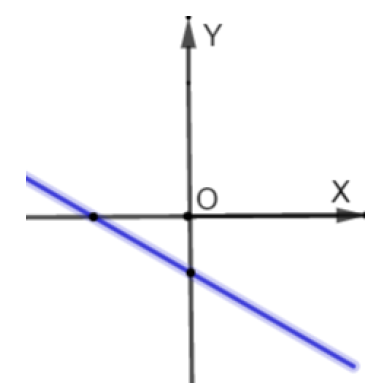
\includegraphics[scale=0.35]{gr7-89.png}}
\end{figure}\\
На рисунке изображен график функции $y=kx+d.$\\
а) Определите знак коэффициента $d.$\\
б) Проходит ли график через точку с координатами $(1; d) ?$\\
90. На координатной прямой выбраны точки $A(x + 1),\ B(x - 3)$ и $C(2x + 3).$ Найдите значения $x,$ при которых $AB = BC.$\\
91. На координатной прямой выбраны точки $A(x + 1),\ B(x - 3)$ и $C(2x + 3).$ Найдите значения $x,$ при которых $AB = AC.$\\
92. Постройте график функции: $y=\cfrac{2x^3+x^2-2x-1}{1-x^2}.$\\
93. Постройте график функции: $y=\cfrac{x^3-x^2-x+1}{1-x^2}.$\\
94. Изобразите на координатной плоскости множество точек, удовлетворяющих уравнению \\$\cfrac{(4+x(2y-x)-y^2)(x^2+y^2-2(x+y-1))}{3x+y+xy+3}=0.$\\
95. Изобразите на координатной плоскости множество точек, удовлетворяющих уравнению \\ $\cfrac{(4-x(2y+x)-y^2)}{(2x-2y+xy-4)(x^2+y^2-2(x+y-1))}=0.$
\newpage
\section{Стандартные задачи}
1. В овощной магазин завезли картофель и морковь. В первый день продали $40\%$ картофеля и $\cfrac{2}{3}$ моркови, что составило 20т. Во второй день продали $\cfrac{2}{3}$ оставшегося картофеля и всю оставшуюся морковь --- всего 15т. Сколько картофеля и сколько моркови было завезено в магазин?\\
2. В город отправляли арбузы и дыни. В первый день отправили $\cfrac{1}{3}$ всех арбузов и $60\%$ всех дынь, что составило 44т. Во второй день отправили 46т, которые составились из $75\%$ оставшихся арбузов и всех оставшихся дынь. Сколько арбузов и сколько дынь было выделено для отправки в город?\\
3. Велосипедист собирался проехать 210 км с постоянной скоростью. Из-за дождя первую половину пути он ехал со скоростью на $40\%$ меньше намеченной. Чтобы наверстать упущенное, вторую половину пути он ехал со скоростью на $40\%$ больше намеченной. В результате он опоздал к намеченному сроку на 2 часа. С какой скоростью он предполагал ехать?\\
4. Участник авторалли рассчитывал проехать расстояние 360 км с постоянной скоростью. Из-за тумана первую половину дистанции он ехал со скоростью на $20\%$ меньше намеченной. На второй половине пути, чтобы наверстать упущенное время, он увеличил скорость на $20\%$ по сравнению с намеченной. В результате он затратил на весь путь на 15 минут больше, чем предполагал. С какой скоростью он предполагал ехать?\\
5. За 3 часа Люба на мотоцикле проезжает то же расстояние,  что Вадик на велосипеде за 5ч. Скорость мотоцикла на 12 км/ч больше скорости велосипедиста. Определить скорость каждого.\\
6. Костя на <<Жигулях>> за 2 часа проезжает на 50 км больше, чем Ира на BMW за 1 час. Скорость BMW в 1,5 раза больше скорости <<Жигулей>>. Определить скорость каждого.\\
7. Расстояние между городами A и B машина прошла за 1ч 15 мин. Обратный путь машина прошла за 1ч 30 мин. Найдите скорость машины, если известно, что на обратном пути скорость машины была на 10 км/ч меньше.\\
8. Теплоход прошёл расстояние между пунктами A и B по течению за 4ч 30 мин, а из B в A против течения он прошёл за 6ч 18мин. Какова скорость теплохода в стоячей воде, если скорость течения 2,4 км/ч?\\
9. Из посёлка в город выехал автобус со скоростью 60 км/ч. Через час после выезда автобуса из посёлка выехал мотоцикл и догнал автобус через 4 часа после выезда автобуса. С какой скоростью ехал мотоциклист?\\
10. Расстояние между посёлками A и B равно 300 км. Из посёлка A в посёлок B выехал автобус, движущийся с постоянной скоростью 60 км/ч. Через час после выезда автобуса из посёлка B в посёлок A с постоянной скоростью выехал мотоциклист, который встретился с автобусом через 1,5 часа. С какой скоростью ехал мотоциклист?\\
11. Два поезда вышли в разное время навстречу друг другу из двух пунктов, расстояние между которыми 1231 км. Скорость первого поезда 50 км/ч, а второго 59 км/ч. Пройдя расстояние 700 км, первый поезд встретился со вторым. На сколько часов один из них вышел раньше другого?\\
12. Два автомобиля вышли в разное время навстречу друг другу из двух пунктов, расстояние между которыми 910 км. Скорость первого автомобиля 80 км/ч, а второго 90 км/ч. Пройдя расстояние 640 км, первый автомобиль встретился со вторым. На сколько часов один из них вышел позже другого?\\
13. Болельщик хочет успеть на стадион к началу матча. Если он пойдёт из дома пешком со скоростью 5 км/ч, то опоздает на 1 ч, а если поедет на велосипеде со скоростью 10 км/ч, то приедет за 30 мин до начала матча. Чему равно расстояние от дома до стадиона?\\
14. Турист, находящийся в спортивном лагере, должен успеть на железнодорожную станцию. Если он поедет на велосипеде со скоростью 15 км/ч, то опоздает на 30 мин, а если на мопеде со скоростью 40 км/ч, то приедет за 2 ч до отхода поезда. Чему равно расстояние от лагеря до станции?\\
15. Скорость катера по течению реки равна 45,2 км/ч, а против --- 36,2 км/ч. Найти скорость течения реки.\\
16. Скорость катера по течению реки равна 40,6 км/ч, а против --- 32,6 км/ч. Найти скорость течения реки.\\
17. Половину пути мотоциклист ехал со скоростью 45 км/ч, а затем задержался на 10 мин, а поэтому, чтобы наверстать потерянное время, он увеличил скорость на 15 км/ч. Каков весь путь мотоциклиста?\\
18. Автобус прошёл $\cfrac{5}{6}$ пути со скоростью 50 км/ч, а затем задержался на 3 мин. Чтобы прибыть в конечный пункт вовремя, оставшуюся часть пути он шёл со скоростью 60 км/ч. Найдите путь, пройденный автобусом.\\
19. Автомобилист преодолел расстояние от города до посёлка за 1 ч 12 мин, двигаясь с постоянной скоростью. Когда он поехал обратно, пошёл дождь, поэтому автомобилист снизил скорость на 20 км/ч и ехал на 24 мин дольше. Найдите расстояние между городом и посёлком.\\
20. Автомобилист в дождливую погоду преодолел расстояние от города до посёлка за 1 ч 48 мин, двигаясь с постоянной скоростью. Когда он поехал обратно, выглянуло солнце, поэтому автомобилист увеличил скорость на 20 км/ч и доехал на 24 мин быстрее. Найдите расстояние между городом и посёлком.\\
21. Через первую трубу бассейн наполняется за 35 минут. За сколько минут наполняет бассейн вторая труба, если вместе они наполняют его за 10 минут?\\
22. Вася съедает торт за 28 минут. За сколько этот торт съедает Петя, если вместе они съедят его за 12 минут?\\
23. Скорость течения реки составляет $5\%$ от скорости катера. Двигаясь против течения, катер за 3 часа проходит на 40 км меньше, чем за 3 часа 40 минут по течению. Найдите скорость катера против течения.\\
24. Скорость течения реки составляет $10\%$ от скорости лодки. Двигаясь против течения реки, лодка за 3 часа 20 минут проходит на 28 км меньше, чем за 4 часа движения по течению. Найдите скорость лодки по течению.\\
25. Маше задано выучить английские глаголы и существительные. Утром она выучила $\cfrac{1}{12}$ всех глаголов и $\cfrac{1}{16}$ всех существительных, всего 5 слов. Вечером она выучила ещё $\cfrac{1}{4}$ всех оставшихся глаголов и $\cfrac{1}{5}$ всех оставшихся существительных. Оказалось, что вечером Маша выучила на 8 глаголов больше, чем существительных. Сколько существительных и сколько глаголов было задано Маше?\\
26. Васе задано решить задачи по алгебре и геометрии. В первый день он решил $\cfrac{1}{15}$ всех задач по алгебре и $\cfrac{1}{25}$ всех задач по геометрии, получилось 5 задач. Во второй день он решил $\cfrac{1}{7}$ остатка задач по алгебре и $\cfrac{1}{6}$ оставшихся задач по геометрии. Оказалось, что во второй день задач по геометрии Вася решил на 2 больше, чем по алгебре. Сколько задач по алгебре и сколько задач по геометрии было задано?\\
27. Два зайца и пять кроликов съедают одну тарелку моркови за восемь секунд, а семь зайцев и четыре кролика съедают такую же тарелку моркови за четыре секунды. Определите, за сколько секунд с этим же количеством моркови справятся заяц и два кролика (все зайцы едят одинаково быстро, все кролики --- тоже).\\
28. Три зайца и два кролика съедают одну тарелку моркови за двенадцать секунд, а пять зайцев и восемь кроликов съедают такую же тарелку моркови за четыре секунды. Определите, за сколько секунд с этим же количеством моркови справятся два зайца и кролик (все зайцы едят одинаково быстро, все кролики --- тоже).\\
29. Если Вася идёт в спортшколу пешком, а возвращается на трамвае, то всего он затрачивает на дорогу 1,5 часа. Если же он в качестве дополнительной тренировки в обе стороны идёт пешком, то на всю дорогу в спортшколу и обратно домой у него уходит 2,5 часа. Какое время Вася затратит на дорогу в спортшколу и обратно домой, если он весь путь проедет на трамвае?\\
30. Двигаясь с определённой скоростью, пешеход пройдёт намеченный путь за 2,5 ч. Но если через 2 часа от начала пути он уменьшит свою скорость на 4 км/ч, то пройдёт весь путь за 3 часа. Найдите длину пути.\\
31. Двадцать семь карандашей и тридцать три ручки стоят 246 рублей. Сколько стоит карандаш, если он на 2 рубля дешевле ручки?\\
32. Пешеход идёт вдоль дороги. Мимо него проезжают попутные автобусы с интервалом 12 минут. С каким интервалом в минутах автобусы проезжают мимо остановки, если скорость автобуса в шесть раз больше скорости пешехода?\\
33. Грузовик проезжает некоторое расстояние за 10 часов. Если бы он проезжал в час на 10 км больше, то ему потребовалось бы на тот же путь 8 часов. Каким было расстояние и скорость движения грузовика?\\
34. Из двух городов A и B, расстояние между которыми равно 600 км, одновременно навстречу друг другу выехали два поезда. Через 2 ч 24 мин расстояние между ними впервые стало равным 240 км. С какой скоростью идут поезда, если скорость первого поезда на 14 км/ч больше скорости второго?\\
35. Пешеход половину пути шёл со скоростью 3 км/ч, а другую половину пути со скоростью 5 км/ч. Найти длину всего пути, пройденного пешеходом, если всего он находился в пути 8 часов.\\
36. Оксана делает некоторую работу за 7 часов, Марина за 6 часов, а Борис Викторович за 3 часа. После того, как Оксана сделала половину всей работы, к ней присоединились Марина и Борис Викторович. За какое время была сделана вся работа и какую её часть сделала Марина?\\
37. Путь от города до посёлка автомобиль проезжает за 2,5 ч. Если он увеличит скорость на 20 км/ч, то за 2 часа он проедет путь на 15 км больший, чем расстояние от города до посёлка. Найдите это расстояние.\\
38. Из A в B выехали два велосипедиста. Первый половину времени, затраченного на весь путь, ехал со скоростью 25 км/ч, а остальное время --- со скоростью 20 км/ч. Второй первую половину пути ехал со скоростью 20 км/ч, а вторую со скоростью 25 км/ч. Кто из них раньше приехал в B?\\
39. Таня и Люба красят забор за 12 часов, Таня и Катя выкрасят этот же забор за 20 часов, а Люба и Катя --- за 15 часов. За работу всем трём девочкам заплатили 1800 рублей. Сколько денег должна получить каждая девочка?\\
40. От станции к посёлку, удалённому на 104 км, отправились одновременно мотоциклист и автомобилист. Скорость автомобиля на 30 км/ч больше скорости мотоцикла. Прибыв в посёлок, автомобиль сразу повернул обратно и встретил мотоциклиста через 1 ч 36 мин после его выезда со станции. На каком расстоянии от станции произошла встреча?\\
41. Бассейн заполняется водой, поступающей из двух труб. Первая труба может наполнить бассейн за 12 часов, а вторая --- за 20ч. После двух часов работы одной первой трубы была включена вторая труба. Сколько времени ушло на заполнение всего бассейна, и какую часть бассейна заполнила первая труба?\\
42. Лена и Наташа живут в одном доме и учатся в одной школе. Лена доходит от дома до школы за 20 минут, а Наташа --- за 30 минут. Через сколько минут Лена догонит Наташу, если Наташа выйдет из дома на 5 минут раньше Лены?\\
43. Надо застелить ковром пол в комнате, ширина которой на 1 м меньше длины. Если купить ковёр, длина и ширина которого на 50 см меньше длины и ширины комнаты, то он будет на 2550 р дешевле, чем ковёр, покрывающий весь пол. Найдите длину и ширину комнаты, если известно, что 1 $\text{м}^2$ ковра стоит 600р.\\
44. Катер за 3 часа по течению и 5 часов против течения проходит 76 км. Найдите скорость течения и собственную скорость катера, если за 6 часов по течению катер проходит столько же, сколько за 9 часов против течения.\\
45. Петя вышел из школы и пошёл по направлению к дому со скоростью 4 км/ч. Одновременно с ним от дома к школе выехал на мопеде его брат Серёжа со скоростью 42 км/ч. Встретив по дороге Петю, Серёжа доехал до школы, мгновенно развернулся и поехал к дому. Таким образом Серёжа ездил между домом и школой до тех пор, пока Петя не пришёл домой. Сколько раз братья встретятся, пока Петя идёт от школы до дома, если расстояние между зданиями 2,8 км?\\
46. Ребёнок Эрвин за полгода обучения в школе научился доезжать до неё за одно и то же время. Каждое утро он тратит на поездку в метро вдвое больше времени, чем на поездку на троллейбусе, при этом 8 минут, что составляет $\cfrac{2}{9}$ от всей поездки в метро, он тратит на ожидание поездов и подъём на эскалаторе. Сколько времени Эрвин добирается до школы, если на весь пеший путь он тратит на 29 минут меньше, чем проводит в метро?\\
47. Ребёнок Эрвин за полгода обучения в школе научился доезжать из неё до дома за одно и то же время. Каждый вечер он тратит на поездку в метро втрое больше времени, чем на поездку на троллейбусе, при этом 9 минут, что составляет $\cfrac{3}{13}$ от всей поездки в метро, он тратит на ожидание поезда и подъём на эскалаторе. Сколько времени Эрвин добирается до дома, если на весь пеший путь он тратит на 31 минуту меньше, чем проводит в метро.\\
48. Бригада из 5 садовников за 3 часа посадила 30 деревьев. Сколько деревьев посадят 4 садовника за 4 часа?\\
49. Стог сена корова съедает за 6 дней, а коза --- за 12 дней. За сколько дней они съедят стог сена вместе?\\
50. Три бригады вспахали два поля общей площадью 96 га. Первое поле было вспахано за 3 дня, причём работали все вместе. Второе поле вспахали за 6 дней вторая и третья бригады. Если бы все три бригады проработали на втором поле 1 день, то оставшаяся часть второго поля первая бригада могла бы вспахать за 8 дней. Сколько гектаров в день может вспахать первая бригада?\\
51. Два поезда выехали одновременно в одном направлении из городов A и B, которые расположены на расстоянии 60 км друг от друга и одновременно прибыли на станцию C. Если бы один из поездов увеличил скорость на 25 км/ч, а другой на 20 км/ч, то они прибыли бы в C также одновременно, но на два часа раньше. Найдите скорости поездов.\\
52. Карлсон съедает банку варенья за 10 минут, Фрекен Бок --- за 12 минут, а Малыш --- за 15 минут. За сколько минут они съедят банку варенья втроём?\\
53. Петя и Вася вскапывают грядку за 10 минут, а один Петя --- за 15 минут. На сколько минут Вася дольше Пети вскапывает грядку, работая один?\\
54. Два пешехода вышли одновременно из своих сёл А и В навстречу друг другу. После встречи первый шёл 50 минут до села В, а второй шёл 18 минут до села А. Сколько минут они шли до встречи?\\
55. Два пешехода вышли одновременно из своих сёл А и В навстречу друг другу. После встречи первый шёл 45 минут до села В, а второй шёл 20 минут до села А. Сколько минут они шли до встречи?\\
56. Мастер и ученик должны были каждый день вместе делать некоторое число деталей. В первый день ученик работал три часа, а мастер --- два, в результате они сделали 0,9 нужного числа деталей. Во второй день наоборот --- мастер работал три часа, а ученик два и они перевыполнили план на $15\%.$ За какое время справился бы с заданием ученик в одиночку?\\
57. Мастер и ученик должны были каждый день вместе делать некоторое число деталей. В первый день ученик работал три часа, а мастер --- два, в результате они сделали $\frac{4}{5}$ нужного числа деталей. Во второй день наоборот --- мастер работал три часа, а ученик два и они перевыполнили план на $5\%.$ За какое время справился бы с заданием ученик в одиночку?\\
58. Первые 60 {\it км} машина ехала со скоростью 40 {\it км/ч,} а следующие 30 {\it км} --- со скоростью 60 {\it км/ч.} Какова средняя скорость $V$ {\it км/ч} на всём пути? В ответе напишите число $V$ без единиц измерения.\\
59. Первые 80 {\it км} поезд шёл со скоростью 60 {\it км/ч,} а следующие 20 {\it км} --- со скоростью $V$ {\it км/ч.} Известно, что средняя скорость на всём пути равна 50 {\it км/ч.} Найдите $V.$ В ответе напишите число $V$ без единиц измерения.\\
60. Первые 80 {\it км} машина ехала со скоростью 60 {\it км/ч,} а следующие 24 {\it км} --- со скоростью 34 {\it км/ч.} Какова средняя скорость $V$ {\it км/ч} на всём пути? В ответе напишите число $V$ без единиц измерения.\\
61. Первые 100 {\it км} поезд шёл со скоростью 80 {\it км/ч,} а следующие 50 {\it км} --- со скоростью $V$ {\it км/ч.} Известно, что средняя скорость на всём пути равна 72 {\it км/ч.} Найдите $V.$ В ответе напишите число $V$ без единиц измерения.\\
62. Имеется сплав золота и серебра. Золото в сплаве составляет $30\%.$ Если бы в сплаве золота было на 2 {\it г} меньше, а серебра --- на 12 {\it г} больше, золото составляло бы $25\%$ от общей массы этого сплава. Найдите массу первоначального сплава. В ответе запишите количество граммов.\\
63. Имеется сплав меди и олова массой 40 {\it кг.} При добавлении 5 {\it кг} меди процентное содержание меди увеличилось на 10 процентных пунктов. Найдите процентное содержание олова в первоначальном сплаве.\\
64. Имеется сплав золота и серебра. Серебро в сплаве составляет $70\%.$ Если бы в сплаве золота было на 10 {\it г} больше, а серебра --- на 4 {\it г} меньше, серебро составляло бы $50\%$ от общей массы этого сплава. Найдите массу первоначального сплава. В ответе запишите количество граммов.\\
65. Имеется сплав меди и олова массой 60 {\it кг.} При добавлении 12 {\it кг} олова процентное содержание меди уменьшилось на 10 процентных пунктов. Найдите процентное содержание меди в первоначальном сплаве.\\
66. Расстояние между двумя пунктами поезд проходит по расписанию за 2,5 {\it ч.} Однако по прошествии 1 часа 40 минут поезд по техническим причинам снизил скорость на 10 {\it км/ч,} в результате чего он опоздал на 10 минут. Найдите первоначальную скорость поезда.\\
67. Расстояние между пунктами $A$ и $B$ составляет 840 {\it км.} Автомобиль выехал из пункта $A$ в направлении к $B$ со скоростью 60 {\it км/ч.} Спустя некоторое время из пункта $B$ в направлении к $A$ выехал автомобиль со скоростью 65 {\it км/ч.} К моменту их встречи один из них проехал на 60 {\it км} больше другого. На сколько часов позже выехал автомобиль из пункта $B$ по сравнению с автомобилем, выехавшим из пункта $A?$\\
68. Расстояние между двумя пунктами поезд проходит по расписанию за 3,5 {\it ч.} Однако по прошествии 1,5 часа поезд по техническим причинам снизил скорость на 5 {\it км/ч,} в результате чего он опоздал на 8 минут. Найдите первоначальную скорость поезда.\\
69. Расстояние между пунктами $A$ и $B$ составляет 680 {\it км.} Автомобиль выехал из пункта $B$ в направлении к $A$ со скоростью 80 {\it км/ч.} Спустя некоторое время из пункта $A$ в направлении к $B$ выехал автомобиль со скоростью 100 {\it км/ч.} К моменту их встречи один из них проехал на 40 {\it км} больше другого. На сколько часов позже выехал автомобиль из пункта $A$ по сравнению с автомобилем, выехавшим из пункта $B?$\\
70. На какое наибольшее число километров может отплыть лодка от пристани против течения реки, если собственная скорость лодки 9 км/ч, скорость течения реки 1 км/ч, чтобы успеть вернуться через 9 часов?\\
71. На какое наибольшее число километров может отплыть лодка от пристани против течения реки, если собственная скорость лодки 8 км/ч, скорость течения реки 2 км/ч, чтобы успеть вернуться через 4 часа?\\
72. Игорь и Паша могут покрасить забор за 4 часа, Паша и Володя могут покрасить этот же забор за 12 часов, а Володя и Игорь --- за 9 часов. За какое время мальчики покрасят забор, работая втроём?\\
73. Лена и Ира могут обработать грядку клубники за 9 часов, Ира и Оля могут обработать эту же грядку за 4 часа, а Оля и Лена --- за 12 часов. За какое время девочки обработают грядку, работая втроём?\\
74. На практику в издательство пришли две студентки. Оказалось, что одна из них набирает текст в два раза медленнее, чем куратор практики, а вторая --- в три раза медленнее, чем куратор. Им выдали перенабрать рукопись. Работая вдвоём, они выполнили работу за 6 часов. За сколько часов выполнил бы эту работу куратор?\\
75. Два мотоциклиста ехали навстречу друг другу. Скорость каждого мотоциклиста 100 км/ч. Параллельно шоссе проходит железная дорога, по которой ехал длинный товарный поезд. Один из мотоциклистов проехал мимо этого поезда в три раза быстрее, чем другой. Какова скорость поезда?\\
76. Петя доехал на своём велосипеде от дома до школы, двигаясь с постоянной скоростью. Если бы он увеличил скорость на 3 м/с, то он доехал бы до школы в три раза быстрее. Во сколько раз быстрее он доехал бы до школы, увеличив скорость на 6 м/c?\\
77. По плану Василий в $16:00$ должен был выйти из дома и отправиться на дачу. К этому времени с дачи за ним должна была приехать машина. Но Василий от нетерпения уже в $15:00$ отправился пешком машине навстречу. Встретив по пути машину, он сел в нее и приехал на дачу на 10 минут раньше запланированного времени. С какой скоростью ехал автомобиль, если Василий шел со скоростью 6 км/ч?\\
78. На овощебазе хранят капусту, морковь и картофель. Картофель при этом занимает в 2 раза больше ящиков, чем морковь, а на капусту приходится в 3 раза больше ящиков, чем на картофель и морковь вместе взятых. Какой процент всех использованных ящиков отведён под хранение капусты?\\
79. На овощебазе хранят капусту, морковь и картофель. Морковь при этом занимает в 3 раза меньше ящиков, чем картошка, а на капусту приходится в 9 раз больше ящиков, чем на картофель и морковь вместе взятых. Какой процент всех использованных ящиков отведён под хранение капусты?\\
80. Автомобиль ехал по дороге сначала со скоростью 90 км/ч. Когда ему осталось проехать на
20 км больше, чем он уже проехал, автомобиль увеличил скорость на $20\%.$ В результате средняя
скорость на всём пути составила 100 км/ч. Каков был путь?\\
81.  Расстояние между городами равно 200 км. Автомобиль сначала ехал по дороге со скоростью
135 км/ч, затем увеличил скорость на $20\%$ и с такой скоростью доехал до конечной цели. Оказалось,
что средняя скорость на всём пути 150 км/ч. На каком расстоянии от старта автомобиль увеличил
скорость?
\newpage
\section{Нестандартные задачи}
1. Делится ли число $\underbrace{11\ldots11}_{\mbox{{\scriptsize 1998 единиц}}}$: а) на 3; б) на 2; в) на 6.\\
2. Делится ли число $\underbrace{22\ldots22}_{\mbox{{\scriptsize 239 двоек}}}$: а) на 3; б) на 2; в) на 6.\\
3. НОД(a,b)=a. Чему равен НОК (a,b)?\\
4. НОК(a,b)=a. Чему равен НОД (a,b)?\\
5. В классе 35 учеников, из которых 20 занимаются в математическом кружке, 11 --- в кружке <<Умелые руки>>, а 10 ребят в эти кружки не ходят. Сколько математиков занимаются в кружке <<Умелые руки>>?\\
6. В классе 37 учеников, из которых 19 занимаются в физическом кружке, 13 --- в биологическом кружке, а 10 ребят в эти кружки не ходят. Сколько физиков занимаются в биологическом кружке?\\
7. Произведение двух последовательных чётных чисел на 120 меньше произведения двух следующих за ними чётных чисел. Найдите эти числа.\\
8. Произведение двух последовательных нечётных чисел на 144 меньше произведения двух следующих за ними нечётных чисел. Найти эти числа.\\
9. Существуют ли такие натуральные $a$ и $b,$ что $(a+b)(3a-b)=6?$\\
10. Существуют ли такие натуральные $a$ и $b,$ что $(a+b)(3a-b)=10?$\\
11. Из трёхзначного числа вычли сумму его цифр. Может ли разность оказаться равной 189?\\
12. Из трёхзначного числа вычли сумму его цифр. Может ли разность оказаться равной 180?\\
13. Сколько клеток пересекает диагональ в клетчатом прямоугольнике размером $239\times566?$\\
14. Сколько клеток пересекает диагональ в клетчатом прямоугольнике размером $239\times366?$\\
15. Какое наибольшее количество точек пересечения могут иметь 9 окружностей?\\
16. Дана последовательность целых чисел: 0; 1; -1; 2; -2; 3; -3... Какое число будет на 366 месте? На каком месте в этой последовательности встретится число 366?\\
17. Дана последовательность целых чисел: 0; 1; -1; 2; -2; 3; -3... Какое число будет на 239 месте? На каком месте в этой последовательности встретится число 239?\\
18. Известно, что числитель дроби $\cfrac{5k^2+7k+11}{8k^2+6k+2}$ делится на 13. Докажите, что дробь можно сократить на 13.\\
19. Известно, что числитель дроби $\cfrac{3k^2+7k+1}{8k^2+4k+10}$ делится на 11. Докажите, что дробь можно сократить на 11.\\
20. Средний возраст одиннадцати игроков <<Зенита>> --- 22 года. Во время матча один из игроков был удалён и ушёл с поля. Средний возраст оставшихся на поле игроков стал равен 21 году. Сколько лет удалённому футболисту?\\
21. Средний  возраст одиннадцати игроков <<Зенита>> --- 26 лет. Во время матча один из игроков был удалён и ушёл с поля. Средний возраст оставшихся на поле игроков стал равен 25 годам. Сколько лет удалённому футболисту?\\
22. Куплено несколько одинаковых книг и одинаковых тетрадей. За книги заплачено 1072 рубля. Сколько куплено книг, если цена одной книги более чем на 100 рублей превосходит цену тетради, а книг куплено на 6 больше, чем тетрадей? Стоимость книг и тетрадей составляет целое число рублей.\\
23. Куплено несколько одинаковых книг и одинаковых тетрадей. За книги заплачен 1071 рубль. Сколько куплено книг, если цена одной книги более чем на 100 рублей превосходит цену тетради, а книг куплено на 5 больше, чем тетрадей? Стоимость книг и тетрадей составляет целое число рублей.\\
24. На складе имеются 33 коробки массой 19 кг каждая и 27 коробок массой 49 кг каждая. Все эти коробки разложили в два штабеля. Обозначим за $S_1$ и $S_2$ суммарные массы коробок в первом и втором штабеле соответственно, и пусть $A=|S_1-S_2|.$\\
а) Найдите наименьшее возможное значение числа $A,$ если в каждом штабеле находится 30 коробок.\\
б) Может ли $A$ равняться нулю, если коробки распределены по штабелям не обязательно поровну?\\
25. На складе имеются 25 коробок массой 13 кг каждая и 19 коробок массой 29 кг каждая. Все эти коробки разложили в два штабеля. Обозначим за $S_1$ и $S_2$ суммарные массы коробок в первом и втором штабеле соответственно, и пусть $A=|S_1-S_2|.$\\
а) Найдите наименьшее возможное значение числа $A,$ если в каждом штабеле находится 22 коробки.\\
б) Может ли $A$ равняться нулю, если коробки распределены по штабелям не обязательно поровну?\\
26. По кругу каким-то образом расставили все натуральные числа от 1 до 15 (каждое число встречается один раз). Для каждой пары соседних чисел нашли разность большего и меньшего. а) Могли ли все полученные разности быть не меньше 7? б) Могли ли все полученные разности быть не меньше 8? Не забудьте объяснить свой ответ.\\
27. По кругу каким-то образом расставили все натуральные числа от 1 до 17 (каждое число встречается один раз). Для каждой пары соседних чисел нашли разность большего и меньшего. а) Могли ли все полученные разности быть не меньше 8? б) Могли ли все полученные разности быть не меньше 9? Не забудьте объяснить свой ответ.\\
28. Назовём трёхзначное натуральное число {\it хорошим,} если оно кратно трём и первые две его цифры отличаются на единицу. Найдите количество хороших чисел, запись которых заканчивается на 7 или на 8.\\
29. Назовём трёхзначное натуральное число {\it интересным,} если оно кратно трём и первые две его цифры отличаются на два. Найдите количество интересных чисел, запись которых заканчивается на 6 или на 7.\\
30. Имеются каменные глыбы: 50 штук по 700 кг каждая, 60 штук по 1000 кг каждая, 80 штук по 1500 кг каждая. Глыбы нельзя раскалывать. Считается, что глыбы можно погрузить в грузовик, если их общая масса не превосходит грузоподъёмности этого грузовика. а) Докажите, что все эти глыбы можно одновременно погрузить на 44 грузовика грузоподъёмностью 5 тонн каждый. б) Докажите, что все эти глыбы нельзя одновременно погрузить на 43 грузовика грузоподъёмностью 5 тонн каждый.\\
31. Имеются каменные глыбы: 50 штук по 800 кг каждая, 60 штук по 1000 кг каждая, 60 штук по 1500 кг каждая. Глыбы нельзя раскалывать. Считается, что глыбы можно погрузить в грузовик, если их общая масса не превосходит грузоподъёмности этого грузовика. а) Докажите, что все эти глыбы можно одновременно погрузить на 39 грузовиков грузоподъёмностью 5 тонн каждый. б) Докажите, что все эти глыбы нельзя одновременно погрузить на 38 грузовиков грузоподъёмностью 5 тонн каждый.\\
32. При умножении двух натуральных чисел, одно из которых на 10 меньше другого, ученик ошибочно уменьшил цифру десятков произведения на 4. Для проверки ответа он поделил полученное неправильное произведение на меньший множитель и получил в частном 39, а в остатке 22. Какие числа он умножал?\\
33. При умножении двух натуральных чисел, одно из которых на 10 больше другого, ученик ошибочно уменьшил цифру десятков произведения на 6. Для проверки ответа он поделил полученное неправильное произведение на меньший множитель и получил в частном 49, а в остатке 22. Какие числа он умножал?\\
34. Шарики можно разложить в пакетики, а пакетики упаковать в коробки, по 2 пакетика в одну коробку. Можно эти же шарики разложить в пакетики так, что в каждом пакетике будет на 3 шарика меньше, чем раньше, но тогда в каждой коробке будет по 3 пакетика, а коробок потребуется на 1 меньше. Какое наибольшее и наименьшее количество шариков может быть при таких условиях?\\
35. Шарики можно разложить в пакетики, а пакетики упаковать в коробки, по 3 пакетика в одну коробку. Можно эти же шарики разложить в пакетики так, что в каждом пакетике будет на 3 шарика больше, чем раньше, но тогда в каждой коробке будет по 2 пакетика, а коробок потребуется на 1 больше. Какое наибольшее и наименьшее количество шариков может быть при таких условиях?\\
36. У Васи есть мишень для игры в <<Дартс>>, в которой есть два центральных сектора (синий и чёрный) и 20 наружных секторов, пронумерованных числами от 1 до 20. За попадание в синий центральный сектор игрок получает 25 очков, за попадание в чёрный центральный сектор --- 50 очков. За попадание в наружный сектор игрок получает количество очков, равное номеру этого сектора, при этом в каждом из наружных секторов есть зоны удвоения и утроения, которые, соответственно, удваивают или утраивают номинал сектора. Например, за попадание в сектор 7 (не в зоны удвоения или утроения) игрок получает 7 очков, за попадание в зону удвоения сектора 7 игрок получает 14 очков, а за попадание в зону утроения сектора 7 --- 21 очко. В центральных секторах зон удвоения и утроения нет. Вася хочет за несколько бросков набрать ровно 881 очко. Какое наименьшее количество бросков ему потребуется для этого?\\
37. У Васи есть мишень для игры в <<Дартс>>, в которой есть два центральных сектора (синий и чёрный) и 20 наружных секторов, пронумерованных числами от 1 до 20. За попадание в синий центральный сектор игрок получает 25 очков, за попадание в чёрный центральный сектор --- 50 очков. За попадание в наружный сектор игрок получает количество очков, равное номеру этого сектора, при этом в каждом из наружных секторов есть зоны удвоения и утроения, которые, соответственно, удваивают или утраивают номинал сектора. Например, за попадание в сектор 7 (не в зоны удвоения или утроения) игрок получает 7 очков, за попадание в зону удвоения сектора 7 игрок получает 14 очков, а за попадание в зону утроения сектора 7 --- 21 очко. В центральных секторах зон удвоения и утроения нет. Вася хочет за несколько бросков набрать ровно 824 очка. Какое наименьшее количество бросков ему потребуется для этого?\\
38. Агата добиралась от дома до института на своём автомобиле с постоянной скоростью 100 км/ч. Обратно она ехала с постоянной скоростью, которая измерялась целым числом километров в час, причём путь до дома занял у неё больше времени, чем путь до института.\\
а) Могла ли её средняя скорость за эти две поездки составить 90 км/ч?\\
б) Могла ли её средняя скорость за эти две поездки оказаться равной целому числу километров в час?\\
39. Настя добиралась от дома до института на своём автомобиле с постоянной скоростью 80 км/ч. Обратно она ехала с постоянной скоростью, которая измерялась целым числом километров в час, причём путь до дома занял у неё больше времени, чем путь до института.\\
а) Могла ли её средняя скорость за эти две поездки составить 70 км/ч?\\
б) Могла ли её средняя скорость за эти две поездки оказаться равной целому числу километров в час?\\
40. В школе была проведена контрольная по математике для всех восьмиклассников. Треть всех участников и ещё 12 учеников получили двойки; четверть участников и ещё 18 учеников получили тройки, а некоторые даже получили четвёрки. Кого оказалось больше: получивших двойку или получивших тройку?\\
41. В школе была проведена контрольная по математике для всех восьмиклассников. Треть всех участников и ещё 20 учеников получили двойки; четверть участников и ещё 30 учеников получили тройки, а некоторые даже получили четвёрки. Кого оказалось больше: получивших двойку или получивших тройку?\\
42. Набор различных натуральных чисел будем называть хорошим, если этот набор можно разбить на две части так, что суммы чисел в каждой из этих частей равны друг другу.\\
а) Приведите пример хорошего набора, в котором нет числа 2.\\
б) Является ли хорошим набор $\{2,\ 3,\ 4,\ 10\}?$\\
в) Приведите пример хорошего набора, который можно разбить на части так, чтобы суммы чисел в этих частях были равны и сами эти части были хорошими.\\
43. На планете Омега некой далёкой галактики жители так же, как и земляне, умеют считать, знают такие же числа, но из известных на Земле операций над числами знают только умножение. А складывать, вычитать и делить они не умеют. Впрочем, у них есть своя операция <<галочка>>, $\vee.$ Про эту операцию известно, что 1) $x\vee x=1$ и 2)
$(x\vee y)\cdot z=x\cdot(z\vee y).$ Вычислите $18\vee 3.$\\
44. На доске написано несколько различных натуральных чисел, произведение любых
двух из которых больше 40 и меньше 100.\\
а) Может ли доске быть 5 чисел?\\
б) Может ли на доске быть 6 чисел?\\
45. Найдите количество натуральных трёхзначных чисел, которые одновременно делятся на 3, на 4 и на 5.\\
46. Сократите дробь $\cfrac{x^{47}+x^{46}+\ldots+x+1}{x^{15}+x^{14}+\ldots+x+1}.$\\
47. Антон  ввёл новую операцию $\#,$ такую, что $x\#y=2x+y.$ Найдите $2\#(3\#4).$\\
48. Назовём натуральное число {\it счастливым,} если его сумма цифр равна 30. Найдите наименьшее счастливое число.\\
49. Найдите наибольшее значение выражения $\cfrac{n+1}{n-4},$ где $n$ --- натуральное число.\\
50. В числе $2^{30}\cdot5^7$ стёрли все нули. Найдите его самую правую цифру.\\
51. Белоснежка хочет связать подарок на Новый год всем семи гномам и принцу. Она умеет вязать одноцветные носки, свитер и жилетку, причём у неё есть нитки трёх цветов --- красного, синего и зелёного.

Белоснежка связала по одному изделию каждого цвета так, что у неё получилось 9 подарков. Один она решила оставить себе, причём ей не важно, то и какого цвета это будет, однако гномам и принцу она хочет угодить. Белоснежка знает, что:\\
1. Принц хотел бы или зелёную жилетку, или синие носки.\\
2. Умник любит только синий, но он не любит свитеры.\\
3. Скромник хотел бы жилетку.\\
4. Простачок хотел бы или жилетку, или свитер синего цвета.\\
5. Чихун и Весельчак хотят одежду одного цвета, причём не любят красный.\\
6. Соня не хотел бы иметь в качестве подарка красные носки.\\
7. Весельчак не хочет свитер.\\
8. Ворчуну невозможно угодить, можно подарить что останется.\\
После того, как она распределила подарки, оказалось, что ей досталась зелёная жилетка. Кто какой подарок получит на Новый год?\\
52. Выписали все числа от 300 до 1100. Сколько раз написали цифру 4?\\
53. Найти сумму $\cfrac{1}{3}+\cfrac{1}{8}+\cfrac{1}{15}+\ldots+\cfrac{1}{n^2-1}$ для каждого натурального $n,$ большего 3.\\
54. Является ли число $3^{4^5}$ точным квадратом?\\
55. Найдите наименьшее натуральное число, большее 2, остатки от деления которого на 3 и на 23 равны 2.\\
56. Сравните $633^{3^{72}}$ и $632^{4^{54}}.$\\
57. При каких натуральных $n$ дробь $\cfrac{4n-23}{n-2}$ является натуральным числом?\\
58. Дан прямоугольник $3 \times 4$ клетки. Можно ли расставить числа $3$ и $-3$ в его клетки так, чтобы все 7 сумм (по строкам и по столбцам) были различны?\\
59. Укажите какое-либо целое число $b$ такое, что число $b^2+3b+2004$ является точным квадратом.\\
60. Расположите 6 точек на 4 отрезках, не лежащих на одной прямой, так, чтобы каждому отрезку принадлежало ровно 3 точки.\\
61. Разрежьте по клеточкам квадрат $6\times 6$ на восемь прямоугольников, среди которых нет одинаковых.\\
62. Найдите сумму утроенного наибольшего общего делителя и половины наименьшего общего кратного чисел 72, 80, 96.\\
63. Найти все трёхзначные числа, делящиеся на 15, сумма первой и третьей цифры у которых равна 7.\\
64. Найти $\left( \cfrac{1\cdot2\cdot4+2\cdot4\cdot8+\ldots+10\cdot20\cdot40}{1\cdot4\cdot5+2\cdot8\cdot10+\ldots+10\cdot40\cdot50}\right)^2.$\\
65. Найти последнюю цифру числа $11^{50}+9^{35}-2^{15}.$\\
66. Сколько существует двузначных чисел, которые при перестановке цифр увеличиваются не менее, чем в три раза?\\
67. Учащимся школы раздали тетради так, что учащиеся одного класса получили равные количества тетрадей, а учащиеся разных классов --- разные. Известно, что 12 девятиклассников и 5 пятиклассников получили вместе 120 тетрадей. Сколько тетрадей получил каждый из этих учащихся?\\
68. Сумма трёх различных целых положительных чисел равна 80. Какое наибольшее значение может принять сумма трёх их попарных разностей? В каждой разности из большего числа вычитается меньшее. Обоснуйте свой ответ.\\
69. Если перемножить цифры некоторого натурального числа на само число, то получится 10472. Найдите все числа, обладающие таким свойством. Ответ обоснуйте.\\
70. В устройстве памяти хранятся данные, занимающие ровно 500 байт. Контроллер, управляющий памятью, позволяет или записать в память сообщение длиной 198 байт, или считать сообщение длиной 300 байт и удалить его. Какой минимальный объём памяти может быть занят в этом устройстве? Можно ли полностью очистить память? Ответ обоснуйте.\\
71. Найдите нечётное простое число $n,$ такое, что $8^7+2^{19}+4^9$ делится на $n.$\\
72. Найти какое-либо натуральное число, которое при делении на каждое из чисел 2, 3, 4, 5, 6 даёт остаток 1, если на 7 это число делится нацело.\\
73. Докажите, что число $1000^{1000}-1$ является составным. Укажите не менее пяти его делителей.\\
74. Докажите, что сумма квадратов трёх последовательных целых чисел при делении на 3 даёт остаток 2.\\
75. Натуральное число $n$ при делении на 7 даёт в остатке 3. Какой остаток при делении на 7 будет давать число $n^2+2n?$\\
76. 90 одинаковых ластиков стоят 156 рублей с копейками. Найдите стоимость одного такого ластика.\\
77. Найдите наименьшее целое, не равное нулю, число $T,$ для которого число $12960\times T$ является квадратом целого числа.\\
78. Найдите все такие двузначные числа, что при перестановке цифр в каждом из них этого число: а) увеличивается на 9; б) уменьшается на 63.\\
79. Число получено перемножением всех чисел $93\cdot94\cdot95\cdot\ldots\cdot162.$ Определите:
а) самый большой простой делитель этого числа;\\
б) наибольшую степень числа 5, на которую делится данное число;\\
в) 15 последних цифр в десятичной записи этого числа.\\
Ответы обоснуйте.\\
80. Найдите последнюю цифру числа $1567^{2008}+2010^{2009}.$\\
81. Таня, Коля, Серёжа и Вика отправились на рыбалку. На рыбалке каждому удалось поймать по одной рыбе, и домой они принесли окуня, щуку, плотву и леща. Серёжа точно не мог поймать щуку, так как он боится их больше всего на свете. Вика поймала одну из хищных рыб (щуку или окуня). Кто кого мог поймать, если Таня поймала окуня?\\
82. Толя, Катя, Семён и Вася отправились на рыбалку. На рыбалке каждому удалось поймать по одной рыбе, и домой они принесли окуня, щуку, плотву и леща. Катя точно не могла поймать плотву, потому что она боится красноглазых рыб (остальные рыбы не красноглазые). Семён поймал одну из хищных рыб (щуку или окуня). Кто кого мог поймать, если Вася поймал леща?\\
83. Вовочка получил единицу. Сколько пятёрок подряд надо ему получить, чтобы его средний балл стал равен 4,5?\\
84. Известно, что среди трёх следующих утверждений есть верное: а) за 4 одинаковых фломастера заплатили 15 р. 86 к. б) за 6 таких же фломастеров заплатили 14 р. 58 к. в) за 8 таких фломастеров заплатили 18 р. 68 к. Какое наибольшее число таких фломастеров можно купить, имея 50 рублей?\\
85. Какие из следующих утверждений верны? Ответ {\bf кратко} обосновать.\\
а) Середина гипотенузы прямоугольного треугольника равноудалена от всех его вершин.\\
б) $8^7-2^{18}$ делится на 7.\\
в) Если сторона и три угла одного треугольника равны стороне и трём углам другого треугольника, то такие треугольники равны.\\
86. Числа от 1 до 37 записаны в строку так, что сумма любых первых нескольких чисел делится на следующее за ними число. Какое число стоит на третьем месте, если на первом месте написано число 37, а на втором --- число 1?\\
87. Каково наименьшее натуральное $n$ такое, что $n!$ делится на 990?\\
88. На доске написаны числа $1, 2, 3,\ldots, 30.$ Вася обводит числа на доске по три штуки так, чтобы суммы всех обведённых групп были различны и не превосходили 35. Какое наибольшее количество групп он может обвести?\\
89. На доске написаны числа $1, 2, 3,\ldots, 40.$ Вася обводит числа на доске по три штуки так, чтобы суммы всех обведённых групп были различны и не превосходили 42. Какое наибольшее количество групп он может обвести?\\
90. Найдите наименьшее общее кратное чисел 12, 70, 135.\\
91. Найдите наибольший общий делитель чисел 2040 и 4200.\\
92. Найдите наименьшее общее кратное чисел 18, 30, 175.\\
93. Найдите наибольший общий делитель чисел 2160 и 10400.\\
94. Найдите все числа вида $\overline{723a1b}\ (a,b$ --- цифры), которые кратны 45.\\
95. Найдите все числа вида $\overline{65a8b}\ (a,b$ --- цифры), которые кратны 36.\\
96. Найдите все числа вида $\overline{6a57b}\ (a,b$ --- цифры), которые кратны 45.\\
97. Найдите все числа вида $\overline{8a56b}\ (a,b$ --- цифры), которые кратны 36.\\
98. При каких натуральных $x$ число $2x-20$ кратно числу $x+5?$\\
99. При каких целых $k$ число $k+11$ кратно числу $k+13?$\\
100. При каких натуральных $x$ число $3x+7$ кратно числу $x-2?$\\
101. При каких целых $k$ число $2k-1$ кратно числу $k+3?$\\
102. Определите, может ли\\
а) число, составленное из одних восьмёрок, делиться на число, составленное из одних троек?\\
б) А наоборот? Ответы не забудьте обосновать.\\
103. Квадраты со сторонами 12 и 15 пересекаются. При удалении из квадратов их общей части получаются две области. Вычислите разность их площадей.\\
104. Про числа $x, y$ и $z$ известно, что выполнены три условия: $\cfrac{x}{y^2+1}=z,\ \cfrac{y}{z^2+1}=x$ и $\cfrac{z}{x^2+1}=y.$ Найдите эти числа.\\
105. Определите, может ли\\
а) число, составленное из одних четвёрок, делиться на число, составленное из одних девяток?\\
б) А наоборот? Ответы не забудьте обосновать.\\
106. Квадраты со сторонами 11 и 14 пересекаются. При удалении из квадратов их общей части получаются две области. Вычислите разность их площадей.\\
107. Про числа $a,\ b$ и $c$ известно, что выполнены три условия: $\cfrac{a}{b^2+1}=c,\ \cfrac{b}{c^2+1}=a$ и $\cfrac{c}{a^2+1}=b.$ Найдите эти числа.\\
108. Докажите, что если $\cfrac{a^2-4b^2}{ab}=3,$ а числа $a$ и $b$ положительные, то $\cfrac{a^2+b^2}{ab}=\cfrac{17}{4}.$\\
109. На доске были написаны несколько различных натуральных чисел. Эти числа разбили на три группы, в каждой из которых оказалось хотя бы одно число.
К каждому числу из первой группы приписали справа цифру 3, к каждому числу из второй группы --- цифру 7, а числа из третьей группы оставили без изменений.\\
а) Могла ли сумма всех этих чисел увеличиться в 8 раз?\\
б) Могла ли сумма всех этих чисел увеличиться в 17 раз?\\
110. Вычислите $\cfrac{x+3y-z}{2x-3z},$ если $\cfrac{x}{2}=\cfrac{y}{3}=\cfrac{z}{4}.$\\
111. Пятеро ребят стоят в ряд и держат воздушные шарики. У ребят, стоящих справа от Пети, 21 шарик, справа от Коли --- 32 шарика, справа от Жени --- 13 шариков, а справа от Севы --- 5 шариков. По сколько шариков держат Сева, Женя и Петя?\\
112. Пять одинаковых маленьких прямоугольников расположены внутри прямоугольника $22\times18$ так, как показано на рисунке. Чему равна площадь одного маленького прямоугольника?\\
\begin{figure}[ht!]
\center{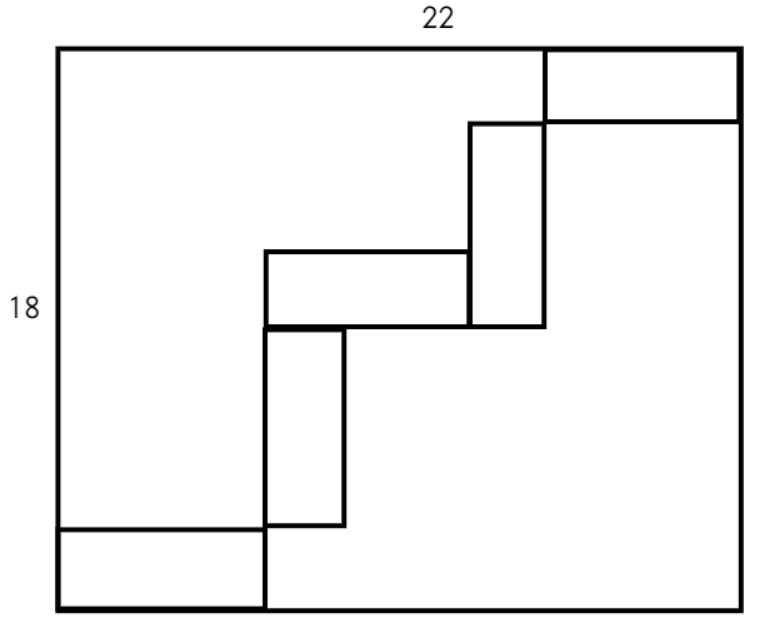
\includegraphics[scale=0.35]{nest7-112.png}}
\end{figure}\\
113. Для натуральных чисел $a,\ b,\ c$ верно равенство $a+\cfrac{1}{b+\cfrac{1}{c}}=\cfrac{35}{11}.$ Чему может быть равно $abc?$\\
114. Найдите все пары натуральных чисел, удовлетворяющих условию $(x-2y)(x-3)=6.$\\
115. Сколько среди чисел 30303032, 246801, 56781234, 67812345 точных квадратов?\\
116. Сумма квадратов цифр трёхзначного числа равна 101. Если из этого числа вычесть 198, то получится трёхзначное число, записанное теми же цифрами, но в обратном порядке. Каким было исходное число?\\
117. Найдите наименьшее натуральное число, большее 6, остатки от деления которого и на 7, и на 17 равны 6. Не забудьте обосновать свой ответ.\\
118. Найдите наименьшее натуральное число, большее 4, остатки от деления которого и на 5, и на 19 равны 4. Не забудьте обосновать свой ответ.\\
119. Вычислите: $\cfrac{1}{6}\cdot 7^{32}-(7+1)(7^2+1)(7^4+1)(7^8+1)(7^{16}+1)=?$\\
120. Вычислите: $\cfrac{1}{4}\cdot 5^{32}-(5+1)(5^2+1)(5^4+1)(5^8+1)(5^{16}+1)=?$\\
121. Известно, что для некоторого натурального $n$ дробь $\cfrac{n - 5}{2n - 1}$ --- целая. Чему она может быть
равна?\\
122. Известно, что для некоторого натурального $n$ дробь $\cfrac{n - 1}{2n - 5}$ --- целая. Чему она может быть
равна?\\
123. Имеется 12 сосисок длиной $X$ см каждая. Их требуется разделить между $X$ котятами, $X$ кошками и $X$ котами так, чтобы каждому котёнку достался кусок сосиски длиной 3 см, каждой кошке ---
кусок сосиски длиной 4 см, а каждому коту --- кусок сосиски длиной 5 см. Можно ли это сделать, если а) $X = 14;$ б) $X = 11?$\\
124. Имеется 10 сосисок длиной $X$ см каждая. Их требуется разделить между $X$ котятами, $X$ кошками и $X$ котами так, чтобы каждому котёнку достался кусок сосиски длиной 2 см, каждой кошке ---
кусок сосиски длиной 3 см, а каждому коту --- кусок сосиски длиной 5 см. Можно ли это сделать, если а) $X = 14;$ б) $X = 11?$
\newpage
\section{Геометрия задачи}
1. Доказать, что если медиана треугольника является высотой, то треугольник равнобедренный.\\
2. Доказать, что если высота треугольника является биссектрисой, то треугольник равнобедренный.\\
3. Точка $D$ лежит на стороне $AB$ треугольника $ABC,$ причём $AD=DB=DC,\ DE\parallel BC.$ Доказать, что $DE\perp AC.$\\
4. На сторонах $AB$ и $BC$ равнобедренного треугольника $ABC\ (AB=AC)$ отмечены точки $D$ и $E$ так, что $AD=DE$ и $DE\parallel AC.$ Доказать, что $AE\perp BC.$\\
5. В четырёхугольнике $PRNL\ (PR\parallel NL)$ на стороне $PR$ взята точка $M,$ а на стороне $NL$ --- точка $K.$ Оказалось, что $MN$ --- биссектриса угла $RMK,$ а $ML$ --- биссектриса угла $PMK.$ Найдите длину $LN,$ если $MK=5.$\\
6. В четырёхугольнике $STGQ\ (ST\parallel GQ)$ на стороне $ST$ взята точка $M,$ а на стороне $GQ$ --- точка $K.$ Оказалось, что $MG$ --- биссектриса угла $TMK,$ а $MQ$ --- биссектриса угла $SMK.$ Найти длину $MK,$ если $GQ=12.$\\
7. Докажите, что сумма длин диагоналей выпуклого четырёхугольника больше, чем половина периметра этого четырёхугольника.\\
8. В треугольнике из двух различных вершин проведены отрезки, соединяющие эти вершины с точками на противоположных сторонах. Доказать, что сумма длин этих отрезков меньше периметра треугольника.\\
9. Доказать, что если треугольники $ABC$ и $A_1B_1C_1$ равны, то $AE=A_1E_1,$ где $E$ и $E_1$ --- середины медиан $BD$ и $B_1D_1$ соответственно.\\
10. Доказать, что если треугольники $MNP$ и $M_1N_1P_1$ равны, то $ME=M_1E_1,$ где $E$ и $E_1$ --- середины высот $PH$ и $P_1H_1$ соответственно.\\
11. В прямоугольном треугольнике $ABC$ на гипотенузе $AB$ выбрана точка $D$ так, что
$\Delta ACD$ равносторонний. Докажите, что $\Delta BCD$ равнобедренный.\\
12. В прямоугольном треугольнике $ABC$ на гипотенузе $AB$ выбрана точка $D$ так, что
$\Delta BCD$ равнобедренный с углом $120^\circ.$ Докажите, что $\Delta ACD$ равносторонний.\\
13. Треугольник $ABC$ --- равнобедренный $(AB=BC),\ \angle B=24^\circ.\ CP$ ---
биссектриса треугольника, $PK\parallel BC$ (точка $K$ лежит на стороне $AC$). Найдите угол $\angle KPC.$\\
14. Треугольник $ABC$ --- равнобедренный $(AB=BC),\ \angle C=72^\circ.\ AP$ ---
биссектриса треугольника, $PK\parallel AB$ (точка $K$ лежит на стороне $AC$). Найдите угол $\angle KPA.$\\
15. Существует ли равнобедренный треугольник, в котором биссектриса одного из углов равна одной из сторон треугольника? (Не забудьте доказать полученный Вами ответ).\\
16. В равнобедренном треугольнике биссектриса одного из углов равна одной из сторон треугольника. Верно ли, что этот треугольник --- прямоугольный? (Не забудьте доказать полученный Вами ответ).\\
17. В равнобедренном треугольнике один из углов равен $120^\circ,$ а высота, проведённая к боковой стороне, равна 17 см. Найдите основание треугольника.\\
18. В равнобедренном треугольнике один из углов равен $120^\circ,$ а основание треугольника равно 10 см. Найдите высоту, проведённую к боковой стороне.\\
19. Можно ли два равнобедренных треугольника с равными боковыми сторонами расположить так, чтобы один лежал внутри другого?\\
20. Можно ли треугольник, две стороны которого равны 566 и 566, поместить в треугольник, две стороны которого равны 239 и 566?\\
21. В прямоугольном треугольнике $ABC$ с гипотенузой $BC$ и углом $B,$ равным $60^\circ,$ проведена высота $AD.$ Найдите $DC,$ если $DB=2\text{см}.$\\
22. В прямоугольном треугольнике $ABC$ с гипотенузой $AC,$ равной 12 см, проведена высота $BD.$ Найдите $CD$ и $DA,$ если угол $\angle A=30^\circ.$\\
23. Сколько существует неравных между собой равнобедренных треугольников со стороной 5см и углом $30^\circ ?$\\
24. Сколько существует неравных между собой равнобедренных треугольников со стороной 5см и углом $60^\circ ?$\\
25. В прямоугольном треугольнике $ABC$ с гипотенузой $AC$ угол $A$ равен $60^\circ,\ BC=6\text{см}.\ AL$ --- биссектриса треугольника $ABC.$ Найдите высоту $LH$ треугольника $ALC.$\\
26. В прямоугольном треугольнике $ABC$ с гипотенузой $AC$ угол $A$ равен $60^\circ.$ Через середину $M$ отрезка $AC$ проведён перпендикуляр к нему, пересекающий прямую $BA$ в точке $T.$ $BC=3\text{см}.$ Найдите$MT.$\\
27. В треугольнике $ABC$ углы $A$ и $B$ равны соответственно $48^\circ$ и $76^\circ.$ Найдите угол между биссектрисой и высотой, проведёнными из вершины $C.$\\
28. В треугольнике $ABC$ углы $A$ и $B$ равны соответственно $64^\circ$ и $24^\circ.$ Найдите угол между биссектрисой и высотой, проведёнными из вершины $A.$\\
29. В треугольнике $ABC$ медиана $AM$ перпендикулярна стороне $AC.$ Найти угол $BAC,$ если $AB=2AC.$\\
30. В треугольнике $ABC$ медиана $AM$ составляет со стороной $AB$ угол $30^\circ.$ Найти угол $BAC,$ если $AB=2AC.$\\
31. В четырёхугольнике $ABCD\ AB=BC.$ Лучи $BA$ и $CD$ пересекаются в точке $E,$ а лучи $AD$ и $BC$ --- в точке $F.$ Известно, что $BE=BF$ и $\angle DEF=25^\circ.$ Найдите $\angle EFD.$\\
32. В четырёхугольнике $KLMN\ NK=LK.$ Лучи $KL$ и $NM$ пересекаются в точке $P,$ а лучи $LM$ и $KN$ --- в точке $Q.$ Известно, что $KP=KQ$ и $\angle MPQ=28^\circ.$ Найдите $\angle PQM.$\\
33. В прямоугольном треугольнике один из углов равен $30^\circ.$ Докажите, что в этом треугольнике отрезок серединного перпендикуляра, проведённого к гипотенузе до пересечения с катетом, втрое меньше большего катета.\\
34. В прямоугольном треугольнике один из углов равен $60^\circ.$ Через середину гипотенузы проведён перпендикуляр до пересечения с катетом. Докажите, что больший катет втрое больше длины построенного перпендикуляра.\\
35. Найдите углы равнобедренного треугольника, если один из его внешних углов равен $130^\circ.$\\
36. Найдите периметр равнобедренного треугольника, если две его стороны равны 6см и 10см.\\
37. В треугольнике $ABC$ угол $A$ равен $40^\circ,$ угол $B$ равен $20^\circ,$ а $AB-BC=4.$  Найдите длину биссектрисы угла $C.$\\
38. В треугольнике $MNP$ угол $M$ равен $40^\circ,$ угол $N$ равен $20^\circ,$ а $MN-NP=8.$  Найдите длину биссектрисы угла $P.$\\
39. В остроугольном треугольнике $ABC$ угол $B$ равен $60^\circ.$ Найдите, в каком отношении биссектриса $BL$ делит высоту $AH.$\\
40. В прямоугольном треугольнике $ABC$ с гипотенузой $AC$ угол $A$ равен $60^\circ,\
BC=6\text{см}.\ AL$ --- биссектриса треугольника $ABC.$ Найдите высоту $LH$ треугольника $ALC.$\\
41. Можно ли какой-либо прямоугольный треугольник разрезать на два треугольника, один из которых равносторонний, а другой равнобедренный?\\
42. Может ли одна из биссектрис треугольника делить другую биссектрису пополам?\\
43. В прямоугольном треугольнике гипотенуза равна 4 см, а острый угол --- $30^\circ.$ Высота, проведённая из вершины прямого угла, делит гипотенузу на два отрезка. Найдите длины этих отрезков.\\
44. В прямоугольном треугольнике гипотенуза равна 6 см, а острый угол --- $30^\circ.$ Высота, проведённая из вершины прямого угла, делит гипотенузу на два отрезка. Найдите длины этих отрезков.\\
45. Два угла равнобедренного треугольника пропорциональны числам 5 и 2. Найдите угол между биссектрисами неравных углов.\\
46. В прямоугольнике $ABCD$ сторона $BC$ в 2 раза больше стороны $AB.$ на продолжении стороны $AD$ за точку $D$ выбрана точка $F.$ Пусть $E$ --- середина стороны $AD,\ \angle DFC=30^\circ.$ Найдите $\angle EBF.$\\
47. В прямоугольнике $ABCD\ AD=2AB.$ На стороне $BC$ отмечена точка $M$ так, что $MA$ --- биссектриса $\angle BMD.$ Найдите $\angle BMA.$\\
48. Внешний угол при вершине $B$ прямоугольного треугольника $ABC$ равен $120^\circ,$ биссектриса угла $\angle ABC$ равна 2 см. Найдите длину стороны $AC,$ если известно, что $\angle C=90^\circ.$\\
49. Внешний угол при вершине $B$ прямоугольного треугольника $ABC$ равен $150^\circ,$ биссектриса острого угла $A$ равна 3 см. Найдите длину стороны $CB.$\\
50. На стороне $CB$ прямоугольного треугольника $ABC$ взята точка $P,$ а на гипотенузе $AB$ взята точка $S.$ При этом $\angle B=35^\circ,\ \angle SCB=20^\circ,\ \angle BAP=10^\circ.$ Докажите, что треугольники $ACP$ и $ACS$ равнобедренные.\\
51. На стороне $AB$ четырёхугольника $ABCD$ взята точка $E.$ При этом $CB\perp BA,$ $DE\perp BA.$ Диагональ $AC$ пересекает отрезок $DE$ в точке $M.$ Известно, что
$\angle BCE=40^\circ,$ $\angle EMA=65^\circ,\ \angle EDA=45^\circ.$ Докажите, что треугольники $CEA$ и $CED$ равнобедренные.\\
52. Какие-то две стороны равнобедренного треугольника отличаются на 8 см, а какие-то две составляют в сумме 20 см. Определите все значения, которые может принимать длина основания такого треугольника.\\
53. Какие-то две стороны равнобедренного треугольника составляют в сумме 16 см, а какие-то две отличаются на 6 см. Определите все значения, которые может принимать длина основания такого треугольника.\\
54. В прямоугольном треугольнике $ABC$ с углом $A,$ равным $30^\circ,$ к гипотенузе $AC$ проведена высота $BH.$ На стороне $BC$ выбрана точка $K$ так, что $KC=HC.$ Лучи $AB$ и $HK$ пересекаются в точке $N.$ Найдите отношение отрезков $AH$ и $KN.$\\
55.  В прямоугольном треугольнике $ABC$ с углом $B,$ равным $30^\circ,$ к гипотенузе $AB$ проведена высота $CH.$ На продолжении стороны $BC$ за точку $C$ выбрана точка $K$ так, что $KC=HC.$ Отрезки $AC$ и $HK$ пересекаются в точке $M.$ Найдите отношение отрезков $BH$ и $KM.$\\
56. Биссектриса внешнего угла $ABD$ треугольника $ABC$ пересекает биссектрису угла $ACB$ в точке $K,\ \angle CKB=19^\circ.$ Найдите $\angle BAC.$\\
57. Биссектриса внешнего угла $ACD$ треугольника $ABC$ пересекает биссектрису угла $ABC$ в точке $M,\ \angle BAC=52^\circ.$ Найдите $\angle BMC.$\\
58. Равные отрезки $AB$ и $CD$ пересекаются в их общей середине $E,\ AD=CE.$ прямая, проходящая через точку $E$ и перпендикулярная к $DE,$ пересекает отрезок $BD$ в точке $M.$ Докажите, что расстояние от точки $M$ до прямой $BC$ в два раза меньше длины отрезка $MD.$\\
59. Равные отрезки $AD$ и $BC$ пересекаются в их общей середине $E,\ AB=DE.$ прямая, проходящая через точку $E$ и перпендикулярная к $BE,$ пересекает луч $CD$ в точке $K.$ Докажите, что расстояние от точки $D$ до прямой $KE$ в четыре раза меньше длины отрезка $KC.$\\
60. Точки $B$ и $O$ расположены по разные стороны от прямой $AC,$ при этом  $OA=OB=OC$ и $\angle AOB = 52^\circ.$ Найдите $\angle ACB.$\\
61. Точки $A$ и $O$ расположены по разные стороны от прямой $BC,$ при этом  $OA=OB=OC$ и $\angle ACB= 17  ^\circ.$ Найдите $\angle AOB.$\\
62. Через вершину $B$ треугольника $ABC$ провели прямую $l,$ параллельную $AC.$ Биссектриса угла $\angle BCA$ пересекает прямую $l$ в точке $D.$ Точка $K$ такова, что $B$ --- середина $DK.$ Докажите, что $\Delta CDK$ --- прямоугольный.\\
63. В треугольнике $ABC$ провели медиану $BD.$ Нашлась такая точка $K,$ что $BK\parallel AC$ и $\angle KBA=\angle ABD.$ Докажите, что $\Delta ABC$ --- прямоугольный.\\
64. На стороне $BC$ треугольника $ABC$ расположены точки $P$ и $K$ так, что $AP=BP$ и $KC=AK.$ При этом оказалось, что величина угла $PAK$ равна $30^\circ.$ Найдите угол $BAC.$\\
65. На стороне $PC$ треугольника $PKC$ расположены точки $A$ и $B$ так, что $AP=AK$ и $KB=BC.$ При этом оказалось, что величина угла $AKB$ равна $40^\circ.$ Найдите угол $PKC.$\\
66. В треугольнике $ABC$ угол $B$ равен $30^\circ,$ угол $A$ равен $120^\circ.$ Из вершины $B$ проведена высота $BH,$ при этом оказалось, что $HC=$1дм 2 см. Найдите расстояние от точки $A$ до прямой $BC.$\\
67. Из вершины $K$ треугольника $PTK$ проведена высота $KH,$ при этом оказалось, что $HP=$2дм 1см. Найдите расстояние от точки $T$ до прямой $PK,$ если известно, что угол $K$ равен $30^\circ,$ угол $T$ равен $120^\circ.$\\
68. Из отрезков длиной 3, 5, 6, 11 составили четырёхугольник, одна из диагоналей которого имеет целую длину. Чему может быть равна эта длина?\\
69. Точка $K$ лежит на отрезке $AB,$ а точка $M$ --- на отрезке $BC.$ Отрезки $AM$ и $CK$ пересекаются в точке $P.$ Оказалось, что $\angle ABC=37^\circ,\ \angle BAM : \angle CAM=4:7,$ $\angle ACK: \angle BCK=7:4.$ Найдите величину угла $APC.$\\
70. Точка $M$ лежит на отрезке $AC,$ а точка $P$ --- на отрезке $BC.$ Отрезки $AP$ и $BM$ пересекаются в точке $K.$ Оказалось, что $\angle ACB=26^\circ,\ \angle CAP : \angle BAP=5:6,$ $\angle ABM: \angle CBM=6:5.$ Найдите величину угла $AKB.$\\
71. Точка $M$ --- середина стороны $AC$ треугольника $ABC,$ в котором $\angle B=90^\circ,\ \angle A=30^{\circ}.$ На стороне $AB$ отмечена такая точка $D,$ что $AD=BC.$ Пусть $DP$ --- высота треугольника $MBD.$ Докажите, что удвоенный периметр треугольника $MDP$ больше периметра треугольника $MDB.$\\
72. Точка $D$ --- середина стороны $AB$ треугольника $ABC,$ в котором $\angle C=90^{\circ},\ \angle A=60^{\circ}.$ На стороне $BC$ отмечена такая точка $M,$ что $BM=AC.$ Пусть $MK$ --- высота треугольника $MCD.$ Докажите, что удвоенный периметр треугольника $MDK$ больше периметра треугольника $MDC.$\\
73. На стороне $AB$ квадрата $ABCD$ построен равносторонний треугольник $MAB,$ причём точка $M$ лежит вне квадрата. Найдите углы треугольника $DMC.$\\
74. На стороне $AB$ квадрата $ABCD$ построен равносторонний треугольник $NAB,$ причём точка $N$ лежит внутри квадрата. Найдите углы треугольника $DNC.$\\
75. Острый угол прямоугольного треугольника равен $30^\circ,$ гипотенуза равна 8. Найдите отрезки, на которые делит гипотенузу высота, проведённая из вершины прямого угла.\\
76. Острый угол прямоугольного треугольника равен $60^\circ.$ Высота к гипотенузе делит её на два отрезка, длина большего из которых равна 12. Найдите длину гипотенузы.\\
77. Четырёхугольник $ABCD$ называется дельтоидом, если в нём $BA=AD$ и $BC=CD.$ Докажите, что его диагонали $AC$ и $BD$ перпендикулярны.\\
78. В треугольнике $ABC$ угол $B$ равен $90^\circ,\ CC_1$ --- биссектриса, $CC_1=16$см, $BC_1=8$см. Найдите внешний угол при вершине $A.$\\
79. В треугольнике $ABC\ \angle C=90^\circ,$ проведена высота $CD,\ BC=2BD.$ Найдите $AD,$ если $BC=4.$\\
80. В треугольнике $KLM$ известно, что $KM<ML<LK.$ Укажите наибольший угол треугольника.\\
81. Найдите градусные меры трёх углов треугольника, если два его внешних угла равны соответственно $80^\circ$ и $115^\circ.$\\
82. На сколько частей делят плоскость четыре прямые, являющиеся продолжениями сторон четырёхугольника, никакие две стороны которого не параллельны?\\
83. Две стороны треугольника равны 2 см и 6 см. Третья сторона выражается целым числом сантиметров. Какой может быть её длина? Выпишите все возможные варианты.\\
84. В прямоугольном треугольнике $KLM$ с углами $\angle M=90^\circ$ и $\angle K=60^\circ$ проведена высота $MH,$ причём $KH=6.$ Найдите длину $LH.$\\
85. В треугольнике $ABC$ угол $B$ --- прямой, $BD$ --- высота,  $BC$ в два раза больше $DC.$ Найти отношение длин отрезков $DC$ и $AD.$\\
86. Построить треугольник по двум сторонам и медиане, проведённой к меньшей из них.\\
87. В треугольнике $ABC\ AB=BC,\ \angle C=72^\circ,\ AP$ --- биссектриса, $PK\parallel AB,\ PK$ пересекает сторону $AC$ в точке $K.$ Найдите $\angle KPA.$\\
88. В треугольнике $ABC$ биссектрисы $AA_1$ и $BB_1$ пересекаются в точке $M,$ при этом $\angle AMB=120^\circ.$ Найдите $\angle C.$\\
89. В треугольнике $ABC\ AB=BC,\ AC=8,$ точка $E$ лежит на стороне $BC,$ причём $BE=EC.$ Точка $E$ делит периметр треугольника $ABC$ (считая от вершины $A$) на две части, из которых одна больше другой на 2. Найдите $AB.$\\
90. Как с помощью циркуля и линейки разделить угол в $54^\circ$ на три равные части?\\
91. В треугольнике $ABC$ угол $A$ равен $70^\circ.$ Биссектрисы углов $A$ и $C$ пересекаются в точке $O.$ Угол $AOC$ равен $115^\circ.$ Найдите углы $B$ и $C$ треугольника $ABC,$ а также углы $AOB$ и $BOC.$\\
92. Биссектрисы внешних углов при вершинах $A$ и $B$ равнобедренного треугольника $ABC\ (AB=BC)$ пересекаются в точке $O,$ угол $AOB=70^\circ.$ Найдите углы треугольника $ABC.$\\
93. Длина отрезка $BC$ равна 8. Точка $A$ лежит на прямой $BC,$ но не принадлежит отрезку $BC,$ причём $5AB=AC.$ Точка $D$ принадлежит отрезку $BC$ и $4DC=BC.$ Найдите длину отрезка $AD.$\\
94. На сторонах угла $A,$ равного $127^\circ,$ отмечены точки $B$ и $C,$ а внутри угла --- точка $D$ так, что $\angle ABD=25^\circ,\ \angle ACD=19^\circ.$ На луче $BD$ отмечена точка $P$ так, что точка $D$ лежит между точками $B$ и $P.$ Найдите угол $PDC.$\\
95. В треугольнике $ABC$ высоты $AH$ и $BP$ равны между собой, угол $ABP$ равен углу $CAH.$ Найдите углы треугольника.\\
96. В треугольнике $ABC\ \angle A: \angle B: \angle C=3:5:2.$ На прямой, содержащей медиану $CM,$ отложен отрезок $MK,$ равный $CM.$ Найдите $\angle ABK.$\\
97. В равнобедренном треугольнике $ABC$ с основанием $AB$ проведены биссектрисы $AA_1$ и $BB_1,$ которые пересекаются в точке $O.$ Найти углы треугольника $AOB_1,$ если один из углов треугольника $ABC$ на $30^\circ$ больше другого. Рассмотреть не менее двух случаев.\\
98. В равнобедренном треугольнике биссектриса угла при основании делит медиану, проведённую из другого угла при основании, пополам. Найдите стороны треугольника, если его периметр равен 20 см.\\
99. В треугольнике $ABC\ \angle A: \angle B=2:5,\ \angle B: \angle C=5:11.$ Найдите угол между высотой и биссектрисой, проведёнными из вершины меньшего угла.\\
100. В треугольнике $ABC$ угол $B$ равен $100^\circ.$ На луче $CA$ отмечена точка $M$ так, что $MA=AB,$ и точка $A$ находится между точками $M$ и $C.$ На луче $AC$ отмечена точка $N$ так, что $CN=BC,$ и точка $C$ находится между точками $A$ и $N.$ Найдите градусную меру угла $MBN.$\\
101. В треугольнике $ABC\ AB=BC,$ точка $T$ --- середина стороны $AB,$ точка $H$ --- середина стороны $BC,$ отрезок $TP$ перпендикулярен к стороне $AB,$ отрезок $KH$ перпендикулярен к стороне $BC$ (точки $P$ и $K$ лежат на стороне $AC),\ \angle ABC=120^\circ,\ AC=21$ см. Найдите длину отрезка $PK.$\\
102. Через вершины $A$ и $C$ треугольника $ABC$ проведены прямые, перпендикулярные биссектрисе угла $ABC$ и пересекающие прямые $CB$ и $BA$ в точках $K$ и $M$ соответственно. Найдите $AB,$ если $BM=8,\ KC=1.$\\
103. Дан треугольник $ABC$ с углами $30^\circ,\ 70^\circ$ и $80^\circ$ соответственно. Внутри треугольника взята точка $O,$ такая, что треугольники $AOB,\ AOC$ и $BOC$ являются равнобедренными с общей вершиной $O.$ Найдите углы этих равнобедренных треугольников.\\
104. Треугольник $PQR$ --- прямоугольный $(\angle R=90^\circ),\ \angle PQR=60^\circ,\ QR=6,5.$ Через точку $Q$ проведена прямая, параллельная прямой $PR$ и на ней взята точка $S$ так, что $PR=QS.$\\
а) Между какими целыми числами лежит длина отрезка $QS?$\\
б) Найдите углы треугольника $ROS,$ если $RO$ --- биссектриса треугольника $QRS.$\\
105. Треугольник $KLM$ --- прямоугольный $(\angle M=90^\circ),\ \angle KLM=60^\circ,\ LM=8,5.$ Через точку $L$ проведена прямая, параллельная прямой $KM$ и на ней взята точка $N$ так, что $KM=LN.$\\
а) Между какими целыми числами лежит длина отрезка $LN?$\\
б) Найдите углы треугольника $MON,$ если $MO$ --- биссектриса треугольника $LMN.$\\
106. $BM$ --- медиана в треугольнике $ABC,\ MD$ --- биссектриса угла $AMB,\ ME$ --- биссектриса угла $BMC.$ Найдите угол $DME.$\\
107. Биссектриса угла при вершине треугольника пересекает основание под углом $73^\circ,$ а биссектрису одного из углов при основании под углом $58^\circ.$ Найдите углы треугольника.\\
108. Биссектриса угла при вершине треугольника пересекает основание под углом $71^\circ,$ а биссектрису одного из углов при основании под углом $57^\circ.$ Найдите углы треугольника.\\
109. В $\Delta KHM\ KH=12,\ HM=9,\ MK=18.$ Через точку $A,$ лежащую на стороне $HM,$ проведён перпендикуляр к биссектрисе $\angle M,$ пересекающий сторону $KM$ в точке $C,$ и перпендикуляр к биссектрисе $\angle H,$ пересекающий сторону $KH$ в точке $B.$ В каком отношении точка $A$ делит сторону $HM,$ если $KC=2KB?$\\
110. В $\Delta KHM\ KH=12,\ HM=7,\ MK=17.$ Через точку $A,$ лежащую на стороне $HK,$ проведён перпендикуляр к биссектрисе $\angle K,$ пересекающий сторону $KM$ в точке $B,$ и перпендикуляр к биссектрисе $\angle H,$ пересекающий сторону $MH$ в точке $C.$ В каком отношении точка $A$ делит сторону $HK,$ если $MC=0,5MB?$\\
111. Четырёхугольник $ABCD$ называется дельтоидом, если в нём $AB=BC$ и $AD=DC.$ Докажите, что точка $O$ пересечения диагоналей дельтоида является серединой одной из его диагоналей. \\
112. Точки $A,\ B$ и $C$ лежат на одной прямой, причём точка $C$ расположена вдвое дальше от одной из точек $A$ и $B,$ чем от другой. Найдите $AB,$ если $AC=18.$\\
113. В треугольнике $ABC\ \angle A=40^\circ, \angle C=90^\circ.$ Определите угол между высотой и медианой, проведёнными из вершины угла $C.$\\
114. Постройте с помощью циркуля и линейки треугольник $ABC$ по его стороне $a,$ сумме сторон $b+c$ и высоте, проведённой к стороне $c.$\\
115. В $\Delta SPM:$ мера угла $P$ равна $90^\circ,$ мера угла $M$ равна $60^\circ,$ $ST$ --- биссектриса $\Delta SPM,\ |PT|=26,\ TF$ --- высота $\Delta TSM.$ Найдите $|TF|.$\\
116. В $\Delta MNK:\ |MN|=|NK|=|MK|,\ |MN|=13,\ P$ --- середина $|MK|,\ R\in[NK],\ (PR)\perp(NK).$ Найдите $|KR|.$\\
117. В треугольнике $ABC$ проведена биссектриса $AD,$ а в треугольнике $ADC$ --- биссектриса $DE.$ Оказалось, что $\angle ABD=43^\circ,$ а $DE=CD.$ Найдите $\angle BAC.$\\
118. В треугольнике $ABC$ проведена биссектриса $BE,$ а в треугольнике $BAE$ --- биссектриса $ED.$ Оказалось, что $\angle ECB=22^\circ,$ а $ED=AE.$ Найдите $\angle ABC.$\\
119. Точка $M$ --- середина стороны $AC$ треугольника $ABC.$ Точка $D$ на стороне $BC$ такова, что $\angle BMA=\angle DMC.$ Оказалось, что $CD+DM=BM.$ Докажите, что $\angle ACB+\angle ABM=\angle BAC.$\\
120. В выпуклом пятиугольнике $ABCDE$ известно, что $AE=AD,\ AC=AB$ и $\angle DAC=\angle AEB+\angle ABE.$ Докажите, что сторона $DC$ в два раза больше медианы $AK$ треугольника $ABE.$\\
121. Возможно ли, чтобы медианы острых углов прямоугольного треугольника были перпендикулярны? Приведите пример такого треугольника или докажите, что его не существует.\\
122. Периметр равнобедренного треугольника равен 4{\it дм.} Известно, что разность между длинами двух сторон равна 1{\it дм.} Найдите длины сторон этого треугольника. (В ответе следует указать длины трёх сторон с единицами длины).\\
123. Найдите периметр равнобедренного треугольника, в котором длины двух сторон равны 8{\it см} и 12{\it см.}\\
124. Периметр равнобедренного треугольника равен 25{\it см.} Известно, что разность между длинами двух сторон равна 5{\it см.} Найдите длины сторон этого треугольника. (В ответе следует указать длины трёх сторон с единицами длины).\\
125. Найдите периметр равнобедренного треугольника, в котором длины двух сторон равны 6{\it см} и 14{\it см.}\\
126. Точки $A,\ B,\ C$ расположены на одной прямой. Известно, что $AB=10$ и $AC=4.$ Найдите все возможные значения $BC.$\\
127. В треугольнике $ABC$ проведена биссектриса $BK.$ Известно, что $BK=KC,\ \angle AKB=80^\circ.$ Найдите $\angle BAC.$\\
128. Точки $C,\ D,\ K$ расположены на одной прямой. Известно, что $CD=8$ и $CK=3\cdot DK.$ Найдите все возможные значения $DK.$\\
129. В остроугольном треугольнике $KLM$ проведены высота $KA$ и биссектриса $LB.$ Известно, что они пересекаются в точке $H$ и $\angle AHB=100^\circ.$ Найдите $\angle KLM.$\\
130. В треугольнике $ABC\ \angle B=30^\circ,\ \angle C=60^\circ.$ Через середину стороны $BC$ проведена прямая $p,$ перпендикулярная $BC.$ Прямая $p$ пересекает сторону $AB$ в точке $L.$ Известно, что один из отрезков $BL$ и $AL$ больше другого на 4 {\it см.} Найдите длину отрезка прямой $p,$ находящегося внутри данного треугольника.\\
131. В равнобедренном треугольнике $ABC\ \angle A=30^\circ,\ \angle B=120^\circ,\ BC=8${\it см.} Проведены высота $AK$ данного треугольника и высота $KL$ треугольника $AKB.$ Найдите длину $BL.$\\
132. В треугольнике $KLM\ \angle L=30^\circ,\ \angle K=60^\circ.$ Через середину стороны $KL$ проведена прямая $p,$ перпендикулярная $KL.$ Прямая $p$ пересекает сторону $LM$ в точке $A$ и продолжение стороны $KM$ в точке $B.$ Известно, что $AB=3${\it см.} Найдите длину $AL.$\\
133. В равнобедренном треугольнике $KLM\ \angle K=30^\circ,\ \angle L=120^\circ,\ KL=6${\it см.} Проведены высота $MA$ данного треугольника и высота $AB$ треугольника $LAM.$ Найдите длину $BM.$\\
134. В равнобедренном треугольнике $ABC$ с вершиной $B$ на стороне $BC$ взята точка $K$ такая, что $CA=AK=KB.$ Периметр треугольника $CAK$ равен 4, периметр треугольника $AKB$ равен 5. Вычислите периметр данного треугольника.\\
135. В равнобедренном треугольнике $ABC$ с вершиной $A$ на стороне $AC$ взята точка $K$ такая, что $CB=BK=KA.$ Периметр треугольника $CBK$ равен 6, периметр треугольника $AKB$ равен 7. Вычислите периметр данного треугольника.\\
136. Верно ли, что треугольники $ABC$ и $MKP$ равны, если $AB=3,\ BC=4,\ \angle C=30^\circ;\ MK=3,\ KP=4,\ \angle P=30^\circ?$ Ответ обоснуйте.\\
137. Верно ли, что треугольники $ABC$ и $MKP$ равны, если $AB=5,\ BC=8,\ \angle C=30^\circ;\ MK=5,\ KP=8,\ \angle P=30^\circ?$ Ответ обоснуйте.\\
138. В равнобедренном треугольнике один из углов в два раза меньше другого. Найдите величину наименьшего угла этого треугольника.\\
139. Медиана $AM$ треугольника $ABC$ перпендикулярна его биссектрисе $BK.$ Найдите $AB,$ если $BC=12.$\\
140. В равнобедренном треугольнике один из углов в два раза больше другого. Найдите величину наименьшего угла этого треугольника.\\
141. Биссектриса $AP$ треугольника $ABC$ перпендикулярна его медиане $CK.$ Найдите $AB,$ если $AC=8.$\\
142. Длины сторон треугольника --- последовательные натуральные числа. Найдите периметр треугольника, если известно, что одна из его медиан перпендикулярна одной из его биссектрис.\\
143. Постройте с помощью циркуля и линейки треугольник по двум его углам и периметру.\\
144. Медиана разбивает треугольник на два треугольника. Докажите, что высоты в этих треугольниках, проведённые к этой медиане, равны.\\
145. Биссектриса $BE$ угла $B$ треугольника $ABC$ равна биссектрисе $BF$ его внешнего угла при той же вершине. Найдите разность двух других углов треугольника $ABC.$\\
146. Две стороны четырёхугольника равны 1 и 7. Одна из диагоналей, длина которой равна 3, делит его на два равнобедренных треугольника. Найдите все возможные значения периметра этого четырёхугольника.\\
147. В прямоугольном треугольнике на гипотенузе $AB$ взята точка $K$ такая, что $AK=CK=6.$ Найдите $BK.$\\
148. Биссектриса внешнего угла треугольника параллельна его стороне. К этой же стороне в треугольнике проведена медиана. Найдите угол между этими биссектрисой и медианой.\\
149. В треугольнике две высоты не меньше сторон, на которые они опущены. Найдите углы треугольника.\\
150. В равнобедренном треугольнике $ABC\ \angle B = 100^\circ.$ Определите угол между прямой, содержащей высоту $AA_1,$ и прямой, содержащей биссектрису $BB_1.$\\
151. В равнобедренном треугольнике $ABC\ \angle B = 130^\circ.$ Определите угол между прямой, содержащей высоту $AA_1,$ и прямой, содержащей биссектрису $BB_1.$\\
152. В треугольнике $ABC\ \angle B = 84^\circ,\ BH$ --- высота. Найдите $\angle BAC,$ если $AH=BC+CH.$\\
153. В треугольнике $ABC\ \angle B = 81^\circ,\ BH$ --- высота. Найдите $\angle BAC,$ если $AH=BC+CH.$\\
154. Известно, что в треугольнике один угол на $18^\circ$ больше другого, а также есть два угла, в сумме дающие $144^\circ.$ Какие могут быть углы у треугольника?\\
155. Известно, что в треугольнике один угол на $24^\circ$ больше другого, а также есть два угла, в сумме дающие $132^\circ.$ Какие могут быть углы у треугольника?\\
156. В прямоугольнике $ABCD$ на стороне $BC$ нашлась такая точка $X,$ что $\angle XD = 90^\circ$ и $\angle XAD =2\angle CXD.$ Найдите $BX : XC.$\\
157. В прямоугольнике $ABCD$ на стороне $BC$ нашлась такая точка $X,$ что $\angle XAD = \angle XDC = 60^\circ.$ Известно, что $XC = 30.$ Найдите $XM,$ где $M$ — середина $AD.$\\
158. Точка $M$ --- середина стороны $BC$ треугольника $ABC.$ На отрезке $AC$ нашлась такая точка $D,$ что $DM$ и $BC$ перпендикулярны. Отрезки $AM$ и $BD$ пересекаются в точке $X.$ Оказалось, что
$AC = 2BX.$ Докажите, что $X$ --- середина отрезка $AM.$\\
159. Дан равнобедренный треугольник $ABC.$ На продолжении боковой стороны $BC$ за вершину $B$ выбрана точка $D,\ M$ --- середина основания $AC.$
Отрезок $DM$ пересекает сторону $AB$ в точке $X.$ Оказалось, что $X$ --- середина $DM.$ Докажите, что $2AX = CD.$
\newpage
\section{Числовые выражения решения}
1. $\left(\cfrac{2}{3}-1,3+\cfrac{3}{4}\right):1,4+\cfrac{1}{6}=\left(\cfrac{17}{12}-\cfrac{13}{10}\right):\cfrac{14}{10}+\cfrac{1}{6}=\cfrac{7}{60}\cdot\cfrac{10}{14}+\cfrac{1}{6}=
\cfrac{1}{12}+\cfrac{1}{6}=\cfrac{1}{4}.$\\
2. $4,4-0,28:\left(\cfrac{1}{9}-\cfrac{7}{15}+0,375\right)=4,4-0,28:\left(-\cfrac{16}{45}+\cfrac{3}{8}\right)=4,4-\cfrac{28}{100}:\cfrac{7}{360}=4,4-\cfrac{7}{25}\cdot\cfrac{360}{7}=
\\=4,4-14,4=-10.$\\
3. $\left(1\cfrac{11}{24}+\cfrac{13}{36}\right)\cdot1,44-\cfrac{8}{15}\cdot0,5625=\cfrac{131}{72}\cdot\cfrac{144}{100}-\cfrac{8}{15}\cdot\cfrac{5625}{10000}=
2,62-0,3=2,32.$\\
4. $\left(\cfrac{31}{66}+1\cfrac{10}{33}\right)\cdot1,32-\cfrac{8}{13}\cdot0,1625=\cfrac{117}{66}\cdot\cfrac{132}{100}-\cfrac{8}{13}\cdot\cfrac{1625}{10000}=
2,34-0,1=2,24.$\\
5. $\cfrac{15\cfrac{13}{29}\cdot3,625+28:\cfrac{7}{15}}{\cfrac{20}{49}\cdot9,8+0,625:0,75}=\cfrac{\cfrac{448}{29}\cdot\cfrac{3625}{1000}+28\cdot\cfrac{15}{7}}{\cfrac{20}{49}\cdot\cfrac{98}{10}+\cfrac{625}{1000}:\cfrac{75}{100}}=
\cfrac{56+60}{4+\cfrac{5}{6}}=\cfrac{116}{\cfrac{29}{6}}=24.$ Значит, искомое число равно \\$24:0,048=500.$\\
6. $\cfrac{12\cdot(3,4-1,275)\cdot\cfrac{16}{17}}{\cfrac{5}{18}\cdot\left(1\cfrac{7}{85}
+6\cfrac{2}{17}\right):\cfrac{1}{2}}=\cfrac{12\cdot2,125\cdot\cfrac{16}{17}}{\cfrac{5}{18}\cdot\cfrac{612}{85}\cdot\cfrac{2}{1}}=
\cfrac{12\cdot2,125\cdot\cfrac{16}{17}}{\cfrac{5}{18}\cdot\cfrac{612}{85}\cdot\cfrac{2}{1}}=\cfrac{24}{4}=6.$ Значит, искомое число равно $6:0,024=250.$\\
7. $\left(-5,17:1\cfrac{3}{4}+1,67\cdot\cfrac{4}{7}\right)\cdot\left(-1\cfrac{1}{11}\right)=\left(-5,17\cdot\cfrac{4}{7}+1,67\cdot\cfrac{4}{7}\right)\cdot\left(-1\cfrac{1}{11}\right)=$\\
$=\cfrac{4}{7}\cdot\left(-5,17+1,67\right)\cdot\left(-\cfrac{12}{11}\right)=\cfrac{4}{7}\cdot\left(-\cfrac{7}{2}\right)\cdot\left(-\cfrac{12}{11}\right)=\cfrac{24}{11}.$\\
8. $\left(7,42\cdot\cfrac{5}{9}-(-11,48):1\cfrac{4}{5}\right):0,35=\left(7,42\cdot\cfrac{5}{9}+11,48\cdot\cfrac{5}{9}\right):\cfrac{35}{100}=
\cfrac{5}{9}\cdot\left(7,42+11,48\right)\cdot\cfrac{100}{35}=\cfrac{5}{9}\cdot\cfrac{189}{10}\cdot$\\$\cdot\cfrac{20}{7}=30.$\\
9. $\left(3,14\cdot\cfrac{15}{4}-2,72:\left(-6\cfrac{2}{5}\right)\right):\left(23,9-\cfrac{351}{30}\right)=
\left(\cfrac{314}{100}\cdot\cfrac{15}{4}-\cfrac{272}{100}\cdot\left(-\cfrac{5}{32}\right)\right):\left(\cfrac{239}{10}-\cfrac{117}{10}\right)=$\\
$=\left(\cfrac{471}{40}+\cfrac{17}{40}\right):\cfrac{122}{10}=\cfrac{488}{40}\cdot\cfrac{10}{122}=1.$\\
10. $\left(27,2:5\cfrac{3}{5}-0,314\cdot\left(-\cfrac{50}{7}\right)\right):\left(\cfrac{942}{200}+2,39\right)=
\left(\cfrac{272}{10}\cdot\cfrac{5}{28}-\cfrac{314}{1000}\cdot\left(-\cfrac{50}{7}\right)\right):\left(\cfrac{942}{200}+\cfrac{239}{100}\right)=$\\
$=\left(\cfrac{34}{7}+\cfrac{157}{70}\right):\cfrac{710}{100}=\cfrac{497}{70}\cdot\cfrac{100}{710}=1.$\\
11. $\left(1\cfrac{3}{4}:1,125-1,75:\cfrac{2}{3}\right)\cdot1\cfrac{5}{7}=
\left(\cfrac{7}{4}:\cfrac{1125}{1000}-\cfrac{175}{100}:\cfrac{2}{3}\right)\cdot\cfrac{12}{7}=
\left(\cfrac{7}{4}\cdot\cfrac{8}{9}-\cfrac{7}{4}\cdot\cfrac{3}{2}\right)\cdot\cfrac{12}{7}=
\left(\cfrac{14}{9}-\cfrac{21}{8}\right)\cdot\cfrac{12}{7}=$\\$=-\cfrac{77}{72}\cdot\cfrac{12}{7}=-\cfrac{11}{6}.$\\
12. $19\cfrac{1}{3}:4,75-\left(5\cfrac{1}{3}-3,5\cdot\left(-\cfrac{4}{19}\right)\right)=
\cfrac{58}{3}:\cdot{475}{100}-\left(\cfrac{16}{3}+\cfrac{7}{2}\cdot\cfrac{4}{19}\right)=
\cfrac{58}{3}\cdot\cfrac{4}{19}-\left(\cfrac{16}{3}+\cfrac{14}{19}\right)=$\\$=\cfrac{232}{57}-\cfrac{346}{57}=-\cfrac{114}{57}=-2.$\\
13. $17,5\cdot\cfrac{4}{17}-\left(6\cfrac{1}{3}-3\cfrac{1}{3}:(-4,25)\right)=
\cfrac{175}{10}\cdot\cfrac{4}{17}-\left(\cfrac{19}{3}+\cfrac{10}{3}\cdot\cfrac{100}{425}\right)=
\cfrac{70}{17}-\left(\cfrac{19}{3}+\cfrac{40}{51}\right)=\cfrac{70}{17}-\cfrac{121}{17}=-3.$\\
14. $\left(1\cfrac{13}{14}-3\cfrac{4}{7}:1,25\right)\cdot\left(2015\cfrac{3}{7}-2016\cfrac{46}{91}\right)-
(-0,7)^2=\left(\cfrac{27}{14}-\cfrac{25}{7}\cdot\cfrac{100}{125}\right)\cdot\left(-\left(2016\cfrac{46}{91}-2015\cfrac{39}{91}\right)\right)-$\\
$-0,49=\left(\cfrac{27}{14}-\cfrac{20}{7}\right)\cdot\left(-\left(1\cfrac{1}{13}\right)\right)-
0,49=\left(-\cfrac{13}{14}\right)\cdot\left(-\cfrac{14}{13}\right)-0,49=0,51.$ Искомое число равно $0,51:0,17=3.$\\
15. $\left(1\cfrac{5}{14}-3\cfrac{3}{7}:1,6\right)\cdot\left(2015\cfrac{5}{7}-2016\cfrac{27}{77}\right)-
(-0,2)^2=\left(\cfrac{19}{14}-\cfrac{24}{7}\cdot\cfrac{10}{16}\right)\cdot\left(-\left(2016\cfrac{27}{77}-2015\cfrac{55}{77}\right)\right)-$\\
$-0,04=\left(\cfrac{19}{14}-\cfrac{15}{7}\right)\cdot\left(-\cfrac{49}{77}\right)-0,04=\left(-\cfrac{11}{14}\right)\cdot\left(-\cfrac{7}{11}\right)-0,04=
0,46.$ Искомое число равно $0,46:0,23=2.$\\
16. $\cfrac{3\cdot\left(\cfrac{7}{30}-0,125:1\cfrac{1}{8}\right)}{\left(5:1,8-2\cfrac{1}{3}:1,5\right):2\cfrac{2}{3}}=
\cfrac{3\cdot\left(\cfrac{7}{30}-\cfrac{125}{1000}\cdot\cfrac{8}{9}\right)}{\left(5\cdot\cfrac{10}{18}-\cfrac{7}{3}\cdot{2}{3}\right)\cdot\cfrac{3}{8}}=
\cfrac{3\cdot\left(\cfrac{7}{30}-\cfrac{1}{9}\right)}{\left(\cfrac{25}{9}-\cfrac{14}{9}\right)\cdot\cfrac{3}{8}}=
\cfrac{3\cdot\cfrac{11}{90}}{\cfrac{11}{9}\cdot\cfrac{3}{8}}=\cfrac{\cfrac{11}{30}}{\cfrac{11}{24}}=\cfrac{4}{5}.$\\
17. $\cfrac{5\cdot\left(\cfrac{26}{35}-3,75:8\cfrac{3}{4}\right)}{\left(13:1\cfrac{2}{3}-0,3:\cfrac{1}{18}\right)\cdot3\cfrac{4}{7}}=
\cfrac{5\cdot\left(\cfrac{26}{35}-\cfrac{375}{100}\cdot\cfrac{4}{35}\right)}{\left(13\cdot\cfrac{3}{5}-\cfrac{3}{10}\cdot\cfrac{18}{1}\right)\cdot\cfrac{25}{7}}=
\cfrac{5\cdot\left(\cfrac{26}{35}-\cfrac{3}{7}\right)}{\left(\cfrac{39}{5}-\cfrac{27}{5}\right)\cdot\cfrac{25}{7}}=
\cfrac{5\cdot\cfrac{11}{35}}{\cfrac{12}{5}\cdot\cfrac{25}{7}}=\cfrac{\cfrac{11}{7}}{\cfrac{60}{7}}=\cfrac{11}{60}.$\\
18. $\cfrac{0,725+0,6+\cfrac{7}{40}+\cfrac{11}{20}}{0,128\cdot6\cfrac{1}{4}-0,0345:\cfrac{3}{25}}\cdot0,25=
\cfrac{1,325+\cfrac{29}{40}}{\cfrac{128}{1000}\cdot\cfrac{25}{4}-\cfrac{345}{10000}\cdot\cfrac{25}{3}}\cdot\cfrac{1}{4}=
\cfrac{\cfrac{1325}{1000}+\cfrac{29}{40}}{\cfrac{4}{5}-\cfrac{23}{80}}\cdot\cfrac{1}{4}=
\cfrac{\cfrac{41}{20}}{\cfrac{41}{80}}\cdot\cfrac{1}{4}=4\cdot\cfrac{1}{4}=1.$\\
19. $A=3\cfrac{23}{38}+2\cfrac{35}{38}:\left(24,175-28\cfrac{4}{5}\right)=3\cfrac{23}{38}+2\cfrac{35}{38}:\left(-\left(28\cfrac{4}{5}-24\cfrac{175}{1000}\right)\right)=
3\cfrac{23}{38}+\cfrac{111}{38}\cdot\left(-\cfrac{8}{37}\right)=$\\$=3\cfrac{23}{38}-\cfrac{24}{38}=2\cfrac{37}{38}.$ Для вычисления значения $P$ обозначим $x=857,$ тогда $P=(x-1)(x+1)-$\\$-(x+2)(x-2)=(x^2-1)-(x^2-4)=3.$ $K=2+\cfrac{81}{243}+\cfrac{27}{243}+\cfrac{18}{243}+\cfrac{6}{243}+\cfrac{1}{243}=2\cfrac{133}{243}.$ Значит, наибольшим является число $P.$\\
20. $B=5\cfrac{23}{34}+3\cfrac{27}{34}:\left(23,225-28\cfrac{3}{5}\right)=5\cfrac{23}{34}+3\cfrac{27}{34}:\left(-\left(28\cfrac{3}{5}-23\cfrac{225}{1000}\right)\right)=
5\cfrac{23}{34}+\cfrac{129}{34}\cdot\left(-\cfrac{8}{43}\right)=5\cfrac{23}{34}-$\\$-\cfrac{24}{34}=4\cfrac{33}{34}.$ Для вычисления значения $Q$ обозначим $x=766,$ тогда $Q=(x+2)(x-2)-(x+3)(x-3)=$\\$=(x^2-4)-(x^2-9)=5.$ $M=4\cfrac{81}{243}+\cfrac{27}{243}+\cfrac{18}{243}+\cfrac{3}{243}+\cfrac{2}{243}=4\cfrac{131}{243}.$
Значит, наибольшим является\\ число $Q.$\\
21. $\cfrac{1,7\cdot9,6+3,5\cdot1,7-1,7\cdot 3,1}{12\cfrac{3}{4}:\left(1\cfrac{8}{15}+0,25-3\cfrac{1}{30}-1\cfrac{3}{4}\right)}=
\cfrac{1,7\cdot(9,6+3,5-3,1)}{\cfrac{51}{4}:\left(\cfrac{23}{15}+\cfrac{1}{4}-\cfrac{91}{30}-\cfrac{7}{4}\right)}=
\cfrac{1,7\cdot10}{\cfrac{51}{4}:\left(-\cfrac{6}{4}-\cfrac{45}{30}\right)}=\cfrac{17}{\cfrac{51}{4}:\left(-3\right)}=$\\$=\cfrac{17}{-\cfrac{17}{4}}=-4.$\\
22. $\cfrac{6,5\cdot1,5-7,6\cdot6,5-13,9\cdot6,5}{\left(3\cfrac{4}{5}+1\cfrac{5}{12}-0,8-3\cfrac{1}{3}\right):\cfrac{1}{4}}=
\cfrac{6,5\cdot(1,5-7,6-13,9)}{\left(\cfrac{19}{5}+\cfrac{17}{12}-\cfrac{4}{5}-\cfrac{10}{3}\right)\cdot4}=
\cfrac{6,5\cdot(-20)}{\left(3-\cfrac{23}{12}\right)\cdot4}=\cfrac{-130}{\cfrac{13}{12}\cdot4}=\cfrac{-130}{\cfrac{13}{3}}=$\\$=-30.$\\
23. $\left(0,315\cdot0,725-0,75:\cfrac{3}{20}\cdot0,01+0,315\cdot0,275\right):\left(\cfrac{1}{4}-\cfrac{7}{20}\right)=$\\$=
\left(0,315\cdot(0,725+0,275)-\cfrac{3}{4}\cdot\cfrac{20}{3}\cdot\cfrac{1}{100}\right):\left(\cfrac{5}{20}-\cfrac{7}{20}\right)=
\left(0,315-\cfrac{1}{20}\right):\left(-\cfrac{1}{10}\right)=\left(0,315-0,05\right)\cdot$\\$\cdot\left(-10\right)=-2,65.$\\
24. $\left(1,48-\left(46:27-(0,52-16:54)\right)\right)^2=\left(1,48-\cfrac{46}{27}+0,52-\cfrac{8}{27}\right)^2=(2-2)^2=0.$\\
25. $\left(20\cfrac{4}{5}+1\cfrac{5}{12}-0,8-3\cfrac{1}{3}\right)\cdot\cfrac{1}{6}=
\left(20+1\cfrac{5}{12}-3\cfrac{4}{12}\right)\cdot\cfrac{1}{6}=18\cfrac{1}{12}\cdot\cfrac{1}{6}=3\cfrac{1}{72}.$\\
26. $\left(1\cfrac{1}{4}-14,05\right):0,04+13,8:\cfrac{1}{13}=-\left(14,05-1,25\right):0,04+13,8\cdot13=
-12,8:0,04+13,8\cdot13=$\\$=-320+179,4=-140,6.$\\
27. $\cfrac{0,03+0,07:\left(1\cfrac{7}{24}+\cfrac{7}{30}-2\cfrac{9}{40}\right)+\cfrac{7}{36}\cdot\cfrac{18}{35}}{-0,1^2}=
\left(0,03+0,07:\left(1\cfrac{63}{120}-2\cfrac{9}{40}\right)+\cfrac{1}{10}\right)\cdot(-100)=$\\$=
(0,03+0,07:\left(-\cfrac{7}{10}\right)+0,1)\cdot(-100)=(0,03-0,1+0,1)\cdot(-100)=-3.$\\
28. $2379\cdot23782378-2378\cdot23792379=2379\cdot2378\cdot10001-2378\cdot2379\cdot10001=0.$\\
29. Пусть $x=21567,$ тогда $\cfrac{((x-10)(x+10)+100)((x-20)(x+20)+400)}{x^4}=$\\$=\cfrac{(x^2-100+100)(x^2-400+400)}{x^4}=
\cfrac{x^2\cdot x^2 }{x^4}=1.$\\
30. Пусть $x=32012,$ тогда $\cfrac{((x-10)(x+10)+100)((x-20)(x+20)+400)}{x^4}=$\\$=\cfrac{(x^2-100+100)(x^2-400+400)}{x^4}=
\cfrac{x^2\cdot x^2 }{x^4}=1.$\\
31. Пусть $x=41812,$ тогда $\cfrac{((x-10)(x+10)+100)((x-20)(x+20)+400)}{x^4}=$\\$=\cfrac{(x^2-100+100)(x^2-400+400)}{x^4}=
\cfrac{x^2\cdot x^2 }{x^4}=1.$\\
32. Пусть $x=51917,$ тогда $\cfrac{((x-10)(x+10)+100)((x-20)(x+20)+400)}{x^4}=$\\$=\cfrac{(x^2-100+100)(x^2-400+400)}{x^4}=
\cfrac{x^2\cdot x^2 }{x^4}=1.$\\
33. $\cfrac{3\cfrac{1}{3}\cdot1,9+19,5:4\cfrac{1}{2}}{\cfrac{62}{75}-0,16}:\cfrac{3,5+4\cfrac{2}{3}+2\cfrac{2}{15}}{0,5\left(1\cfrac{1}{20}+4,1\right)}=
\cfrac{\cfrac{10}{3}\cdot\cfrac{19}{10}+\cfrac{195}{10}\cdot\cfrac{2}{9}}{\cfrac{62}{75}-\cfrac{4}{25}}:\cfrac{3,5+6,8}{0,5\left(1,05+4,1\right)}=
\cfrac{\cfrac{19}{3}+\cfrac{13}{3}}{\cfrac{2}{3}}:\cfrac{10,3}{2,575}=$\\$=
\cfrac{32}{3}\cdot\cfrac{3}{2}:4=4.$\\
34. $\cfrac{\left(\cfrac{3}{5}+0,425-0,005\right):0,1}{30,5+\cfrac{1}{6}+3\cfrac{1}{3}}+\cfrac{6\cfrac{3}{4}+5\cfrac{1}{2}}
{26:3\cfrac{5}{7}}-0,05=\cfrac{\left(0,6+0,42\right)\cdot10}{30,5+3,5}+\cfrac{12\cfrac{1}{4}}
{26:\cfrac{26}{7}}-0,05=\cfrac{1,02\cdot10}{34}+$\\$+\cfrac{\cfrac{49}{4}}
{7}-0,05=0,3+1,75-0,05=2.$\\
35. $\cfrac{278\cfrac{1}{6}+529\cfrac{1}{21}+129\cfrac{5}{7}+54\cfrac{3}{14}}{\left(1\cfrac{3}{8}-4,2638+7\cfrac{3}{7}-2,7362+1\cfrac{11}{56}\right)\cdot(2,39\cdot73-236+23,9\cdot2,7)}=$\\$=
\cfrac{278+529+129+54+\cfrac{7}{42}+\cfrac{2}{42}+\cfrac{30}{42}+\cfrac{9}{42}}{\left(1\cfrac{21}{56}+7\cfrac{24}{56}+1\cfrac{11}{56}-(2,7362+4,2638)\right)\cdot(23,9\cdot7,3-236+23,9\cdot2,7)}=$\\$=
\cfrac{990+\cfrac{8}{7}}{\left(10-7\right)\cdot(23,9\cdot(7,3+2,7)-236)}=\cfrac{990+\cfrac{8}{7}}{3\cdot3}=110\cfrac{8}{63}.$\\
36. $\cfrac{119\cfrac{1}{42}+289\cfrac{23}{42}+108\cfrac{1}{6}+144\cfrac{3}{7}}
{\left(3\cfrac{2}{9}-4,4561+5\cfrac{3}{7}-5,5439+3\cfrac{22}{63}\right)\cdot
(3,66\cdot49-363+36,6\cdot5,1)}=$\\$=\cfrac{119+289+108+144+\cfrac{1}{42}+\cfrac{23}{42}+\cfrac{1}{6}+\cfrac{3}{7}}
{\left(3\cfrac{2}{9}+5\cfrac{3}{7}+3\cfrac{22}{63}-(4,4561+5,5439)\right)\cdot
(36,6\cdot4,9-363+36,6\cdot5,1)}=$\\$=\cfrac{660+\cfrac{7}{6}}
{\left(12-10\right)\cdot(36,6\cdot(4,9+5,1)-363)}=\cfrac{660+\cfrac{7}{6}}{2\cdot3}=110\cfrac{7}{36}.$\\
37. $\cfrac{\left(-1\cfrac{4}{5}-6\cfrac{1}{3}+8,75\right):1\cfrac{2}{3}-\cfrac{-2,08}{16}}
{-1\cfrac{7}{25}:1,92+\cfrac{7}{22}\cdot\left(-3\cfrac{2}{3}\right)}=
\cfrac{\left(1-\cfrac{4}{5}-\cfrac{1}{3}+\cfrac{3}{4}\right):\cfrac{5}{3}+\cfrac{208}{1600}}
{-\cfrac{32}{25}:\cfrac{192}{100}-\cfrac{7}{22}\cdot\cfrac{11}{3}}=
\cfrac{\cfrac{37}{60}\cdot\cfrac{3}{5}+\cfrac{208}{1600}}
{-\cfrac{32}{25}\cdot\cfrac{100}{192}-\cfrac{7}{6}}=$\\$=
\cfrac{\cfrac{37}{100}+\cfrac{13}{100}}
{-\cfrac{2}{3}-\cfrac{7}{6}}=\cfrac{\cfrac{1}{2}}{-\cfrac{11}{6}}=-\cfrac{3}{11}.$\\
38. $\cfrac{0,27\cdot\left(4\cfrac{2}{5}-0,9\right)-\cfrac{4.2}{4\cfrac{4}{9}}}
{\cfrac{6,2}{0,31}-\cfrac{5}{6}\cdot0,9}=\cfrac{0,27\cdot\left(4,4-0,9\right)-\cfrac{\cfrac{42}{10}}{\cfrac{40}{9}}}
{20-\cfrac{5}{6}\cdot\cfrac{9}{10}}=\cfrac{0,27\cdot3.5-\cfrac{189}{200}}
{20-\cfrac{25}{27}}=\cfrac{0,27\cdot3.5-\cfrac{189}{200}}
{20-\cfrac{25}{27}}=$\\$=\cfrac{\cfrac{189}{200}-\cfrac{189}{200}}
{20-\cfrac{25}{27}}=0.$\\
39. $\cfrac{180\cdot3,91-168+859\cdot1,8-768}{239\cfrac{5}{6}-237\cfrac{2}{3}}=
\cfrac{1,8\cdot391-168+859\cdot1,8-768}{\cfrac{13}{6}}=\cfrac{1,8\cdot(391+859)-936}{\cfrac{13}{6}}=$\\$=\cfrac{1,8\cdot1250-936}{\cfrac{13}{6}}=
\cfrac{2250-936}{\cfrac{13}{6}}=\cfrac{1313+1}{\cfrac{13}{6}}=606\cfrac{6}{13}.$\\
40. $\cfrac{1,7\cdot229-1155+7,91\cdot170+937}{366\cfrac{5}{6}-364\cfrac{29}{42}}=\cfrac{1,7\cdot229-1155+791\cdot1,70+937}{\cfrac{15}{7}}=$\\$=
\cfrac{1,7\cdot(229+791)-1155+937}{\cfrac{15}{7}}=\cfrac{1,7\cdot1020-218}{\cfrac{15}{7}}=\cfrac{1734-218}{\cfrac{15}{7}}=
\cfrac{1515+1}{\cfrac{15}{7}}=707\cfrac{7}{15}.$\\
41. $\left(3\cfrac{7}{12}+4\cfrac{7}{12}: \left(2\cfrac{1}{3}-5\cfrac{1}{12}\right)\right):
\left(3,25:5\cfrac{7}{22}-8\cfrac{5}{18}\right)=$\\$=\left(3\cfrac{7}{12}-\cfrac{55}{12}: \left(5\cfrac{1}{12}-2\cfrac{4}{12}\right)\right):
\left(\cfrac{325}{100}:\cfrac{117}{22}-8\cfrac{5}{18}\right)=\left(3\cfrac{7}{12}-\cfrac{55}{12}:\cfrac{11}{4}\right):
\left(\cfrac{325}{100}\cdot\cfrac{22}{117}-8\cfrac{5}{18}\right)=$\\$=\left(\cfrac{43}{1 2}-\cfrac{20}{12}\right):
\left(\cfrac{11}{18}-\cfrac{149}{18}\right)=\cfrac{23}{12}:
\left(-\cfrac{138}{18}\right)=\cfrac{23}{12}\cdot\left(-\cfrac{18}{138}\right)=-\cfrac{1}{4}.$\\
42. Пусть $x=1567,$ тогда $1566\cdot1568+1=(x-1)(x+1)+1=x^2-1+1=x^2.$\\
43. Пусть $x=28\cfrac{13}{17},$ тогда $29\cfrac{13}{17}\cdot 30\cfrac{13}{17}-28\cfrac{13}{17}\cdot31\cfrac{13}{17}=
(x+1)(x+2)-x(x+3)=(x^2+2x+x+2)-$\\$-(x^2+3x)=x^2+3x+2-x^2-3x=2.$ Значит, сравниваемые числа равны.\\
44. $\cfrac{2\cfrac{3}{4}:1,1+3\cfrac{1}{3}}{2,5-0,4\cdot3\cfrac{1}{3}}:\cfrac{5}{7}-
\cfrac{\left(2\cfrac{1}{6}+4,5\right)\cdot0,375}{2,75-1\cfrac{1}{2}}=
\cfrac{\cfrac{5}{2}+\cfrac{10}{3}}{\cfrac{5}{2}-\cfrac{4}{3}}\cdot\cfrac{7}{5}-
\cfrac{\cfrac{20}{3}\cdot\cfrac{3}{8}}{1,25}=\cfrac{\cfrac{35}{6}}{\cfrac{7}{6}}\cdot\cfrac{7}{5}-
\cfrac{\cfrac{5}{2}}{\cfrac{5}{4}}=5\cdot\cfrac{7}{5}-2=7-2=5.$\\
45. $\cfrac{3\cfrac{1}{3}:10+0,175:0,35}{1,75-1\cfrac{11}{17}\cdot\cfrac{51}{56}}-
\cfrac{\left(\cfrac{11}{18}-\cfrac{1}{15}\right):1,4}{\left(0,5-\cfrac{1}{9}\right)\cdot3}=
\cfrac{\cfrac{10}{3}:10+0,5}{1,75-\cfrac{28}{17}\cdot\cfrac{51}{56}}-
\cfrac{\cfrac{49}{90}:\cfrac{14}{10}}{\left(\cfrac{1}{2}-\cfrac{1}{9}\right)\cdot3}=
\cfrac{\cfrac{1}{3}+\cfrac{1}{2}}{1,75-1,5}-
\cfrac{\cfrac{49}{90}\cdot\cfrac{5}{7}}{\cfrac{7}{18}\cdot3}=$\\$=
\cfrac{\cfrac{5}{6}}{\cfrac{1}{4}}-
\cfrac{\cfrac{7}{18}}{\cfrac{7}{6}}=\cfrac{10}{3}-\cfrac{1}{3}=3.$\\
46. $\cfrac{\left(85\cfrac{7}{30}-83\cfrac{5}{18}\right):2\cfrac{2}{3}}{0,04}\cdot\cfrac{3}{11}=
\cfrac{\cfrac{88}{45}:\cfrac{8}{3}}{\cfrac{1}{25}}\cdot\cfrac{3}{11}=\cfrac{\cfrac{11}{15}}{\cfrac{1}{25}}\cdot\cfrac{3}{11}=
\cfrac{55}{3}\cdot\cfrac{3}{11}=5.$\\
47. $\cfrac{11}{14}=\cfrac{55}{70}>\cfrac{55}{71}.$\\
48. $A=8,67:0,017-239\cdot2\frac{8}{9}=510-239\cdot\frac{26}{9}=-180\cfrac{4}{9}.$ $B=15\text{НОД}(70, 175)-\text{НОК}(70,175)=15\cdot35-$\\$-350=175.$$C=(-2,(3))^2=\left(\cfrac{7}{3}\right)^2=\cfrac{49}{9}=5\cfrac{4}{9}.$ Значит, $A+B+C=0$ и никакое число сумме двух других не равно.\\
49. $A=7,28:0,013-239\cdot2\frac{5}{9}=560-239\cdot\cfrac{23}{9}=-50\cfrac{7}{9}.$ $B=25\text{НОД}(84, 36)-\text{НОК}(84,36)=25\cdot12-$\\$-252=48.$
$C=(-1,(6))^2=\left(\cfrac{5}{3}\right)^2=\cfrac{25}{9}=2\cfrac{7}{9}.$ Значит, $A+B+C=0$ и никакое число сумме двух других не равно.\\
50. $\left(\left(3,8\cdot1\cfrac{4}{7}-2,5\cdot3,8\right)\cdot4\cfrac{3}{13}-\cfrac{1}{14}\right):2,5=
\left(\cfrac{38}{10}\cdot\left(\cfrac{11}{7}-\cfrac{5}{2}\right)\cdot\cfrac{55}{13}-\cfrac{1}{14}\right):\cfrac{5}{2}=$\\$
\left(\cfrac{19}{5}\cdot\left(-\cfrac{13}{14}\right)\cdot\cfrac{55}{13}-\cfrac{1}{14}\right)\cdot\cfrac{2}{5}=
\left(-\cfrac{209}{14}-\cfrac{1}{14}\right)\cdot\cfrac{2}{5}=(-15)\cdot\cfrac{2}{5}=-6.$\\
51. $\left(2,3-5\cfrac{2}{3}+1,4\right):29,5\cdot3-1,8=
\left(\cfrac{37}{10}-\cfrac{17}{3}\right):\cfrac{59}{2}\cdot3-1,8=
-\cfrac{59}{30}\cdot\cfrac{2}{59}\cdot3-1,8=-0,2-1,8=-2.$\\
52. $\left(2\cfrac{4}{9}\left(2\cfrac{3}{11}\cdot2,7-5,7\cdot2\cfrac{3}{11}\right)-\cfrac{1}{3}\right):5\cfrac{2}{3}=
\left(\cfrac{22}{9}\cdot\cfrac{25}{11}\cdot\left(2,7-5,7\right)-\cfrac{1}{3}\right):\cfrac{17}{3}=$\\$
\left(\cfrac{50}{9}\cdot\left(-3\right)-\cfrac{1}{3}\right)\cdot\cfrac{3}{17}=
\left(-\cfrac{50}{3}-\cfrac{1}{3}\right)\cdot\cfrac{3}{17}=
(-17)\cdot\cfrac{3}{17}=-3.$\\
53. $\left(3,2-\left(4\cfrac{1}{3}-1,5\right)\right):5,5\cdot7-\cfrac{2}{15}=
\left(\cfrac{47}{10}-\cfrac{13}{3}\right):\cfrac{11}{2}\cdot7-\cfrac{2}{15}=
\cfrac{11}{30}\cdot\cfrac{2}{11}\cdot7-\cfrac{2}{15}=
\cfrac{7}{15}-\cfrac{2}{15}=\cfrac{1}{3}.$\\
54. $\cfrac{\left(5\cfrac{4}{45}-4\cfrac{1}{6}\right):5\cfrac{8}{15}}{\left(4\cfrac{2}{3}+0,75\right)\cdot3\cfrac{9}{13}}\cdot34\cfrac{2}{7}+\cfrac{0,3:0,01}{70}+\cfrac{2}{7}=
\cfrac{\left(1\cfrac{8}{90}-\cfrac{15}{90}\right):\cfrac{83}{15}}{\left(4\cfrac{8}{12}+\cfrac{9}{12}\right)\cdot\cfrac{48}{13}}\cdot\cfrac{240}{7}+\cfrac{30}{70}+\cfrac{2}{7}=
\cfrac{\cfrac{83}{90}\cdot\cfrac{15}{83}}{\cfrac{65}{12}\cdot\cfrac{48}{13}}\cdot\cfrac{240}{7}+\cfrac{5}{7}=
\cfrac{\cfrac{1}{6}}{20}\cdot\cfrac{240}{7}+\cfrac{5}{7}=\cfrac{2}{7}+\cfrac{5}{7}=1.$\\
55. $\cfrac{\left(\cfrac{3}{5}+0,425-0,005\right):0,1}{\cfrac{1}{6}+3\cfrac{1}{3}+30,5}+\cfrac{6\cfrac{3}{4}+5\cfrac{1}{2}}{26:3\cfrac{5}{7}}-0,05=
\cfrac{\left(\cfrac{3}{5}+\cfrac{21}{50}\right)\cdot10}{34}+\cfrac{11\cfrac{3}{4}+\cfrac{2}{4}}{26:\cfrac{26}{7}}-0,05=
\cfrac{\cfrac{51}{50}\cdot10}{34}+\cfrac{\cfrac{49}{4}}{7}-0,05=
\cfrac{3}{10}+\cfrac{7}{4}-0,05=2.$\\
56. Пусть $20202021=x,$ тогда $(x-1)(x+1)-(x+2)(x-2)=(x^2+x-x-1)-(x^2-2x+2x-4)=x^2-1-x^2+4=3.$\\
57. $193\cfrac{1}{12}+207\cfrac{1}{3}-225\cfrac{13}{52}=(193+207-225)+\left(\cfrac{1}{12}+\cfrac{1}{3}-\cfrac{1}{4}\right)=175+\cfrac{1}{6}=175\cfrac{1}{6}.$
\newpage
\section{степенные функции решения}
1. $\cfrac{(-1)^{2n+1}\cdot(-a)^{3n+4}\cdot(3an)^2}{(-a)^{3n-1}(2a^2n)^3}=
\cfrac{(-1)\cdot(-a)^{5}\cdot9a^2n^2}{8a^6n^3}=\cfrac{9a}{8n}.$\\
2. $\cfrac{(-1)^{4k-3}\cdot(-b)^{5k+2}\cdot(5bk^2)^2}{(-b)^{5k-3}(4bk)^3}=
\cfrac{(-1)\cdot(-b)^{5}\cdot25b^2k^4}{64b^3k^3}=\cfrac{25b^4k}{64}.$\\
3. Составим дробь: $\cfrac{45^n}{75^{10}}=\cfrac{3^{2n}\cdot5^n}{3^{10}\cdot5^{20}}.$ Чтобы она была целым числом, необходимо, чтобы выполнялись неравенства $2n\geqslant10$ и $n\geqslant20.$ Значит, минимальное подходящее $n$ равно 20.\\
4. Составим дробь: $\cfrac{75^n}{45^{10}}=\cfrac{3^{n}\cdot5^{2n}}{3^{20}\cdot5^{10}}.$ Чтобы она была целым числом, необходимо, чтобы выполнялись неравенства $n\geqslant20$ и $2n\geqslant10.$ Значит, минимальное подходящее $n$ равно 20.\\
5. $\cfrac{3^{32}-3\cdot 9^{14}}{26\cdot27^{10}}=\cfrac{3^{32}-3^{29}}{26\cdot3^{30}}=\cfrac{3^{29}\cdot(3^3-1)}{26\cdot3^{30}}=\cfrac{26}{26\cdot3}=\cfrac{1}{3}.$\\
6. $\cfrac{2^{50}-2\cdot4^{22}}{31\cdot8^{15}}=\cfrac{2^{50}-2^{45}}{31\cdot2^{45}}=\cfrac{2^{45}\cdot(2^5-1)}{31\cdot2^{45}}=\cfrac{31}{31}=1.$\\
7. $\cfrac{4^{2n+3}\cdot 2^{2n-1}}{(-8)^{2n}}=\cfrac{2^{4n+6}\cdot 2^{2n-1}}{2^{6n}}=\cfrac{2^{6n+5}}{2^{6n}}=2^5=32.$\\
8. $\cfrac{9^{2n+3}\cdot3^{2n-2}}{(-27)^{2n}}=\cfrac{3^{4n+6}\cdot3^{2n-2}}{3^{6n}}=\cfrac{3^{6n+4}}{3^{6n}}=3^4=81.$\\
9. $\cfrac{14^5}{2^6\cdot 7^4}=\cfrac{2^5\cdot7^5}{2^6\cdot 7^4}=\cfrac{7}{2}.$\\
10. $\cfrac{6^6}{2^7\cdot 3^5}=\cfrac{2^6\cdot3^6}{2^7\cdot 3^5}=\cfrac{3}{2}.$\\
11. $\cfrac{(6^4)^2}{4^4\cdot9^5}=\cfrac{2^8\cdot3^8}{2^8\cdot3^{10}}=\cfrac{1}{3^2}=\cfrac{1}{9}.$\\
12. $\cfrac{(14^3)^3}{7^8\cdot8^3}=\cfrac{2^9\cdot7^9}{7^8\cdot2^9}=7.$\\
13. $\left(\cfrac{3x^2y^5}{5z^6}\right)^5\left(\cfrac{25z^5}{9x^2y^6}\right)^3=\cfrac{3^5x^{10}y^{25}}{5^5z^{30}}\cdot\cfrac{5^6z^{15}}{3^6x^6y^{18}}=\cfrac{5x^4y^7}{3z^{15}}.$\\
14. $\left(\cfrac{4xy^4}{5z^5}\right)^5\left(\cfrac{25z^4}{16xy^5}\right)^3=\cfrac{2^{10}x^5y^{20}}{5^5z^{25}}\cdot\cfrac{5^6z^{12}}{2^{12}x^3y^{15}}=\cfrac{5x^2y^5}{4z^{13}}.$\\
15. $\cfrac{4\cdot36^n}{3^{2n-3}\cdot2^{2n+2}}=\cfrac{2^2\cdot2^{2n}\cdot3^{2n}}{3^{2n-3}\cdot2^{2n+2}}=3^3=27.$\\
16. $\cfrac{3^{15}-3\cdot27^4}{3^9\cdot6^4}=\cfrac{3^{15}-3^{13}}{3^9\cdot3^4\cdot2^4}=\cfrac{3^{13}\cdot(3^2-1)}{3^{13}\cdot2^4}=\cfrac{8}{16}=\cfrac{1}{2}.$\\
17. $\cfrac{2^{16}-2\cdot 8^4}{2^{11}\cdot 14^2}=\cfrac{2^{16}-2^{13}}{2^{11}\cdot 2^2\cdot7^2}=\cfrac{2^{13}\cdot(2^3-1)}{2^{13}\cdot7^2}=\cfrac{7}{7^2}=\cfrac{1}{7}.$\\
18. $\cfrac{(4\cdot3^{17}-3^{16})\cdot242}{(11\cdot 3^5)^3\cdot(-2)^3}=\cfrac{3^{16}\cdot(4\cdot3-1)\cdot2\cdot11^2}{11^3\cdot 3^{15}\cdot(-2)^3}=
-\cfrac{3\cdot11\cdot11^2}{11^3\cdot4}=-\cfrac{3}{4}.$\\
19. $\cfrac{(3\cdot 2^{20}+7\cdot 2^{19})\cdot 52}{(-1)^7\cdot(13\cdot8^4)^2}=\cfrac{2^{19}\cdot(3\cdot2+7)\cdot 2^2\cdot13}{(-1)\cdot13^2\cdot2^{24}}=
\cfrac{2^{21}\cdot13\cdot13}{(-1)\cdot13^2\cdot2^{24}}=-\cfrac{1}{8}.$\\
20. $\cfrac{8\cdot100^n}{2^{2n+2}\cdot5^{2n-2}}=\cfrac{2^3\cdot2^{2n}\cdot5^{2n}}{2^{2n+2}\cdot5^{2n-2}}=50.$\\
21. $\cfrac{21^9\cdot(6^2\cdot16)^3}{12^9\cdot3^4\cdot63}=\cfrac{3^9\cdot7^9\cdot2^6\cdot3^6\cdot2^{12}}{2^{18}\cdot3^9\cdot3^4\cdot3^2\cdot7}=
\cfrac{2^{18}\cdot3^{15}\cdot7^9}{2^{18}\cdot3^{15}\cdot7}=7^8.$ Значит, искомое число равно $7$ или $-7.$\\
22. $\cfrac{45^{2n+1}}{(-15)^{2n}\cdot 9^{n-1}\cdot25}=\cfrac{3^{4n+2}\cdot5^{2n+1}}{3^{2n}\cdot5^{2n}\cdot 3^{2n-2}\cdot5^2}=
\cfrac{3^{4n+2}\cdot5^{2n+1}}{3^{4n-2}\cdot5^{2n+2}}=\cfrac{3^4}{5}=\cfrac{81}{5}.$\\
23. $\cfrac{28^{2k+1}}{(-14)^{2k}\cdot4^{k-1}\cdot49}=\cfrac{2^{4k+2}\cdot7^{2k+1}}{2^{2k}\cdot7^{2k}\cdot2^{2k-2}\cdot7^2}=
\cfrac{2^{4k+2}\cdot7^{2k+1}}{2^{4k-2}\cdot7^{2k+2}}=\cfrac{2^4}{7}=\cfrac{16}{7}.$\\
24. $A=2\cfrac{54}{55}+1\cfrac{65}{66}=3-\cfrac{1}{55}+2-\cfrac{1}{66}=5-\left(\cfrac{1}{55}+\cfrac{1}{66}\right)=5-\cfrac{11}{330}=5-\cfrac{1}{30}=4\cfrac{29}{30}.$
$B=\cfrac{28^7\cdot49^2}{16\cdot14^{10}}=$\\$=\cfrac{2^{14}\cdot7^{7}\cdot7^4}{2^4\cdot2^{10}\cdot7^{10}}=\cfrac{2^{14}\cdot7^{11}}{2^{14}\cdot7^{10}}=7.$ Значит, $B$ больше $A$ на $7-4\cfrac{29}{30}=2\cfrac{1}{30}.$\\
25. $A=1\cfrac{32}{33}+1\cfrac{87}{88}=2-\cfrac{1}{33}+2-\cfrac{1}{88}=4-\left(\cfrac{1}{33}+\cfrac{1}{88}\right)=4-\cfrac{11}{264}=4-\cfrac{1}{24}=3\cfrac{23}{24}.$
$B=\cfrac{45^8\cdot125}{27^2\cdot15^{10}}=$\\$=\cfrac{3^{16}\cdot5^{8}\cdot5^3}{3^6\cdot3^{10}\cdot5^{10}}=\cfrac{3^{16}\cdot5^{11}}{3^{16}\cdot5^{10}}=5.$ Значит, $B$ больше $A$ на $5-3\cfrac{23}{24}=1\cfrac{1}{24}.$\\
26. $\cfrac{(5\cdot3^{18}+(-3)^{19})\cdot2^{34}}{12^{18}}=\cfrac{3^{18}\cdot(5-3)\cdot2^{34}}{2^{36}\cdot3^{18}}=\cfrac{2^{35}}{2^{36}}=\cfrac{1}{2}.$\\
27. $\cfrac{(7\cdot4^8+(-4)^9)\cdot3^{14}}{36^8}=\cfrac{4^8\cdot(7-4)\cdot3^{14}}{4^8\cdot3^{16}}=\cfrac{3^{15}}{3^{16}}=\cfrac{1}{3}.$\\
28. $A=\cfrac{(7^{10}-7^9-7^8)^2}{41\cdot49^8}=\cfrac{(7^8\cdot(7^2-7-1))^2}{41\cdot7^{16}}=\cfrac{7^{16}\cdot41^2}{41\cdot7^{16}}=41.$ Для вычисления $B$ обозначим\\ $x=5379,$ тогда $B=x^2-(x-1)(x+1)=x^2-(x^2-1)=1.$ Тогда $A$ больше $B$ на $\cfrac{A-B}{B}\cdot100\%=$\\$=\cfrac{41-1}{1}\cdot100\%=4000\%.$\\
29. $A=\cfrac{(4^{10}-4^9-4^7)^2}{47\cdot16^7}=\cfrac{(4^7\cdot(4^3-4^2-1))^2}{47\cdot4^{14}}=\cfrac{4^{14}\cdot47^2}{47\cdot4^{14}}=47.$ Для вычисления $B$ обозначим\\ $x=9551,$ тогда $B=x^2-(x-1)(x+1)=x^2-(x^2-1)=1.$ Тогда $A$ больше $B$ на $\cfrac{A-B}{B}\cdot100\%=$\\$=\cfrac{47-1}{1}\cdot100\%=4600\%.$\\
30. $\cfrac{3^{2n-6}\cdot2^{n+7}}{4^{n-3}\cdot3^{n+7}}=\cfrac{3^{2n-6}\cdot2^{n+7}}{2^{2n-6}\cdot3^{n+7}}.$ Для того, чтобы это число было целым, необходимо, чтобы степени 2 и 3 в числителе были не меньше, чем в знаменателе, а значит выполнялись неравенства $2n-6\geqslant n+7$ и $n+7\geqslant 2n-6,$ поэтому $2n-6=n+7,\ n=13.$\\
31. $(3^{3n+1}-4\cdot3^{3n+2})(7\cdot2^n+2^{n+1}):54^{n+1}=\cfrac{3^{3n+1}\cdot(1-4\cdot3)\cdot2^n\cdot(7+2)}{2^{n+1}\cdot3^{3n+3}}=
\cfrac{3^{3n+1}\cdot(-11)\cdot2^n\cdot3^2}{2^{n+1}\cdot3^{3n+3}}=-\cfrac{11}{2}.$\\
32. $(2^{3n+1}-11\cdot2^{3n+2})(3\cdot7^n+7^{n+1}):56^{n+1}=\cfrac{2^{3n+1}\cdot(1-11\cdot2)\cdot7^n\cdot(3+7)}{2^{3n+3}\cdot7^{n+1}}=
\cfrac{2^{3n+1}\cdot(-21)\cdot7^n\cdot10}{2^{3n+3}\cdot7^{n+1}}=$\\$=-\cfrac{15}{2}.$\\
33. $\cfrac{4^{10}-4^9-4^7}{2^{20}+2^{17}+11\cdot2^{15}}=\cfrac{4^7\cdot(4^3-4^2-1)}{2^{15}\cdot(2^5+2^2+11)}=
\cfrac{2^{14}\cdot47}{2^{15}\cdot47}=\cfrac{1}{2}.$\\
34. $\cfrac{3^{10}-5\cdot3^8-3^7}{2\cdot9^4+3^7-10\cdot9^3}=\cfrac{3^7\cdot(3^3-5\cdot3-1)}{9^3\cdot(2\cdot9+3-10)}=
\cfrac{3^7\cdot11}{3^6\cdot11}=3.$\\
35. $\cfrac{50^3}{(2^2)^3\cdot5^6}=\cfrac{2^3\cdot5^6}{2^6\cdot5^6}=\cfrac{1}{2^3}=\cfrac{1}{8}.$\\
36. $\cfrac{5^{3n+2}\cdot5^{1-n}}{(5^{n+1})^2}=\cfrac{5^{2n+3}}{5^{2n+2}}=5.$\\
37. $\cfrac{(8^{2020}+8^{2019})^2}{(4^{2019}-4^{2018})^3}=\cfrac{(8^{2019}\cdot(8+1))^2}{(4^{2018}\cdot(4-1))^3}=
\cfrac{8^{4038}\cdot9^2}{4^{6054}\cdot3^3}=\cfrac{2^{12114}\cdot3^4}{2^{12108}\cdot3^3}=2^6\cdot3=192.$\\
38. $\cfrac{(4^{3021}-4^{3020})^3}{(8^{3020}+8^{3019})^2}=\cfrac{(4^{3020}\cdot(4-1))^3}{(8^{3019}\cdot(8+1))^2}=
\cfrac{4^{9060}\cdot3^3}{8^{6038}\cdot9^2}=\cfrac{2^{18120}\cdot3^3}{2^{18114}\cdot3^4}=\cfrac{2^6}{3}=\cfrac{64}{3}.$\\
39. $\cfrac{8^{20}\cdot20^5}{4^{35}\cdot25^2}=\cfrac{2^{60}\cdot2^{10}\cdot5^5}{2^{70}\cdot5^4}=
\cfrac{2^{70}\cdot5^5}{2^{70}\cdot5^4}=5.$\\
40. $\cfrac{28^3\cdot5^6}{35^2\cdot10^4}=\cfrac{2^6\cdot7^3\cdot5^6}{5^2\cdot7^2\cdot2^4\cdot5^4}=2^2\cdot7=28.$\\
41. $\cfrac{12^6}{3^5\cdot2^{11}}=\cfrac{2^{12}\cdot3^6}{3^5\cdot2^{11}}=2\cdot3=6.$\\
42. $\cfrac{20^{10}}{5^{10}\cdot2^{19}}=\cfrac{2^{20}\cdot5^{10}}{5^{10}\cdot2^{19}}=2.$\\
43. $A=\cfrac{36^3\cdot15^2}{18^4\cdot10^3}=\cfrac{2^6\cdot3^6\cdot3^2\cdot5^2}{2^4\cdot3^8\cdot2^3\cdot5^3}=\cfrac{1}{10}.$
$B=\cfrac{3^{48}-3^{47}+17\cdot3^{46}}{27^{15}\cdot23}=\cfrac{3^{46}\cdot(3^2-3+17)}{3^{45}\cdot23}=3.$ Значит, $\left|(-A)-\cfrac{1}{B}\right|=
\left|-\cfrac{1}{10}-\cfrac{1}{3}\right|=\left|-\cfrac{13}{30}\right|=\cfrac{13}{30}.$\\
44. $a=\cfrac{-14^2\cdot25^3}{49\cdot(-10)^6}=\cfrac{-2^2\cdot7^2\cdot5^6}{7^2\cdot2^6\cdot5^6}=-\cfrac{1}{2^4}=-\cfrac{1}{16}.$
$b=\cfrac{7^{40}+7^{38}-2\cdot7^{39}}{6^2\cdot49^{19}}=\cfrac{7^{38}\cdot(7^2+1-2\cdot7)}{36\cdot7^{38}}=
\cfrac{36}{36}=$\\$=1.$ Значит, $|a-b|=\left|-\cfrac{1}{16}-1\right|=\left|-\cfrac{17}{16}\right|=\cfrac{17}{16}.$\\
45. $\cfrac{3^7\cdot15^5\cdot4^9}{8^4\cdot9^4\cdot30^4}=\cfrac{3^7\cdot3^5\cdot5^5\cdot2^{18}}{2^{12}\cdot3^8\cdot2^4\cdot3^4\cdot5^4}=
\cfrac{3^{12}\cdot5^5\cdot2^{18}}{2^{16}\cdot3^{12}\cdot5^4}=2^2\cdot5=20.$\\
46. $\cfrac{4^4\cdot\left((3^3)^2: 3^2\right)}{27^3:3^5}=\cfrac{2^8\cdot\left(3^6:3^2\right)}{3^9:3^5}=
\cfrac{2^8\cdot3^4}{3^4}=2^8=256.$\\
47. $\cfrac{(12^3\cdot9^3)^2\cdot14^9}{6^{18}\cdot56}=\cfrac{2^{12}\cdot3^{12}\cdot2^9\cdot7^9}{2^{18}\cdot3^{18}\cdot2^3\cdot7}=7^8.$ Значит, искомое число равно 7 или $-7.$\\
48. $\cfrac{(-12a^2b^4)^3(-a)^4}{(-3ab)^3(-2b^2)^3}=\cfrac{-2^6\cdot 3^3 a^6 b^{12}a^4}{-3^3 a^3 b^3\cdot(-1)2^3 b^6}=-8a^7b^3.$\\
49. $\cfrac{(-2a^2bc^3)^4(3b)^3}{24a^5(-b^2c^4)^3}=\cfrac{2^4 a^8 b^4 c^{12}3^3 b^3}{2^3\cdot 3 \cdot a^5\cdot(-1)b^6c^{12}}=-18a^3b.$\\
50. $\cfrac{42^9}{(6^2)^3\cdot7^9}+\cfrac{2^{50}-2\cdot4^{22}}{31\cdot8^{15}}=\cfrac{2^9\cdot3^9\cdot7^9}{2^6\cdot3^6\cdot7^9}+\cfrac{2^{50}-2^{45}}{31\cdot2^{45}}=
2^3\cdot3^3+\cfrac{2^{45}\cdot(2^5-1)}{31\cdot2^{45}}=216+1=217.$\\
51. $\cfrac{50^3}{(2^2)^3\cdot5^6}-\cfrac{3^{32}-3\cdot9^{14}}{26\cdot27^{10}}=\cfrac{2^3\cdot5^6}{2^6\cdot5^6}-\cfrac{3^{32}-3^{29}}{26\cdot3^{30}}=
\cfrac{1}{8}-\cfrac{3^{29}\cdot(3^3-1)}{26\cdot3^{30}}=\cfrac{1}{8}-\cfrac{1}{3}=-\cfrac{5}{24}.$\\
52. $\cfrac{5^2\cdot54^{27}}{(3^{80}+3^{81}+3^{82})(32^5+8^8+4^{12})}=\cfrac{5^2\cdot2^{27}\cdot3^{81}}{3^{80}\cdot(1+3+3^2)(2^{25}+2^{24}+2^{24})}=
\cfrac{5^2\cdot2^{27}\cdot3}{13\cdot2^{24}\cdot(2+1+1)}=$\\$=\cfrac{5^2\cdot2\cdot3}{13}=\cfrac{150}{13}.$\\
53. $\cfrac{5^2\cdot24^{27}}{(2^{83}+2^{84}+2^{82})(9^{12}+27^8+81^{6})}=\cfrac{5^2\cdot2^{81}\cdot3^{27}}{2^{82}\cdot(2+2^2+1)(3^{24}+3^{24}+3^{24})}=
\cfrac{5^2\cdot3^{27}}{2\cdot7\cdot3^{25}}=\cfrac{5^2\cdot3^2}{14}=\cfrac{225}{14}.$\\
54. $\cfrac{7\cdot6^5-7^2\cdot3^5}{35\cdot3^4-3^5\cdot10}=
\cfrac{7\cdot3^5\cdot(2^5-7)}{5\cdot3^4\cdot(7-3\cdot2)}=105.$\\
55. $\cfrac{45\cdot2^7-5^3\cdot6^4}{70\cdot6^2-3^2\cdot2^5}=
\cfrac{5\cdot3^2\cdot2^4\cdot(2^3-5^2\cdot3^2)}{2^3\cdot3^2\cdot(35-2^2)}=
\cfrac{5\cdot2\cdot(-217)}{31}=-70.$\\
56. $\cfrac{162\cdot2^7-8\cdot3^5+2^3\cdot3^4}{3^5\cdot2^7-3^7\cdot2^4}=
\cfrac{2^3\cdot3^4\cdot(2^5-3+1)}{2^4\cdot3^5\cdot(2^3-3^2)}=-5.$\\
57. $\cfrac{15\cdot3^8-5^3\cdot3^5}{5\cdot3^6-50\cdot3^5}=
\cfrac{5\cdot3^5\cdot(3^4-5^2)}{5\cdot3^5\cdot(3-10)}=-8.$\\
58. $27^6\cdot169^9:(5^9)^2=\cfrac{27^6\cdot169^9}{5^{18}}=\left(\cfrac{27^2\cdot169^3}{5^6}\right)^3.$\\
59. $16^6\cdot121^{12}:(5^{12})^2=\cfrac{16^6\cdot121^{12}}{5^{24}}=\left(\cfrac{16^2\cdot121^4}{5^8}\right)^3.$\\
60. $\cfrac{4^6\cdot 8^2}{32^5:64^3}=\cfrac{2^{12}\cdot 2^6}{2^{25}:2^{18}}=\cfrac{2^{18}}{2^7}=2^{11}=2048.$\\
61. $\cfrac{\left(\cfrac{2}{3}\right)^{30}\cdot(5^3)^4\cdot6^{30}}{5^9\cdot(15+1)^{15}}=\cfrac{\cfrac{2^{30}}{3^{30}}\cdot5^{12}\cdot2^{30}\cdot3^{30}}{5^9\cdot16^{15}}=
\cfrac{2^{30}\cdot5^{12}\cdot2^{30}}{5^9\cdot2^{60}}=5^3=125.$\\
62. $\cfrac{1}{\left(\cfrac{6^{13}\cdot12^7\cdot0,25^{12}\cdot3^7}{9^{14}}+\cfrac{2}{3}\right)^2}+\cfrac{1}{\left(1\cfrac{1}{9}\right)^2}=
\cfrac{1}{\left(\cfrac{2^{13}\cdot3^{13}\cdot2^{14}\cdot3^7\cdot\cfrac{1}{2^{24}}\cdot3^7}{3^{28}}+\cfrac{2}{3}\right)^2}+\cfrac{1}{\cfrac{100}{81}}=
\cfrac{1}{\left(\cfrac{2^3}{3}+\cfrac{2}{3}\right)^2}+\cfrac{81}{100}=
\cfrac{1}{\cfrac{100}{9}}+\cfrac{81}{100}=\cfrac{90}{100}=0,9.$
Искомое число равно $0,9:0,09=10.$\\
63. $\cfrac{1}{3\cfrac{2}{3}}-\cfrac{1}{\left(\cfrac{1}{0,8}\right)^2-\cfrac{6^{13}\cdot18^9\cdot0,25^{13}}{27^{10}}}=
\cfrac{1}{\cfrac{11}{3}}-\cfrac{1}{\left(\cfrac{5}{4}\right)^2-\cfrac{2^{13}\cdot3^{13}\cdot2^9\cdot3^{18}\cdot\cfrac{1}{2^{26}}}{3^{30}}}=
\cfrac{3}{11}-\cfrac{1}{\cfrac{25}{16}-\cfrac{3}{2^4}}=\cfrac{3}{11}-\cfrac{1}{\cfrac{22}{16}}=
=\cfrac{3}{11}-\cfrac{8}{11}=-\cfrac{5}{11}.$
Искомое число равно $0,99\cdot\left(-\cfrac{5}{11}\right)=-0,45.$
\newpage
\section{преобразование буквенных выражений решения}
1. $\cfrac{3(x+2)}{2(x^3+x^2+x+1)}+\cfrac{2x^2-x-10}{2(x^3-x^2+x-1)}=
\cfrac{3(x+2)}{2(x^2(x+1)+(x+1))}+\cfrac{2(x^2-4)-(x+2)}{2(x^2(x-1)+(x-1))}=$\\$=
\cfrac{3(x+2)}{2(x^2+1)(x+1)}+\cfrac{2(x-2)(x+2)-(x+2)}{2(x^2+1)(x-1)}=$\\$=
\cfrac{3(x+2)(x-1)}{2(x^2+1)(x+1)(x-1)}+\cfrac{(x+2)(2(x-2)-1)(x+1)}{2(x^2+1)(x-1)(x+1)}=
\cfrac{(x+2)(3(x-1)+(2x-5)(x+1))}{2(x^2+1)(x+1)(x-1)}=$\\$=\cfrac{(x+2)(2x^2-8)}{2(x^2+1)(x+1)(x-1)}=
\cfrac{2(x+2)^2(x-2)}{2(x^2+1)(x+1)(x-1)}=\cfrac{(x+2)^2(x-2)}{(x^2+1)(x+1)(x-1)}.$\\
$\cfrac{5}{x^2+1}+\cfrac{3}{2(x+1)}-\cfrac{3}{2(x-1)}=\cfrac{5}{x^2+1}+\cfrac{3(x-1)}{2(x+1)(x-1)}-\cfrac{3(x+1)}{2(x+1)(x-1)}=
\cfrac{5}{x^2+1}+\cfrac{3x-3-3x-3}{2(x+1)(x-1)}=$\\$=\cfrac{5}{x^2+1}-\cfrac{6}{2(x+1)(x-1)}=\cfrac{5}{x^2+1}-\cfrac{3}{(x+1)(x-1)}=
\cfrac{5(x+1)(x-1)}{x^2+1}-\cfrac{3(x^2+1)}{(x+1)(x-1)(x^2+1)}=$\\$=\cfrac{5x^2-5-3x^2-3}{(x+1)(x-1)(x^2+1)}=
\cfrac{2(x-2)(x+2)}{(x+1)(x-1)(x^2+1)}.
$\\
$\cfrac{(x+2)^2(x-2)}{(x^2+1)(x+1)(x-1)}:\cfrac{2(x-2)(x+2)}{(x+1)(x-1)(x^2+1)}=\cfrac{(x+2)^2(x-2)}{(x^2+1)(x+1)(x-1)}\cdot\cfrac{(x+1)(x-1)(x^2+1)}{2(x-2)(x+2)}=\cfrac{x+2}{2}.$\\
2. $\cfrac{6-3x}{2(1-x+x^2-x^3)}-\cfrac{2x^2+x-10}{2(x^3+x^2+x+1)}=
\cfrac{3(x-2)}{2(x^2(x-1)+(x-1))}-\cfrac{2(x^2-4)+x-2}{2(x^2(x+1)+x+1)}=$\\
$=\cfrac{3(x-2)}{2(x-1)(x^2+1)}-\cfrac{2(x-2)(x+2)+x-2}{2(x-1)(x^2+1)}=$\\
$=\cfrac{3(x-2)(x+1)}{2(x-1)(x^2+1)}-\cfrac{(x-2)(2(x+2)+1)(x-1)}{2(x+1)(x^2+1)}=\cfrac{(x-2)(3(x+1)-(2x+5)(x-1))}{2(x-1)(x+1)(x^2+1)}=$\\
$=\cfrac{(x-2)(8-2x^2)}{2(x-1)(x+1)(x^2+1)}=\cfrac{-2(x-2)^2(x+2)}{2(x-1)(x+1)(x^2+1)}=\cfrac{-(x-2)^2(x+2)}{(x-1)(x+1)(x^2+1)}.$\\
$\cfrac{5}{x^2+1}-\cfrac{3}{2(x-1)}+\cfrac{3}{2(x+1)}=\cfrac{5}{x^2+1}+\cfrac{3(x-1)}{2(x+1)(x-1)}-\cfrac{3(x+1)}{2(x+1)(x-1)}=
\cfrac{5}{x^2+1}+\cfrac{3x-3-3x-3}{2(x+1)(x-1)}=$\\$=\cfrac{5}{x^2+1}-\cfrac{6}{2(x+1)(x-1)}=\cfrac{5}{x^2+1}-\cfrac{3}{(x+1)(x-1)}=
\cfrac{5(x+1)(x-1)}{x^2+1}-\cfrac{3(x^2+1)}{(x+1)(x-1)(x^2+1)}=$\\$=\cfrac{5x^2-5-3x^2-3}{(x+1)(x-1)(x^2+1)}=
\cfrac{2(x-2)(x+2)}{(x+1)(x-1)(x^2+1)}.
$\\
$\cfrac{-(x-2)^2(x+2)}{(x-1)(x+1)(x^2+1)}:\cfrac{2(x-2)(x+2)}{(x+1)(x-1)(x^2+1)}=\cfrac{-(x-2)^2(x+2)}{(x-1)(x+1)(x^2+1)}\cdot\cfrac{(x+1)(x-1)(x^2+1)}{2(x-2)(x+2)}=\cfrac{2-x}{2}.$\\
3. $\cfrac{\cfrac{1}{c}+\cfrac{1}{a+b}}{\cfrac{1}{c}-\cfrac{1}{a-b}}=
\cfrac{\cfrac{a+b}{(a+b)c}+\cfrac{c}{(a+b)c}}{\cfrac{a-b}{(a-b)c}-\cfrac{c}{(a-b)c}}=
\cfrac{\cfrac{a+b+c}{(a+b)c}}{\cfrac{a-b-c}{(a-b)c}}=\cfrac{a+b+c}{(a+b)c}\cdot\cfrac{(a-b)c}{a-b-c}=\cfrac{(a+b+c)(a-b)}{(a-b-c)(a+b)}.$\\
$\cfrac{c^2+2bc}{a^2-b^2}-1=\cfrac{c^2+2bc-a^2+b^2}{a^2-b^2}=\cfrac{(b+c)^2-a^2}{(a-b)(a+b)}=\cfrac{(b+c-a)(b+c+a)}{(a-b)(a+b)}.$\\
$\left(1+\cfrac{c}{a+b}\right)^2=\left(\cfrac{a+b+c}{a+b}\right)^2=\cfrac{(a+b+c)^2}{(a+b)^2}.$\\
$\cfrac{(a+b+c)(a-b)}{(a-b-c)(a+b)}\cdot\cfrac{(b+c-a)(b+c+a)}{(a-b)(a+b)}:\cfrac{(a+b+c)^2}{(a+b)^2}=$\\$=
\cfrac{(a+b+c)(a-b)}{(a-b-c)(a+b)}\cdot\cfrac{(b+c-a)(b+c+a)}{(a-b)(a+b)}\cdot\cfrac{(a+b)^2}{(a+b+c)^2}=-1.$\\
4. $\cfrac{\cfrac{1}{k}-\cfrac{1}{m-n}} {\cfrac{1}{k}+\cfrac{1}{m+n}}=\cfrac{\cfrac{m-n}{(m-n)k}-\cfrac{k}{(m-n)k}} {\cfrac{m+n}{(m+n)k}+\cfrac{k}{(m+n)k}}=
\cfrac{\cfrac{m-n-k}{(m-n)k}} {\cfrac{m+n+k}{(m+n)k}}=\cfrac{m-n-k}{(m-n)k}\cdot\cfrac{(m+n)k}{m+n+k}=\cfrac{(m-n-k)(m+n)}{(m+n+k)(m-n)}.$
$\cfrac{k^2+2nk}{m^2-n^2}-1=\cfrac{k^2+2nk-m^2+n^2}{m^2-n^2}=\cfrac{(n+k)^2-m^2}{(m-n)(m+n)}=\cfrac{(n+k-m)(n+k+m)}{(m-n)(m+n)}.$\\
$\left(1-\cfrac{k}{m+n+k}\right)^2=\left(\cfrac{m+n}{m+n+k}\right)^2=\cfrac{(m+n)^2}{(m+n+k)^2}.$\\
$\cfrac{(m-n-k)(m+n)}{(m+n+k)(m-n)}:\cfrac{(n+k-m)(n+k+m)}{(m-n)(m+n)}:\cfrac{(m+n)^2}{(m+n+k)^2}=$\\
$\cfrac{(m-n-k)(m+n)}{(m+n+k)(m-n)}\cdot\cfrac{(m-n)(m+n)}{(n+k-m)(n+k+m)}\cdot\cfrac{(m+n+k)^2}{(m+n)^2}=-1.$\\
5. $\cfrac{m-n}{2m-n}-\cfrac{m^2+n^2+m}{2m^2+mn-n^2}=\cfrac{m-n}{2m-n}-\cfrac{m^2+n^2+m}{m(m+n)+(m-n)(m+n)}=\cfrac{m-n}{2m-n}-\cfrac{m^2+n^2+m}{(2m-n)(m+n)}=$\\
$=\cfrac{(m-n)(m+n)-m^2-n^2-m}{(2m-n)(m+n)}=\cfrac{-2n^2-m}{(2m-n)(m+n)}.$\\
$(4n^4+4mn^2+m^2):(2n^2+m)=(2n^2+m)^2:(2n^2+m)=(2n^2+m).$\\
$\cfrac{-2n^2-m}{(2m-n)(m+n)}:(2n^2+m)=\cfrac{1}{(n-2m)(n+m)}.$\\
6. $\cfrac{s+t}{2s+t}-\cfrac{s^2+t^2+s}{2s^2-st-t^2}=\cfrac{s+t}{2s+t}-\cfrac{s^2+t^2+s}{s(s-t)+(s-t)(s+t)}=
\cfrac{s+t}{2s+t}-\cfrac{s^2+t^2+s}{(2s+t)(s-t)}=$\\
$=\cfrac{(s+t)(s-t)-s^2-t^2-s}{(2s+t)(s-t)}=\cfrac{-2t^2-s}{(2s+t)(s-t)}.$\\
$(4t^4+4st^2+s^2):(2t^2+s)=(2t^2+s)^2:(2t^2+s)=(2t^2+s).$\\
$\cfrac{-2t^2-s}{(2s+t)(s-t)}:(2t^2+s)=\cfrac{1}{(t-s)(2s+t)}.$\\
7. $\cfrac{101^2-99^2}{201^2-199^2}=\cfrac{(101-99)(101+99)}{(201-199)(201+199)}=\cfrac{200}{400}=\cfrac{1}{2}.$\\
$\cfrac{201^2-199^2}{301^2-299^2}=\cfrac{(201-199)(201+199)}{(301-299)(301+299)}=\cfrac{400}{600}=\cfrac{2}{3}$\\
$\cfrac{1}{2}<\cfrac{2}{3}.$\\
8. $\cfrac{102^2-98^2}{202^2-198^2}=\cfrac{(102-98)(102+98)}{(202-198)(202+198)}=\cfrac{200}{400}=\cfrac{1}{2}.$\\
$\cfrac{202^2-198^2}{302^2-298^2}=\cfrac{(202-198)(202+198)}{(302-298)(302+298)}=\cfrac{400}{600}=\cfrac{2}{3}$\\
$\cfrac{1}{2}<\cfrac{2}{3}.$\\
9. $\cfrac{2x+3}{x^2-6x+9}:\cfrac{4x^2-9}{9-x^2}+\cfrac{1}{2x-3}=
\cfrac{2x+3}{(x-3)^2}\cdot\cfrac{(3-x)(3+x)}{(2x-3)(2x+3)}+\cfrac{1}{2x-3}=
\cfrac{x+3}{(3-x)(2x-3)}+\cfrac{1}{2x-3}=$\\$=\cfrac{x+3+3-x}{(3-x)(2x-3)}=\cfrac{6}{(3-x)(2x-3)}.$\\
$\cfrac{6}{(3-x)(2x-3)}:\cfrac{1}{2x-6}=\cfrac{6}{(3-x)(2x-3)}\cdot2(x-3)=\cfrac{12}{3-2x}.$\\
10. $\cfrac{3x+2}{x^2-4x+4}:\cfrac{9x^2-4}{4-x^2}+\cfrac{1}{3x-2}=
\cfrac{3x+2}{(x-2)^2}\cdot\cfrac{(2-x)(2+x)}{(3x-2)(3x+2)}+\cfrac{1}{3x-2}=
\cfrac{x+2}{(2-x)(3x-2)}+\cfrac{1}{3x-2}=$\\$=\cfrac{x+2+2-x}{(2-x)(3x-2)}=\cfrac{4}{(2-x)(3x-2)}.$\\
$\cfrac{4}{(2-x)(3x-2)}:\cfrac{1}{6x-4}=\cfrac{4}{(2-x)(3x-2)}\cdot2(3x-2)=\cfrac{8}{2-x}.$\\
11. $\left(c-\cfrac{c^3+8}{2c+c^2}\right)\cdot\cfrac{c}{(c-2)^2}+\cfrac{2}{2-c}=
\left(c-\cfrac{(c+2)(c^2-2c+4)}{c(c+2)}\right)\cdot\cfrac{c}{(c-2)^2}+\cfrac{2}{2-c}=
\cfrac{2(c-2)}{c}\cdot\cfrac{c}{(c-2)^2}+$\\$+\cfrac{2}{2-c}=\cfrac{2}{c-2}+\cfrac{2}{2-c}=0.$\\
12. $\cfrac{(a+3)^2}{a}:\left(\cfrac{a^3-27}{a^2-3a}-a\right)-\cfrac{a}{3}=
\cfrac{(a+3)^2}{a}:\left(\cfrac{(a-3)(a^2+3a+9)}{a(a-3)}-a\right)-\cfrac{a}{3}=
\cfrac{(a+3)^2}{a}:\cfrac{3(a+3)}{a}-$\\$-\cfrac{a}{3}=\cfrac{a+3}{a}-\cfrac{a}{3}=1.$\\
13. $a(b+1)+b(1-ab)-a^2b=ab+a+b-ab^2-a^2b=ab+(a+b)-ab(a+b)=-0,8+\cfrac{1}{3}+0,8\cdot\cfrac{1}{3}=-\cfrac{1}{5}.$\\
14. $xy(1-y)+x+y(1-x^2)=xy-xy^2+x+y-x^2y=xy+x+y-xy(x+y)=-\cfrac{1}{5}+0,3+\cfrac{1}{5}\cdot0,3=\cfrac{4}{25}.$\\
15. $\cfrac{(4n^2-1)(16n^4+4n^2+1)}{8n^3-1}=\cfrac{64n^6-1}{8n^3-1}=\cfrac{(8n^3-1)(8n^3+1)}{8n^3-1}=8n^3+1.$ Полученное выражение всегда является целым.\\
16. $\cfrac{(n^2-4)(n^4+4n^2+16)}{n^3+8}=\cfrac{n^6-64}{n^3+8}=\cfrac{(n^3-8)(n^3+8)}{n^3+8}=n^3-8.$ Полученное выражение всегда является целым.\\
17. $\cfrac{1}{x^2}+\cfrac{1}{(x+1)^2}-\cfrac{1}{a^2}-\cfrac{2}{x(x+1)}=
\cfrac{(x+1)^2+x^2-2x(x+1)}{x^2(x+1)^2}-\cfrac{1}{a^2}=\cfrac{1}{(x^2+x)^2}-\cfrac{1}{a^2}=0.$\\
18. $\cfrac{1}{x^2}+\cfrac{1}{(x+2)^2}-\cfrac{4}{a^2}-\cfrac{2}{x(x+2)}=
\cfrac{(x+2)^2+x^2-2x(x+2)}{x^2(x+2)^2}-\cfrac{4}{a^2}=
\cfrac{4}{(x^2+2x)^2}-\cfrac{4}{a^2}=0.$\\
19. $\cfrac{a^2-14ab+49b^2}{49b^2-7ab}=\cfrac{(a-7b)^2}{7b(7b-a)}=\cfrac{7b-a}{7b}.$\\
20. $\cfrac{9x^2-6xy+y^2}{15x^2-5xy}=\cfrac{(3x-y)^2}{5x(3x-y)}=\cfrac{3x-y}{5x}.$\\
21. $\left(a-\cfrac{a^2+9}{a+3}\right)\cdot \left(\cfrac{1}{3}+\cfrac{2}{a-3}\right)=
\cfrac{a^2+3a-a^2-9}{a+3}\cdot\cfrac{a-3+6}{3(a-3)}=\cfrac{3(a-3)}{a+3}\cdot\cfrac{a+3}{3(a-3)}=1.$\\
22. $\left(3-\cfrac{9+4b^2}{3+2b}\right)\cdot \left(\cfrac{1}{2b}+\cfrac{2}{3-2b}\right)=
\cfrac{9+6b-9-4b^2}{3+2b}\cdot \cfrac{3-2b+4b}{2b(3-2b)}=
\cfrac{2b(3-2b)}{3+2b}\cdot \cfrac{3+2b}{2b(3-2b)}=1.$\\
23. $x^4+5x^2+9=(x^2+3)^2-x^2=(x^2-x+3)(x^2+x+3).$\\
24. $x^4+3x^2+4=(x^2+2)^2-x^2=(x^2-x+2)(x^2+x+2).$\\
25. $a^4-a^2-2a-1=a^4-(a^2+2a+1)=(a^2)^2-(a+1)^2=(a^2-a-1)(a^2+a+1).$\\
26. $a^4+4=(a^2)^2+4a^2+4-4a^2=(a^2+2)^2-(2a)^2=(a^2-2a+2)(a^2+2a+2).$\\
27. $\cfrac{2a^2+3a-5}{4a^2-9a+5}=\cfrac{2(a^2-1)+3(a-1)}{4(a^2-1)-9(a-1)}=
\cfrac{(a-1)(2(a+1)+3)}{(a-1)(4(a+1)-9)}=\cfrac{2a+5}{4a-5}.$\\
28. $\cfrac{5a^2+7a+2}{3a^2+a-2}=\cfrac{5(a^2-1)+7(a+1)}{3(a^2-1)+a+1}=
\cfrac{(a+1)(5a-5+7)}{(a+1)(3a-3+1)}=\cfrac{5a+2}{3a-2}.$\\
29. $(2a-b)^2+(3b+4a)(4a-3b)-(4a-5b)(5a+4b)=4a^2-4ab+b^2+16a^2-9b^2-20a^2-16ab+25ab+20b^2=$\\$=5ab+12b^2=b(5a+12b)=0,5\cdot(-6+6)=0.$\\
30. $(3x+y)^2+(2y+5x)(5x-2y)-(2x-y)(17x+y)=9x^2+6xy+y^2+25x^2-4y^2-34x^2-2xy+17xy+y^2=$\\$=21xy-2y^2=y(21x-2y)=0,5\cdot(-33,6-1)=-17,3.$\\
31. $a(a-b)(a+b)-(a+b)(a^2-ab+b^2)+b^3+ab^2=a(a^2-b^2)-(a^3+b^3)+b^3+ab^2=a^3-ab^2-a^3-b^3+b^3+ab^2=0.$\\
32. $(c-d)(c^2+cd+d^2)+d(c-d)^2-(c^2-cd)(c+2d)=c^3-d^3+dc^2-2cd^2+d^3-c^3-2c^2d+c^2d+2cd^2=0.$\\
33. $\cfrac{x^2+6x+9}{x^2+8x+15}=\cfrac{(x+3)^2}{x(x+3)+5(x+3)}=\cfrac{(x+3)^2}{(x+3)(x+5)}=\cfrac{x+3}{x+5}.$\\
34. $\cfrac{x^2-7x+12}{x^2-6x+9}=\cfrac{x(x-3)-4(x-3)}{(x-3)^2}=\cfrac{(x-3)(x-4)}{(x-3)^2}=\cfrac{x-4}{x-3}.$\\
35. $x^3-2x^2+4x-3=x^3-1-2(x^2-1)+4(x-1)=(x-1)(x^2+x+1)-2(x-1)(x+1)+4(x-1)=$\\$=(x-1)(x^2+x+1-2(x+1)+4)=
(x-1)(x^2-x+3).$\\
36. $x^3-2x^2-4x+5=x^3-1-2(x^2-1)-4(x-1)=(x-1)(x^2+x+1)-2(x-1)(x+1)-4(x-1)=$\\$=(x-1)(x^2+x+1-2(x+1)-4)=(x-1)(x^2-x-5).$\\
37. $480^3-480^2-480\cdot479-479^2-479^3=480^2\cdot(480-1)-480\cdot479-479^2-479^3=480\cdot479\cdot(480-$\\$-1)-479^2-479^3=
479^2\cdot(480-1-479)=0.$\\
38. $494^3-494^2-494\cdot493-493^2-493^3=494^2\cdot(494-1)-494\cdot493-493^2-493^3=494\cdot493\cdot(494-$\\$-1)-493^2-493^3=
493^2\cdot(494-1-493)=0.$\\
39. $(4x^2y-28xy^2+49y^3)\cdot\cfrac{3}{4x^2y-49y^3}=y(2x-7y)^2\cdot\cfrac{3}{y(2x-7y)(2x+7y)}=\cfrac{3(2x-7y)}{2x+7y}.$\\
40. $(25x^2y-40xy^2+16y^3)\cdot\cfrac{2}{25x^2y-16y^3}=y(5x-4y)^2\cdot\cfrac{2}{y(5x-y)(5x+y)}=\cfrac{2(5x-4y)}{5x+4y}.$\\
41. $a^3+a^2c+abc+b^2c-b^3=(a-b)(a^2+ab+b^2)+c(a^2+ab+b^2)=(a-b+c)(a^2+ab+b^2).$\\
42. $x^3-x^2z+xyz-y^2z+y^3=(x+y)(x^2-xy+y^2)-z(x^2-xy+y^2)=(x+y-z)(x^2-xy+y^2).$\\
43. $\cfrac{a(b+1)^2-b(a+1)^2}{a^2(b+1)-b^2(a+1)}=\cfrac{ab^2+2ab+a-ba^2-2ab-b}{a^2b+a^2-b^2a-b^2}=\cfrac{(a-b)-ab(a-b)}{ab(a-b)+(a-b)(a+b)}=$\\$=
\cfrac{(a-b)(1-ab)}{(a-b)(ab+a+b)}=\cfrac{1-ab}{ab+a+b}.$\\
44. $\cfrac{x^2(y-z)-y^2(x-z)}{x(y-z)^2-y(x-z)^2}=\cfrac{x^2y-x^2z-y^2x+y^2z}{xy^2-2xyz+xz^2-x^2y+2xyz-yz^2}=
\cfrac{xy(x-y)-z(x-y)(x+y)}{z^2(x-y)-xy(x-y)}=$\\$=\cfrac{(x-y)(xy-zx-zy)}{(x-y)(z^2-xy)}=\cfrac{xy-xz-yz}{z^2-xy}.$\\
45. $(x-1)(x^2+x+1)(x^3+1)+1=(x^3-1)(x^3+1)+1=x^6-1+1=x^6.$ Если $|x|=2,$ то $x^6=(x^2)^3=(|x|^2)^3=4^3=64.$\\
46. $(x+1)(x^2-x+1)(x^3-1)+1-x^6+x^4=(x^3+1)(x^3-1)+1-x^6+x^4=x^6-1+1-x^6+x^4=x^4.$ Если $|x|=3,$ то $x^4=(x^2)^2=(|x|^2)^2=9^2=81.$\\
47. $4b\cdot ab+(-1)^{2009}\cdot b\cdot(-a)^3-a\cdot(-2b)^2-a^3b+(-ab)a=4ab^2+a^3b-4ab^2-a^3b-a^2b=-a^2b.$ Если $a=-2,\ b=7,$ то
$-a^2b=-4\cdot7=-28.$\\
48. $(-ab)\cdot a+9b\cdot ab+(-1)^{2008}\cdot b\cdot(-a)^4-a\cdot (-3b)^2-a^4b=-a^2b+9ab^2+a^4b-9ab^2-a^4b=-a^2b.$ Если $a=-3,\ b=5,$ то
$-a^2b=-9\cdot5=-45.$\\
49. $\cfrac{m}{m^2-2m+1}-\cfrac{m+2}{m^2+m-2}=\cfrac{m}{(m-1)^2}-\cfrac{m+2}{(m-1)(m+1)+m-1}=
\cfrac{m}{(m-1)^2}-\cfrac{m+2}{(m-1)(m+2)}=$\\$=\cfrac{m}{(m-1)^2}-\cfrac{1}{m-1}=\cfrac{m-m+1}{(m-1)^2}=\cfrac{1}{(m-1)^2}.$\\
$\cfrac{1}{(m-1)^2}:\cfrac{1}{(2m-2)^2}=\cfrac{1}{(m-1)^2}\cdot4(m-1)^2=4.$\\
50. $\cfrac{n+2}{n^2-n-6}-\cfrac{n}{n^2-6n+9}=\cfrac{n+2}{n(n-3)+2(n-3)}-\cfrac{n}{(n-3)^2}=\cfrac{n+2}{(n-3)(n+2)}-\cfrac{n}{(n-3)^2}=$\\
$=\cfrac{1}{n-3}-\cfrac{n}{(n-3)^2}=\cfrac{n-3-n}{(n-3)^2}=-\cfrac{3}{(n-3)^2}.$\\
$-\cfrac{3}{(n-3)^2}\cdot(2n-6)^2=-\cfrac{3}{(n-3)^2}\cdot4(n-3)^2=-12.$\\
51. $x^3+y^3-3xy=(x+y)(x^2-xy+y^2)-3xy=-x^2+xy-y^2-3xy=-(x^2+2xy+y^2)=-(x+y)^2=$\\$=-(-1)^2=-1.$\\
52. $x^3+y^3+3xy=(x+y)(x^2-xy+y^2)+3xy=x^2-xy+y^2+3xy=x^2+2xy+y^2=(x+y)^2=1^2=1.$\\
53. $\cfrac{x^2-7x+12}{x^3-27}=\cfrac{x(x-3)-4(x-3)}{(x-3)(x^2+3x+9)}=\cfrac{(x-3)(x-4)}{(x-3)(x^2+3x+9)}=\cfrac{x-4}{x^2+3x+9}.$\\
54. $\cfrac{x^3+27}{x^2+8x+15}=\cfrac{(x+3)(x^2-3x+9)}{x(x+3)+5(x+3)}=\cfrac{(x+3)(x^2-3x+9)}{x(x+3)+5(x+3)}=\cfrac{(x+3)(x^2-3x+9)}{(x+3)(x+5)}=\cfrac{x^2-3x+9}{x+5}.$\\
55. $\cfrac{y}{y-6}-\cfrac{2y}{y^2-12y+36}=\cfrac{y}{y-6}-\cfrac{2y}{(y-6)^2}=\cfrac{y^2-6y-2y}{(y-6)^2}=\cfrac{y^2-8y}{(y-6)^2}=\cfrac{y(y-8)}{(y-6)^2}.$\\
$\cfrac{36-y^2}{y-8}\cdot\cfrac{y(y-8)}{(y-6)^2}=\cfrac{(6-y)(6+y)}{y-8}\cdot\cfrac{y(y-8)}{(y-6)^2}=\cfrac{-y^2-6y}{y-6}.$\\
$\cfrac{-y^2-6y}{y-6}+\cfrac{12y}{y-6}=\cfrac{6y-y^2}{y-6}=\cfrac{y(6-y)}{y-6}=-y.$\\
56. $\cfrac{3x}{x-4}-\cfrac{6x}{x^2-8x+16}=\cfrac{3x}{x-4}-\cfrac{6x}{(x-4)^2}=\cfrac{3x^2-12x-6x}{(x-4)^2}=\cfrac{3x(x-6)}{(x-4)^2}.$\\
$\cfrac{3x(x-6)}{(x-4)^2}:\cfrac{x-6}{16-x^2}=\cfrac{3x(x-6)}{(x-4)^2}\cdot\cfrac{(4-x)(4+x)}{x-6}=\cfrac{-3x^2-12x}{x-4}.$\\
$\cfrac{-3x^2-12x}{x-4}+\cfrac{24x}{x-4}=\cfrac{12x-3x^2}{x-4}=\cfrac{3x(4-x)}{x-4}=-3x.$\\
57. $\left(\cfrac{97^3-53^3}{44}+97\cdot53\right): (152,5^2-27,5^2)=
\left(\cfrac{(97-53)(97^2+97\cdot53+53^2)}{44}+97\cdot53\right):((152,5-$\\$-27,5)(152,5+27,5))=
\left(97^2+2\cdot97\cdot53+53^2\right):(125\cdot180)=\cfrac{(97+53)^2}{125\cdot180}=
\cfrac{150^2}{125\cdot180}=1.$\\
58. $(36,5^2-27,5^2): \left(\cfrac{57^3+33^3}{90}-57\cdot 33\right)=
(36,5-27,5)(36,5+27,5):$\\$:\left(\cfrac{(57+33)(57^2-57\cdot33+33^2)}{90}-57\cdot 33\right)=
9\cdot64:\left(57^2-2\cdot57\cdot33+33^2\right)=\cfrac{9\cdot64}{(57-33)^2}=\cfrac{9\cdot64}{24^2}=1.$\\
59. $\cfrac{a^2-25b^2+10bc-c^2}{a^2-5ab+5bc-c^2}=\cfrac{a^2-(25b^2-10bc+c^2)}{(a-c)(a+c)-5b(a-c)}
=\cfrac{a^2-(5b-c)^2}{(a-c)(a+c-5b)}=$\\$=\cfrac{(a-5b+c)(a+5b-c)}{(a-c)(a+c-5b)}=\cfrac{a+5b-c}{a-c}.$\\
60. $\cfrac{b^2-18b-c^2+81}{b^2+2bc+c^2-9b-9c}=\cfrac{(b-9)^2-c^2}{(b+c)^2-9(b+c)}=\cfrac{(b-9-c)(b-9+c)}{(b+c)(b+c-9)}=\cfrac{b-c-9}{b+c}.$\\
61. $\cfrac{b(b-2)-c(c-2)}{b^3-c^3}=\cfrac{b^2-2b-c^2+2c}{b^3-c^3}=\cfrac{(b-c)(b+c)-2(b-c)}{b^3-c^3}=\cfrac{(b-c)(b+c-2)}{(b-c)(b^2+bc+c^2)}=$\\$=\cfrac{b+c-2}{b^2+bc+c^2}.$\\
62. $\cfrac{a(a-3)-p(p+3)}{a^3+p^3}=\cfrac{a^2-3a-p^2-3p}{a^3+p^3}=\cfrac{(a-p)(a+p)-3(a+p)}{a^3+p^3}=\cfrac{(a+p)(a-p-3)}{(a+p)(a^2-ap+p^2)}=$\\$
=\cfrac{a-p-3}{a^2-ap+p^2}.$\\
63. $\cfrac{a(a^2-b)-b^2(b-1)}{a^3-2b^3+2a^2b-ab^2}=\cfrac{a^3-ab-b^3+b^2}{a^2(a+2b)-b^2(a+2b)}=
\cfrac{(a-b)(a^2+ab+b^2)-b(a-b)}{(a^2-b^2)(a+2b)}=$\\$=\cfrac{(a-b)(a^2+ab+b^2-b)}{(a-b)(a+b)(a+2b)}=
\cfrac{a^2+ab+b^2-b}{(a+b)(a+2b)}.$\\
64. $\cfrac{a^2(a-1)-b(a-b^2)}{2a^3+b^3-2ab^2-a^2b}=\cfrac{a^3-a^2-ab+b^3)}{a^2(2a-b)-b^2(2a-b)}=
\cfrac{(a+b)(a^2-ab+b^2)-a(a+b)}{(a^2-b^2)(2a-b)}=$\\$=\cfrac{(a+b)(a^2-ab+b^2-a)}{(a-b)(a+b)(2a-b)}=\cfrac{a^2-ab+b^2-a}{(a-b)(a-2b)}.$\\
65. $\cfrac{a^3+a^2c+abc-b^3+b^2c}{(b^2+c^2)-(a^2+2bc)}=\cfrac{(a-b)(a^2+ab+b^2)+c(a^2+ab+b^2)}{(b-c)^2-a^2}=
\cfrac{(a-b+c)(a^2+ab+b^2)}{(b-c-a)(b-c+a)}=$\\$=\cfrac{a^2+ab+b^2}{c-a-b}.$\\
66. $\cfrac{b^3-ab^2+abc+c^3-ac^2}{(a^2+c^2)-(b^2+2ac)}=\cfrac{(b+c)(b^2-bc+c^2)-a(b^2-bc+c^2)}{(a-c)^2-b^2}=
\cfrac{(b+c-a)(b^2-bc+c^2)}{(a-c-b)(a-c+b)}=$\\$=\cfrac{b^2-bc+c^2}{c-a-b}.$\\
67. $\cfrac{3}{a+6}-\cfrac{2}{a^2+12a+36}=\cfrac{3}{a+6}-\cfrac{2}{(a+6)^2}=\cfrac{3a+18-2}{(a+6)^2}=\cfrac{3a+16}{(a+6)^2}.$\\
$\cfrac{3a+16}{(a+6)^2}:\cfrac{3a+16}{a^2-36}=\cfrac{3a+16}{(a+6)^2}\cdot\cfrac{(a-6)(a+6)}{3a+16}=\cfrac{a-6}{a+6}.$\\
68. $\cfrac{2}{a-5}+\cfrac{1}{a^2-10a+25}=\cfrac{2}{a-5}+\cfrac{1}{(a-5)^2}=\cfrac{2a-10+1}{(a-5)^2}=\cfrac{2a-9}{(a-5)^2}.$\\
$\cfrac{2a-9}{(a-5)^2}:\cfrac{2a-9}{a^2-25}=\cfrac{2a-9}{(a-5)^2}\cdot\cfrac{(a-5)(a+5)}{2a-9}=\cfrac{a+5}{a-5}.$\\
69. $\cfrac{x}{ax-2a^2}-\cfrac{2}{x^2+x-2ax-2a}\cdot\cfrac{x^2+4x+3}{3+x}=\cfrac{x}{a(x-2a)}-\cfrac{2}{x(x+1)-2a(x+1)}\cdot\cfrac{x(x+3)+x+3}{3+x}=$\\$=
\cfrac{x}{a(x-2a)}-\cfrac{2}{(x-2a)(x+1)}\cdot\cfrac{(x+1)(x+3)}{3+x}=\cfrac{x}{a(x-2a)}-\cfrac{2}{x-2a}=
\cfrac{x-2a}{a(x-2a)}=\cfrac{1}{a}.$ При $a=\cfrac{1}{7}$ выражение $\cfrac{1}{a}$ равно 7.\\
70. $\left(1-\cfrac{3}{2-a}\right)^2=\left(\cfrac{2-a-3}{2-a}\right)^2=\left(\cfrac{-1-a}{2-a}\right)^2=\cfrac{(a+1)^2}{(a-2)^2}.$\\
$\cfrac{2a+1}{a^2-6a+5}-\cfrac{11}{4a-20}=\cfrac{2a+1}{a(a-5)-(a-5)}-\cfrac{11}{4(a-5)}=\cfrac{2a+1}{(a-5)(a-1)}-\cfrac{11}{4(a-5)}=
\cfrac{8a+4-11a+11}{4(a-5)(a-1)}=$\\$=\cfrac{-3(a-5)}{4(a-5)(a-1)}=\cfrac{-3}{4(a-1)}.$\\
$\cfrac{-3}{4(a-1)}:\cfrac{a^2-4a+4}{4a^2-4}=\cfrac{-3}{4(a-1)}\cdot\cfrac{4(a-1)(a+1)}{(a-2)^2}=\cfrac{-3(a+1)}{(a-2)^2}.$\\
$\cfrac{(a+1)^2}{(a-2)^2}+\cfrac{-3(a+1)}{(a-2)^2}=\cfrac{(a+1)(a+1-3)}{(a-2)^2}=\cfrac{(a+1)(a-2)}{(a-2)^2}=\cfrac{a+1}{a-2}.$\\
71. $\left(1-\cfrac{5}{3-b}\right)^2=\left(\cfrac{3-b-5}{3-b}\right)^2=\left(\cfrac{-2-b}{3-b}\right)^2=\cfrac{(b+2)^2}{(b-3)^2}.$\\
$\cfrac{2b+1}{b^2-6b+8}-\cfrac{9}{2b-8}=\cfrac{2b+1}{b(b-2)-4(b-2)}-\cfrac{9}{2(b-4)}=\cfrac{2b+1}{(b-2)(b-4)}-\cfrac{9}{2(b-4)}=
\cfrac{4b+2-9b+18}{2(b-2)(b-4)}=$\\$=\cfrac{-5(b-4)}{2(b-2)(b-4)}=\cfrac{-5}{2(b-2)}.$\\
$\cfrac{-5}{2(b-2)}:\cfrac{b^2-6b+9}{2b^2-8}=\cfrac{-5}{2(b-2)}\cdot\cfrac{2(b-2)(b+2)}{(b-3)^2}=\cfrac{-5(b+2)}{(b-3)^2}.$\\
$\cfrac{(b+2)^2}{(b-3)^2}+\cfrac{-5(b+2)}{(b-3)^2}=\cfrac{(b+2)(b+2-5)}{(b-3)^2}=\cfrac{(b+2)(b-3)}{(b-3)^2}=\cfrac{b+2}{b-3}.$\\
72. $\cfrac{135^2-135\cdot150+75^2}{135^2-15^2+45^2-105^2}=\cfrac{(135-75)^2}{(135-15)(135+15)+(45-105)(45+105)}=
\cfrac{60^2}{150\cdot(120-60)}=\cfrac{2}{5}.$\\
73. $\cfrac{105^2-135^2+15^2-45^2}{115^2-115\cdot110+55^2}=\cfrac{(105-135)(105+135)+(15-45)(15+45)}{(115-55)^2}=
\cfrac{(-30)(240+60)}{60^2}=-\cfrac{5}{2}.$\\
74. $\cfrac{1}{2-6a}+\cfrac{1}{27a^3-1}:\cfrac{1+3a}{1+3a+9a^2}=\cfrac{1}{2(1-3a)}+\cfrac{1}{(3a-1)(9a^2+3a+1)}\cdot\cfrac{1+3a+9a^2}{1+3a}=
\cfrac{1}{2(1-3a)}+$\\$+\cfrac{1}{(3a-1)(1+3a)}=\cfrac{-1-3a+2}{2(3a-1)(1+3a)}=\cfrac{1-3a}{2(3a-1)(1+3a)}=\cfrac{-1}{2(1+3a)}.$\\
$\cfrac{-1}{2(1+3a)}\cdot\cfrac{2+6a}{a}=\cfrac{-1}{2(1+3a)}\cdot\cfrac{2(1+3a)}{a}=-\cfrac{1}{a}.$\\
75. $\cfrac{1}{2-4b}+\cfrac{b+1}{8b^3-1}\cdot\cfrac{4b^2+2b+1}{1+2b}=\cfrac{1}{2(1-2b)}+\cfrac{b+1}{(2b-1)(4b^2+2b+1)}\cdot\cfrac{4b^2+2b+1}{1+2b}=
\cfrac{1}{2(1-2b)}+$\\$+\cfrac{b+1}{(2b-1)(1+2b)}=\cfrac{-1-2b+2b+2}{2(2b-1)(1+2b)}=\cfrac{1}{2(2b-1)(1+2b)}.$\\
$\cfrac{1}{2(2b-1)(1+2b)}:\cfrac{1}{4b-2}=\cfrac{1}{2(2b-1)(1+2b)}\cdot2(2b-1)=\cfrac{1}{2b+1}.$\\
76. $a^4-b^2\cdot(2a-b)^2=(a^2)^2-(b(2a-b))^2=(a^2-2ab+b^2)(a^2+2ab-b^2)=(a-b)^2(a^2+2ab-b^2).$\\
77. $\cfrac{x^3+8}{x^2+2x}-x=\cfrac{(x+2)(x^2-2x+4)}{x(x+2)}-x=\cfrac{x^2-2x+4-x^2}{x}=\cfrac{-2(x-2)}{x}.$\\
$\cfrac{-2(x-2)}{x}\cdot\cfrac{x}{x^2-4x+4}=\cfrac{-2(x-2)}{x}\cdot\cfrac{x}{(x-2)^2}=\cfrac{-2}{x-2}.$\\
$\cfrac{2}{x-2}+\cfrac{-2}{x-2}=0.$\\
78. $\cfrac{1}{\cfrac{2-a}{a}+1}=\cfrac{1}{\cfrac{2}{a}}=\cfrac{a}{2}.$\\
79. При $x<1$ выражение внутри первого модуля отрицательно, а внутри второго --- положительно, поэтому $|x-5|-|3-x|=(5-x)-(3-x)=5-x-3+x=2.$\\
80. $x^3-8x^2+19x-12=x^3-1-8(x^2-1)+19(x-1)=(x-1)(x^2+x+1)-8(x-1)(x+1)+19(x-1)=$\\$=(x-1)(x^2+x+1-8x-8+19)=
(x-1)(x^2-7x+12)=(x-1)(x(x-3)-4(x-3))=(x-1)(x-3)(x-4).$\\
81. $-12a^2p+15p^3+8a^4-10a^2p^2=4a^2(2a^2-3p)-5p^2(2a^2-3p)=(2a^2-3p)(4a^2-5p^2).$\\
82. $x(x+z-y)+y(y-x-z)+(x-y+z)=x(x-y+z)-y(x-y+z)+(x-y+z)=(x-y+1)(x-y+z).$\\
83. $\cfrac{(7,26)^3-(2,74)^3}{4,52}+7,26\cdot2,74=\cfrac{(7,26-2,74)(7,26^2+7,26\cdot2,74+2,74^2)}{4,52}+7,26\cdot2,74=
7,26^2+$\\$+2\cdot7,26\cdot2,74+2,74^2=(7,26+2,74)^2=10^2=100.$\\
84. $\cfrac{x^3-x^2y}{xy-x^2-y+x}=\cfrac{x^2(x-y)}{x-y-x(x-y)}=\cfrac{x^2(x-y)}{(x-y)(1-x)}=\cfrac{x^2}{1-x}.$\\
85. $\cfrac{x}{x^2+2x+4}+\cfrac{x^2+8}{x^3-8}-\cfrac{1}{x-2}=\cfrac{x}{x^2+2x+4}+\cfrac{x^2+8}{(x-2)(x^2+2x+4)}-\cfrac{1}{x-2}=$\\$=
\cfrac{x^2-2x+x^2+8-x^2-2x-4}{(x-2)(x^2+2x+4)}=\cfrac{x^2-4x+4}{(x-2)(x^2+2x+4)}=\cfrac{(x-2)^2}{(x-2)(x^2+2x+4)}=
\cfrac{x-2}{x^2+2x+4}.$\\
$\cfrac{x^2}{x^2-4}-\cfrac{2}{2-x}=\cfrac{x^2}{(x-2)(x+2)}+\cfrac{2}{x-2}=\cfrac{x^2+2x+4}{(x-2)(x+2)}.$\\
$\cfrac{x-2}{x^2+2x+4}\cdot\cfrac{x^2+2x+4}{(x-2)(x+2)}=\cfrac{1}{x+2}.$\\
86. $\cfrac{1}{x+2}+\cfrac{5}{x^2-x-6}+\cfrac{2x}{x-3}=\cfrac{1}{x+2}+\cfrac{5}{x(x-3)+2(x-3)}+\cfrac{2x}{x-3}=
\cfrac{1}{x+2}+\cfrac{5}{(x+2)(x-3)}+\cfrac{2x}{x-3}=$\\$=\cfrac{x-3+5+2x^2+4x}{(x+2)(x-3)}=\cfrac{2x^2+5x+2}{(x+2)(x-3)}=
\cfrac{2x^2+5x+2}{(x+2)(x-3)}=\cfrac{2x(x+2)+x+2}{(x+2)(x-3)}=\cfrac{(x+2)(2x+1)}{(x+2)(x-3)}=$\\$=\cfrac{2x+1}{x-3}.$\\
$\cfrac{2x+1}{x-3}:\cfrac{2x+1}{x}=\cfrac{2x+1}{x-3}\cdot\cfrac{x}{2x+1}=\cfrac{x}{x-3}.$\\
$\cfrac{x}{x-3}-\cfrac{x-9}{2(x-3)}=\cfrac{2x-x+9}{2(x-3)}=\cfrac{x+9}{2(x-3)}.$\\
87. $a^2+2ab+b^2-ac-bc=(a+b)^2-c(a+b)=(a+b)(a+b-c).$\\
88. $(b-2)(b^4+2b^3+4b^2+8b+16)=b^5+2b^4+4b^3+8b^2+16b-2b^4-4b^3-8b^2-16b-32=b^5-32.$\\
89. $\left(\cfrac{a}{b}-\cfrac{b}{a}\right)\cdot\cfrac{3ab}{a+b}=\cfrac{(a-b)(a+b)}{ab}\cdot\cfrac{3ab}{a+b}=3(a-b).$\\
90. $\cfrac{0,2^2-0,4\cdot 0,3+0,09}{0,45-0,5}=\cfrac{(0,2-0,3)^2}{-0,05}=\cfrac{0,01}{-0,05}=-0,2.$\\
91. $(2m-n)^2+(m+2n)^2=4m^2-4mn+n^2+m^2+4mn+4n^2=5(m^2+n^2).$\\
$m=\cfrac{12\cfrac{1}{2}+\cfrac{6}{5}-0,6\cdot1,5}{4}=\cfrac{12,8}{4}=3,2.\ n=\left(\cfrac{1}{4}-\cfrac{5}{6}\right)\cdot\cfrac{204}{35}=-\cfrac{7}{12}\cdot
\cfrac{204}{35}=-3,4.$\\
$5\cdot(3,2^2+(-3,4)^2)=109.$\\
92. $x^8+6x^4+25=(x^4)^2+2\cdot x^4\cdot5+5^2-4x^4=(x^4+5)^2-(2x^2)^2=(x^4-2x^2+5)(x^4+2x^2+5).$\\
93. $\cfrac{x^2-10xy+25y^2}{25y^2-5xy}=\cfrac{(x-5y)^2}{5y(5y-x)}=\cfrac{5y-x}{5y}.$\\
94. $12,64^2+11,86^2-14,36^2-15,14^2=(12,64-14,36)(12,64+14,36)+(11,86-15,14)(11,86+15,14)=$\\$=
(-1,72)\cdot27+(-3,28)\cdot27=27\cdot(-1,72-3,28)=27\cdot(-5)=-135.$\\
$|-135|-\left |\left(10\cfrac{2}{3}-5\cfrac{1}{3}\right)\right |=135-5\cfrac{1}{3}=129\cfrac{2}{3}.$\\
95. $0,613^3-0,613^2+0,613\cdot0,387-0,387^2+0,387^3=(0,613+0,387)(0,613^2-0,613\cdot0,387+0,387^2)-$\\$-(0,613^2-0,613\cdot0,387+0,387^2)=
(0,613+0,387-1)(0,613^2-0,613\cdot0,387+0,387^2)=0.$\\
96. $\cfrac{(2a+3)^3-(a+2)^3}{7(a^3+a^2)+23(a^2+a)+19a+19}=
\cfrac{(2a+3-a-2)((2a+3)^2+(2a+3)(a+2)+(a+2)^2)}{7a^2(a+1)+23a(a+1)+19(a+1)}=$\\$=
\cfrac{(a+1)(7a^2+23a+19)}{(a+1)(7a^2+23a+19)}=1.$\\
97. $a^2+a^3+b^2+b^3=(a+b)(a^2-ab+b^2)+(a+b)^2-2ab=(a+b)((a+b)^2-3ab)+(a+b)^2-2ab=$\\$=(-7)\cdot((-7)^2-3\cdot12)+(-7)^2-2\cdot12=-66.$\\
98. $\cfrac{x^3+y^2x+x^2y+y^3}{x^4y+xy^4}=\cfrac{(x+y)(x^2-xy+y^2)+xy(x+y)}{xy(x+y)(x^2-xy+y^2)}=
\cfrac{(x+y)(x^2+y^2)}{xy(x+y)(x^2-xy+y^2)}=$\\$=\cfrac{(x+y)^2-2xy}{xy((x+y)^2-3xy)}=\cfrac{(-7)^2-2\cdot12}{12\cdot((-7)^2-3\cdot12)}=\cfrac{25}{156}.$\\
99. $\cfrac{a^3+2ab^2-b^3-2a^2b}{a^5+a^2b^3-b^5-a^3b^2}=\cfrac{(a-b)(a^2+ab+b^2)-2ab(a-b)}{a^3(a^2-b^2)+b^3(a^2-b^2)}=
\cfrac{(a-b)(a^2-ab+b^2)}{(a-b)(a+b)(a+b)(a^2-ab+b^2)}=$\\$=\cfrac{1}{(a+b)^2}=\cfrac{1}{(-1,1+0,1)^2}=1.$\\
100. $16,56^2+17,44^2-12,44^2-11,56^2=(16,56-12,44)(16,56+12,44)+(17,44-11,56)(17,44+11,56)=$\\$=4,12\cdot29+5,88\cdot29=29\cdot(4,12+5,88)=29\cdot10=290.$\\
$|290|-\left |\left(1057\cfrac{1}{7}-2315\cfrac{1}{5}\right):2\right |=290-629\cfrac{1}{35}=-339\cfrac{1}{35}.$\\
101. $\cfrac{x^5-x^3y^2-x^2y^3+y^5}{x^3+2x^2y+2xy^2+y^3}=\cfrac{x^3(x^2-y^2)-y^3(x^2-y^2)}{(x+y)(x^2-xy+y^2)+2xy(x+y)}=$\\$=
\cfrac{(x-y)(x+y)(x-y)(x^2+xy+y^2)}{(x+y)(x^2+xy+y^2)}=(x-y)^2=\left(\left|-\cfrac{1}{4}\right|-(-|1,05|)\right)=1,69.$\\
102. $\cfrac{a^4+1}{a^2}=a^2+\cfrac{1}{a^2}=\left(a+\cfrac{1}{a}\right)^2-2\cdot a\cdot\cfrac{1}{a}=3^2-2=7.$\\
103. $\cfrac{x^2-4a^2+2xy+y^2}{(x+y)^2+4a(x+y)+4a^2}=\cfrac{(x+y)^2-(2a)^2}{(x+y+2a)^2}=\cfrac{(x+y-2a)(x+y+2a)}{(x+y+2a)^2}=\cfrac{x+y-2a}{x+y+2a}=$\\$=
\cfrac{-4\cfrac{1}{12}+2\cfrac{1}{6}-2\cdot\cfrac{1}{3}}{-4\cfrac{1}{12}+2\cfrac{1}{6}+2\cdot\cfrac{1}{3}}=\cfrac{31}{15}.$\\
104. $x^3+3x^2(x-1)+3x(x-1)^2+(x-1)^3=(x+x-1)^3=(2x-1)^3=(2\cdot3,1-1)^3=140,608.$\\
105. $2+(4-c)^3-(65-c((6-c)^2+12))+c(c+2)=2+64-48c+12c^2-c^3-65+36c-12c^2+c^3+12c+c^2+2c=$\\$=c^2+2c+1=(c+1)^2=(-1,41+1)^2=0,1681.$\\
106. $\cfrac{17,31^2+0,69^2-12,69^2-29,31^2}{\cfrac{1}{3}(0,87^3+2,13^3)+3\cdot0,87\cdot2,13}=$\\$=\cfrac{(17,31-12,69)(17,31+12,69)+(0,69-29,31)(0,69+29,31)}{\cfrac{1}{3}(0,87+2,13)(0,87^2-0,87\cdot2,13+2,13^2)+3\cdot0,87\cdot2,13}=
\cfrac{4,62\cdot30+(-28,62)\cdot30}{(0,87+2,13)^2}=$\\$=\cfrac{30\cdot(-24)}{9}=-80.$\\
107. $\cfrac{3\cdot(-a)\cdot b^2-a^3-3a^2b-b^3}{ab^2-a^2b+b^3-a^3}=\cfrac{-(a^3+3a^2b+3ab^2+b^3)}{ab(b-a)+(b-a)(b^2+ab+a^2)}=
\cfrac{-(a+b)^3}{(b-a)(a+b)^2}=\cfrac{a+b}{a-b}=$\\$=\cfrac{|-0,25|+\left(-\left|1\cfrac{3}{7}\right|\right)}{|-0,25|-\left(-\left|1\cfrac{3}{7}\right|\right)}=-\cfrac{33}{47}.$\\
108. $27x^3-z^3=(3x-z)(9x^2+3xz+z^2)=(3x-z)((3x-z)^2+9xz)=(-7)\cdot((-7)^2+3\cdot2)=-385.$\\
109. $\cfrac{4b+a}{5a-7b}=2,\ 4b+a=10a-14b,\ -9a=-18b,\ a=2b.$ Тогда $\cfrac{4a-5b}{3a+b}=\cfrac{4\cdot2b-5b}{3\cdot2b+b}=\cfrac{3}{7}.$\\
110. $(x+y)^2=x^2+2xy+y^2=38+2\cdot13=64.$ Значит, $x+y=\pm8,$ тогда $x^3+y^3=(x+y)(x^2-xy+y^2)=$\\$=\pm8\cdot(38-13)=\pm200.$\\
111. $a^4+9b^4-3a^2+6a^2b^2-9b^2+1=(a^2+3b^2)^2-3(a^2+3b^2)+1=1^2-3\cdot1+1=-1.$\\
112. $x^4+9y^4+2x^2-6x^2y^2-6y^2-1=(x^2-3y^2)^2+2(x^2-3y^2)-1=1^2+2\cdot1-1=2.$\\
113. $\cfrac{5c^2-c}{25c^2-10c+1}+\cfrac{4}{1-25c^2}=\cfrac{c(5c-1)}{(5c-1)^2}+\cfrac{4}{(1-5c)(1+5c)}=\cfrac{c}{5c-1}-\cfrac{4}{(5c-1)(5c+1)}=$\\$=
\cfrac{5c^2+c-4}{(5c-1)(5c+1)}=\cfrac{5c(c+1)-4(c+1)}{(5c-1)(5c+1)}=\cfrac{(5c-4)(c+1)}{(5c-1)(5c+1)}.$\\
$\cfrac{(5c-4)(c+1)}{(5c-1)(5c+1)}:\left(1-\cfrac{3}{5c-1}\right)=\cfrac{(5c-4)(c+1)}{(5c-1)(5c+1)}\cdot\cfrac{5c-1}{5c-4}=\cfrac{c+1}{5c+1}.$\\
$\cfrac{c+1}{5c+1}-\cfrac{c}{5c+1}=\cfrac{1}{5c+1}.$\\
114. $x^6-4x^2-4x-1=x^6-(4x^2+4x+1)=(x^3)^2-(2x+1)^2=(x^3-2x-1)(x^3+2x+1)=(x(x^2-1)-(x+1))(x^3+2x+1)=
(x(x-1)(x+1)-(x+1))(x^3+2x+1)=(x+1)(x^3+2x+1)(x^2-x-1).$\\
115. $12x^6-9x^3z^2-3x^3y^4+8y^2x^3-6y^2z^2-2y^6=4x^3(3x^3+2y^2)-3z^2(3x^3+2y^2)-y^4(3x^3+2y^2)=$\\$=(3x^3+2y^2)(4x^3-y^4-3z^2).$\\
116. $12x^6+9x^3z^2-3x^3y^4-8y^2x^3-6y^2z^2+2y^6=4x^3(3x^3-2y^2)+3z^2(3x^3-2y^2)-y^4(3x^3-2y^2)=$\\$=(3x^3-2y^2)(4x^3-y^4-3z^2).$\\
117. $a^2+b^2+2ab-a-b-2=(a+b)^2-(a+b)-2=(a+b-1)(a+b+1)-(a+b+1)=(a+b+1)(a+b-2).$\\
118. $a^2+b^2-2ab+a-b-2=(a-b)^2+(a-b)-2=(a-b-1)(a-b+1)+(a-b-1)=(a-b-1)(a-b+2).$\\
119. $(a-b)^2-b^2-c^2+2bc=(a-b)^2-(b-c)^2=(a-b-b+c)(a-b+b-c)=(a-c)(a-2b+c).$\\
120. $x^2y+xy^2+x^2z+xz^2+y^2z+yz^2+3xyz=xy(x+y+z)+xz(x+y+z)+yz(x+y+z)=(x+y+z)(xy+xz+yz).$\\
121. $\cfrac{a^2+ax+ab+bx}{a^2-ax-ab+bx}\cdot\cfrac{a^2-ax-bx+ab}{a^2+ax-ab-bx}=\cfrac{a(a+x)+b(a+x)}{a(a-x)-b(a-x)}\cdot\cfrac{a(a-x)+b(a-x)}{a(a+x)-b(a+x)}=
\cfrac{(a+x)(a+b)}{(a-x)(a-b)}\cdot$\\$\cdot\cfrac{(a+b)(a-x)}{(a-b)(a+x)}=\left(\cfrac{a+b}{a-b}\right)^2.$\\
122. $\cfrac{x^2-xc-yc+xy}{x^2+xc-yc-xy}:\cfrac{x^2-xc-xy+yc}{x^2+xc+xy+yc}=\cfrac{x(x-c)+y(x-c)}{x(x+c)-y(x+c)}\cdot\cfrac{x(x+c)+y(x+c)}{x(x-c)-y(x-c)}=
\cfrac{(x+y)(x-c)}{(x-y)(x+c)}\cdot\cfrac{(x+y)(x+c)}{(x-y)(x-c)}=\left(\cfrac{x+y}{x-y}\right)^2.$\\
123. $0,3ac^3-8a^2-4,8ac+\frac{1}{2}a^2c^2=0,1a(3c^3-80a-48c+5ac^2)=0,1a(3c(c^2-16)+5a(c^2-16))=$\\$=0,1a(c-4)(c+4)(5a+3c).$\\
124. $0,3ac^3-10a^2-7,5ac+\frac{2}{5}a^2c^2=0,1a(3c^3-100a-75c+4ac^2)=0,1a(3c(c^2-25)+4a(c^2-25))=0,1a(c-5)(c+5)(4a+3c).$\\
125. $\cfrac{2}{y^2-16}+\cfrac{1}{4y-y^2}=\cfrac{2}{(y-4)(y+4)}-\cfrac{1}{y(y-4)}=\cfrac{2y-y-4}{y(y-4)(y+4)}=\cfrac{y-4}{y(y-4)(y+4)}=\cfrac{1}{y(y+4)}.$\\
$y^2+12y+48+\cfrac{64}{y}=\cfrac{y^3+12y^2+48y+64}{y}=\cfrac{(y+4)^3}{y}.$\\
$\left(\cfrac{1}{y(y+4)}\right)^2\cdot\cfrac{(y+4)^3}{y}=\cfrac{(y+4)^3}{y^2(y+4)^2y}=\cfrac{y+4}{y^3}.$\\
126. $\cfrac{2}{z^2-9}+\cfrac{1}{3z-z^2}=\cfrac{2}{(z-3)(z+3)}-\cfrac{1}{z(z-3)}=\cfrac{2z-z-3}{z(z-3)(z+3)}=\cfrac{z-3}{z(z-3)(z+3)}=\cfrac{1}{z(z+3)}.$\\
$z^2+9z+27+\cfrac{27}{z}=\cfrac{z^3+9z^2+27z+27}{z}=\cfrac{(z+3)^3}{z}.$\\
$\left(\cfrac{1}{z(z+3)}\right)^2\cdot\cfrac{(z+3)^3}{z}=\cfrac{(z+3)^3}{z^2(z+3)^2z}=\cfrac{z+3}{z^3}.$\\
127. $(2x^2-y)^2-xy(2-x)^2+xy(x^2+4)=4x^4-4x^2y+y^2-4xy+4x^2y-x^3y+x^3y+4xy=4x^4+y^2.$\\
128. $4a(a+4b)-8b(2b+a)+(a-4b)^2=4a^2+16ab-16b^2-8ab+a^2-8ab+16b^2=5a^2.$\\
129. $(x-2y)^2+4x(x+2y)-4y(x+y)=x^2-4xy+4y^2+4x^2+8xy-4xy-4y^2=5x^2.$\\
130. $4y(y+2x)-4x(x+y)+(y-2x)^2=4y^2+8xy-4x^2-4xy+y^2-4xy+4x^2=5y^2.$\\
131. $\cfrac{a^3-ab^2-b^3+a^2b}{a^3+a^2b-ab^2-b^3+2a^2-2b^2}=\cfrac{(a-b)(a^2+ab+b^2)+ab(a-b)}{(a-b)(a^2+ab+b^2)+ab(a-b)+2(a-b)(a+b)}=$\\$\cfrac{(a-b)(a^2+2ab+b^2)}{(a-b)(a^2+ab+b^2+
ab+2a+2b)}=\cfrac{(a+b)^2}{(a+b)^2+2(a+b)}=\cfrac{(a+b)^2}{(a+b)(a+b+2)}=\cfrac{a+b}{a+b+2}.$\\
132. $\cfrac{a^2+b^2+2(ab-2)}{a^2-b^2-2b+2a}=\cfrac{a^2+2ab+b^2-4}{(a-b)(a+b)+2(a-b)}=\cfrac{(a+b)^2-2^2}{(a-b)(a+b+2)}=\cfrac{(a+b-2)(a+b+2)}{(a-b)(a+b+2)}=\cfrac{a+b-2}{a-b}.$\\
133. $\cfrac{c^3+b^3-2c^2-2b^2+2bc}{c^2+b^2-4c-4b+4+2bc}=\cfrac{(c+b)(c^2-cb+b^2)-2(c^2-cb+b^2)}{(c+b)^2-4(c+b)+4}=
\cfrac{(c+b-2)(c^2-cb+b^2)}{(c+b-2)^2}=$\\$\cfrac{c^2-cb+b^2}{c+b-2}.$\\
134. $\cfrac{-2(2+ab)+a^2+b^2}{a^2+2a-b^2+2b}=\cfrac{a^2-2ab+b^2-4}{(a-b)(a+b)+2(a+b)}=\cfrac{(a-b)^2-2^2}{(a+b)(a-b+2)}=
\cfrac{(a-b-2)(a-b+2)}{(a+b)(a-b+2)}=\cfrac{a-b-2}{a+b}.$\\
135. $65x^3+3x^2+3x+1=64x^3+x^3+3x^2+3x+1=(4x)^3+(x+1)^3=(4x+x+1)(16x^2-4x^2-4x+x^2+2x+1)=(5x+1)(13x^2-2x+1).$\\
136. $28x^3-3x^2+3x-1=27x^3+x^3-3x^2+3x-1=(3x)^3+(x-1)^3=(3x+x-1)(9x^2-3x^2+3x+x^2-2x+1)=(4x-1)(7x^2+x+1).$\\
137. $\cfrac{a}{a-b}+\cfrac{1}{a}\cdot\left(\cfrac{b^2+ab}{a-b}\right)^2\cdot\left(\cfrac{a-b}{(a+b)^2}-\cfrac{a-b}{ab+b^2}\right)=
\cfrac{a}{a-b}+\cfrac{1}{a}\cdot\cfrac{b^2(a+b)^2}{(a-b)^2}\cdot(a-b)\cdot\left(\cfrac{1}{(a+b)^2}-\cfrac{1}{b(a+b)}\right)=
\cfrac{a}{a-b}+\cfrac{1}{a}\cdot\cfrac{b^2(a+b)^2}{a-b}\cdot\cfrac{b-a-b}{b(a+b)^2}=
\cfrac{a}{a-b}-\cfrac{b}{a-b}=1.$\\
138. $\cfrac{1}{x}\cdot\left(\cfrac{y^2-xy}{x+y}\right)^2\cdot\left(\cfrac{x+y}{(x-y)^2}+\cfrac{x+y}{xy-y^2}\right)+\cfrac{x}{x+y}=
\cfrac{1}{x}\cdot\cfrac{y^2(y-x)^2}{(x+y)^2}\cdot(x+y)\cdot\left(\cfrac{1}{(x-y)^2}+\cfrac{1}{y(x-y)}\right)+\cfrac{x}{x+y}=
\cfrac{1}{x}\cdot\cfrac{y^2(x-y)^2}{x+y}\cdot\cfrac{y+x-y}{y(x-y)^2}+\cfrac{x}{x+y}=
\cfrac{y}{x+y}+\cfrac{x}{x+y}=1.$\\
139. $\cfrac{7,68^3-3,32^3}{4,36}+7,68\cdot3,32=[a=7,68,\ b=3,32]=\cfrac{a^3-b^3}{a-b}+ab=\cfrac{(a-b)(a^2+ab+b^2)}{a-b}+ab=a^2+2ab+b^2=(a+b)^2=(7,68+3,32)^2=11^2=121.$\\
140. $(a+b)(a-b)^3-(a-b)(a+b)^3=(a-b)(a+b)((a-b)^2-(a+b)^2)=(a-b)(a+b)(a^2-2ab+b^2-a^2-2ab-b^2)=4ab(b-a)(a+b).$\\
141. $a^2-n^4+4an+4n^3=(a-n^2)(a+n^2)+4n(a+n^2)=(a+n^2)(a-n^2+4n).$\\
142. $\left(\cfrac{3}{2x-y}-\cfrac{2}{2x+y}-\cfrac{1}{2x-5y}\right):\cfrac{y^2}{4x^2-y^2}=
\left(\cfrac{6x+3y-4x+2y}{(2x-y)(2x+y)}-\cfrac{1}{2x-5y}\right)\cdot\cfrac{(2x-y)(2x+y)}{y^2}=
\left(\cfrac{2x+5y}{(2x-y)(2x+y)}-\cfrac{1}{2x-5y}\right)\cdot\cfrac{(2x-y)(2x+y)}{y^2}=
\cfrac{4x^2-25y^2-4x^2+y^2}{(2x-y)(2x+y)(2x-5y)}\cdot\cfrac{(2x-y)(2x+y)}{y^2}=$\\$\cfrac{-24y^2}{2x-5y}\cdot\cfrac{1}{y^2}=\cfrac{24}{5y-2x}.$\\
143. $\cfrac{1}{b(abc+a+c)}-\cfrac{1}{a+\cfrac{1}{b+\cfrac{1}{c}}}:\cfrac{1}{a+\cfrac{1}{b}}=
\cfrac{1}{b(abc+a+c)}-\cfrac{1}{a+\cfrac{c}{bc+1}}:\cfrac{b}{ab+1}=
\cfrac{1}{b(abc+a+c)}-\cfrac{bc+1}{abc+a+c}\cdot\cfrac{ab+1}{b}=\cfrac{1-(bc+1)(ab+1)}{b(abc+a+c)}=\cfrac{1-ab^2c-bc-ab-1}{b(abc+a+c)}=
\cfrac{-b(abc+a+c)}{b(abc+a+c)}=-1.$\\
144. $a(a+b-c)+b(a+b-c)-c(a+b-c)-4c^2=(a+b-c)(a+b-c)-4c^2=(a+b-c)^2-(2c)^2=(a+b-c-2c)(a+b-c+2c)=(a+b-3c)(a+b+c).$\\
145. $a^2-2ab-8b^2=a^2-2ab+b^2-9b^2=(a-b)^2-(3b)^2=(a-b-3b)(a-b+3b)=(a-4b)(a+2b).$\\
146. $\cfrac{(x^3-8)(x^2-6x+9)}{(x^2-4)(x^3-9x^2+27x-27)}+\cfrac{3x+2}{x^2-x-6}-\cfrac{1}{x-3}=
\cfrac{(x-2)(x^2+2x+4)(x-3)^2}{(x-2)(x+2)(x-3)^3}+$\\$\cfrac{3x+2}{x^2+2x-3x-6}-\cfrac{1}{x-3}=
\cfrac{x^2+2x+4}{(x+2)(x-3)}+\cfrac{3x+2}{x(x+2)-3(x+2)}-\cfrac{1}{x-3}=
\cfrac{x^2+2x+4}{(x+2)(x-3)}+$\\$\cfrac{3x+2}{(x-3)(x+2)}-\cfrac{1}{x-3}=
\cfrac{x^2+2x+4+3x+2-x-2}{(x+2)(x-3)}=\cfrac{x^2+4x+4}{(x+2)(x-3)}=\cfrac{(x+2)^2}{(x+2)(x-3)}=\cfrac{x+2}{x-3}.$\\
147. $\left(\cfrac{4n+1}{2n^2+n-10}-\cfrac{4}{n^2-4}\right)\cdot\cfrac{4n^2+10n}{4n+9}+\cfrac{4}{n+2}=
\left(\cfrac{4n+1}{2(n^2-4)+n-2}-\cfrac{4}{(n-2)(n+2)}\right)\cdot\cfrac{2n(2n+5)}{4n+9}+\cfrac{4}{n+2}=
\left(\cfrac{4n+1}{2(n-2)(n+2)+n-2}-\cfrac{4}{(n-2)(n+2)}\right)\cdot\cfrac{2n(2n+5)}{4n+9}+\cfrac{4}{n+2}=$\\$
\left(\cfrac{4n+1}{(n-2)(2n+5)}-\cfrac{4}{(n-2)(n+2)}\right)\cdot\cfrac{2n(2n+5)}{4n+9}+\cfrac{4}{n+2}=
\cfrac{(4n+1)(n+2)-4(2n+5)}{(2n+5)(n-2)(n+2)}\cdot\cfrac{2n(2n+5)}{4n+9}+\cfrac{4}{n+2}=
\cfrac{4n^2+n-18}{(n-2)(n+2)}\cdot\cfrac{2n}{4n+9}+\cfrac{4}{n+2}=
\cfrac{4(n^2-4)+n-2}{(n-2)(n+2)}\cdot\cfrac{2n}{4n+9}+\cfrac{4}{n+2}=
\cfrac{(n-2)(4n+9)}{(n-2)(n+2)}\cdot\cfrac{2n}{4n+9}+\cfrac{4}{n+2}=\cfrac{2n}{n+2}+\cfrac{4}{n+2}=2.$\\
148. $\cfrac{4}{a+2}+\cfrac{4a^2+10a}{4a+9}\cdot\left(\cfrac{4a+1}{2a^2+a-10}-\cfrac{4}{a^2-4}\right)-1=
\cfrac{4}{a+2}+\cfrac{2a(2a+5)}{4a+9}\cdot\Big(\cfrac{4a+1}{2(a^2-4)+a-2}-$\\$\cfrac{4}{(a-2)(a+2)}\Big)-1=
\cfrac{4}{a+2}+\cfrac{2a(2a+5)}{4a+9}\cdot\left(\cfrac{4a+1}{(a-2)(2a+5)}-\cfrac{4}{(a-2)(a+2)}\right)-1=
\cfrac{4}{a+2}+\cfrac{2a(2a+5)}{4a+9}\cdot\cfrac{(4a+1)(a+2)-4(2a+5)}{(a-2)(a+2)(2a+5)}-1=
\cfrac{4}{a+2}+\cfrac{2a}{4a+9}\cdot\cfrac{4a^2+a-18}{(a-2)(a+2)}-1=
\cfrac{4}{a+2}+\cfrac{2a}{4a+9}\cdot\cfrac{4(a^2-4)+a-2}{(a-2)(a+2)}-1=
\cfrac{4}{a+2}+\cfrac{2a}{4a+9}\cdot\cfrac{(a-2)(4a+9)}{(a-2)(a+2)}-1=
\cfrac{4}{a+2}+\cfrac{2a}{a+2}-1=1.$
\newpage
\section{проценты решения}
1. Посчитаем общее количество учащихся: $60\%+80\%=140\%.$ Получилось больше $100\%$ за счёт тех учащихся, которые побывали и на турслёте, и в Летнем саду, а значит их было $140-100=40\%.$\\
2. Посчитаем общее количество учащихся: $80\%+90\%=170\%.$ Получилось больше $100\%$ за счёт тех учащихся, которые побывали и на представлении, и на дискотеке, а значит их было $170-100=70\%.$\\
3. $0,45x=0,2\cdot\cfrac{1}{x},\ 0,45x^2=0,2,\ x^2=\cfrac{4}{9},\ x=\cfrac{2}{3}.$\\
4. $0,27x=0,9x^2,\ x=0,27:0,9,\ x=0,3.$\\
5. $8=0,5(2N+6),\ 2N+6=16,\ N=5,\ N+1=6.$\\
6. $0,5(a+1)=0,4(a+3),\ 0,5a+0,5=0,4a+1,2,\ 0,1a=0,7,\ a=7.$\\
7. В 4кг изюма содержится $4\cdot(1-0,06)=3,76$кг сухого вещества. В свежем винограде оно составляет $100-75=25\%,$ значит винограда необходимо взять $3,76:0,25=15,04$кг.\\
8. В 1кг изюма содержится $1\cdot(1-0,05)=0,95$кг сухого вещества. В свежем винограде оно составляет $100-80=20\%,$ значит винограда необходимо взять $0,95:0,2=4,75$кг.\\
9. Если изначальная масса груш равна $m,$ они содержат $(100-65):100\cdot m=0,35m$ сухого вещества. В сушёных грушах оно составляет $0,35m:0,5m\cdot100\%=70\%,$ а значит воды в них $100-70=30\%.$\\
10. Если изначальная масса яблок равна $m,$ они содержат $(100-70):100\cdot m=0,3m$ сухого вещества. В сушёных яблоках оно составляет $0,3m:0,4m\cdot100\%=75\%,$ а значит воды в них $100-75=25\%.$\\
11. Вторая сторона равна $90\cdot0,7=63$см, а значит периметр и площадь равны $P=(90+63)\cdot2=306$см и $S=90\cdot63=5670\text{ см}^2.$\\
12. Вторая сторона равна $80\cdot0,65=52$см, а значит периметр и площадь равны $P=(80+52)\cdot2=$\\$=264$см и $S=80\cdot52=4160\text{ см}^2.$\\
13. $x\cdot1,2\cdot0,8=6720,\ x\cdot0,96=6720,\ x=7000$ рублей.\\
14. $x\cdot1,1\cdot0,9=10890,\ x\cdot0,99=10890,\ x=11000$ рублей.\\
15. $\text{Л}=1,2\cdot\text{В},\ \text{К}=1,1\cdot\text{Л}=1,1\cdot1,2\cdot\text{В}=1,32\cdot\text{В},$ значит Костя умнее Вадика на $32\%.$\\
16. $\text{И}=1,25\cdot\text{Л},\ \text{Я}=1,1\cdot\text{Л}=1,1\cdot1,25\cdot\text{Л}=1,375\cdot\text{Л},$ значит Яна разговаривает по телефону на $37,5\%$ больше, чем Люба.\\
17. Если всего бюллетеней было $x,$ то нашли $0,7\cdot0,2x+0,05x=0,19x<0,2x,$ а значит не все пропавшие бюллетени.\\
18. Если всего бюллетеней было $x,$ то нашли $0,8\cdot0,3x+0,05x=0,29x<0,3x,$ а значит не все пропавшие бюллетени.\\
19. Если отсутствующих было $x,$ то присутствующих было $x:0,25=4x.$ После того, как пришёл один опоздавший, присутствующих стало $4x+1,$ а отсутствующих --- $x-1,$ а значит $5(x-1)=4x+1,\ 5x-5=4x+1,\ x=6.$ Таким образом, всего в классе $6+4\cdot6=30$ человек.\\
20. Если отсутствующих было $x,$ то присутствующих было $x:0,2=5x.$ После того, как один человек ушёл, присутствующих стало $5x-1,$ а отсутствующих --- $x+1,$ а значит $4(x+1)=5x-1,\ 4x+4=5x-1,\ x=5.$ Таким образом, всего в классе $5+5\cdot5=30$ человек.\\
21. Пусть длина и ширина участка были равны $a$ и $b,$ тогда $1,3a\cdot1,2b=ab+28,\ 1,56ab=ab+28,\ 0,56ab=28,\ ab=50\text{м}^2.$\\
22. Пусть длина и ширина участка были равны $a$ и $b,$ тогда $1,4a\cdot1,1b=ab+27,\ 1,54ab=ab+27,\ 0,54ab=27,\ ab=50\text{м}^2.$\\
23. Пусть изначально в городе $N$ проживало $x$ человек, тогда $x\cdot1,06\cdot1,06=x+86520,\ 1,1236x=x+86520,\ 0,1236x=86520,\ x=700000.$ Значит, сейчас в городе $N$ проживает $700000+86520=786520$ человек.\\
24. Пусть изначально в городе $N$ проживало $x$ человек, тогда $x\cdot1,07\cdot1,07=x+86940,\ 1,1449x=x+86940,\ 0,1449x=86940,\ x=600000.$ Значит, сейчас в городе $N$ проживает $600000+86940=686940$ человек.\\
25. Пусть у сестры $x$ рублей, тогда у брата $x+600$ и $0,6x\cdot3=x+600+0,4x,\ 1,8x=1,4x+600,\ 0,4x=600,\ x=1500.$ Значит, у сестры 1500 рублей, а у брата $1500+600=2100$ рублей.\\
26. Пусть у брата $x$ рублей, тогда у сестры $x+800$ и $0,8x\cdot2=x+800+0,2x,\ 1,6x=1,2x+800,\ 0,4x=800,\ x=2000.$ Значит, у брата 2000 рублей, а у сестры $2000+800=2800$ рублей.\\
27. Пусть оба куска весят $m$кг, а доля серебра в них равна $x$ и $y$ соответственно. Тогда весь сплав весит $m+0,5m=1,5m$кг, а количество серебра в нём в первом случае равно $mx+0,5my=m(x+0,5y),$ а во втором --- $0,5mx+my=m(0,5x+y).$ Выразив долю серебра в получившихся сплавах, получим и решим систему из двух линейных уравнений:\\
$\begin{cases}
\cfrac{m(x+0,5y)}{1,5m}=0,4\\
\cfrac{m(0,5x+y)}{1,5m}=0,5
\end{cases}
\Leftrightarrow
\begin{cases}
x+0,5y=0,6\\
0,5x+y=0,75
\end{cases}
\Leftrightarrow
\begin{cases}
x+0,5y=0,6\\
x+2y=1,5
\end{cases}
\Leftrightarrow
\begin{cases}
1,5y=0,9\\
x+2y=1,5
\end{cases}
\Leftrightarrow$\\$\Leftrightarrow
\begin{cases}
y=0,6\\
x=0,3
\end{cases}
$\\
Значит, первый кусок содержит $30\%$ серебра, а второй --- $60\%.$\\
28. Пусть у Васи $x$ фантиков, а у Пети $y.$ Тогда сначала у Васи стало $0,9x$ фантиков, а у Пети $y+0,1x.$ Затем у Васи станет $0,9x+0,1(y+0,1x)=0,91x+0,1y,$ что равно изначальному количеству, а значит $0,91x+0,1y=x,\ 0,1y=0,09x,\ y=0,9x.$ Тогда если Вася отдаст Пете $36\%$ своих фантиков, у Пети станет $0,9x+0,36x=1,26x$ фантиков, что больше в $1,26x:(0,9x)=1,4$ раза.\\
29. Пусть у Васи $x$ фантиков, а у Пети $y.$ Тогда сначала у Пети стало $0,8y$ фантиков, а у Васи $x+0,2y.$ Затем у Пети станет $0,8y+0,2(x+0,2y)=0,2x+0,84y,$ что равно изначальному количеству, а значит $0,2x+0,84y=y,\ 0,2x=0,16y,\ x=0,8y.$ Тогда если Петя отдаст Васе $48\%$ своих фантиков, у Васи станет $0,8y+0,48y=1,28x$ фантиков, что больше в $1,28y:(0,8y)=1,6$ раза.\\
30. В 750г $15\%$ раствора сахара содержится $750\cdot0,15=112,5$г сахара. В новом растворе это количество должно составлять $5\%,$ значит всего в нём $112,5:0,05=2250$г, что на $2250-750=1500$г больше, чем в изначальном.\\
31. В 1500г $5\%$ раствора соли содержится $1500\cdot0,05=75$г соли. В новом растворе это количество должно составлять $12\%,$ а значит всего в нём $75:0,12=625$г, что на $1500-625=875$г меньше, чем в изначальном.\\
32. Пусть третье число равно $x,$ тогда первое и второе числа равны $0,8x$ и $0,3x,$ поэтому $(x+0,8x+0,3x):3=21,21,\ 0,7x=21,21,\ x=30,3.$ Значит, эти числа равны $30,3\cdot0,8=24,24,\ 30,3\cdot0,3=9,09$ и $30,3.$\\
33. Мама оставила Васе $20:(1-0,9)=200$ рублей.\\
34. Получится $80\cdot(1-0,65)=28$кг сухой ромашки.\\
35. В июне виноград стоил $200\cdot1,04\cdot0,96=199,68$р, то есть 199 рублей 68 копеек.\\
36. Концентрация полученного раствора равна $(7\cdot0,16+3\cdot0,06):(7+3)\cdot100\%=13\%.$\\
37. Пусть одна часть равна $x,$ тогда вторая равна $80-x$ и $x=0,6(80-x),\ x=48-0,6x,\ 1,6x=48,\ x=30.$ Значит, эти части равны 30 и $80-30=50.$\\
38. Так как сумма увеличилась более, чем на $(1+4):2=2,5\%,$ на $4\%$ было увеличено большее из чисел. Тогда $(x+8)\cdot1,03=8\cdot1,01+x\cdot1,04,\
1,03x+8,24=8,08+1,04x,\ 0,01x=0,16,\ x=16.$\\
39. Возьмём $x$кг первого сплава и $y$кг второго сплава, тогда с одной стороны в полученном сплаве будет $0,3x+0,5y$ золота, а с другой --- $0,35(x+y).$ Значит,
$0,3x+0,5y=0,35(x+y),\ 0,3x+0,5y=0,35x+0,35y,\ 0,15y=0,05x,\ x=3y.$ То есть первого сплава необходимо взять в 3 раза больше и отношение равно $3:1.$\\
40. Пусть эти числа равны $\cfrac{1}{15}x,\ 0,1x,\ \cfrac{1}{3}x$ и $0,8\cdot\cfrac{1}{3}x=\cdot{4}{15}x.$ Тогда $\left(\cfrac{1}{3}x+\cdot{4}{15}x\right)-
\left(\cfrac{1}{15}x+0,1x\right)=26,\ \cfrac{13}{30}x=26,\ x=60.$ Значит, эти числа равны $\cfrac{1}{15}\cdot60=4,\ 0,1\cdot60=6,\ \cfrac{1}{3}\cdot60=20$ и $\cfrac{4}{15}\cdot60=16.$\\
41. Так как содержание увеличилось менее, чем на $(10+30):2=20\%,$ больше на 54 килограмма было сплава с 10-процентным содержанием олова. Тогда с одной стороны олова в полученном сплаве было $(x+54)\cdot0,1+x\cdot0,3=0,4x+5,4$кг а с другой --- $(x+x+54)\cdot0,182=0,364x+9,828$кг. Значит, $0,4x+5,4=0,364x+9,828,\
0,036x=4,428,\ x=123$кг.\\
42. Пусть изначальная цена товара была равна $x,$ тогда это отношение равно $\cfrac{0,8\cdot0,8x}{0,6x}=\cfrac{16}{15}.$\\
43. Пусть изначально вареники стоили $x$ рублей, тогда $x\cdot1,2\cdot0,95\cdot1,2=171,\ 1,368x=171,\ x=125$ рублей.\\
44. $(90\%\text{ от }a)\cdot(120\% \text{ от } b)=0,9a\cdot1,2b=1,08ab>ab>1.$ Последнее число является отрицательным, значит самым маленьким. $\cfrac{b^2}{a^2}=\left(\cfrac{b}{a}\right)^2<\cfrac{b}{a}$ так как $\cfrac{b}{a}<1.$ Значит, числа располагаются в следующем порядке:
$(a-b)(b-a),\ \cfrac{b^2}{a^2},\ \cfrac{b}{a},\ a\cdot b,\ (90\%\text{ от }a)\cdot(120\% \text{ от } b).$\\
45. $(170\%\text{ от }a)\cdot(90\% \text{ от } b)=1,7a\cdot0,9b=1,53ab>ba>1.$ Последнее число является отрицательным, значит самым маленьким. $\cfrac{b^2}{a^2}=\left(\cfrac{b}{a}\right)^2<\cfrac{b}{a}$ так как $\cfrac{b}{a}<1.$ Значит, числа располагаются в следующем порядке:
$(a-b)(b-a),\ \cfrac{b^2}{a^2},\ \cfrac{b}{a},\ b\cdot a,\ (170\%\text{ от }a)\cdot(90\% \text{ от } b)$\\
46. Всего меди в сплаве $600\cdot0,1=60$г. Пусть добавили $x$г меди, тогда $\cfrac{x+60}{x+600}=0,2,\ x+60=0,2x+120,\ 0,8x=60,\ x=75$г.\\
47. Пусть первое слагаемое равно $x,$ тогда второе слагаемое равно $200-x$ и верно соотношение $0,25x=0,375(200-x),\ 0,25x=75-0,375x,\ 0,625x=75,\ x=120.$ Значит, эти слагаемые равны 120 и $200-120=80.$\\
48. Пусть вычитаемое равно $x,$ тогда уменьшаемое равно $x+200$ и верное соотношение $0,3(x+200)=0,7x,\ 0,3x+60=0,7x,\ 0,4x=60,\ x=150.$ Значит, искомое представление $350-150=200.$\\
49. Пусть доля соли во втором растворе равна $x,$ тогда $30\cdot0,2+10x=(30+10)\cdot0,25,\ 6+10x=10,\ 10x=4,\ x=0,4.$ Значит, концентрация соли во втором растворе равна $40\%.$\\
50. Пусть добавили $x$кг золота, тогда в образовавшемся сплаве с одной стороны будет $10\cdot0,4+x=x+4$кг золота, а с другой стороны --- $(x+10)\cdot0,8=0,8x+8$кг, а значит $x+4=0,8x+8,\ 0,2x=4,\ x=20$кг.\\
51. Пусть добавили $x$кг меди, тогда в образовавшемся сплаве с одной стороны будет $60\cdot0,6=36$кг олова, а с другой стороны --- $(x+60)\cdot0,4=0,4x+24$кг, а значит $36=0,4x+24,\ 0,4x=12,\ x=30$кг.\\
52. Пусть первая часть равна $x,$ тогда вторая часть равна $90-x$ и $0,4x-0,3(90-x)=15,\ 0,4x-27+0,3x=15,\ 0,7x=42,\ x=60.$ Значит, эти части равны 60 и $90-60=30.$\\
53. Пусть изначальная масса грибов равна $x,$ тогда в них было $0,8x$ воды и $x-0,8x=0,2x$ сухого вещества. После сушки в них осталось $0,8x\cdot(1-0,75)=0,2x$ воды, а общая масса стала равна $0,2x+0,2x=0,4x.$ Значит, масса воды в сушёных грибах составляет $0,2x:(0,4x)\cdot100\%=50\%.$\\
54. Пусть масса сушёных грибов равна $x,$ тогда в них содержится $0,25x$ воды и $0,75x$ сухого вещества. В свежих грибах было $0,25x:(1-0,8)=1,25x$ воды, а общая масса была равна $1,25x+0,75x=2x.$ Значит, масса воды в свежих грибах составляла $1,25x:(2x)\cdot100\%=62,5\%.$\\
55. Пусть девочек в клубе было $x,$ тогда всего детей было $x:0,25=4x$ и верно соотношение $(4x+10)\cdot0,3=x+10,\ 1,2x+3=x+10,\ 0,2x=7,\ x=35.$ Значит, мальчиков в клубе было $4\cdot35-35=105.$\\
56. Пусть мальчиков в хоре было $x,$ тогда всего детей было $x:0,25=4x$ и верно соотношение $(4x+3)\cdot0,28=x+3,\ 1,12x+0,84=x+3,\ 0,12x=2,16,\ x=18.$ Значит, девочек в хоре было $4\cdot18-18=54.$\\
57. Пусть изначальное содержание соли было $x\%,$ тогда оно сначала стало $0,8x\%,$ а потом --- $1,2\cdot0,8x=0,96x\%,$ то есть изменилось на $4\%.$\\
58. Пусть изначальная дробь была $\cfrac{a}{b},$ тогда $\cfrac{1,2a}{xb}=3\cdot \cfrac{a}{b},\ x=1,2:3=0,4.$ Значит, новый знаменатель составляет $60\%$ от изначального, то есть изначальный уменьшили на $40\%.$\\
59. Пусть масса третьего слитка равна $m,$ а доля серебра в нём равна $x.$ Тогда имеем систему уравнений $\begin{cases}0,56(5+m)=5\cdot0,3+xm,\\0,6(3+m)=3\cdot0,3+xm.\end{cases}\Leftrightarrow
\begin{cases}2,8+0,56m=1,5+xm,\\ 1,8+0,6m=0,9+xm.\end{cases}\Leftrightarrow
\begin{cases}1,3+0,56m=xm,\\ 0,9+0,6m=xm.\end{cases}\Leftrightarrow
\begin{cases}0,04m-0,4=0,\\ x=\cfrac{0,9+0,6m}{m}.\end{cases}\Leftrightarrow
\begin{cases}m=10,\\ x=0,69.\end{cases}$ Значит, масса третьего слитка равна 10 кг, а процентное содержание серебра в нём --- $69\%.$\\
60. Пусть Федин изначальный рейтинг равен $x\%.$ Тогда в первый день он станет равен $1,25x\%,$ а во второй --- $0,5\cdot1,25x\%=0,625x\%.$ Чтобы в третий день он опять стал равен $x\%,$ его необходимо умножить на $1:0,625=1,6,$ то есть увеличить на $60\%.$\\
61. Пусть изначально в колбе было $x$л кислоты, тогда её доля составляла $\cfrac{x}{10}.$ После первого отливания кислоты останется $x-7\cdot\cfrac{x}{10}=\cfrac{3x}{10},$ а её доля станет равна $\cfrac{3x}{100}.$ После второго отливания кислоты останется $\cfrac{3x}{10}-7\cdot\cfrac{3x}{100}=\cfrac{9x}{100},$ а её доля будет равна $\cfrac{9x}{1000}.$ Значит, верно равенство $\cfrac{9x}{1000}=0,081,\ 9x=81,\ x=9$л. Таким образом, изначально в растворе было $\cfrac{9}{10}\cdot100\%=90\%$ кислоты.\\
62. Пусть изначально в колбе было $x$л кислоты, тогда её доля составляла $\cfrac{x}{10}.$ После первого отливания кислоты останется $x-6\cdot\cfrac{x}{10}=\cfrac{4x}{10},$ а её доля станет равна $\cfrac{4x}{100}.$ После второго отливания кислоты останется $\cfrac{4x}{10}-6\cdot\cfrac{4x}{100}=\cfrac{16x}{100},$ а её доля будет равна $\cfrac{16x}{1000}.$ Значит, верно равенство $\cfrac{16x}{1000}=0,064,\ 16x=64,\ x=4$л. Таким образом, изначально в растворе было $\cfrac{4}{10}\cdot100\%=40\%$ кислоты.
\newpage
\section{уравнения и неравенста решения}
1. $\cfrac{x}{2}+\cfrac{x-1}{3}=\cfrac{1}{30}-\left(\cfrac{x}{4}+\cfrac{x}{5}\right)\Big|\cdot60\Leftrightarrow30x+20(x-1)=2-(15x+12x)\Leftrightarrow30x+20x-20=2-15x-12x
\Leftrightarrow77x=22\Leftrightarrow x=\cfrac{22}{77}=\cfrac{2}{7}.$\\
2. $\cfrac{y}{4}+\cfrac{y-1}{5}=\cfrac{1}{30}-\cfrac{y}{2}-\cfrac{y}{3}\Big|\cdot60\Leftrightarrow15y+12(y-1)=2-30y-20y\Leftrightarrow15y+12y-12=2-30y-20y
\Leftrightarrow77y=14\Leftrightarrow y=\cfrac{14}{77}=\cfrac{2}{11}.$\\
3. $\begin{cases} x^2-2xy=1025,\\x-2y=25.\end{cases}\Leftrightarrow\begin{cases} x(x-2y)=1025,\\x-2y=25.\end{cases}
\Leftrightarrow\begin{cases} x=1025:25=41,\\x-2y=25.\end{cases}\Leftrightarrow\begin{cases} x=41,\\y=\cfrac{41-25}{2}=8.\end{cases}$\\
4. $\begin{cases} x^2+2xy=1080,\\x+2y=40.\end{cases}\Leftrightarrow\begin{cases} x(x+2y)=1080,\\x+2y=40.\end{cases}\Leftrightarrow\begin{cases} x=1080:40=27,\\x+2y=40.\end{cases}\Leftrightarrow\begin{cases} x=27,\\y=\cfrac{40-27}{2}=\cfrac{13}{2}.\end{cases}$\\
5. $4+(x+1)^2-4(x+1)=4+x^2+2x+1-4x-4=x^2-2x+1=(x-1)^2\geqslant0.$ Значит, таких значений $x,$ при которых значение данного выражения отрицательно, не существует.\\
6. $(4-x)^2+25-10(4-x)=16-8x+x^2+25-40+10x=x^2+2x+1=(x+1)^2\geqslant0.$ Значит, таких значений $x,$ при которых значение данного выражения отрицательно, не существует.\\
7. $\cfrac{2x+7}{3}-\cfrac{x-3}{2}=4x\Big|\cdot6\Leftrightarrow 2(2x+7)-3(x-3)=6\cdot4x\Leftrightarrow 4x+14-3x+9=24x\Leftrightarrow
-23x=-23\Leftrightarrow x=1.$\\
8. $\cfrac{3x+11}{2}-\cfrac{2x+7}{3}=4x\Big|\cdot6\Leftrightarrow3(3x+11)-2(2x+7)=6\cdot4x\Leftrightarrow9x+33-4x-14=24x\Leftrightarrow-19x=-19\Leftrightarrow x=1.$\\
9. $(x+2)(x^2-2x+4)-x(x+2)(x-2)=12\Leftrightarrow x^3-8-x(x^2-4)=12\Leftrightarrow x^3+8-x^3+4x=12\Leftrightarrow4x=4\Leftrightarrow x=1.$\\
10. $(x+1)(x^2-x+1)-x(x+3)(x-3)=10\Leftrightarrow x^3+1-x(x^2-9)=10\Leftrightarrow x^3+1-x^3+9x=10\Leftrightarrow9x=9\Leftrightarrow x=1.$\\
11. $\cfrac{2x-3}{5}-\cfrac{1-x}{4}+\cfrac{5x+1}{20}=3-x\Big|\cdot20\Leftrightarrow4(2x-3)-5(1-x)+(5x+1)=20(3-x)\Leftrightarrow
8x-12-5+5x+5x+1=60-20x\Leftrightarrow38x=76\Leftrightarrow x=2.$\\
12. $\cfrac{x-2}{5}-\cfrac{5-2x}{4}+\cfrac{4x-1}{20}=4-x\Big|\cdot20\Leftrightarrow4(x-2)-5(5-2x)+(4x-1)=20(4-x)\Leftrightarrow
4x-8-25+10x+4x-1=80-20x\Leftrightarrow38x=114\Leftrightarrow x=3.$\\
13. $(x+y)^2-10x+4y-2xy+29=0\Leftrightarrow x^2+2xy+y^2-10x+4y-2xy+29=0\Leftrightarrow x^2-10x+25+y^2+4y+4=0\Leftrightarrow
(x-5)^2+(y+2)^2=0\Leftrightarrow x=5,\ y=-2.$\\
14. $(x-y)^2+2x+4y+2xy+5=0\Leftrightarrow x^2-2xy+y^2+2x+4y+4y+2xy+5=0,\ x^2+2x+1+y^2+4y+4=0\Leftrightarrow(x+1)^2+(y+2)^2=0\Leftrightarrow
x=-1,\ y=-2.$\\
15. $x+\cfrac{2x-7}{2}-\cfrac{3x+1}{5}=5-\cfrac{x+6}{2}\Big|\cdot10\Leftrightarrow10x+5(2x-7)-2(3x+1)=50-5(x+6)\Leftrightarrow
10x+10x-35-6x-2=50-5x-30\Leftrightarrow 19x=57\Leftrightarrow x=3.$\\
16. $\cfrac{2x-5}{6}+\cfrac{x+2}{4}=\cfrac{5-2x}{3}-\cfrac{6-7x}{4}-x\Big|\cdot12\Leftrightarrow2(2x-5)+3(x+2)=4(5-2x)-3(6-7x)-12x\Leftrightarrow
4x-10+3x+6=20-8x-18+21x-12x\Leftrightarrow6x=6\Leftrightarrow x=1.$\\
17. $2x(3-x)-(x+1)(x+5)+4=6x-2x^2-x^2-5x-x-5+4=-3x^2-1<0.$\\
18. $3x(1-2x)-(x+2)(x+1)+1=3x-6x^2-x^2-x-2x-2+1=-7x^2-1<0.$\\
19. $9x^2+y^2-12x+2y+5=0\Leftrightarrow9x^2-12x+4+y^2+2y+1=0\Leftrightarrow(3x-2)^2+(y+1)^2=0\Leftrightarrow x=\cfrac{2}{3},\ y=-1.$\\
20. $4x^2+y^2-4x+4y+5=0\Leftrightarrow4x^2-4x+1+y^2+4y+4=0\Leftrightarrow(2x-1)^2+(y+2)^2=0\Leftrightarrow x=\cfrac{1}{2},\ y=-2.$\\
21. Если оба многочлена одновременно принимают отрицательные значения, то отрицательное значения принимает и их сумма, но она равна $2x^2+5xy-8+3y^2-5xy+10=
2x^2+3y^2+2>0.$ Значит, таких значений $x$ и $y$ не существует.\\
22. Если оба многочлена одновременно принимают отрицательные значения, то отрицательное значения принимает и их сумма, но она равна $3x^2-7xy+5+2y^2+7xy-4=
3x^2+2y^2+1>0.$ Значит, таких значений $x$ и $y$ не существует.\\
23. $x-\cfrac{20x-(10-3x)}{156}=\cfrac{26x-51}{52}-\cfrac{2(1-3x)}{13}\Big|\cdot156\Leftrightarrow
156x-(20x-10+3x)=3(26x-51)-12\cdot2(1-3x)\Leftrightarrow
156x-20x+10-3x=78x-153-24+72x\Leftrightarrow
-17x=-187\Leftrightarrow x=11.$\\
24. $\cfrac{3(1,2-x)}{10}-\cfrac{5+7x}{4}=x+\cfrac{9x+0,2}{20}-\cfrac{4(13x-0,6)}{5}\Big|\cdot20\Leftrightarrow
2\cdot3(1,2-x)-5(5+7x)=20x+(9x+0,2)-4\cdot4(13x-0,6)\Leftrightarrow
7,2-6x-25-35x=20x+9x+0,2-208x+9,6\Leftrightarrow
138x=27,6\Leftrightarrow x=\cfrac{1}{5}.$\\
25. $\cfrac{2x-3}{9}-\cfrac{3x-9}{2}+2x=3-\cfrac{2-x}{3}\Big|\cdot18\Leftrightarrow
2(2x-3)-9(3x-9)+18\cdot2x=3\cdot18-6(2-x)\Leftrightarrow
4x-6-27x+81+36x=54-12+6x\Leftrightarrow
7x=-33\Leftrightarrow x=-\cfrac{33}{7}.$\\
26. $\cfrac{3x-2}{9}-\cfrac{2x-3}{2}+3x=2-\cfrac{9-x}{3}\Big|\cdot18\Leftrightarrow
2(3x-2)-9(2x-3)+18\cdot3x=2\cdot18-6(9-x)\Leftrightarrow
6x-4-18x+27+54x=36-54+6x\Leftrightarrow
36x=-41\Leftrightarrow x=-\cfrac{41}{36}.$\\
27. $9x^2+8y-6xy+y^2+18-24x=9x^2-6xy+y^2-8(3x-y)+18=(3x-y)^2-8(3x-y)+16+2=(3x-y-4)^2+2>0.$\\
28. $16y^2+6x-8xy+x^2+12-24y=16y^2-8xy+x^2-6(4y-x)+12=(4y-x)^2-6(4y-x)+9+3=(4y-x-3)^2+3>0.$\\
29. $(2x-1)(4x^2+2x+1)-2x(2x-3)(2x+3)=38x+3\Leftrightarrow8x^3-1-2x(4x^2-9)=38x+3\Leftrightarrow
8x^3-1-8x^3+18x=38x+3\Leftrightarrow-20x=4\Leftrightarrow x=-\cfrac{1}{5}.$\\
$\left|-\cfrac{1}{5}-3-5\left(-\cfrac{1}{5}\right)^2\right|=\cfrac{17}{5}.$\\
30. $(2x+1)(4x^2-2x+1)-2x(2x+5)(2x-5)=30x-1\Leftrightarrow8x^3+1-2x(4x^2-25)=30x-1\Leftrightarrow
8x^3+1-8x^3+50x=30x-1\Leftrightarrow20x=-2\Leftrightarrow x=-\cfrac{1}{10}.$\\
$\left|-\cfrac{1}{10}-1-10\left(-\cfrac{1}{10}\right)^2\right|=\cfrac{6}{5}.$\\
31. $x^2y^2+17+x^2-8xy+2x=0\Leftrightarrow (xy)^2-8xy+16+x^2+2x+1=0\Leftrightarrow
(xy-4)^2+(x+1)^2=0\Leftrightarrow xy=4,\ x=-1\Leftrightarrow x=-1,\ y=-4.$\\
32. $x^2y^2+10+y^2+6xy-2y=0\Leftrightarrow (xy)^2+6xy+9+y^2-2y+1=0\Leftrightarrow
(xy+3)^2+(y-1)^2=0\Leftrightarrow xy=-3,\ y=1\Leftrightarrow x=-3,\ y=1.$\\
33. $\cfrac{2x-3}{5}+\cfrac{5x+1}{20}=3-x-\cfrac{x-1}{4}\Big|\cdot20\Leftrightarrow
4(2x-3)+(5x+1)=20(3-x)-5(x-1)\Leftrightarrow8x-12+5x+1=60-20x-5x+5\Leftrightarrow
38x=76\Leftrightarrow x=2.$\\
34. $\cfrac{x-2}{5}+\cfrac{2x-5}{4}=4-x-\cfrac{4x-1}{20}\Big|\cdot20\Leftrightarrow
4(x-2)+5(2x-5)=20(4-x)-(4x-1)\Leftrightarrow4x-8+10x-25=80-20x-4x+1\Leftrightarrow
38x=114\Leftrightarrow x=3.$\\
35. $5(x+2)-(2-3x)^3=(3x-1)(9x^2+3x+1)-(2x-1)(27x-1)\Leftrightarrow5x+10-(8-36x+54x^2-27x^3)=27x^3-1-54x^2+2x+27x-1\Leftrightarrow
5x+10-8+36x-54x^2+27x^3=27x^3-1-54x^2+2x+27x-1\Leftrightarrow12x=-4\Leftrightarrow x=-\cfrac{1}{3}.$\\
36. $9(4-x)-(3-2x)^3=(2x-1)(4x^2+2x+1)-(3x-2)(12x-1)\Leftrightarrow36-9x-(27-54x+36x^2-8x^3)=8x^3-1-36x^2+3x+24x-2\Leftrightarrow
36-9x-27+54x-36x^2+8x^3=8x^3-1-36x^2+3x+24x-2\Leftrightarrow 18x=-12\Leftrightarrow x=-\cfrac{2}{3}.$\\
37. $2x^2+4y^2-4xy-6x+9=0\Leftrightarrow x^2-4xy+4y^2+x^2-6x+9=0\Leftrightarrow (x-2y)^2+(x-3)^2=0\Leftrightarrow x-2y=0,\ x-3=0\Leftrightarrow x=3,\ y=\cfrac{3}{2}.$\\
38. $5x^2+y^2+4xy-2x+1=0\Leftrightarrow 4x^2+4xy+y^2+x^2-2x+1=0\Leftrightarrow(2x+y)^2+(x-1)^2=0\Leftrightarrow2x+y=0,\ x-1=0\Leftrightarrow
x=1,\ y=-2.$\\
39. $\cfrac{x^2}{x-1}=\cfrac{1}{x-1}\Leftrightarrow\cfrac{x^2-1}{x-1}=0\Leftrightarrow \cfrac{(x-1)(x+1)}{x-1}=0\Leftrightarrow
\begin{cases} (x-1)(x+1)=0, \\ x-1\neq0 \end{cases} \Leftrightarrow x=-1.$\\
40. $\cfrac{2x-3}{5}-\cfrac{1-x}{4}+\cfrac{5x+1}{20}=3-x\Big|\cdot20\Leftrightarrow 4(2x-3)-5(1-x)+(5x+1)=20(3-x)\Leftrightarrow
8x-12-5+5x+5x+1=60-20x\Leftrightarrow38x=76\Leftrightarrow x=2.$\\
41. $\begin{cases}\cfrac{x+3y}{4}+\cfrac{4x-2y}{3}=-\cfrac{7}{6},\Big|\cdot12\\ \cfrac{x+3y}{6}+\cfrac{2x-y}{4}=\cfrac{7}{12}.\Big|\cdot12 \end{cases}\Leftrightarrow
\begin{cases} 3(x+3y)+4(4x-2y)=-14,\\ 2(x+3y)+3(2x-y)=7.\end{cases}\Leftrightarrow$\\$
\begin{cases} 3x+9y+16x-8y=-14,\\ 2x+6y+6x-3y=7.\end{cases}\Leftrightarrow
\begin{cases} 19x+y=-14,\\ 8x+3y=7.\end{cases}\Leftrightarrow
\begin{cases} 57x+3y=-42,\\ 8x+3y=7.\end{cases}\Leftrightarrow
\begin{cases} 49x=-49,\\ 8x+3y=7.\end{cases}\Leftrightarrow
\begin{cases} x=-1,\\ y=5.\end{cases}$\\
42. $\cfrac{44}{4-x^2}+\cfrac{2x+7}{x-2}=\cfrac{3-x}{x+2}\Big|\cdot(x-2)(x+2)\Leftrightarrow
\begin{cases} -44+(2x+7)(x+2)=(3-x)(x-2),\\ x\neq\pm2.\end{cases}\Leftrightarrow$\\$
\begin{cases}-44+2x^2+4x+7x+14=3x-6-x^2+2x,\\ x\neq\pm2.\end{cases}\Leftrightarrow
\begin{cases}3x^2+6x-24=0,\\ x\neq\pm2.\end{cases}\Leftrightarrow
\begin{cases}x^2+2x-8=0,\\ x\neq\pm2.\end{cases}\Leftrightarrow
\begin{cases}(x+1)^2-9=0,\\ x\neq\pm2.\end{cases}\Leftrightarrow
\begin{cases}(x-2)(x+4)=0,\\ x\neq\pm2.\end{cases}\Leftrightarrow
x=-4.$\\
43. $\cfrac{3x-1}{7}-\cfrac{2x+1}{2}=\cfrac{x}{14}-1\Big|\cdot14\Leftrightarrow
2(3x-1)-7(2x+1)=x-14\Leftrightarrow6x-2-14x-7=x-14\Leftrightarrow -9x=-5\Leftrightarrow x=\cfrac{5}{9}.$\\
44. $\cfrac{7}{x-2}=3+\cfrac{x^3+27}{(x+3)(x-2)}\Leftrightarrow \cfrac{7}{x-2}=3+\cfrac{(x+3)(x^2-3x+9)}{(x+3)(x-2)}\Leftrightarrow
\begin{cases}\cfrac{7}{x-2}=3+\cfrac{x^2-3x+9}{x-2},\\ x\neq-3.\end{cases}\Leftrightarrow
\begin{cases}\cfrac{7}{x-2}=\cfrac{3x-6+x^2-3x+9}{x-2},\\ x\neq-3.\end{cases}\Leftrightarrow
\begin{cases}\cfrac{7}{x-2}=\cfrac{x^2+3}{x-2},\\ x\neq-3.\end{cases}\Leftrightarrow
\begin{cases}x^2+3=7,\\ x\neq-3;\ 2.\end{cases}\Leftrightarrow
\begin{cases}x^2-4=0,\\ x\neq-3;\ 2.\end{cases}\Leftrightarrow
\begin{cases}(x-2)(x+2)=0,\\ x\neq-3;\ 2.\end{cases}\Leftrightarrow
x=-2.$\\
45. $\cfrac{x^2-4x-8}{5x-x^2}=\cfrac{x^2-3x-7}{x(x-5)}\Leftrightarrow\cfrac{8+4x-x^2}{x(x-5)}=\cfrac{x^2-3x-7}{x(x-5)}\Leftrightarrow
\begin{cases} 8+4x-x^2=x^2-3x-7,\\ x\neq0;\ 5.\end{cases}\Leftrightarrow
\begin{cases} 2x^2-7x-15=0,\\ x\neq0;\ 5.\end{cases}\Leftrightarrow
\begin{cases} 4x^2-14x-30=0,\\ x\neq0;\ 5.\end{cases}\Leftrightarrow
\begin{cases} (2x-3,5)^2-42,25=0,\\ x\neq0;\ 5.\end{cases}\Leftrightarrow$\\$
\begin{cases} (2x-3,5-6,5)(2x-3,5+6,5)=0,\\ x\neq0;\ 5.\end{cases}\Leftrightarrow
\begin{cases} (2x-10)(2x+3)=0,\\ x\neq0;\ 5.\end{cases}\Leftrightarrow
x=-\cfrac{3}{2}.$\\
46. $\begin{cases} \cfrac{2}{x}+\cfrac{9}{y-1}=-2,\\ \cfrac{4}{x}- \cfrac{3}{y-1}=3. \end{cases}\Leftrightarrow
\begin{cases} \cfrac{4}{x}+\cfrac{18}{y-1}=-4,\\ \cfrac{4}{x}- \cfrac{3}{y-1}=3. \end{cases}\Leftrightarrow
\begin{cases} \cfrac{21}{y-1}=-7,\\ \cfrac{4}{x}- \cfrac{3}{y-1}=3. \end{cases}\Leftrightarrow
\begin{cases} y-1=-3,\\ \cfrac{4}{x}=\cfrac{3}{y-1}+3. \end{cases}\Leftrightarrow$\\$
\begin{cases} y=-2,\\ \cfrac{4}{x}=2. \end{cases}\Leftrightarrow
\begin{cases} y=-2,\\ x=2. \end{cases}$\\
47. $\cfrac{9-4a^2-4ab-b^2}{4a^2+2ab+3b-9}=\cfrac{3+2a+b}{x}\Leftrightarrow
\cfrac{9-(2a+b)^2}{(2a-3)(2a+3)+b(2a+3)}=\cfrac{3+2a+b}{x}\Leftrightarrow$\\$
\cfrac{(3-2a-b)(3+2a+b)}{(2a+3)(2a-3+b)}=\cfrac{3+2a+b}{x}\Leftrightarrow
x=-2a-3$ при условии, что $2a+3; 2a-3+b\neq0.$\\
48. $(x-7): \cfrac{1}{3}\cdot 5=7: 1,4\cdot x+9x\Leftrightarrow(x-7)\cdot15=5x+9x\Leftrightarrow
15x-105=14x\Leftrightarrow x=105.$\\
49. $\cfrac{x+3}{8}=\cfrac{x-7}{3}+1\Big|\cdot24\Leftrightarrow
3(x+3)=8(x-7)+24\Leftrightarrow3x+9=8x-56+24\Leftrightarrow -5x=-41\Leftrightarrow x=\cfrac{41}{5}.$\\
50. $\begin{cases} \cfrac{1}{x+y}+\cfrac{1}{2x-y}=\cfrac{7}{12},\\
\cfrac{1}{2x-y}-\cfrac{1}{x+y}=\cfrac{5}{12}.\end{cases} \stackrel{a=\frac{1}{2x-y},\ b=\frac{1}{x+y}}{\Leftrightarrow}
\begin{cases} a+b=\cfrac{7}{12},\\
a-b=\cfrac{5}{12}.\end{cases}\Leftrightarrow \begin{cases} 2a=1,\\
a-b=\cfrac{5}{12}.\end{cases}\Leftrightarrow \begin{cases} a=\cfrac{1}{2},\\
b=\cfrac{1}{12}.\end{cases}\Leftrightarrow$\\$
\begin{cases} 2x-y=2,\\
x+y=12.\end{cases}\Leftrightarrow
\begin{cases} 3x=14,\\
x+y=12.\end{cases}\Leftrightarrow
\begin{cases} x=\cfrac{14}{3},\\
y=\cfrac{22}{3}.\end{cases}$\\
51. $3(x+1)(x+2)=12+(3x-4)(x+2)\Leftrightarrow 3x^2+6x+3x+6=12+3x^2+6x-4x-8\Leftrightarrow
7x=-2\Leftrightarrow x=-\cfrac{2}{7}.$\\
52. $\begin{cases} 4x^2-49y^2=10(2x-7y),\\ x+y=45.\end{cases}\Leftrightarrow
\begin{cases} (2x-7y)(2x+7y)-10(2x-7y)=0,\\ x+y=45.\end{cases}\Leftrightarrow$\\$
\begin{cases} (2x-7y)(2x+7y-10)=0,\\ x+y=45.\end{cases}\Leftrightarrow
\left[\begin{array}{l}\begin{cases} 2x-7y=0,\\ x+y=45.\end{cases}\\
\begin{cases} 2x+7y=10,\\ x+y=45.\end{cases}\end{array}\right.\Leftrightarrow
\left[\begin{array}{l}\begin{cases} 2x-7y=0,\\ 2x+2y=90.\end{cases}\\
\begin{cases} 2x+7y=10,\\ 2x+2y=90.\end{cases}\end{array}\right.\Leftrightarrow$\\$
\left[\begin{array}{l}\begin{cases} -9y=-90,\\ 2x+2y=90.\end{cases}\\
\begin{cases} 5y=-80,\\ 2x+2y=90.\end{cases}\end{array}\right.
\Leftrightarrow
\left[\begin{array}{l}\begin{cases} y=10,\\ x=35.\end{cases}\\
\begin{cases} y=-16,\\ x=61.\end{cases}\end{array}\right.$\\
53. $(x-3)(x^2+3x+9)-x(x+5)(x-5)=23\Leftrightarrow x^3-27-x(x^2-25)=23\Leftrightarrow
x^3-27-x^3+25x=23\Leftrightarrow25x=50\Leftrightarrow x=2.$\\
54. $\cfrac{2x-1}{6}-\cfrac{3-x}{4}=6-x\Big|\cdot12
2(2x-1)-3(3-x)=12(6-x)\Leftrightarrow 4x-2-9+3x=72-12x\Leftrightarrow19x=83 \Leftrightarrow x=\cfrac{83}{19}.$\\
55. $49(x-1)^2+14(x-1)+1=0\Leftrightarrow (7(x-1)+1)^2=0\Leftrightarrow 7x-7+1=0\Leftrightarrow 7x=6\Leftrightarrow x=\cfrac{6}{7}.$\\
56. $|x+y-z|+(y-3)^2+(2x-4)^4=0\Leftrightarrow \begin{cases} x+y-z=0,\\ y-3=0,\\ 2x-4=0.\end{cases}\Leftrightarrow\begin{cases} z=5,\\ y=3,\\ x=2.\end{cases}$\\
57. $(x-2)^3-x(1-2x)^2+(3x+1)(9x^2-3x+1)=24x^3-2x^2\Leftrightarrow x^3-6x^2+12x-8-x(1-4x+4x^2)+27x^3+1=24x^3-2x^2\Leftrightarrow
x^3-6x^2+12x-8-x+4x^2-4x^3+27x^3+1=24x^3-2x^2\Leftrightarrow11x=7\Leftrightarrow x=\cfrac{7}{11}.$\\
58. $\cfrac{(x-1)^2-5(x-1)+4}{x-2}=0\Leftrightarrow \cfrac{x^2-2x+1-5x+5+4}{x-2}=0\Leftrightarrow \cfrac{x^2-7x+10}{x-2}=0
\Leftrightarrow$\\$ \cfrac{x(x-5)-2(x-5)}{x-2}=0\Leftrightarrow \cfrac{(x-2)(x-5)}{x-2}=0\Leftrightarrow \begin{cases}(x-2)(x-5)=0,\\ x-2\neq0.\end{cases}
\Leftrightarrow x=5.$\\
59. $(2x^5-242x^3)^4+\left |33-3|x|\right|=0\Leftrightarrow \begin{cases}2x^5-242x^3=0,\\
33-3|x|=0.\end{cases}\Leftrightarrow\begin{cases}2x^3(x^2-121)=0,\\
|x|=11.\end{cases}\Leftrightarrow x=\pm11.$\\
60. $\left(4|x|-3,4\right)\left(2|x|+7\cfrac{1}{3}\right)^3=\left(2|x|+7\cfrac{1}{3}\right)\left(4|x|-3,4\right)^3\Leftrightarrow$\\$
\left(4|x|-3,4\right)\left(2|x|+7\cfrac{1}{3}\right)\left(\left(2|x|+7\cfrac{1}{3}\right)^2-\left(4|x|-3,4\right)^2\right)=0\Leftrightarrow$\\$
\left(4|x|-3,4\right)\left(2|x|+7\cfrac{1}{3}\right)\left(2|x|+7\cfrac{1}{3}-4|x|+3,4\right)\left(2|x|+7\cfrac{1}{3}+4|x|-3,4\right)=0\Leftrightarrow$\\
$\left(4|x|-3,4\right)\left(2|x|+7\cfrac{1}{3}\right)\left(-2|x|+\cfrac{161}{15}\right)\left(6|x|+\cfrac{59}{15}\right)=0\Leftrightarrow
\left[\begin{array}{l}
4|x|-3,4=0,\\
2|x|+7\cfrac{1}{3}=0,\\
-2|x|+\cfrac{161}{15}=0,\\
6|x|+\cfrac{59}{15}=0.\end{array}\right.\Leftrightarrow \left[\begin{array}{l}
|x|=\cfrac{17}{20},\\
|x|=\cfrac{161}{30}.\end{array}\right.\Leftrightarrow \left[\begin{array}{l}
x=\pm\cfrac{17}{20},\\
x=\pm\cfrac{161}{30}.\end{array}\right.$\\
61. $x-(2x+(3x-(4x+(5x-7))))=11\Leftrightarrow x-2x-3x+4x+5x-7=11\Leftrightarrow5x=18\Leftrightarrow x=\cfrac{18}{5}.$\\
62. $\cfrac{(x-2)^3+(x+2)^3}{x+2,25}=\cfrac{2(x-3)(x^2+3x+9)}{x+2,25}\Leftrightarrow$\\$
\begin{cases} x^3-6x^2+12x-8+x^3+6x^2+12x+8=2x^3-54,\\ x+2,25\neq0\end{cases}\Leftrightarrow
\begin{cases} 24x=-54,\\ x\neq-2,25\end{cases}\Leftrightarrow x\in \varnothing.$\\
63. $\left(\cfrac{97^3-53^3}{44}+97\cdot 53\right): (152,5^2-27,5^2)=x:(19,25^2-18,25\cdot20,25)\Leftrightarrow$\\$
\cfrac{\cfrac{(97-53)(97^2+97\cdot53+53^2)}{44}+97\cdot 53}{(152,5-27,5)(152,5+27,5)}=\cfrac{x}{19,25^2-(19,25-1)(19,25+1)}\Leftrightarrow$\\
$\cfrac{(97+53)^2}{125\cdot180}=\cfrac{x}{19,25^2-19,25^2+1}\Leftrightarrow\cfrac{150^2}{125\cdot180}=\cfrac{x}{1}\Leftrightarrow x=1.$\\
64. $\left(\cfrac{4x-7}{0,2}+\cfrac{6x-3}{0,4}\right)^2=\left(70-\cfrac{4x+1}{0,3}\right)^2\Leftrightarrow
\left(\cfrac{8x-14+6x-3}{0,4}\right)^2=\left(\cfrac{21-4x-1}{0,3}\right)^2\Leftrightarrow$\\$
\left(\cfrac{14x-17}{0,4}\right)^2=\left(\cfrac{20-4x}{0,3}\right)^2\Leftrightarrow
\left(\cfrac{14x-17}{0,4}-\cfrac{20-4x}{0,3}\right)\left(\cfrac{14x-17}{0,4}+\cfrac{20-4x}{0,3}\right)=0\Leftrightarrow$\\
$(290x-655)(130x+145)=0\Leftrightarrow \left[\begin{array}{l}x=\cfrac{131}{58},\\ x=-\cfrac{29}{26}.\end{array}\right.$\\
65. $\cfrac{x^2+2x-3}{x^3+2x^2+3x-6}=0\Leftrightarrow\cfrac{(x+1)^2-4}{x^3-1+2(x^2-1)+3(x-1)}=0\Leftrightarrow$\\$
\cfrac{(x-1)(x+3)}{(x-1)(x^2+x+1)+2(x-1)(x+1)+3(x-1)}=0\Leftrightarrow
\cfrac{(x-1)(x+3)}{(x-1)(x^2+x+1+2(x+1)+3)}=0\Leftrightarrow$\\$
\cfrac{(x-1)(x+3)}{(x-1)(x^2+3x+6)}=0\Leftrightarrow \begin{cases} (x-1)(x+3)=0,\\ (x-1)(x^2+3x+6)\neq0.\end{cases}
\Leftrightarrow x=-3.$\\
66. $(x^2+1)(18x-17)(29-30x)=0 \Leftrightarrow \left[\begin{array}{l}x=\cfrac{17}{18},\\ x=\cfrac{29}{30}.\end{array}\right.$\\
67. $(x^2+6x+5)^2+\left|1-|x|\right|=0 \Leftrightarrow \begin{cases} x^2+6x+5=0,\\ |x|=1.\end{cases}\Leftrightarrow x=-1.$\\
68. $|2y-x|+(7-|3y+1|)^6=0 \Leftrightarrow \begin{cases} 2y-x=0,\\ |3y+1|=7.\end{cases}\Leftrightarrow
\left[\begin{array}{l}\begin{cases} x=2y,\\ 3y+1=7.\end{cases}\\
\begin{cases} x=2y,\\ 3y+1=-7.\end{cases}\end{array}\right.\Leftrightarrow
\left[\begin{array}{l}\begin{cases} x=4,\\ y=2.\end{cases}\\
\begin{cases} x=-\cfrac{16}{3},\\ y=-\cfrac{8}{3}.\end{cases}\end{array}\right.$\\
69. $\left((2-7x)^2-0,26\right)^2-0,01=0\Leftrightarrow\left((2-7x)^2-0,26-0,1\right)\left((2-7x)^2-0,26+0,1\right)=0\Leftrightarrow$\\$
\left((2-7x)^2-0,36\right)\left((2-7x)^2-0,16\right)=0\Leftrightarrow$\\$
\left(2-7x-0,6\right)\left(2-7x+0,6\right)\left(2-7x-0,4\right)\left(2-7x+0,4\right)=0\Leftrightarrow$\\$
\left(1,4-7x\right)\left(2,6-7x\right)\left(1,6-7x\right)\left(2,4-7x\right)=0\Leftrightarrow
\left[\begin{array}{l}7x=1,4,\\ 7x=2,6,\\7x=1,6,\\7x=2,4.\end{array}\right.\Leftrightarrow
\left[\begin{array}{l}x=\cfrac{1}{5},\\ x=\cfrac{13}{35},\\x=\cfrac{8}{35},\\x=\cfrac{12}{35}.\end{array}\right.$\\
70. $\cfrac{36-16x^2}{2x-3}=\cfrac{24-12x}{x-2}-12\Leftrightarrow
\cfrac{(6-4x)(6+4x)}{2x-3}=\cfrac{12(2-x)}{x-2}-12\Leftrightarrow
\begin{cases} -12-8x=-12-12,\\ x\neq\cfrac{3}{2};\ 2.\end{cases}\Leftrightarrow
\begin{cases} 8x=12,\\ x\neq\cfrac{3}{2};\ 2.\end{cases}\Leftrightarrow x\in\varnothing.$\\
71. $\cfrac{64-4x^2}{x-4}=\cfrac{11-22x}{2x-1}-7\Leftrightarrow
\cfrac{(8-2x)(8+2x)}{x-4}=\cfrac{11(1-2x)}{2x-1}-7\Leftrightarrow
\begin{cases} -16-4x=-11-7,\\ x\neq\cfrac{1}{2};\ 4.\end{cases}\Leftrightarrow
\begin{cases} 4x=2,\\ x\neq\cfrac{1}{2};\ 4.\end{cases}\Leftrightarrow x\in\varnothing.$\\
72. $\cfrac{x+1}{3}-\cfrac{x+2}{2}=1\Big|\cdot6\Leftrightarrow
2(x+1)-3(x+2)=6\Leftrightarrow2x+2-3x-6=6\Leftrightarrow-x=10\Leftrightarrow x=-10.$\\
73. $(1-3x)(x+1)=(3x-1)(2x+1)\Leftrightarrow (1-3x)(x+1+2x+1)=0\Leftrightarrow(1-3x)(3x+2)=0\Leftrightarrow
\left[\begin{array}{l}1-3x=0,\\ 3x+2=0.\end{array}\right.\Leftrightarrow
\left[\begin{array}{l}x=\cfrac{1}{3},\\ x=-\cfrac{2}{3}.\end{array}\right.$\\
74. $(x+4)^2=x+4\Leftrightarrow (x+4)(x+4-1)=0\Leftrightarrow(x+4)(x+3)=0\Leftrightarrow\left[\begin{array}{l}x=-4,\\ x=-3.\end{array}\right.$\\
75. $\cfrac{x^3-9x}{x^2-6x+9}=0\Leftrightarrow\cfrac{x(x^2-9)}{(x-3)^2}=0\Leftrightarrow\cfrac{x(x-3)(x+3)}{(x-3)^2}=0\Leftrightarrow
\begin{cases} x(x-3)(x+3)=0,\\ (x-3)^2\neq0.\end{cases}\Leftrightarrow \left[\begin{array}{l}x=0,\\ x=-3.\end{array}\right.$\\
76. $\cfrac{5x-1}{4}-\cfrac{x-2}{3}=10-x\Big|\cdot12\Leftrightarrow
3(5x-1)-4(x-2)=12(10-x)\Leftrightarrow15x-3-4x+8=120-12x\Leftrightarrow23x=115\Leftrightarrow x=5.$\\
77. $(x+1)(x^2-x+1)-x(x+2)(x-2)=3\Leftrightarrow x^3+1-x(x^2-4)=3\Leftrightarrow
x^3+1-x^3+4x=3\Leftrightarrow4x=2\Leftrightarrow x=\cfrac{1}{2}.$\\
78. Да, так как $x\geqslant-5,5>-6.$\\
79. $a^2(x-1)=9(9x+9-2a)\Leftrightarrow a^2x-a^2=81x+81-18a\Leftrightarrow x(a^2-81)=a^2-18a+81\Leftrightarrow$\\$
x(a-9)(a+9)=(a-9)^2\Leftrightarrow\left[\begin{array}{l}\begin{cases} x\in\varnothing,\\ a=-9.\end{cases}\\
\begin{cases} x\in\mathbb{R},\\ a=9.\end{cases}\\\begin{cases} x=\cfrac{a-9}{a+9},\\ a\neq\pm9.\end{cases}\end{array}\right.$\\
Таким образом, это уравнение не имеет корней при $a=-9,$ имеет бесконечно много корней при $a=9$ и имеет ровно один корень при всех остальных значениях $a.$\\
80. $4a^2(x-1)+9(x+1)=12ax\Leftrightarrow 4a^2x-4a^2+9x+9=12ax\Leftrightarrow
x(4a^2-12a+9)=4a^2-9\Leftrightarrow x(2a-3)^2=(2a-3)(2a+3)\Leftrightarrow
\left[\begin{array}{l}\begin{cases} x\in\varnothing,\\ a=-\cfrac{3}{2}.\end{cases}\\
\begin{cases} x\in\mathbb{R},\\ a=\cfrac{3}{2}.\end{cases}\\\begin{cases} x=\cfrac{2a+3}{2a-3},\\ a\neq\pm\cfrac{3}{2}.\end{cases}\end{array}\right.$\\
Единица точно является корнем уравнения (как и все остальные числа) при $a=\cfrac{3}{2}.$ В другом случае она корнем являться не может, так как если $1=\cfrac{2a+3}{2a-3},$ то $2a-3=2a+3\Leftrightarrow -3=3.$ При $a=-2$ найдём $x=\cfrac{2\cdot(-2)+3}{2\cdot(-2)-3}=\cfrac{1}{7}.$ Более двух корней (бесконечно много) это уравнение имеет при $a=\cfrac{3}{2}.$\\
81. $(a^2-4)x=a^2+5a+6\Leftrightarrow (a-2)(a+2)x=a(a+3)+2(a+3)\Leftrightarrow(a-2)(a+2)x=(a+2)(a+3).$ Бесконечно много решений это уравнение имеет при $a=-2.$\\
82. $a^3-a^2x=5ax+25a\Leftrightarrow x(a^2+5a)=a(a^2-25)\Leftrightarrow xa(a+5)=a(a-5)(a+5).$ Бесконечно много решений это уравнение имеет при $a=-5$ и $a=0.$\\
83. $p^3x+6p^2=9px+p^3+9p\Leftrightarrow xp(p^2-9)=p(p^2-6p+9)\Leftrightarrow xp (p-3)(p+3)=p(p-3)^2.$ Это уравнение не имеет корней при $p=-3.$\\
84. $x^2+2x+y^2-4y+6=x^2+2x+1+y^2-4y+4+1=(x+1)^2+(y-2)^2+1>0.$\\
85. $x^2-4x+y^2-6y+15=x^2-4x+4+y^2-6y+9+2=(x-2)^2+(y-3)^2+2>0.$\\
86. $a^2\left(1-\cfrac{1}{x}\right)-a\left(1+\cfrac{1}{x}\right)=\cfrac{a-3}{x}\Leftrightarrow
a^2-\cfrac{a^2}{x}-a-\cfrac{a}{x}-\cfrac{a-3}{x}=0\Leftrightarrow
\cfrac{-a^2-a-a+3}{x}=-a^2+a\Leftrightarrow
\cfrac{a^2+2a-3}{x}=a^2-a\Leftrightarrow
\cfrac{(a+1)^2-4}{x}=a(a-1)\Leftrightarrow
\cfrac{(a-1)(a+3)}{x}=a(a-1)\Leftrightarrow
\left[\begin{array}{l}\begin{cases} x\in\varnothing,\\ a\in\{-3;\ 0\}.\end{cases}\\
\begin{cases} x\neq0,\\ a=1.\end{cases}\\\begin{cases} x=\cfrac{a+3}{a},\\ a\notin\{-3;\ 0\ 1\}.\end{cases}\end{array}\right.$\\
87. Корнем первого уравнения является $x=-\cfrac{1}{6},$ подставим его во второе уравнение: $2\cdot\left(-\cfrac{1}{6}\right)-a=0\Leftrightarrow
a=-\cfrac{1}{3}.$\\
88. $\cfrac{9+7x}{2}-1+\cfrac{1-2x}{7}=3x\Big|\cdot14\Leftrightarrow
7(9+7x)-14+2(1-2x)=14\cdot3x\Leftrightarrow 63+49x-14+2-4x=42x\Leftrightarrow3x=-51\Leftrightarrow x=-17.$\\
89. $\cfrac{7y}{12}+\cfrac{2-y}{4}-1=\cfrac{5y-6}{9}-\cfrac{1}{2}\Big|\cdot36\Leftrightarrow
3\cdot7y+9(2-y)-36=4(5y-6)-18\Leftrightarrow
21y+18-9y-36=20y-24-18\Leftrightarrow -8y=-24 \Leftrightarrow y=3.$\\
90. $\begin{cases}2x-3y=5b-a,\\ 3x-2y=a+5b. \end{cases}\Leftrightarrow
\begin{cases}4x-6y=10b-2a,\\ 9x-6y=3a+15b. \end{cases}\Leftrightarrow
\begin{cases}4x-6y=10b-2a,\\ 5x=5a+5b. \end{cases}\Leftrightarrow$\\$
\begin{cases}4x-6y=10b-2a,\\ x=a+b. \end{cases}\Leftrightarrow
\begin{cases}y=a-b,\\ x=a+b. \end{cases}$\\
91. $\begin{cases}5x-2y=3a+7b,\\ 2x-5y=7b-3a. \end{cases}\Leftrightarrow
\begin{cases}25x-10y=15a+35b,\\ 4x-10y=14b-6a. \end{cases}\Leftrightarrow
\begin{cases}21x=21a+21b,\\ 4x-10y=14b-6a. \end{cases}\Leftrightarrow$\\$
\begin{cases}x=a+b,\\ 4x-10y=14b-6a. \end{cases}\Leftrightarrow
\begin{cases}x=a+b,\\ y=a-b. \end{cases}$\\
92. $\cfrac{3x-7}{4}-\cfrac{9x+11}{8}=\cfrac{3-x}{2}\Big|\cdot8\Leftrightarrow 2(3x-7)-(9x+11)=4(3-x)\Leftrightarrow6x-14-9x-11=12-4x\Leftrightarrow
x=37.$\\
93. $\cfrac{4x-3}{2}-\cfrac{5-2x}{3}=\cfrac{3x-4}{3}\Big|\cdot6\Leftrightarrow 3(4x-3)-2(5-2x)=2(3x-4)\Leftrightarrow 12x-9-10+4x=6x-8\Leftrightarrow
10x=11\Leftrightarrow x=1,1.$\\
94. $(3x-1)^2-8(x+1)^2=(x+2)(x-2)\Leftrightarrow 9x^2-6x+1-8x^2-16x-8=x^2-4\Leftrightarrow-22x=3\Leftrightarrow x=-\cfrac{3}{22}.$\\
95. $(2x+1)^2-3(x-5)^2=(x+3)(x-3)\Leftrightarrow 4x^2+4x+1-3x^2+30x-75=x^2-9\Leftrightarrow34x=65\Leftrightarrow x=\cfrac{65}{34}.$\\
96. $x^2+4y^2+z^2=12y-2x-4z-14\Leftrightarrow x^2+2x+1+4y^2-12y+9+z^2+4z+4=0\Leftrightarrow (x+1)^2+(2y-3)^2+(z+2)^2=0\Leftrightarrow
x=-1,\ y=\cfrac{3}{2},\ z=-2.$\\
97. $9x^2+y^2+z^2=6y-12x+4z-17\Leftrightarrow9x^2+12x+4+y^2-6y+9+z^2-4z+4=0\Leftrightarrow(3x+2)^2+(y-3)^2+(z-2)^2=0\Leftrightarrow
x=-\cfrac{2}{3},\ y=3,\ z=2.$\\
98. $\cfrac{2x-5}{3}-\cfrac{x}{4}=\cfrac{4-x}{2}+x\Big|\cdot12,\ 8x-20-3x=24-6x+12x,\ -x=44,\ x=-44.$\\
99. $\cfrac{3-2x}{6}-\left(1,5+\cfrac{4x-7}{3}\right)=\cfrac{x}{2}+2\cfrac{5}{12}\Big|\cdot12,\ 6-4x-18-16x+28=6x+29,\ -26x=13,\ x=-\cfrac{1}{2}.$\\
100. $\cfrac{x+3}{2}-\cfrac{x-5}{3}=\cfrac{6-x}{5}\cdot1,5+3\Big|\cdot30,\ 15x+45-10x+50=54-9x+90,\ 14x=49,\ x=\cfrac{7}{2}.$\\
101. $\cfrac{2-3x}{4}-\left(\cfrac{x-4}{3}-x\right)=\cfrac{x}{3}+1\cfrac{5}{24}\Big|\cdot24,\ 12-18x-8x+32+24x=8x+29,\ -10x=-15,\ x=\cfrac{3}{2}.$\\
102. $\cfrac{3x-1}{4}-\cfrac{4x+1}{3}=x+1\Big|\cdot12,\ 9x-3-16x-4=12x+12,\ 19x=-19,\ x=-1.$\\
103. $\cfrac{2x-3}{3}-\cfrac{x+4}{4}=x-2\Big|\cdot12,\ 8x-12-3x-12=12x-24,\ 7x=0,\ x=0.$\\
104. Пусть $x=2024,$ тогда $a=(x-3)(x-2)(x+3)=(x-2)(x^2-9)<x\cdot x^2=x^3=b.$\\
105. Пусть $x=2026,$ тогда $a=(x-3)(x-2)(x+2)=(x-3)(x^2-4)<x\cdot x^2=x^3=b.$\\
106. $(|x-3|-a)(x-1)=0\Leftrightarrow \left[\begin{array}{l}|x-3|-a=0,\\ x-1=0.\end{array}\right.\Leftrightarrow
\left[\begin{array}{l}
\begin{cases}
\left[\begin{array}{l}
x-3=a,\\
x-3=-a.
\end{array}\right.\\
a\geqslant0.
\end{cases}\\
x=1.
\end{array}\right.\Leftrightarrow
\left[\begin{array}{l}
\begin{cases}
\left[\begin{array}{l}
x=a+3,\\
x=3-a.
\end{array}\right.\\
a\geqslant0.
\end{cases}\\
x=1.
\end{array}\right.$
Ровно два различных корня у этого уравнения может быть только в случае, когда какие-то два корня совпадают. Если $a+3=3-a,$ то $a=0.$ Если $a+3=1,$ то $a=-2,$ что противоречит условию $a\geqslant0.$ Если $3-a=1,$ то $a=2.$ Таким образом, $a\in\{0;2\}.$\\
107. $(|x+2|-a)(x+1)=0\Leftrightarrow \left[\begin{array}{l}|x+2|-a=0,\\ x+1=0.\end{array}\right.\Leftrightarrow
\left[\begin{array}{l}
\begin{cases}
\left[\begin{array}{l}
x+2=a,\\
x+2=-a.
\end{array}\right.\\
a\geqslant0.
\end{cases}\\
x=-1.
\end{array}\right.\Leftrightarrow
\left[\begin{array}{l}
\begin{cases}
\left[\begin{array}{l}
x=a-2,\\
x=-2-a.
\end{array}\right.\\
a\geqslant0.
\end{cases}\\
x=-1.
\end{array}\right.$
Ровно два различных корня у этого уравнения может быть только в случае, когда какие-то два корня совпадают. Если $a-2=2-a,$ то $a=0.$ Если $-2-a=-1,$ то $a=-1,$ что противоречит условию $a\geqslant0.$ Если $a-2=-1,$ то $a=1.$ Таким образом, $a\in\{0;1\}.$\\
108. $(x+1)(x-5)=(x+1)(3-x),\ (x+1)(x-5-3+x)=0,\ (x+1)(2x-8)=0,\ x=-1$ или $x=4.$\\
109. $\left(\cfrac{6x-1}{x^2+6x}+\cfrac{6x+1}{x^2-6x}\right):\cfrac{x^2+1}{x^2-36}-\cfrac{12}{x-1}=\cfrac{12}{x-x^2}\Leftrightarrow
\left(\cfrac{6x-1}{x(x+6)}+\cfrac{6x+1}{x(x-6)}\right)\cdot\cfrac{(x-6)(x+6)}{x^2+1}-\cfrac{12}{x-1}+\cfrac{12}{x(x-1)}=0\Leftrightarrow
\cfrac{6x^2-36x-x+6+6x^2+x+36x+6}{x(x-6)(x+6)}\cdot\cfrac{(x-6)(x+6)}{x^2+1}+\cfrac{12-12x}{x(x-1)}=0\Leftrightarrow
\cfrac{12(x^2+1)}{x(x-6)(x+6)}\cdot\cfrac{(x-6)(x+6)}{x^2+1}+\cfrac{12(1-x)}{x(x-1)}=0\Leftrightarrow
\begin{cases}
\cfrac{12}{x}-\cfrac{12}{x}=0,\\
x\neq\pm6, x\neq1.\end{cases}\Leftrightarrow x\notin\{-6;0;1;6\}$\\
110. $(x+4)(x-1)=(2x+1)(x-1),\ (x-1)(x+4-2x-1)=0,\ (x-1)(3-x)=0,\ x=1$ или $x=3.$\\
111. $\cfrac{12}{x-x^2}+\cfrac{12}{x-1}=\left(\cfrac{6x-1}{x^2+6x}+\cfrac{6x+1}{x^2-6x}\right):\cfrac{x^2+1}{x^2-36}\Leftrightarrow
\left(\cfrac{6x-1}{x(x+6)}+\cfrac{6x+1}{x(x-6)}\right)\cdot\cfrac{(x-6)(x+6)}{x^2+1}-\cfrac{12}{x-1}+\cfrac{12}{x(x-1)}=0\Leftrightarrow
\cfrac{6x^2-36x-x+6+6x^2+x+36x+6}{x(x-6)(x+6)}\cdot\cfrac{(x-6)(x+6)}{x^2+1}+\cfrac{12-12x}{x(x-1)}=0\Leftrightarrow
\cfrac{12(x^2+1)}{x(x-6)(x+6)}\cdot\cfrac{(x-6)(x+6)}{x^2+1}+\cfrac{12(1-x)}{x(x-1)}=0\Leftrightarrow
\begin{cases}
\cfrac{12}{x}-\cfrac{12}{x}=0,\\
x\neq\pm6, x\neq1.\end{cases}\Leftrightarrow x\notin\{-6;0;1;6\}$\\
112. $(x^2-3x+1)^2-(x^2-2x-1)^2=0,\ (x^2-3x+1-x^2+2x+1)(x^2-3x+1+x^2-2x-1)=0,\ (2-x)(2x^2-5x)=0,\ (2-x)x(2x-5)=0,\ x\in\left\{0;2;\cfrac{5}{2}\right\}.$\\
113. $(3x-1)(2x+5)=1-9x^2,\ (3x-1)(2x+5)+9x^2-1=0,\ (3x-1)(2x+5)+(3x-1)(3x+1)=0,\ (3x-1)(2x+5+3x+1)=0,\ (3x-1)(5x+6)=0,\ x\in\left\{-\cfrac{6}{5};\cfrac{1}{3}\right\}.$\\
114. $(2a-1)(2a+1)+3b(3b-4a)=4a^2-1+9b^2-12ab=4a^2-12ab+9b^2-1=(2a-3b)^2-1\geqslant-1.$\\
115. $\cfrac{x-3}{x-1}=\cfrac{x^2-5}{2x-2}\Leftrightarrow \cfrac{2x-6}{2x-2}=\cfrac{x^2-5}{2x-2}\Leftrightarrow
\begin{cases} 2x-6=x^2-5,\\ 2x-2\neq0.\end{cases}\Leftrightarrow
\begin{cases} x^2-2x+1=0,\\ x\neq1.\end{cases}\Leftrightarrow$\\$
\begin{cases} (x-1)^2=0,\\ x\neq1.\end{cases}\Leftrightarrow x\in \varnothing$\\
116. Сначала решим второе уравнение: $\cfrac{x+7}{4}-\cfrac{7x-1}{6}=1|\cdot12,\ 3x+21-14x+2=12,\ -11x=-11,\ x=1.$ Подставим это значение в первое уравнение:
$5a-7a+3=7,\ -2a=4,\ a=-2.$\\
117. Сначала решим второе уравнение: $\cfrac{5-x}{3}-\cfrac{7x+11}{4}=1|\cdot12,\ 20-4x-21x-33=12,\ -25x=25,\ x=-1.$ Подставим это значение в первое уравнение:
$3a-9a+13=-5,\ -6a=-18,\ a=3.$
\newpage
\section{прямые на координатной плоскости решения}
1. Так как при больших положительных значениях $x$ значения $y$ будут положительны, $k>0.$ Подставим в уравнение прямой точку $(1;b):\ b=k\cdot1+b \Rightarrow k=0,$ что противоречит тому, что $k>0.$ Теперь подставим в уравнение прямой все значения из пункта в): $-1,38=\cfrac{1}{2}\cdot1,22-2\Rightarrow-1,38=-1,39.$ Полученное равенство неверно, значит график функции через данную точку не проходит.\\
2. Так как при больших положительных значениях $x$ значения $y$ будут отрицательны, $k<0.$ Подставим в уравнение прямой точку $(1;b):\ b=k\cdot(-1)+b \Rightarrow k=0,$ что противоречит тому, что $k<0.$ Теперь подставим в уравнение прямой все значения из пункта в): $3,47=2\cdot1,73+1\Rightarrow3,47=4,46.$ Полученное равенство неверно, значит график функции через данную точку не проходит.\\
3. Если точка пересечения имеет абсциссу 8, то при подстановке $x=8$ в оба уравнения прямых должно получиться одно и то же число, то есть
$\cfrac{1}{4}\cdot8+3a=\cfrac{1}{2}\cdot8-a,\ 2+3a=4-a,\ 4a=2,\ a=\cfrac{1}{2}.$\\
4. Если точка пересечения имеет абсциссу 3, то при подстановке $x=3$ в оба уравнения прямых должно получиться одно и то же число, то есть
$\cfrac{1}{3}\cdot3+2p=\cfrac{1}{2}\cdot3+p,\ 1+2p=\cfrac{3}{2}+p,\ p=\cfrac{1}{2}.$\\
5. $(x-5)(2y+4x-6)=0\Leftrightarrow\left[\begin{array}{c}x-5=0,\\ 2y+4x-6=0.\end{array}\right.\Leftrightarrow\left[\begin{array}{c}x=5,\\ y=3-2x.\end{array}\right.$
$$\begin{tikzpicture}[scale=0.2]
\tikzset {line01/.style={line width =0.5pt}}
\tikzset{line02/.style={line width =1pt}}
\tikzset{line03/.style={dashed,line width =0.5pt}}
%\filldraw [black] (0,0) circle (1pt);
\draw [->] (-6,0) -- (6,0);
\draw [->] (0,-8) -- (0,6);
\draw[line01] (5,-8) -- (5,5);
\draw[line01] (-1,5) -- (6,-9);
\draw (6.2,0.7) node {\scriptsize $x$};
\draw (4.6,-0.7) node {\scriptsize $5$};
\draw (1.3,-0.7) node {\scriptsize $1.5$};
\draw (-0.7,3) node {\scriptsize $3$};
\draw (0.7,6.2) node {\scriptsize $y$};
\end{tikzpicture}$$
6. $(x+4)(3y-6x+9)=0\Leftrightarrow\left[\begin{array}{c}x+4=0,\\ 3y-6x+9=0.\end{array}\right.\Leftrightarrow\left[\begin{array}{c}x=-4,\\ y=2x-3.\end{array}\right.$
$$\begin{tikzpicture}[scale=0.2]
\tikzset {line01/.style={line width =0.5pt}}
\tikzset{line02/.style={line width =1pt}}
\tikzset{line03/.style={dashed,line width =0.5pt}}
%\filldraw [black] (0,0) circle (1pt);
\draw [->] (-6,0) -- (6,0);
\draw [->] (0,-11.6) -- (0,6);
\draw[line01] (-4,-11.6) -- (-4,5);
\draw[line01] (4,5) -- (-4.2,-11.4);
\draw (6.2,0.7) node {\scriptsize $x$};
\draw (-4.9,-0.7) node {\scriptsize $-4$};
\draw (1.3,-0.7) node {\scriptsize $1.5$};
\draw (-1,-3) node {\scriptsize $-3$};
\draw (0.7,6.2) node {\scriptsize $y$};
\end{tikzpicture}$$
7. Если все три прямые пересекаются в одной точке, то в ней должны выполняться все три равенства, так что подставим $y=2x+1$ в первые два уравнения:
$\begin{cases} x=a-3(2x+1),\\ 2(2x+1)=5-a-3x.\end{cases}\Leftrightarrow\begin{cases} x=a-6x-3,\\ 4x+2=5-a-3x.\end{cases}\Leftrightarrow
\begin{cases} 7x-a=-3,\\ 7x+a=3.\end{cases}\Rightarrow 2a=6 \Rightarrow a=3.$\\
8. Если все три прямые пересекаются в одной точке, то в ней должны выполняться все три равенства, так что подставим $y=x-8$ в первые два уравнения:
$\begin{cases} x=2(x-8)+b,\\ 3(x-8)=b-1+x.\end{cases}\Leftrightarrow$\\$\begin{cases} x=2x-16+b,\\ 3x-24=b-1+x.\end{cases}\Leftrightarrow
\begin{cases} -x-b=-16,\\ 2x-b=23.\end{cases}\Leftrightarrow
\begin{cases} -2x-2b=-32,\\ 2x-b=23.\end{cases}\Rightarrow -3b=-9 \Rightarrow b=3.$\\
9. Эта прямая при любом $k$ проходит через точку $(0;4),$ то есть один из катетов отсекаемого прямоугольного треугольника равен 4. Если второй катет тоже равен 4 и отсекаемый треугольник находится в I четверти, она должна проходить также через точку $(4;0),$ поэтому $0=k\cdot4+4,\ k=-1.$\\
10. Эта прямая при любом $k$ проходит через точку $(0;5),$ то есть один из катетов отсекаемого прямоугольного треугольника равен 5. Если второй катет тоже равен 5 и отсекаемый треугольник находится в I четверти, она должна проходить также через точку $(5;0),$ поэтому $0=k\cdot5+5,\ k=-1.$\\
11. а) Подставим координаты точки $A$ в уравнение: $1196=239k+1,\ k=5.$ Построим график прямой $y=5x+1$ по двум точкам $(0;1)$ и $(1;6).$
$$\begin{tikzpicture}[scale=0.2]
\tikzset {line01/.style={line width =0.5pt}}
\tikzset{line02/.style={line width =1pt}}
\tikzset{line03/.style={dashed,line width =0.5pt}}
%\filldraw [black] (0,0) circle (1pt);
\draw [->] (-5,0) -- (5,0);
\draw [->] (0,-9) -- (0,11);
\draw[line01] (-2,-9) -- (2,11);
\draw[line03] (1,0) -- (1,6);
\draw[line03] (0,6) -- (1,6);
\draw (5.2,0.7) node {\scriptsize $x$};
\draw (-0.6,1) node {\scriptsize $1$};
\draw (-0.6,6) node {\scriptsize $6$};
\draw (1,-0.7) node {\scriptsize $1$};
\draw (0.7,11.2) node {\scriptsize $y$};
\end{tikzpicture}$$
б) Эта прямая при любом $k$ проходит через точку $(0;1),$ то есть один из катетов отсекаемого прямоугольного треугольника равен 1. Если второй катет отличается от него в 5 раз, то возможны 4 случая: он больше в 5 раз и точка пересечения с осью абсцисс имеет положительное или отрицательное значение или он меньше в 5 раз и точка пересечения с осью абсцисс имеет положительное или отрицательное значение. Таким образом, искомая прямая должна проходить через одну из точек $(5;0),\ (-5;0),\ \left(\cfrac{1}{5};0\right),\ \left(-\cfrac{1}{5};0\right).$ Подставим эти точки в уравнение прямой и найдём все возможные значения $k:\ 5k+1=0,\ k=-\cfrac{1}{5};\ -5k+1=0,\ k=\cfrac{1}{5};\ \cfrac{1}{5}k+1=0,\ k=-5;\ -\cfrac{1}{5}k+1=0,\ k=5.$\\
12. а) Подставим координаты точки $B$ в уравнение: $239=79a+2,\ a=3.$ Построим график прямой $y=3x+2$ по двум точкам $(0;2)$ и $(1;5).$
$$\begin{tikzpicture}[scale=0.2]
\tikzset {line01/.style={line width =0.5pt}}
\tikzset{line02/.style={line width =1pt}}
\tikzset{line03/.style={dashed,line width =0.5pt}}
%\filldraw [black] (0,0) circle (1pt);
\draw [->] (-5,0) -- (5,0);
\draw [->] (0,-9) -- (0,11);
\draw[line01] (-3,-7) -- (2,8);
\draw[line03] (1,0) -- (1,5);
\draw[line03] (0,5) -- (1,5);
\draw (5.2,0.7) node {\scriptsize $x$};
\draw (-0.6,2) node {\scriptsize $2$};
\draw (-0.6,5) node {\scriptsize $5$};
\draw (1,-0.7) node {\scriptsize $1$};
\draw (0.7,11.2) node {\scriptsize $y$};
\end{tikzpicture}$$
б) Эта прямая при любом $a$ проходит через точку $(0;2),$ то есть один из катетов отсекаемого прямоугольного треугольника равен 2. Если второй катет отличается от него в 1,5 раз, то возможны 4 случая: он больше в 1,5 раза и точка пересечения с осью абсцисс имеет положительное или отрицательное значение или он меньше в 1,5 раза и точка пересечения с осью абсцисс имеет положительное или отрицательное значение. Таким образом, искомая прямая должна проходить через одну из точек $(3;0),\ (-3;0),\ \left(\cfrac{4}{3};0\right),\ \left(-\cfrac{4}{3};0\right).$ Подставим эти точки в уравнение прямой и найдём все возможные значения $k:\ 3a+2=0,\ a=-\cfrac{2}{3};\ -3a+2=0,\ a=\cfrac{2}{3};\ \cfrac{4}{3}a+2=0,\ a=-\cfrac{3}{2};\ -\cfrac{4}{3}a+2=0,\ a=\cfrac{3}{2}.$\\
13. а) Построим искомый треугольник по точкам пересечения данных прямых с осями координат: $(-3;0),\ (0;2),\ (0;-2).$
$$\begin{tikzpicture}[scale=0.2]
\tikzset {line01/.style={line width =0.5pt}}
\tikzset{line02/.style={line width =1pt}}
\tikzset{line03/.style={dashed,line width =0.5pt}}
%\filldraw [black] (0,0) circle (1pt);
\draw [->] (-5,0) -- (5,0);
\draw [->] (0,-5) -- (0,5);
\draw[line02] (-3,0) -- (0,2);
\draw[line02] (-3,0) -- (0,-2);
\draw[line02] (0,2) -- (0,-2);
\draw (5.2,0.7) node {\scriptsize $x$};
\draw (0.6,2) node {\scriptsize $2$};
\draw (1,-2) node {\scriptsize $-2$};
\draw (-3,-1.6) node {\scriptsize $-3$};
\draw (0.7,5.2) node {\scriptsize $y$};
\end{tikzpicture}$$
б) Все прямые вида $y=-x+b$ параллельны друг другу. Самая нижняя из них проходит через точку $(-3;0),$ поэтому $0=3+b,\ b=-3$ --- наименьшее подходящее значение. Самая верхняя из них проходят через точку $(0;2),$ поэтому $2=0+b,\ b=2$ --- наибольшее подходящее значение. Таким образом, $-3\leqslant b \leqslant 2.$\\
14. а) Построим искомый треугольник по точкам пересечения данных прямых с осями координат: $(3;0),\ (0;2),\ (0;-2).$
$$\begin{tikzpicture}[scale=0.2]
\tikzset {line01/.style={line width =0.5pt}}
\tikzset{line02/.style={line width =1pt}}
\tikzset{line03/.style={dashed,line width =0.5pt}}
%\filldraw [black] (0,0) circle (1pt);
\draw [->] (-5,0) -- (5,0);
\draw [->] (0,-5) -- (0,5);
\draw[line02] (3,0) -- (0,2);
\draw[line02] (3,0) -- (0,-2);
\draw[line02] (0,2) -- (0,-2);
\draw (5.2,0.7) node {\scriptsize $x$};
\draw (-0.6,2) node {\scriptsize $2$};
\draw (-1,-2) node {\scriptsize $-2$};
\draw (3,-1.2) node {\scriptsize $3$};
\draw (0.7,5.2) node {\scriptsize $y$};
\end{tikzpicture}$$
б) Все прямые вида $y=-x+b$ параллельны друг другу. Самая нижняя из них проходит через точку $(0;-2),$ поэтому $-2=0+b,\ b=-2$ --- наименьшее подходящее значение. Самая верхняя из них проходят через точку $(3;0),$ поэтому $0=-3+b,\ b=3$ --- наибольшее подходящее значение. Таким образом, $-2\leqslant b \leqslant 3.$\\
15. Составим и решим систему уравнений: $\begin{cases} 4k+b=-6,\\ -8k+b=-12.\end{cases}\Rightarrow 12k=6\Rightarrow k=\cfrac{1}{2}\Rightarrow b=-8.$
Преобразуем прямую $2x+y=2$ в $y=2-2x$ и приравняем правые части: $2-2x=\cfrac{1}{2}x-8,\ -\cfrac{5}{2}x=-10,\ x=4,\ y=2-2\cdot4=-6.$\\
16. Составим и решим систему уравнений: $\begin{cases} 2k+b=1,\\ -4k+b=10.\end{cases}\Rightarrow 6k=-9\Rightarrow k=-\cfrac{3}{2}\Rightarrow b=4.$
Преобразуем прямую $3x-y=5$ в $y=3x-5$ и приравняем правые части: $3x-5=-\cfrac{3}{2}x+4,\ \cfrac{9}{2}x=9,\ x=2,\ y=3\cdot2-5=1.$\\
17. Построим по двум точкам $(0;-3)$ и $\left(\cfrac{3}{4};0\right)$ график функции $y=4x-3$ и отразим его вверх симметрично относительно оси абсцисс.
$$\begin{tikzpicture}[scale=0.2]
\tikzset {line01/.style={line width =0.5pt}}
\tikzset{line02/.style={line width =1pt}}
\tikzset{line03/.style={dashed,line width =0.5pt}}
%\filldraw [black] (0,0) circle (1pt);
\draw [->] (-5,0) -- (5,0);
\draw [->] (0,-5) -- (0,5);
\draw[line01] (0.75,0) -- (2,5);
\draw[line01] (0.75,0) -- (-0.5,5);
\draw (5.2,0.7) node {\scriptsize $x$};
\draw (-0.6,3) node {\scriptsize $3$};
\draw (0.75,-1.2) node {\scriptsize $\frac{3}{4}$};
\draw (0.7,5.2) node {\scriptsize $y$};
\end{tikzpicture}$$
18. Построим по двум точкам $(0;-3)$ и $\left(\cfrac{3}{4};0\right)$ график функции $y=4x-3$ и отразим его влево симметрично относительно оси ординат.
$$\begin{tikzpicture}[scale=0.2]
\tikzset {line01/.style={line width =0.5pt}}
\tikzset{line02/.style={line width =1pt}}
\tikzset{line03/.style={dashed,line width =0.5pt}}
%\filldraw [black] (0,0) circle (1pt);
\draw [->] (-5,0) -- (5,0);
\draw [->] (0,-5) -- (0,5);
\draw[line01] (0,-3) -- (2,5);
\draw[line01] (0,-3) -- (-2,5);
\draw (5.2,0.7) node {\scriptsize $x$};
\draw (-1.6,-3) node {\scriptsize $-3$};
\draw (1.75,-1.2) node {\scriptsize $\frac{3}{4}$};
\draw (-2.15,-1.2) node {\scriptsize $-\frac{3}{4}$};
\draw (0.7,5.2) node {\scriptsize $y$};
\end{tikzpicture}$$
19. Составим и решим систему уравнений: $\begin{cases} 3k+b=9,\\ -6k+b=-9.\end{cases}\Rightarrow 9k=18\Rightarrow k=2\Rightarrow b=3.$ Найдём точку пересечения, приравняв значение $y$ к $6:\ 2x+3=6,\ x=\cfrac{3}{2}.$\\
20. Составим и решим систему уравнений: $\begin{cases} 3k+b=9,\\ -2k+b=-6.\end{cases}\Rightarrow 5k=15\Rightarrow k=3\Rightarrow b=0.$ Найдём точку пересечения, приравняв значение $y$ к $-3:\ 3x=-3,\ x=-1.$\\
21. Так как прямые идут <<вправо--вверх>>, значения $k_1$ и $k_2$ положительны, при этом наклон прямой $l_2$ круче, значит $k_2>k_1.$ Так как точки пересечения прямых с осью ординат расположены выше оси абсцисс, значения $b_1$ и $b_2$ положительны, при этом точка пересечения прямой $l_2$ находится выше, значит $b_2>b_1.$ Таким образом, $k_2b_2>k_1b_1.$\\
22. Так как прямые идут <<вправо--вниз>>, значения $k_1$ и $k_2$ отрицательны. Точка пересечения прямой $l_1$ с осью ординат находится выше оси абсцисс, а прямой $l_2$ --- ниже, поэтому $b_1>0,\ b_2<0.$ Таким образом, $k_2b_2>0>k_1b_1.$\\
23. Построим график по двум точкам $(-1;2)$ и $(0;-1).$
$$\begin{tikzpicture}[scale=0.2]
\tikzset {line01/.style={line width =0.5pt}}
\tikzset{line02/.style={line width =1pt}}
\tikzset{line03/.style={dashed,line width =0.5pt}}
%\filldraw [black] (0,0) circle (1pt);
\draw [->] (-5,0) -- (5,0);
\draw [->] (0,-5) -- (0,5);
\draw[line01] (-2,5) -- (1,-4);
\draw[line03] (-1,2) -- (-1,0);
\draw[line03] (-1,2) -- (0,2);
%\draw[line01] (0,-3) -- (-2,5);
\draw (0.6,2) node {\tiny $2$};
\draw (-1.4,-0.7) node {\tiny $-1$};
\draw (5.2,0.7) node {\scriptsize $x$};
\draw (1.2,-1.2) node {\tiny $-1$};
\draw (0.7,5.2) node {\scriptsize $y$};
\end{tikzpicture}$$
Значение $y=2$ достигается при $x=-1,$ а так как функция убывает, неравенство $y\leqslant2$ выполняется при $x\geqslant-1.$\\
24. Построим график по двум точкам $(-1;1)$ и $(0;-4).$
$$\begin{tikzpicture}[scale=0.2]
\tikzset {line01/.style={line width =0.5pt}}
\tikzset{line02/.style={line width =1pt}}
\tikzset{line03/.style={dashed,line width =0.5pt}}
%\filldraw [black] (0,0) circle (1pt);
\draw [->] (-10,0) -- (10,0);
\draw [->] (0,-10) -- (0,10);
\draw[line01] (1,-9) -- (-2,6);
\draw[line03] (-1,1) -- (0,1);
\draw[line03] (-1,0) -- (-1,1);
%\draw[line01] (0,-3) -- (-2,5);
\draw (0.6,-4) node {\tiny $-4$};
\draw (-1.6,-0.7) node {\tiny $-1$};
\draw (10.2,0.7) node {\scriptsize $x$};
\draw (0.7,1) node {\tiny $1$};
\draw (0.7,10.2) node {\scriptsize $y$};
\end{tikzpicture}$$
Значение $y=16$ достигается при $x=-4,$ а так как функция убывает, неравенство $y\geqslant16$ выполняется при $x\leqslant-4.$\\
25. $\cfrac{(x^2-9)(y+x-1)}{x-3}=0\Leftrightarrow\cfrac{(x-3)(x+3)(y+x-1)}{x-3}=0\Leftrightarrow
\begin{cases}\left[\begin{array}{l}x=-3,\\ y=1-x.\end{array}\right.\\ x\neq3\end{cases}$
$$\begin{tikzpicture}[scale=0.2]
\tikzset {line01/.style={line width =0.5pt}}
\tikzset{line02/.style={line width =1pt}}
\tikzset{line03/.style={dashed,line width =0.5pt}}
%\filldraw [black] (0,0) circle (1pt);
\draw [->] (-6,0) -- (6,0);
\draw [->] (0,-6) -- (0,6);
\draw[line01] (-3,-5) -- (-3,5);
\draw[line01] (-4,5) -- (4,-3);
\draw (6.2,0.7) node {\scriptsize $x$};
\draw (-4.1,-0.7) node {\scriptsize $-3$};
\draw (3.5,-0.7) node {\scriptsize $3$};
\draw (0.7,1) node {\scriptsize $1$};
\draw (-1.5,-2) node {\scriptsize $-2$};
\draw[line03] (3,0) -- (3,-2);
\draw[line03] (0,-2) -- (3,-2);
\draw (0.7,6.2) node {\scriptsize $y$};
\draw (3,-2) circle (10pt);
\end{tikzpicture}$$
26. $\cfrac{(x^2-4)(y-x+1)}{x-2}=0=0\Leftrightarrow\cfrac{(x-2)(x+2)(y-x+1)}{x-2}=0\Leftrightarrow
\begin{cases}\left[\begin{array}{l}x=-2,\\ y=x-1.\end{array}\right.\\ x\neq2\end{cases}$
$$\begin{tikzpicture}[scale=0.2]
\tikzset {line01/.style={line width =0.5pt}}
\tikzset{line02/.style={line width =1pt}}
\tikzset{line03/.style={dashed,line width =0.5pt}}
%\filldraw [black] (0,0) circle (1pt);
\draw [->] (-6,0) -- (6,0);
\draw [->] (0,-6) -- (0,6);
\draw[line01] (-2,-5) -- (-2,5);
\draw[line01] (-4,-5) -- (4,3);
\draw (6.2,0.7) node {\scriptsize $x$};
\draw (-3.4,-0.7) node {\scriptsize $-2$};
\draw (2.2,-0.7) node {\scriptsize $2$};
\draw (-0.7,1) node {\scriptsize $1$};
\draw (1.1,-1) node {\tiny $-1$};
\draw[line03] (2,0) -- (2,1);
\draw[line03] (0,1) -- (2,1);
\draw (0.7,6.2) node {\scriptsize $y$};
\draw (2,1) circle (10pt);
\end{tikzpicture}$$
27. Чтобы $k$ сократилось, необходимо взять $x=-1,$ в таком случае $y=2.$\\
28. Чтобы $k$ сократилось, необходимо взять $x=1,$ в таком случае $y=1.$\\
29. а) Построим график по двум точкам $(0;3)$ и $\left(\cfrac{3}{2};0\right).$
$$\begin{tikzpicture}[scale=0.2]
\tikzset {line01/.style={line width =0.5pt}}
\tikzset{line02/.style={line width =1pt}}
\tikzset{line03/.style={dashed,line width =0.5pt}}
%\filldraw [black] (0,0) circle (1pt);
\draw [->] (-10,0) -- (10,0);
\draw [->] (0,-10) -- (0,10);
\draw[line01] (4,-5) -- (-3,9);
%\draw[line03] (-1,1) -- (0,1);
%\draw[line03] (-1,0) -- (-1,1);
%\draw[line01] (0,-3) -- (-2,5);
%\draw (0.6,-4) node {\tiny $-4$};
%\draw (-1.6,-0.7) node {\tiny $-1$};
\draw (10.2,0.7) node {\scriptsize $x$};
\draw (0.7,3) node {\tiny $3$};
\draw (1.9,0.9) node {\tiny $\frac{3}{2}$};
\draw (0.7,10.2) node {\scriptsize $y$};
\end{tikzpicture}$$
б) $-239=3-2x,\ x=121,\ 121=11^2\text{ или } (-11)^2.$\\
30. а) Построим график по двум точкам $(0;-3)$ и $\left(\cfrac{3}{2};0\right).$
$$\begin{tikzpicture}[scale=0.2]
\tikzset {line01/.style={line width =0.5pt}}
\tikzset{line02/.style={line width =1pt}}
\tikzset{line03/.style={dashed,line width =0.5pt}}
%\filldraw [black] (0,0) circle (1pt);
\draw [->] (-10,0) -- (10,0);
\draw [->] (0,-10) -- (0,10);
\draw[line01] (4,5) -- (-3,-9);
%\draw[line03] (-1,1) -- (0,1);
%\draw[line03] (-1,0) -- (-1,1);
%\draw[line01] (0,-3) -- (-2,5);
%\draw (0.6,-4) node {\tiny $-4$};
%\draw (-1.6,-0.7) node {\tiny $-1$};
\draw (10.2,0.7) node {\scriptsize $x$};
\draw (-1,-3) node {\tiny $-3$};
\draw (1.9,-0.9) node {\tiny $\frac{3}{2}$};
\draw (0.7,10.2) node {\scriptsize $y$};
\end{tikzpicture}$$
б) $239=2x-3,\ x=121,\ 121=11^2\text{ или } (-11)^2.$\\
31. а) Раз прямые параллельны, $k=3,6.$ Подставим координаты точки $D:\ 8,2=3,6\cdot(-0,5)+b,\ b=10.$  Построим прямую $y=3,6x+10$ по двум точкам $(0;10)$ и $(-5;-8).$
$$\begin{tikzpicture}[scale=0.1]
\tikzset {line01/.style={line width =0.5pt}}
\tikzset{line02/.style={line width =1pt}}
\tikzset{line03/.style={dashed,line width =0.5pt}}
%\filldraw [black] (0,0) circle (1pt);
\draw [->] (-10,0) -- (20,0);
\draw [->] (0,-10) -- (0,20);
\draw[line01] (-5,-8) -- (3,20.8);
\draw[line03] (-5,-8) -- (0,-8);
\draw[line03] (-5,-8) -- (-5,0);
%\draw[line03] (-1,1) -- (0,1);
%\draw[line03] (-1,0) -- (-1,1);
%\draw[line01] (0,-3) -- (-2,5);
%\draw (0.6,-4) node {\tiny $-4$};
%\draw (-1.6,-0.7) node {\tiny $-1$};
\draw (20.2,2) node {\scriptsize $x$};
\draw (-5,1) node {\tiny $-5$};
\draw (1.9,-8) node {\tiny $-8$};
\draw (1.9,10) node {\tiny $10$};
\draw (-1.5,20.2) node {\scriptsize $y$};
\end{tikzpicture}$$
б) Подходят любые две прямые, одна из которых вертикальна, а другая горизонтальна, например $x=1,\ y=1.$\\
32. а) Раз прямые параллельны, $k=-1,5.$ Подставим координаты точки $D:\ -2,5=(-1,5)\cdot7+b,\ b=8.$  Построим прямую $y=-1,5x+8$ по двум точкам $(0;8)$ и $(4;2).$
$$\begin{tikzpicture}[scale=0.1]
\tikzset {line01/.style={line width =0.5pt}}
\tikzset{line02/.style={line width =1pt}}
\tikzset{line03/.style={dashed,line width =0.5pt}}
%\filldraw [black] (0,0) circle (1pt);
\draw [->] (-10,0) -- (20,0);
\draw [->] (0,-10) -- (0,20);
\draw[line01] (-4,14) -- (8,-4);
\draw[line03] (4,2) -- (4,0);
\draw[line03] (0,2) -- (4,2);
%\draw[line03] (-1,1) -- (0,1);
%\draw[line03] (-1,0) -- (-1,1);
%\draw[line01] (0,-3) -- (-2,5);
%\draw (0.6,-4) node {\tiny $-4$};
%\draw (-1.6,-0.7) node {\tiny $-1$};
\draw (20.2,2) node {\scriptsize $x$};
\draw (4,-1) node {\tiny $4$};
\draw (-1.9,2) node {\tiny $2$};
\draw (1,8) node {\tiny $8$};
\draw (-1.5,20.2) node {\scriptsize $y$};
\end{tikzpicture}$$
б) Подходят любые две прямые, одна из которых вертикальна, а другая горизонтальна, например $x=1,\ y=1.$\\
33. Раз прямые параллельны, $k=2.$ Подставим координаты точки $A:\ 7=2\cdot2+b,\ b=3.$ Укажем три принадлежащие графику $y=2x+3$ точки: $(-3;-3),\ (-1;1)$ и $(0;3).$
$$\begin{tikzpicture}[scale=0.2]
\tikzset {line01/.style={line width =0.5pt}}
\tikzset{line02/.style={line width =1pt}}
\tikzset{line03/.style={dashed,line width =0.5pt}}
%\filldraw [black] (0,0) circle (1pt);
\draw [->] (-5,0) -- (5,0);
\draw [->] (0,-5) -- (0,5);
\draw[line01] (-4,-5) -- (1,5);
\draw[line03] (-1,1) -- (-1,0);
\draw[line03] (-1,1) -- (0,1);
\draw[line03] (-3,-3) -- (-3,0);
\draw[line03] (-3,-3) -- (0,-3);
%\draw[line01] (0,-3) -- (-2,5);
\draw (0.6,3) node {\tiny $3$};
\draw (1,-3) node {\tiny $-3$};
\draw (-3,0.6) node {\tiny $-3$};
\draw (-1.2,-0.7) node {\tiny $-1$};
\draw (5.2,0.7) node {\scriptsize $x$};
\draw (0.6,1) node {\tiny $1$};
\draw (-0.7,5.2) node {\scriptsize $y$};
\end{tikzpicture}$$
34. Раз прямые параллельны, $k=-3.$ Подставим координаты точки $A:\ 4=(-3)\cdot1+b,\ b=7.$ Укажем три принадлежащие графику $y=-3x+7$ точки: $(-3;16),\ (0;7)$ и $(4;-5).$
$$\begin{tikzpicture}[scale=0.1]
\tikzset {line01/.style={line width =0.5pt}}
\tikzset{line02/.style={line width =1pt}}
\tikzset{line03/.style={dashed,line width =0.5pt}}
%\filldraw [black] (0,0) circle (1pt);
\draw [->] (-10,0) -- (20,0);
\draw [->] (0,-10) -- (0,20);
\draw[line01] (-4,19) -- (6,-11);
\draw[line03] (-3,16) -- (0,16);
\draw[line03] (-3,16) -- (-3,0);
\draw[line03] (4,0) -- (4,-5);
\draw[line03] (0,-5) -- (4,-5);
%\draw[line03] (-1,1) -- (0,1);
%\draw[line03] (-1,0) -- (-1,1);
%\draw[line01] (0,-3) -- (-2,5);
%\draw (0.6,-4) node {\tiny $-4$};
%\draw (-1.6,-0.7) node {\tiny $-1$};
\draw (20.2,2) node {\scriptsize $x$};
\draw (-3,-1) node {\tiny $-3$};
\draw (4,1.5) node {\tiny $4$};
\draw (-2,-5) node {\tiny $-5$};
\draw (1,7) node {\tiny $7$};
\draw (1.9,16) node {\tiny $16$};
\draw (-1.5,20.2) node {\scriptsize $y$};
\end{tikzpicture}$$
35. Найдём точку пересечения прямых $y=x-7$ и $y=8x:\ x-7=8x,\ -7x=7,\ x=-1,\ y=8\cdot(-1)=-8.$ Найдём функцию $y=kx+b,$ график которой проходит через точки
$(9;-18)$ и $(-1;-8):\ \begin{cases} -18=9k+b,\\ -8=(-1)k+b.\end{cases}\Leftrightarrow \begin{cases} -10=10k,\\ -8=(-1)k+b.\end{cases}
\Leftrightarrow \begin{cases} k=-1,\\ b=-9.\end{cases}$ Построим прямую $y=-x-9$ по двум точкам $(-9;0)$ и $(0;-9).$
$$\begin{tikzpicture}[scale=0.1]
\tikzset {line01/.style={line width =0.5pt}}
\tikzset{line02/.style={line width =1pt}}
\tikzset{line03/.style={dashed,line width =0.5pt}}
%\filldraw [black] (0,0) circle (1pt);
\draw [->] (-20,0) -- (10,0);
\draw [->] (0,-20) -- (0,10);
\draw[line01] (-18,9) -- (6,-15);
%\draw[line03] (-3,16) -- (0,16);
%\draw[line03] (-3,16) -- (-3,0);
%\draw[line03] (4,0) -- (4,-5);
%\draw[line03] (0,-5) -- (4,-5);
%\draw[line03] (-1,1) -- (0,1);
%\draw[line03] (-1,0) -- (-1,1);
%\draw[line01] (0,-3) -- (-2,5);
%\draw (0.6,-4) node {\tiny $-4$};
%\draw (-1.6,-0.7) node {\tiny $-1$};
\draw (10.2,2) node {\scriptsize $x$};
%\draw (-3,-1) node {\tiny $-3$};
%\draw (4,1.5) node {\tiny $4$};
\draw (-10.1,-1) node {\tiny $-9$};
\draw (1.8,-9) node {\tiny $-9$};
%\draw (1,7) node {\tiny $7$};
%\draw (1.9,16) node {\tiny $16$};
\draw (-1.5,10.2) node {\scriptsize $y$};
\end{tikzpicture}$$
36. Найдём точку пересечения прямых $y=-3x$ и $y=x+12:\ -3x=x+12,\ -4x=12,\ x=-3,\ y=(-3)\cdot(-3)=9.$ Найдём функцию $y=kx+b,$ график которой проходит через точки
$(-6;12)$ и $(-3;9):\ \begin{cases} 12=-6k+b,\\ 9=-3k+b.\end{cases}\Leftrightarrow \begin{cases} 3=-3k,\\ 9=-3k+b.\end{cases}
\Leftrightarrow \begin{cases} k=-1,\\ b=6.\end{cases}$ Построим прямую $y=-x+6$ по двум точкам $(6;0)$ и $(0;6).$
$$\begin{tikzpicture}[scale=0.1]
\tikzset {line01/.style={line width =0.5pt}}
\tikzset{line02/.style={line width =1pt}}
\tikzset{line03/.style={dashed,line width =0.5pt}}
%\filldraw [black] (0,0) circle (1pt);
\draw [->] (-20,0) -- (10,0);
\draw [->] (0,-20) -- (0,10);
\draw[line01] (-5,11) -- (10,-4);
%\draw[line03] (-3,16) -- (0,16);
%\draw[line03] (-3,16) -- (-3,0);
%\draw[line03] (4,0) -- (4,-5);
%\draw[line03] (0,-5) -- (4,-5);
%\draw[line03] (-1,1) -- (0,1);
%\draw[line03] (-1,0) -- (-1,1);
%\draw[line01] (0,-3) -- (-2,5);
%\draw (0.6,-4) node {\tiny $-4$};
%\draw (-1.6,-0.7) node {\tiny $-1$};
\draw (10.2,2) node {\scriptsize $x$};
%\draw (-3,-1) node {\tiny $-3$};
%\draw (4,1.5) node {\tiny $4$};
\draw (6,-1) node {\tiny $6$};
\draw (1,6) node {\tiny $6$};
%\draw (1,7) node {\tiny $7$};
%\draw (1.9,16) node {\tiny $16$};
\draw (-1.5,10.2) node {\scriptsize $y$};
\end{tikzpicture}$$
37. Найдём точку пересечения прямых $y=2x+3$ и $y=8x+7:\ 2x+3=8x+7,\ -6x=4,\ x=-\cfrac{2}{3},\ y=2\cdot\left(-\cfrac{2}{3}\right)+3=\cfrac{5}{3}.$ Тогда необходимо построить график прямой $y=-6\cdot\left(-\cfrac{2}{3}\right)x+3\cdot\cfrac{5}{3}-9=4x-4.$ Построим его по двум точкам $(0;-4)$ и $(1;0).$
$$\begin{tikzpicture}[scale=0.2]
\tikzset {line01/.style={line width =0.5pt}}
\tikzset{line02/.style={line width =1pt}}
\tikzset{line03/.style={dashed,line width =0.5pt}}
%\filldraw [black] (0,0) circle (1pt);
\draw [->] (-10,0) -- (10,0);
\draw [->] (0,-10) -- (0,10);
\draw[line01] (3,8) -- (-1.5,-10);
%\draw[line03] (-1,1) -- (0,1);
%\draw[line03] (-1,0) -- (-1,1);
%\draw[line01] (0,-3) -- (-2,5);
%\draw (0.6,-4) node {\tiny $-4$};
%\draw (-1.6,-0.7) node {\tiny $-1$};
\draw (10.2,0.7) node {\scriptsize $x$};
\draw (-1,-4) node {\tiny $-4$};
\draw (1.1,-1) node {\tiny $1$};
\draw (0.7,10.2) node {\scriptsize $y$};
\end{tikzpicture}$$
38. Найдём точку пересечения прямых $y=2x-4$ и $y=8x-6:\ 2x-4=8x-6,\ -6x=-2,\ x=\cfrac{1}{3},\ y=2\cdot\left(\cfrac{1}{3}\right)-4=-\cfrac{10}{3}.$ Тогда необходимо построить график прямой $y=3\cdot\cfrac{1}{3}x-0,6\cdot \left(-\cfrac{10}{3}\right)=x+2.$ Построим его по двум точкам $(0;2)$ и $(-2;0).$
$$\begin{tikzpicture}[scale=0.2]
\tikzset {line01/.style={line width =0.5pt}}
\tikzset{line02/.style={line width =1pt}}
\tikzset{line03/.style={dashed,line width =0.5pt}}
%\filldraw [black] (0,0) circle (1pt);
\draw [->] (-10,0) -- (10,0);
\draw [->] (0,-10) -- (0,10);
\draw[line01] (6,8) -- (-8,-6);
%\draw[line03] (-1,1) -- (0,1);
%\draw[line03] (-1,0) -- (-1,1);
%\draw[line01] (0,-3) -- (-2,5);
%\draw (0.6,-4) node {\tiny $-4$};
%\draw (-1.6,-0.7) node {\tiny $-1$};
\draw (10.2,0.7) node {\scriptsize $x$};
\draw (1,2) node {\tiny $2$};
\draw (-2,-1) node {\tiny $-2$};
\draw (0.7,10.2) node {\scriptsize $y$};
\end{tikzpicture}$$
39. Раз график линейной функции $y=kx+b$ параллелен графику функции $y=-3x-7,$ её коэффициент $k=-3.$ Найдём точку пересечения прямых, заданных уравнениями $y=-2x+2$ и $y=3x-13:\ -2x+2=3x-13,\ -5x=-15,\ x=3,\ y=-2\cdot3+2=-4.$ Подставим координаты этой точки: $-4=(-3)\cdot3+b,\ b=5,$ то есть искомая функция имеет вид $y=-3x+5.$\\
40. Раз график линейной функции $y=kx+b$ параллелен графику функции $y=-2x+7,$ её коэффициент $k=-2.$ Найдём точку пересечения прямых, заданных уравнениями $y=2x+11$ и $y=-3x-9:\ 2x+11=-3x-9,\ 5x=-20,\ x=-4,\ y=2\cdot(-4)+11=3.$ Подставим координаты этой точки: $3=(-2)\cdot(-4)+b,\ b=-5,$ то есть искомая функция имеет вид $y=-2x-5.$\\
41. Найдём прямую $AB:\ \begin{cases} 3k+b=8,\\ 12k+b=5.\end{cases}\Leftrightarrow\begin{cases} -9k=3,\\ 12k+b=5.\end{cases}\Leftrightarrow
\begin{cases} k=-\cfrac{1}{3},\\ b=9.\end{cases}$ Найдём прямую $CD:\ \begin{cases} 4k+b=2,\\ 2k+b=-3.\end{cases}\Leftrightarrow\begin{cases} 2k=5,\\ 2k+b=-3.\end{cases}\Leftrightarrow
\begin{cases} k=\cfrac{5}{2},\\ b=-8.\end{cases}$ Найдём точку их пересечения: $-\cfrac{1}{3}x+9=\cfrac{5}{2}x-8,\ -\cfrac{17}{6}x=-17,\ x=6,\ y=-\cfrac{1}{3}\cdot6+9=7.$\\
42. Найдём прямую $AB:\ \begin{cases} 2k+b=4,\\ 4k+b=1.\end{cases}\Leftrightarrow\begin{cases} -2k=3,\\ 4k+b=1.\end{cases}\Leftrightarrow
\begin{cases} k=-\cfrac{3}{2},\\ b=7.\end{cases}$ Найдём прямую $CD:\ \begin{cases} 3k+b=-4,\\ 12k+b=2.\end{cases}\Leftrightarrow\begin{cases} -9k=-6,\\ 12k+b=2.\end{cases}\Leftrightarrow
\begin{cases} k=\cfrac{2}{3},\\ b=-6.\end{cases}$ Найдём точку их пересечения: $-\cfrac{3}{2}x+7=\cfrac{2}{3}x-6,\ -\cfrac{13}{6}x=-13,\ x=6,\ y=-\cfrac{3}{2}\cdot6+7=-2.$\\
43. Найдём прямую $AB:\ \begin{cases} 10k+b=-2,\\ 20k+b=3.\end{cases}\Leftrightarrow\begin{cases} -10k=-5,\\ 20k+b=3.\end{cases}
\Leftrightarrow\begin{cases} k=\cfrac{1}{2},\\ b=-7.\end{cases}$ Подставим в уравнение этой прямой координаты точки $C:\ \cfrac{1}{2}\cdot2016-7=1001.$ Полученное равенство верно, значит все три точки лежат на одной прямой.\\
44. Найдём прямую $AB:\ \begin{cases} 9k+b=-2,\\ 18k+b=1.\end{cases}\Leftrightarrow\begin{cases} -9k=-3,\\ 18k+b=1.\end{cases}
\Leftrightarrow\begin{cases} k=\cfrac{1}{3},\\ b=-5.\end{cases}$ Подставим в уравнение этой прямой координаты точки $C:\ \cfrac{1}{3}\cdot2016-5=667.$ Полученное равенство верно, значит все три точки лежат на одной прямой.\\
45. Найдём прямую $AB:\ \begin{cases} -\cfrac{1}{3}k+b=7,\\ 3k+b=-3.\end{cases}\Leftrightarrow\begin{cases} -\cfrac{10}{3}k=10,\\ 3k+b=-3.\end{cases}
\Leftrightarrow\begin{cases} k=-3,\\ b=6.\end{cases}$ Подставим в уравнение этой прямой координаты точки $C:\ p=(-3)\cdot\cfrac{p-1}{2}+6,\
2p=-3p+3+12,\ 5p=15,\ p=3.$ Эта прямая имеет уравнение $y=-3x+6.$\\
46. Найдём прямую $AB:\ \begin{cases} -\cfrac{1}{2}k+b=-5,\\ -4k+b=2.\end{cases}\Leftrightarrow\begin{cases} \cfrac{7}{2}k=-7,\\ -4k+b=2.\end{cases}
\Leftrightarrow\begin{cases} k=-2,\\ b=-6.\end{cases}$ Подставим в уравнение этой прямой координаты точки $C:\ p=(-2)\cdot\cfrac{p+2}{2}-6,\
p=-p-2-6,\ 2p=-8,\ p=-4.$ Эта прямая имеет уравнение $y=-2x-6.$\\
47. Найдём прямую, проходящую через данные точки: $\begin{cases} 4k+b=-5,\\ k^2+b=0.\end{cases}\Leftrightarrow
\begin{cases} 4k+b=-5,\\ k^2-4k-5=0.\end{cases}\Leftrightarrow\begin{cases} 4k+b=-5,\\ (k-5)(k+1)=0.\end{cases}\Leftrightarrow
\left[\begin{array}{l}\begin{cases} b=-25,\\ k=5.\end{cases}\\ \begin{cases} b=-1,\\ k=-1.\end{cases}\end{array}\right.$ Для нахождения точки пересечения необходимо решить систему уравнений: $\left[\begin{array}{l}\begin{cases} y=5x-25,\\ 5x-2y+17=0.\end{cases}\\ \begin{cases} y=-x-1,\\ 5x-2y+17=0.\end{cases}\end{array}\right.
\Leftrightarrow\left[\begin{array}{l}\begin{cases} y=5x-25,\\ 5x-10x+50+17=0.\end{cases}\\ \begin{cases} y=-x-1,\\ 5x+2x+2+17=0.\end{cases}\end{array}\right.
\Leftrightarrow\left[\begin{array}{l}\begin{cases} y=42,\\ x=\frac{67}{5}.\end{cases}\\ \begin{cases} y=\frac{12}{7},\\ x=-\frac{19}{7}.\end{cases}\end{array}\right.$ Первую прямую проведём через точки $(5;0)$ и $(0;-25),$ а вторую --- через точки $(-1;0)$ и $(0;-1).$
$$\begin{array}{lr}
\begin{tikzpicture}[scale=0.2]
\tikzset {line01/.style={line width =0.5pt}}
\tikzset{line02/.style={line width =1pt}}
\tikzset{line03/.style={dashed,line width =0.5pt}}
%\filldraw [black] (0,0) circle (1pt);
\draw [->] (-5,0) -- (10,0);
\draw [->] (0,-30) -- (0,10);
\draw[line01] (6,5) -- (-1,-30);
%\draw[line03] (-1,1) -- (0,1);
%\draw[line03] (-1,0) -- (-1,1);
%\draw[line01] (0,-3) -- (-2,5);
%\draw (0.6,-4) node {\tiny $-4$};
%\draw (-1.6,-0.7) node {\tiny $-1$};
\draw (10.2,0.7) node {\scriptsize $x$};
\draw (1,-25) node {\tiny $-25$};
\draw (5.3,-1) node {\tiny $5$};
\draw (0.7,10.2) node {\scriptsize $y$};
\end{tikzpicture}&
\begin{tikzpicture}[scale=0.2]
\tikzset {line01/.style={line width =0.5pt}}
\tikzset{line02/.style={line width =1pt}}
\tikzset{line03/.style={dashed,line width =0.5pt}}
%\filldraw [black] (0,0) circle (1pt);
\draw [->] (-10,0) -- (10,0);
\draw [->] (0,-10) -- (0,10);
\draw[line01] (6,-7) -- (-8,7);
%\draw[line03] (-1,1) -- (0,1);
%\draw[line03] (-1,0) -- (-1,1);
%\draw[line01] (0,-3) -- (-2,5);
%\draw (0.6,-4) node {\tiny $-4$};
%\draw (-1.6,-0.7) node {\tiny $-1$};
\draw (10.2,0.7) node {\scriptsize $x$};
\draw (1,-1) node {\tiny $-1$};
\draw (-1,1) node {\tiny $-1$};
\draw (0.7,10.2) node {\scriptsize $y$};
\end{tikzpicture}\end{array}$$
48. Найдём точку пересечения прямых $y=\cfrac{x}{3}-8,5$ и $y=-6x+20:\ \cfrac{x}{3}-8,5=-6x+20,\ \cfrac{19}{3}x=28,5,\ x=\cfrac{9}{2},\ y=-7.$ Подставим её координаты в уравнение прямой $y=(2m+1)x+1-4m:\ -7=(2m+1)\cdot\cfrac{9}{2}+1-4m,\ -14=18m+9+2-8m,\ -10m=25,\ m=-\cfrac{5}{2}.$\\
49. Найдём точку пересечения прямых $y=\cfrac{x}{3}-6,5$ и $y=-4x+26:\ \cfrac{x}{3}-6,5=-4x+26,\ \cfrac{13}{3}x=32,5,\ x=\cfrac{15}{2},\ y=-4.$ Подставим её координаты в уравнение прямой $y=(2t-1)x+9,5-5t:\ -4=(2t-1)\cdot\cfrac{15}{2}+9,5-5t,\ -8=30t-15+19-10t,\ -20t=12,\ t=-\cfrac{3}{5}.$\\
50. Найдём точку пересечения прямых, заданных уравнениями $y=2x-5$ и $y=-x+4:\ 2x-5=-x+4,\ 3x=9,\ x=3,\ y=-3+4=1.$ Раз прямая $y=kx+b$ параллельна прямой $y=-\cfrac{1}{2}x+11,$ её коэффициент $k=-\cfrac{1}{2}.$ Подставим в её уравнение координаты найденной точки: $1=-\cfrac{1}{2}\cdot3+b,\ b=\cfrac{5}{2}.$
Проведём прямую через две точки $\left(0;\cfrac{5}{2}\right)$ и $(5;0).$
$$\begin{tikzpicture}[scale=0.2]
\tikzset {line01/.style={line width =0.5pt}}
\tikzset{line02/.style={line width =1pt}}
\tikzset{line03/.style={dashed,line width =0.5pt}}
%\filldraw [black] (0,0) circle (1pt);
\draw [->] (-10,0) -- (10,0);
\draw [->] (0,-10) -- (0,10);
\draw[line01] (7,-1) -- (-7,6);
%\draw[line03] (-1,1) -- (0,1);
%\draw[line03] (-1,0) -- (-1,1);
%\draw[line01] (0,-3) -- (-2,5);
%\draw (0.6,-4) node {\tiny $-4$};
%\draw (-1.6,-0.7) node {\tiny $-1$};
\draw (10.2,0.7) node {\scriptsize $x$};
\draw (1,3) node {\tiny $\frac{5}{2}$};
\draw (5,1) node {\tiny $5$};
\draw (5,-4) node {\scriptsize $y=-\frac{1}{2}x+\frac{5}{2}$};
\draw (0.7,10.2) node {\scriptsize $y$};
\end{tikzpicture}$$
51. Найдём точку пересечения прямых, заданных уравнениями $y=-2x+4$ и $y=\cfrac{1}{2}x+1:\ -2x+4=\cfrac{1}{2}x+1,\ -\cfrac{5}{2}x=-3,\ x=\cfrac{6}{5},\ y=-\cfrac{12}{5}+4=\cfrac{8}{5}.$ Раз прямая $y=kx+b$ параллельна прямой $y=-\cfrac{1}{3}x-21,$ её коэффициент $k=-\cfrac{1}{3}.$ Подставим в её уравнение координаты найденной точки: $\cfrac{8}{5}=-\cfrac{1}{3}\cdot\cfrac{6}{5}+b,\ b=2.$
Проведём прямую через две точки $\left(0;2\right)$ и $(6;0).$
$$\begin{tikzpicture}[scale=0.2]
\tikzset {line01/.style={line width =0.5pt}}
\tikzset{line02/.style={line width =1pt}}
\tikzset{line03/.style={dashed,line width =0.5pt}}
%\filldraw [black] (0,0) circle (1pt);
\draw [->] (-10,0) -- (10,0);
\draw [->] (0,-10) -- (0,10);
\draw[line01] (9,-1) -- (-6,4);
%\draw[line03] (-1,1) -- (0,1);
%\draw[line03] (-1,0) -- (-1,1);
%\draw[line01] (0,-3) -- (-2,5);
%\draw (0.6,-4) node {\tiny $-4$};
%\draw (-1.6,-0.7) node {\tiny $-1$};
\draw (10.2,0.7) node {\scriptsize $x$};
\draw (0.5,2.3) node {\tiny $2$};
\draw (6,-0.5) node {\tiny $6$};
\draw (6,-4) node {\scriptsize $y=-\frac{1}{3}x+2$};
\draw (0.7,10.2) node {\scriptsize $y$};
\end{tikzpicture}$$
52. $y=\cfrac{x^2}{x-1}-\cfrac{1}{x-1}=\cfrac{x^2-1}{x-1}=\cfrac{(x-1)(x+1)}{x-1}=x+1$ при условии $x\neq1.$ Проведём прямую через точки $(-1;0)$ и $(0;1),$ не забыв выколоть точку $(1;2).$
$$\begin{tikzpicture}[scale=0.6]
\tikzset {line01/.style={line width =0.5pt}}
\tikzset{line02/.style={line width =1pt}}
\tikzset{line03/.style={dashed,line width =0.5pt}}
\draw [->] (-3,0) -- (3,0);
\draw [->] (0,-3) -- (0,3);
\draw[line01] (-1.9,-0.9) -- (1.9,2.9);
\draw[line03] (0,2) -- (1,2);
\draw[line03] (1,0) -- (1,2);
\draw (1,2) circle (3pt);
\draw (-0.2,2) node {\tiny $2$};
\draw (-0.2,1) node {\tiny $1$};
\draw (1,-0.2) node {\tiny $1$};
\draw (-1,-0.2) node {\tiny $-1$};
\draw (3,0.25) node {\scriptsize $x$};
\draw (0.25,3) node {\scriptsize $y$};
\end{tikzpicture}$$
53. а) Найдём эту прямую: $\begin{cases} -2a+b=-1,\\ a+b=5.\end{cases}\Leftrightarrow\begin{cases} -3a=-6,\\ a+b=5.\end{cases}\Leftrightarrow
\begin{cases} a=2,\\ b=3.\end{cases}$\\
б) Эта прямая должна проходить только через точки II и IV четверти или оси координат, значит она проходит через начало координат и $a\leqslant0,\ b=0.$\\
54. $(y-2)(x-y)=0\Leftrightarrow\left[\begin{array}{l} y-2=0,\\ x-y=0.\end{array}\right.\Leftrightarrow\left[\begin{array}{l} y=2,\\ y=x.\end{array}\right.$
$$\begin{tikzpicture}[scale=0.2]
\tikzset {line01/.style={line width =0.5pt}}
\tikzset{line02/.style={line width =1pt}}
\tikzset{line03/.style={dashed,line width =0.5pt}}
%\filldraw [black] (0,0) circle (1pt);
\draw [->] (-5,0) -- (5,0);
\draw [->] (0,-5) -- (0,5);
\draw[line01] (-4,2) -- (4,2);
\draw[line01] (-4,-4) -- (4,4);
\draw[line03] (2,0) -- (2,2);
\draw (2,-0.5) node {\tiny $2$};
\draw (-0.5,2.8) node {\tiny $2$};
\draw (5.2,0.7) node {\scriptsize $x$};
\draw (-0.7,5.2) node {\scriptsize $y$};
\end{tikzpicture}$$
55. $|y|=|x+1|\Leftrightarrow\left[\begin{array}{l} y=x+1,\\ y=-x-1.\end{array}\right.$
$$\begin{tikzpicture}[scale=0.2]
\tikzset {line01/.style={line width =0.5pt}}
\tikzset{line02/.style={line width =1pt}}
\tikzset{line03/.style={dashed,line width =0.5pt}}
%\filldraw [black] (0,0) circle (1pt);
\draw [->] (-5,0) -- (5,0);
\draw [->] (0,-5) -- (0,5);
\draw[line01] (-4,3) -- (4,-5);
\draw[line01] (-4,-3) -- (4,5);
\draw[line03] (2,-3) -- (2,3);
\draw[line03] (0,3) -- (2,3);
\draw[line03] (0,-3) -- (2,-3);
\draw (2.7,-0.5) node {\tiny $2$};
\draw (-1.3,-1) node {\tiny $-1$};
\draw (-0.5,3) node {\tiny $3$};
\draw (-1,-3) node {\tiny $-3$};
\draw (5.2,0.7) node {\scriptsize $x$};
\draw (-0.7,5.2) node {\scriptsize $y$};
\end{tikzpicture}$$
\newpage
\noindent56. Возможны три случая: точки $A$ и $B$ являются противоположными вершинами квадрата, $A$ и $B$ являются соседними вершинами и две других вершины над прямой $AB$ и $A$ и $B$ являются соседними вершинами и две других вершины под прямой $AB.$ Во всех случаях две оставшихся вершины достраиваются <<по клеточкам>>.
\begin{figure}[h]
\begin{center}
\begin{minipage}[h]{0.2\linewidth}
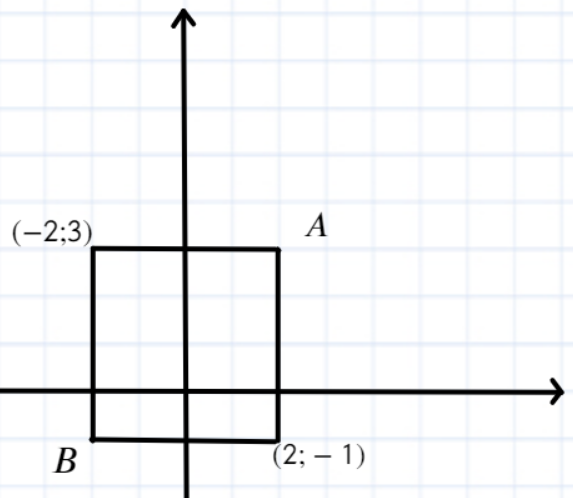
\includegraphics[width=1\linewidth]{kv1.png}
 %% метка рисунка для ссылки на него
\end{minipage}
\hfill
\begin{minipage}[h]{0.4\linewidth}
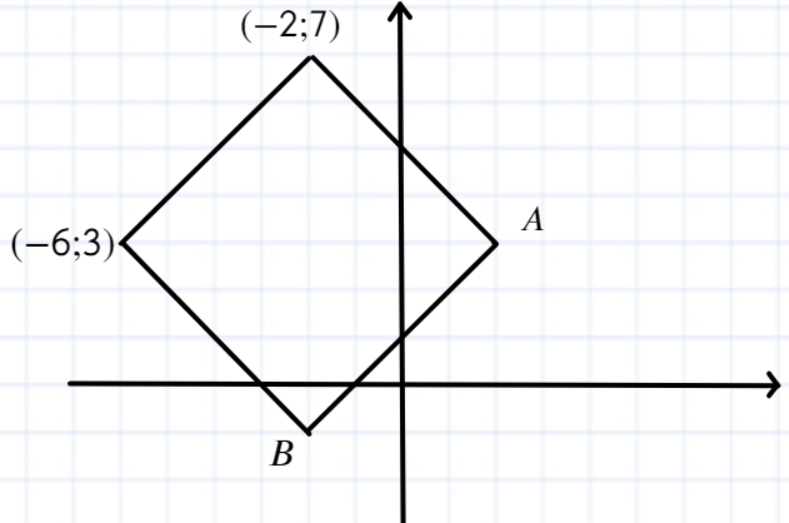
\includegraphics[width=1\linewidth]{kv2.png}
\end{minipage}
\hfill
\begin{minipage}[h]{0.2\linewidth}
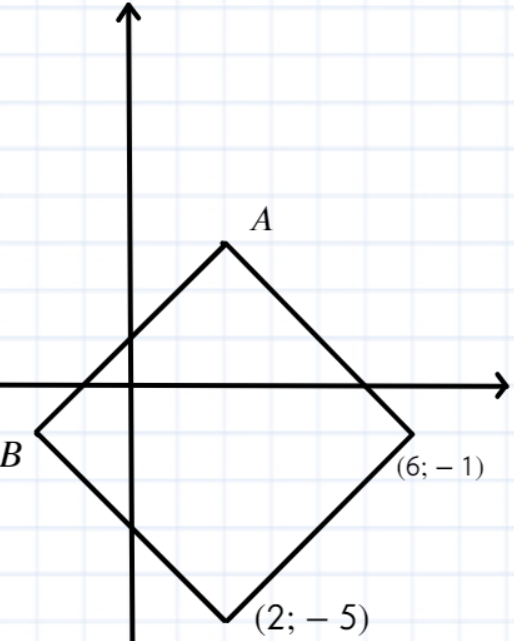
\includegraphics[width=1\linewidth]{kv3.png}
 %% метка рисунка для ссылки на него
\end{minipage}
\hfill
\end{center}
\end{figure}\\
57. Найдём точку, в которой прямая $y=-0,5x+4$ пересекает ось $Ox$ (в ней $y=0):\ 0=-0,5x+4,\ x=8$ и ось $Oy$ (в ней $x=0):\ y=-0,5\cdot0+4=4.$ Если $BA$ является медианой, точка $A$ лежит посередине между $O$ и $C,$ а значит точка $C$ имеет координаты $(0;8).$ Проведём прямую через неё и точку $B(8;0):\
\begin{cases} 8=0+b,\\ 0=8k+b.\end{cases}\Rightarrow y=-x+8.$
$$\begin{tikzpicture}[scale=0.2]
\tikzset {line01/.style={line width =0.5pt}}
\tikzset{line02/.style={line width =1pt}}
\tikzset{line03/.style={dashed,line width =0.5pt}}
%\filldraw [black] (0,0) circle (1pt);
\draw [->] (-10,0) -- (10,0);
\draw [->] (0,-10) -- (0,10);
\draw[line01] (9,-1) -- (-1,9);
%\draw[line03] (-1,1) -- (0,1);
%\draw[line03] (-1,0) -- (-1,1);
%\draw[line01] (0,-3) -- (-2,5);
%\draw (0.6,-4) node {\tiny $-4$};
%\draw (-1.6,-0.7) node {\tiny $-1$};
\draw (10.2,0.7) node {\scriptsize $x$};
\draw (0.5,8) node {\tiny $8$};
\draw (8,0.5) node {\tiny $8$};
\draw (0.7,10.2) node {\scriptsize $y$};
\end{tikzpicture}$$
58. $y=(x^2-4)\left(\cfrac{1}{x-2}-\cfrac{1}{x+2}\right)-x=(x-2)(x+2)\cdot\cfrac{x+2-x+2}{(x-2)(x+2)}-x=4-x,$ при этом $x\neq\pm2.$ Проведём прямую через точки $(0;4)$ и $(4;0),$ не забыв выколоть точки $(-2;6)$ и $(2;2).$
$$\begin{tikzpicture}[scale=0.2]
\tikzset {line01/.style={line width =0.5pt}}
\tikzset{line02/.style={line width =1pt}}
\tikzset{line03/.style={dashed,line width =0.5pt}}
%\filldraw [black] (0,0) circle (1pt);
\draw [->] (-10,0) -- (10,0);
\draw [->] (0,-10) -- (0,10);
\draw[line01] (-6,10) -- (8,-4);
\draw (10.2,0.7) node {\scriptsize $x$};
\draw (-2.5,-0.7) node {\scriptsize $-2$};
\draw (2,-0.7) node {\scriptsize $2$};
\draw (-0.7,2) node {\scriptsize $2$};
\draw (0.7,6) node {\scriptsize $6$};
%\draw (-5.5,-2) node {\scriptsize $-6$};
\draw[line03] (-2,0) -- (-2,6);
\draw[line03] (0,6) -- (-2,6);
\draw[line03] (2,0) -- (2,2);
\draw[line03] (0,2) -- (2,2);
\draw (0.7,10.2) node {\scriptsize $y$};
\draw (2,2) circle (10pt);
\draw (-2,6) circle (10pt);
\end{tikzpicture}$$
59. $y=\cfrac{|x|}{x}\left(-\cfrac{1}{2}x+2\right)=\left[\begin{array}{l}\cfrac{1}{2}x-2, x<0,\\ -\cfrac{1}{2}x+2, x>0.\end{array}\right.$
Проведём прямые через точки $(-4;-4)$ и $(0;-2)$ и $(0;2)$ и $(4;0),$ не забыв выколоть точки $(0;-2)$ и $(0;2).$
$$\begin{tikzpicture}[scale=0.2]
\tikzset {line01/.style={line width =0.5pt}}
\tikzset{line02/.style={line width =1pt}}
\tikzset{line03/.style={dashed,line width =0.5pt}}
%\filldraw [black] (0,0) circle (1pt);
\draw [->] (-10,0) -- (10,0);
\draw [->] (0,-10) -- (0,10);
\draw[line01] (0,2) -- (8,-2);
\draw[line01] (0,-2) -- (-8,-6);
\draw (10.2,0.7) node {\scriptsize $x$};
\draw (4,0.7) node {\scriptsize $4$};
\draw (-4,0.7) node {\scriptsize $-4$};
\draw (-1,2) node {\scriptsize $2$};
\draw (1.4,-2) node {\scriptsize $-2$};
\draw (1.2,-4) node {\scriptsize $-4$};
\draw (0.7,10.2) node {\scriptsize $y$};
\draw (0,2) circle (10pt);
\draw (0,-2) circle (10pt);
\draw[line03] (-4,0) -- (-4,-4);
\draw[line03] (0,-4) -- (-4,-4);
\end{tikzpicture}$$
60. $\cfrac{(y^2-4)(y+2x-1)}{x-1}=0\Leftrightarrow\cfrac{(y-2)(y+2)(y-(1-2x))}{x-1}=0\Leftrightarrow\begin{cases}
\left[\begin{array}{l} y=2,\\ y=-2, \\ y=1-2x.\end{array}\right.\\ x\neq1.\end{cases}$
$$\begin{tikzpicture}[scale=0.2]
\tikzset {line01/.style={line width =0.5pt}}
\tikzset{line02/.style={line width =1pt}}
\tikzset{line03/.style={dashed,line width =0.5pt}}
%\filldraw [black] (0,0) circle (1pt);
\draw [->] (-10,0) -- (10,0);
\draw [->] (0,-10) -- (0,10);
\draw[line01] (-9,2) -- (9,2);
\draw[line01] (-9,-2) -- (9,-2);
\draw[line01] (5,-9) -- (-4,9);
\draw[line03] (1,2) -- (1,-2);
\draw[line03] (0,-1) -- (1,-1);
\draw[line03] (-3,0) -- (-3,7);
\draw[line03] (0,7) -- (-3,7);
\draw (1.5,0.5) node {\tiny $1$};
\draw (-3.2,-0.7) node {\tiny $-3$};
\draw (0.5,7) node {\tiny $7$};
\draw (0.5,2.7) node {\tiny $2$};
\draw (-1,-2.7) node {\tiny $-2$};
\draw (-1,-1) node {\tiny $-1$};
\draw (10.2,0.7) node {\scriptsize $x$};
\draw (-0.7,10.2) node {\scriptsize $y$};
\draw (1,2) circle (7pt);
\draw (1,-2) circle (7pt);
\draw (1,-1) circle (7pt);
\end{tikzpicture}$$
61. Приведём пример одной из возможных кусочно-линейных функций и нарисуем её график:
$$y=\begin{cases} 0,\ 0<x\leqslant\cfrac{1}{3},\\
3x-1,\ \cfrac{1}{3}<x\leqslant\cfrac{2}{3},\\
1,\ \cfrac{2}{3}<x<1.\end{cases}$$
$$\begin{tikzpicture}[scale=0.4]
\tikzset {line01/.style={line width =1pt}}
\tikzset{line02/.style={line width =1pt}}
\tikzset{line03/.style={dashed,line width =0.5pt}}
%\filldraw [black] (0,0) circle (1pt);
\draw [->] (-6,0) -- (10,0);
\draw [->] (0,-6) -- (0,10);
\draw[line01] (0,0) -- (1,0);
\draw[line01] (1,0) -- (2,3);
\draw[line01] (2,3) -- (3,3);
\draw (3,-0.5) node {\tiny $1$};
\draw (-0.5,3) node {\tiny $1$};
\draw (0,0) circle (10pt);
\draw (3,3) circle (10pt);
\draw (10.2,0.7) node {\scriptsize $x$};
\draw (-0.7,10.2) node {\scriptsize $y$};
\draw[line03] (0,3) -- (3,3);
\draw[line03] (3,0) -- (3,3);
\end{tikzpicture}
$$
62. Подставим в уравнение данной функции точку $(0;0):\ 0=\cfrac{5a}{a-5}\cdot(0-1)+\cfrac{a^2}{a-5},\ 0=\cfrac{a^2-5a}{a-5}=\cfrac{a(a-5)}{a-5}=0,\ a=0.$\\
63. У точек на оси абсцисс координата $y=0,$ подставим значения $x$ и $y$ в уравнение графика функции:
$0=\cfrac{-\cfrac{4}{3}-b}{3\cdot\left(-\cfrac{4}{3}\right)+1}+b\cdot\left(-\cfrac{4}{3}\right),\ \cfrac{4}{3}+b-4b=0,\ b=\cfrac{4}{9}.$\\
64. $y=(2-0,5x): (-0,125)=4x-16.$ У этих функций одинаковый коэффициент $k,$ значит они не пересекаются. Оси они пересекают в точках $(0;-16),\ (4;0),\ (0;-1),\ \left(\cfrac{1}{4};0\right).$
$$\begin{tikzpicture}[scale=0.2]
\tikzset {line01/.style={line width =0.5pt}}
\tikzset{line02/.style={line width =1pt}}
\tikzset{line03/.style={dashed,line width =0.5pt}}
%\filldraw [black] (0,0) circle (1pt);
\draw [->] (-5,0) -- (10,0);
\draw [->] (0,-20) -- (0,11);
\draw[line01] (-1,-20) -- (6,8);
\draw[line01] (-1,-5) -- (3,11);
%\draw[line03] (-1,1) -- (0,1);
%\draw[line03] (-1,0) -- (-1,1);
%\draw[line01] (0,-3) -- (-2,5);
%\draw (0.6,-4) node {\tiny $-4$};
%\draw (-1.6,-0.7) node {\tiny $-1$};
\draw (10.2,0.7) node {\scriptsize $x$};
\draw (4.3,-1) node {\tiny $4$};
\draw (0.5,-1) node {\tiny $\frac{1}{4}$};
\draw (-1,-1) node {\tiny $-1$};
\draw (-1.5,-16) node {\tiny $-16$};
\draw (0.7,11.2) node {\scriptsize $y$};
\end{tikzpicture}$$
65. Найдём точку пересечения прямых $y=\cfrac{1}{3}x-2$ и $y=6-x:\ \cfrac{1}{3}x-2=6-x,\ \cfrac{4}{3}x=8,\ x=6,\ y=6-x=0.$ Прямая $y=-4x-3$ пересекает ось $Oy$ в точке с абсциссой $x=0$ и ординатой $y=0-3=-3.$ Найдём прямую, проходящую через полученные точки: $\begin{cases} 6k+b=0,\\ 0+b=-3.\end{cases}\Leftrightarrow
\begin{cases} k=\cfrac{1}{2},\\ b=-3.\end{cases}$ Проведём прямую через две точки $(0;-3)$ и $(6;0).$
$$\begin{tikzpicture}[scale=0.2]
\tikzset {line01/.style={line width =0.5pt}}
\tikzset{line02/.style={line width =1pt}}
\tikzset{line03/.style={dashed,line width =0.5pt}}
%\filldraw [black] (0,0) circle (1pt);
\draw [->] (-6.5,0) -- (10,0);
\draw [->] (0,-10) -- (0,10);
\draw[line01] (8,1) -- (-6,-6);
%\draw[line03] (-1,1) -- (0,1);
%\draw[line03] (-1,0) -- (-1,1);
%\draw[line01] (0,-3) -- (-2,5);
%\draw (0.6,-4) node {\tiny $-4$};
%\draw (-1.6,-0.7) node {\tiny $-1$};
\draw (10.2,0.7) node {\scriptsize $x$};
\draw (1,-3) node {\tiny $-3$};
\draw (6,-0.5) node {\tiny $6$};
\draw (0.7,10.2) node {\scriptsize $y$};
\end{tikzpicture}$$
66. а) Проведём прямую через две точки $(-1;1)$ и $(0;3).$
$$\begin{tikzpicture}[scale=0.2]
\tikzset {line01/.style={line width =0.5pt}}
\tikzset{line02/.style={line width =1pt}}
\tikzset{line03/.style={dashed,line width =0.5pt}}
%\filldraw [black] (0,0) circle (1pt);
\draw [->] (-6.5,0) -- (10,0);
\draw [->] (0,-10) -- (0,10);
\draw[line01] (-4,-5) -- (3,9);
\draw[line03] (-1,1) -- (0,1);
\draw[line03] (-1,0) -- (-1,1);
%\draw[line01] (0,-3) -- (-2,5);
%\draw (0.6,-4) node {\tiny $-4$};
%\draw (-1.6,-0.7) node {\tiny $-1$};
\draw (10.2,0.7) node {\scriptsize $x$};
\draw (0.5,3) node {\tiny $3$};
\draw (0.5,1) node {\tiny $1$};
\draw (-1.5,-1) node {\tiny $-1$};
\draw (0.7,10.2) node {\scriptsize $y$};
\end{tikzpicture}$$
б) Подставим координаты точки $A$ в уравнение прямой: $1=k\cdot(-1)+3,\ k=2.$\\
в) Ось абсцисс эта прямая пересекает в точке $\left(-\cfrac{3}{2};0\right)$ и образует прямоугольный треугольник с катетами $\cfrac{3}{2}$ и $3.$ Его площадь равна $\cfrac{1}{2}\cdot\cfrac{3}{2}\cdot3=\cfrac{9}{4}.$\\
г) Так как угловые коэффициенты у этих прямых разные, они пересекаются.\\
67. а) Это прямоугольник, ограниченный прямыми $x=3,\ x=9,\ y=-3,\ y=6.$
$$\begin{tikzpicture}[scale=0.2]
\tikzset {line01/.style={line width =0.5pt}}
\tikzset{line02/.style={line width =1pt}}
\tikzset{line03/.style={dashed,line width =0.5pt}}
%\filldraw [black] (0,0) circle (1pt);
\draw [->] (-10,0) -- (12,0);
\draw [->] (0,-10) -- (0,10);
\filldraw [draw=black] (3,-3) rectangle (9,6);
\draw[line03] (0,-3) -- (3,-3);
\draw[line03] (0,6) -- (3,6);
%\draw[line03] (-1,0) -- (-1,1);
%\draw[line01] (0,-3) -- (-2,5);
%\draw (0.6,-4) node {\tiny $-4$};
%\draw (-1.6,-0.7) node {\tiny $-1$};
\draw (12.2,0.7) node {\scriptsize $x$};
\draw (2.6,0.5) node {\tiny $3$};
\draw (-0.9,-3) node {\tiny $-3$};
\draw (-0.6,6) node {\tiny $6$};
\draw (9.4,0.5) node {\tiny $9$};
%\draw (-2.2,1) node {\tiny $-\frac{3}{2}$};
\draw (0.7,10.2) node {\scriptsize $y$};
\end{tikzpicture}$$
б) Горизонтальная сторона этого прямоугольника равна $a+6-a=6,$ а вертикальная --- $2a-(-a)=3a.$ Он является квадратом при $3a=6,\ a=2.$\\
68. Построим каждую из прямых по двум точкам, отмеченным на рисунке (они найдены как точки пересечения данных прямых).
$$\begin{tikzpicture}[scale=0.2]
\tikzset {line01/.style={line width =0.5pt}}
\tikzset{line02/.style={line width =1pt}}
\tikzset{line03/.style={dashed,line width =0.5pt}}
%\filldraw [black] (0,0) circle (1pt);
\draw [->] (-5,0) -- (20,0);
\draw [->] (0,-5) -- (0,5);
\draw[line02] (18,2.5) -- (-0.833,2.5);
\draw[line02] (18,2.5) -- (0.615,-1.846);
\draw[line02] (0.615,-1.846) -- (-0.833,2.5);
\draw (20.2,0.7) node {\scriptsize $x$};
\draw (-3.5,2.5) node {\scriptsize $(-\frac{5}{6};\frac{5}{2})$};
\draw (3.5,-3) node {\scriptsize $(\frac{8}{13};-\frac{24}{13})$};
\draw (18.5,4) node {\scriptsize $(18;\frac{5}{2})$};
\draw (0.7,5.2) node {\scriptsize $y$};
\end{tikzpicture}$$
69. Найдём прямую, проходящую через точки $M(2;-5)$ и $N(0;-2): \begin{cases} 2k+b=-5,\\ b=-2.\end{cases}\Leftrightarrow\begin{cases} k=-\cfrac{3}{2},\\ b=-2.\end{cases}$ Приведём уравнение этой прямой к искомому виду: $y=-\cfrac{3}{2}x-2,\ 2y=-3x-4,\ 3x+2y=-4.$\\
70. Построим квадрат с вершинами $(-1;5),\ (-1;1),\ (3;5)$ и $(3;1).$ Тогда прямая $y=x+2$ является его диагональю и вершине $A(3;1)$ относительно диагонали симметрична вершина $(-1;5).$\\
71. а) $\cfrac{x}{x^2+2x+4}+\cfrac{x^2+8}{x^3-8}-\cfrac{1}{x-2}=\cfrac{x}{x^2+2x+4}+\cfrac{x^2+8}{(x-2)(x^2+2x+4)}-\cfrac{1}{x-2}=$\\$
\cfrac{x^2-2x+x^2+8-x^2-2x-4}{(x-2)(x^2+2x+4)}=\cfrac{x^2-4x+4}{(x-2)(x^2+2x+4)}=\cfrac{(x-2)^2}{(x-2)(x^2+2x+4)}=\cfrac{x-2}{x^2+2x+4}.$\\
$\cfrac{x^2}{x^2-4}-\cfrac{2}{2-x}=\cfrac{x^2}{(x-2)(x+2)}+\cfrac{2}{x-2}=\cfrac{x^2+2x+4}{(x-2)(x+2)}.$\\
$\cfrac{x-2}{x^2+2x+4}\cdot\cfrac{x^2+2x+4}{(x-2)(x+2)}=\cfrac{1}{x+2}.$\\
б) $y=\cfrac{1}{f(x)}=x+2,$ при этом нельзя брать $x=\pm2,$ так как эти значения обнуляли знаменатель.
$$\begin{tikzpicture}[scale=0.2]
\tikzset {line01/.style={line width =0.5pt}}
\tikzset{line02/.style={line width =1pt}}
\tikzset{line03/.style={dashed,line width =0.5pt}}
%\filldraw [black] (0,0) circle (1pt);
\draw [->] (-10,0) -- (10,0);
\draw [->] (0,-10) -- (0,10);
\draw[line01] (-6,-4) -- (8,10);
\draw (10.2,0.7) node {\scriptsize $x$};
\draw (-1.9,-1.5) node {\scriptsize $-2$};
\draw (2,-0.7) node {\scriptsize $2$};
\draw (-0.7,4) node {\scriptsize $4$};
%\draw (0.7,6) node {\scriptsize $6$};
%\draw (-5.5,-2) node {\scriptsize $-6$};
\draw[line03] (2,0) -- (2,4);
\draw[line03] (0,4) -- (2,4);
\draw (0.7,10.2) node {\scriptsize $y$};
\draw (2,4) circle (10pt);
\draw (-2,0) circle (10pt);
\end{tikzpicture}$$
72. а) Найдём прямую $AB:\ \begin{cases} b=-7,\\ 3k+b=2.\end{cases}\Leftrightarrow\begin{cases} b=-7,\\ k=3.\end{cases}\Rightarrow y=3x-7.$
Найдём прямую $CD:\ \begin{cases} k+b=1,\\ -30k+b=63.\end{cases}\Leftrightarrow\begin{cases} 31k=-62,\\ -30k+b=63.\end{cases}
\Leftrightarrow\begin{cases} k=-2,\\ b=3.\end{cases}\Rightarrow y=-2x+3.$\\
б) Найдём точку пересечения прямых $AB$ и $CD: 3x-7=-2x+3,\ 5x=10,\ x=2,\ y=3\cdot2-7=-1.$ Найдём прямую $BC:\ \begin{cases} 3k+b=2,\\ k+b=1.\end{cases}\Leftrightarrow\begin{cases} 2k=1,\\ k+b=1.\end{cases}\Leftrightarrow\begin{cases} k=\cfrac{1}{2},\\ b=\cfrac{1}{2}.\end{cases}\Rightarrow y=\cfrac{1}{2}x+\cfrac{1}{2}.$ Точка этой прямой, лежащая на оси абсцисс, имеет ординату $y=0,$ а значит $\cfrac{1}{2}x+\cfrac{1}{2}=0,\ x=-1.$ Таким образом, необходимо найти уравнение прямой, проходящей через точки $(2;-1)$ и $(-1;0): \ \begin{cases} 2k+b=-1,\\ -k+b=0.\end{cases}\Leftrightarrow\begin{cases} 3k=-1,\\ -k+b=0.\end{cases}\Leftrightarrow\begin{cases} k=-\cfrac{1}{3},\\ b=-\cfrac{1}{3}.\end{cases}\Rightarrow y=-\cfrac{1}{3}x-\cfrac{1}{3}.$\\
73. а) Найдём прямую $AC:\ \begin{cases} b=4,\\ -3k+b=-2.\end{cases}\Leftrightarrow\begin{cases} b=4,\\ k=2.\end{cases}\Rightarrow y=2x+4.$
Найдём прямую $BD:\ \begin{cases} k+b=-4,\\ -20k+b=59.\end{cases}\Leftrightarrow\begin{cases} 21k=-63,\\ -20k+b=59.\end{cases}
\Leftrightarrow\begin{cases} k=-3,\\ b=-1.\end{cases}\Rightarrow y=-3x-1.$\\
б) Найдём точку пересечения прямых $AC$ и $BD: 2x+4=-3x-1,\ 5x=-5,\ x=-1,\ y=2\cdot(-1)+4=2.$ Найдём прямую $BC:\ \begin{cases} k+b=-4,\\ -3k+b=-2.\end{cases}\Leftrightarrow\begin{cases} 4k=-2,\\ -3k+b=-2.\end{cases}\Leftrightarrow\begin{cases} k=-\cfrac{1}{2},\\ b=-\cfrac{7}{2}.\end{cases}\Rightarrow y=-\cfrac{1}{2}x-\cfrac{7}{2}.$ Точка этой прямой, лежащая на оси абсцисс, имеет ординату $y=0,$ а значит $-\cfrac{1}{2}x-\cfrac{7}{2}=0,\ x=-7.$ Таким образом, необходимо найти уравнение прямой, проходящей через точки $(-1;2)$ и $(-7;0): \ \begin{cases} -k+b=2,\\ -7k+b=0.\end{cases}\Leftrightarrow\begin{cases} 6k=2,\\ -7k+b=0.\end{cases}\Leftrightarrow\begin{cases} k=\cfrac{1}{3},\\ b=\cfrac{7}{3}.\end{cases}\Rightarrow y=\cfrac{1}{3}x+\cfrac{7}{3}.$\\
74. а) Построим график по двум точкам $(0;4)$ и $(2;0).$
$$\begin{tikzpicture}[scale=0.2]
\tikzset {line01/.style={line width =0.5pt}}
\tikzset{line02/.style={line width =1pt}}
\tikzset{line03/.style={dashed,line width =0.5pt}}
%\filldraw [black] (0,0) circle (1pt);
\draw [->] (-10,0) -- (10,0);
\draw [->] (0,-10) -- (0,10);
\draw[line01] (-2,8) -- (5,-6);
%\draw[line03] (-1,1) -- (0,1);
%\draw[line03] (-1,0) -- (-1,1);
%\draw[line01] (0,-3) -- (-2,5);
%\draw (0.6,-4) node {\tiny $-4$};
%\draw (-1.6,-0.7) node {\tiny $-1$};
\draw (10.2,0.7) node {\scriptsize $x$};
\draw (0.7,4) node {\tiny $4$};
\draw (2,0.9) node {\tiny $2$};
\draw (0.7,10.2) node {\scriptsize $y$};
\end{tikzpicture}$$
б) Найдём точку пересечения прямых $y=x+2$ и $2x+3y-16=0:\ \begin{cases}y=x+2,\\ 2x+3y-16=0. \end{cases}\Leftrightarrow
\begin{cases}y=x+2,\\ 2x+3x+6-16=0. \end{cases}\Leftrightarrow
\begin{cases}y=4,\\ x=2. \end{cases}$ Расстояние от точки $(2;0)$ до точки $(2;4)$ равно 4.\\
75. а) Построим график по двум точкам $(0;6)$ и $(3;0).$
$$\begin{tikzpicture}[scale=0.2]
\tikzset {line01/.style={line width =0.5pt}}
\tikzset{line02/.style={line width =1pt}}
\tikzset{line03/.style={dashed,line width =0.5pt}}
%\filldraw [black] (0,0) circle (1pt);
\draw [->] (-10,0) -- (10,0);
\draw [->] (0,-10) -- (0,10);
\draw[line01] (-2,10) -- (5,-4);
%\draw[line03] (-1,1) -- (0,1);
%\draw[line03] (-1,0) -- (-1,1);
%\draw[line01] (0,-3) -- (-2,5);
%\draw (0.6,-4) node {\tiny $-4$};
%\draw (-1.6,-0.7) node {\tiny $-1$};
\draw (10.2,0.7) node {\scriptsize $x$};
\draw (0.7,6) node {\tiny $6$};
\draw (3,0.9) node {\tiny $3$};
\draw (0.7,10.2) node {\scriptsize $y$};
\end{tikzpicture}$$
б) Найдём точку пересечения прямых $y=x+3$ и $x-2y+9=0:\ \begin{cases}y=x+3,\\ x-2y+9=0. \end{cases}\Leftrightarrow
\begin{cases}y=x+3,\\ x-2x-6+9=0. \end{cases}\Leftrightarrow
\begin{cases}y=6,\\ x=3. \end{cases}$ Расстояние от точки $(3;0)$ до точки $(3;6)$ равно 6.\\
76. Найдём ординату точки $A:\ (-2)\cdot0+2=2,$ значит она имеет координаты $(0;2).$ Найдём абсциссу точки $B:\ 0=-2x+2,\ x=1,$ значит она имеет координаты $(1;0).$ Тогда середина стороны $OB$ имеет координаты $M\left(\cfrac{1}{2};0\right).$ Проведём прямую $y=kx+b$ через точки $A$ и $M:\ \begin{cases} b=2,\\ \cfrac{1}{2}k+b=0.\end{cases}\Leftrightarrow\begin{cases} b=2,\\ k=-4.\end{cases}\Rightarrow y=-4x+2.$\\
77. Найдём ординату точки $A:\ 2\cdot0+2=2,$ значит она имеет координаты $(0;2).$ Найдём абсциссу точки $B:\ 0=2x+2,\ x=-1,$ значит она имеет координаты $(-1;0).$ Тогда середина стороны $OB$ имеет координаты $M\left(-\cfrac{1}{2};0\right).$ Проведём прямую $y=kx+b$ через точки $A$ и $M:\ \begin{cases} b=2,\\ -\cfrac{1}{2}k+b=0.\end{cases}\Leftrightarrow\begin{cases} b=2,\\ k=4.\end{cases}\Rightarrow y=4x+2.$\\
78. Так как сумма координат точки $M$ равна 6, получим систему уравнений $\begin{cases} y=6-x,\\ y=x+8.\end{cases}\Rightarrow 6-x=x+8,\ -2x=2,\ x=-1,\ y=6+1=7.$ Тогда $7=(2a-1)\cdot(-1)+a+3,\ 7=-2a+1+a+3,\ a=-3.$\\
79. Найдём точку пересечения прямых $y=2x-3$ и $y=-x-6:\ 2x-3=-x-6,\ 3x=-3,\ x=-1,\ y=1-6=-5.$ Тогда $-5=-a-a-2,\ 2a=3,\ a=\cfrac{3}{2}.$\\
80. Так как сумма координат точки $A$ равна 4, получим систему уравнений $\begin{cases} y=4-x,\\ y=x+6.\end{cases}\Rightarrow 4-x=x+6,\ -2x=2,\ x=-1,\ y=4+1=5.$ Тогда $5=(2a+1)\cdot(-1)+a+4,\ 5=-2a-1+a+4,\ a=-2.$\\
81. Найдём точку пересечения прямых $y=3x-4$ и $y=-2x+1:\ 3x-4=-2x+1,\ 5x=5,\ x=1,\ y=3-4=-1.$ Тогда $-1=a-1+2a-3,\ 3a=3,\ a=1.$\\
82. $\cfrac{((x^2-4)^2+y^2-2y+1)(y^2-3xy+2x^2)}{xy-2y+3x-6}=0\Leftrightarrow
\begin{cases}

((x^2-4)^2+y^2-2y+1)(y^2-3xy+2x^2)=0,\\
xy-2y+3x-6\neq0.
\end{cases}$\\$\Leftrightarrow
\begin{cases}
\left[\begin{array}{l}
(x^2-4)^2+(y-1)^2=0,\\
y(y-x)+2x(x-y)=0,
\end{array}\right.\\
y(x-2)+3(x-2)\neq0.
\end{cases}\Leftrightarrow
\begin{cases}
\left[\begin{array}{l}
\begin{cases}
x^2-4=0,\\
y-1=0.
\end{cases}\\
(y-x)(y-2x)=0,
\end{array}\right.\\
(x-2)(y+3)\neq0.
\end{cases}\Leftrightarrow
\begin{cases}
\left[\begin{array}{l}
\begin{cases}
x=2,\\
y=1.
\end{cases}\\
\begin{cases}
x=-2,\\
y=1.
\end{cases}\\
y=x,\\
y=2x,
\end{array}\right.\\
x\neq2,\\
y\neq-3.
\end{cases}$
\begin{figure}[ht!]
\center{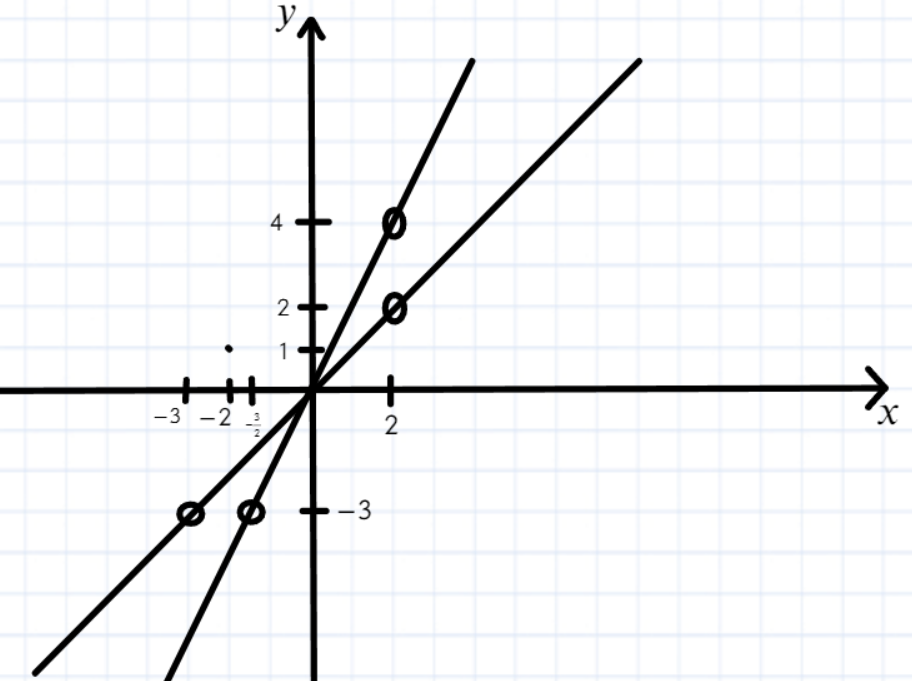
\includegraphics[scale=0.35]{gr7-82.png}}
\end{figure}\newpage\noindent
83. $\cfrac{((x^2-4)^2+y^2+2y+1)(y^2-4xy+3x^2)}{xy-2y+2x-4}=0\Leftrightarrow
\begin{cases}
((x^2-4)^2+y^2+2y+1)(y^2-4xy+3x^2)=0,\\
xy-2y+2x-4\neq0.
\end{cases}$\\$\Leftrightarrow
\begin{cases}
\left[\begin{array}{l}
(x^2-4)^2+(y+1)^2=0,\\
y(y-x)+3x(x-y)=0,
\end{array}\right.\\
y(x-2)+2(x-2)\neq0.
\end{cases}\Leftrightarrow
\begin{cases}
\left[\begin{array}{l}
\begin{cases}
x^2-4=0,\\
y+1=0.
\end{cases}\\
(y-x)(y-3x)=0,
\end{array}\right.\\
(x-2)(y+2)\neq0.
\end{cases}\Leftrightarrow
\begin{cases}
\left[\begin{array}{l}
\begin{cases}
x=2,\\
y=-1.
\end{cases}\\
\begin{cases}
x=-2,\\
y=-1.
\end{cases}\\
y=x,\\
y=3x,
\end{array}\right.\\
x\neq2,\\
y\neq-2.
\end{cases}$
\begin{figure}[ht!]
\center{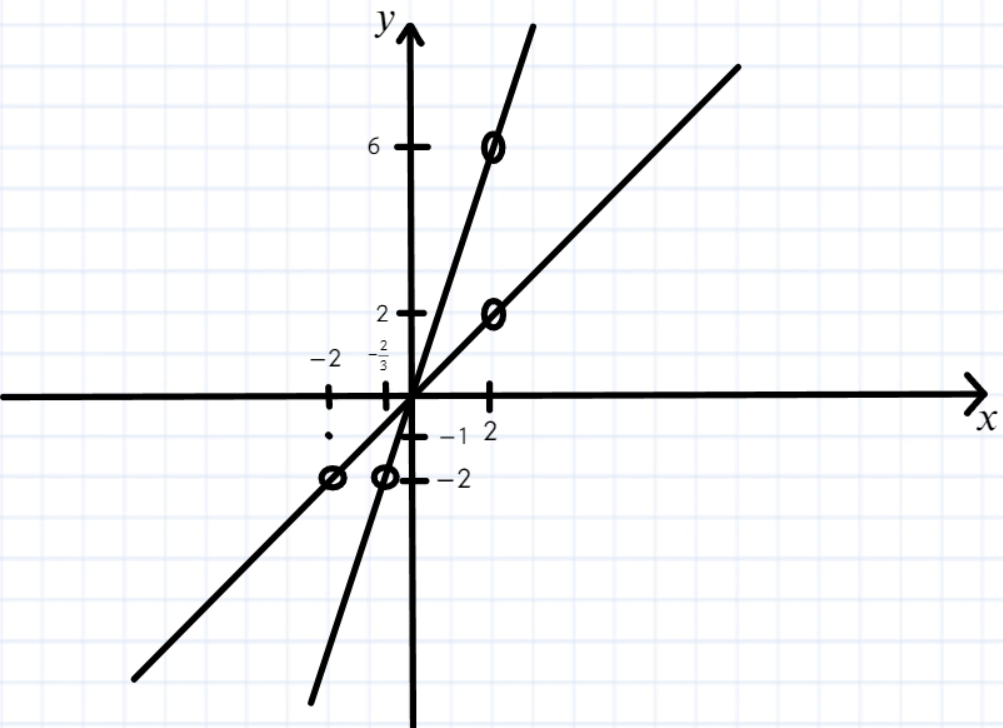
\includegraphics[scale=0.35]{gr7-83.png}}
\end{figure}\\
84. а) $y=\cfrac{x^2-2x}{2-x}+4=\cfrac{x(x-2)}{2-x}+4=\begin{cases} 4-x,\\ x\neq 2.\end{cases}$\\
\begin{figure}[ht!]
\center{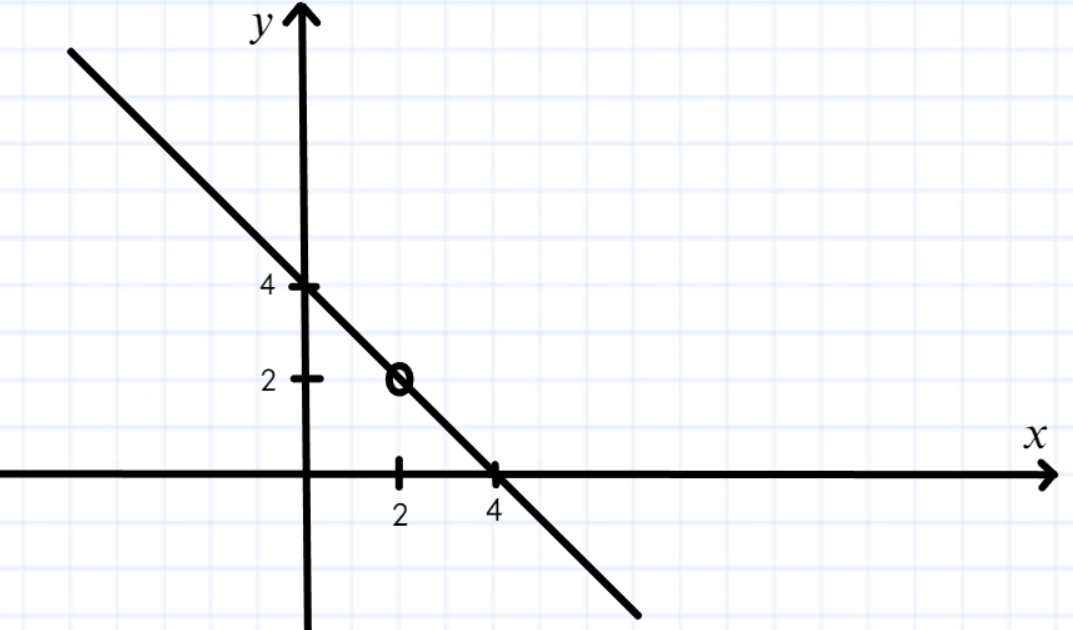
\includegraphics[scale=0.35]{gr7-84.png}}
\end{figure}\\
б) При положительных $x$ функция принимает значения $(-\infty;2)\cup(2;4).$\\
в) Эта прямая не будет иметь общих точек с графиком функции, если она параллельна прямой $y=4-x$ или если она проходит через выколотую точку $(2;2).$ Пусть это прямая $y=kx+b.$ В первом случае её угловой коэффициент равен $-1,$ значит $-1=-1+b,\ b=0,$ то есть это функция $y=-x.$ Во втором случае $\begin{cases} -1=k+b,\\ 2=2k+b.\end{cases}\Leftrightarrow
\begin{cases} -3=-k,\\ b=2-2k.\end{cases}\Leftrightarrow
\begin{cases} k=3,\\ b=-4.\end{cases},$ то есть прямая задана уравнением $y=3x-4.$\newpage\noindent
85. а) $y=\cfrac{x^2-3x}{3-x}+1=\cfrac{x(x-3)}{3-x}+1=\begin{cases} 1-x,\\ x\neq 3.\end{cases}$\\
\begin{figure}[ht!]
\center{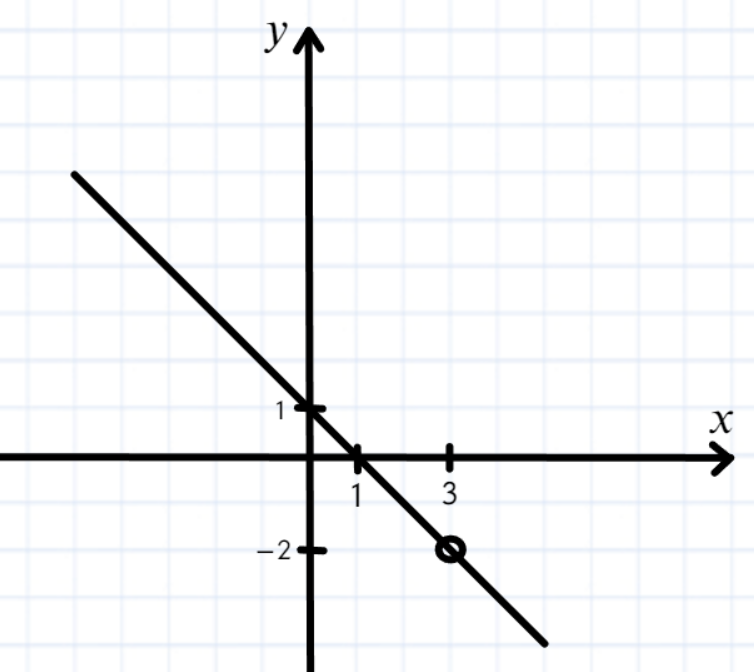
\includegraphics[scale=0.35]{gr7-85.png}}
\end{figure}\\
б) При положительных $x$ функция принимает значения $(-\infty;-2)\cup(-2;1).$\\
в) Эта прямая не будет иметь общих точек с графиком функции, если она параллельна прямой $y=1-x$ или если она проходит через выколотую точку $(3;-2).$ Пусть это прямая $y=kx+b.$ В первом случае её угловой коэффициент равен $-1,$ значит $-1=2+b,\ b=-3,$ то есть это функция $y=-x-3.$ Во втором случае $\begin{cases} -2=3k+b,\\ -1=-2k+b.\end{cases}\Leftrightarrow
\begin{cases} -1=5k,\\ b=2k-1.\end{cases}\Leftrightarrow
\begin{cases} k=-\cfrac{1}{5},\\ b=-\cfrac{7}{5}.\end{cases},$ то есть прямая задана уравнением $y=-\cfrac{1}{5}x-\cfrac{7}{5}.$\\
86. Найдём точку пересечения: $4x+3a=2x+4a,\ 2x=a,\ x=\cfrac{a}{2},\ y=2\cdot\cfrac{a}{2}+4a=5a.$ Если $5a=4,$ то $a=\cfrac{4}{5}.$\\
87. $y=\cfrac{x^2+2x}{|x|}=\cfrac{x(x+2)}{|x|}=\begin{cases} x+2,\ x>0,\\ -x-2,\ x<0.\end{cases}$\\
\begin{figure}[ht!]
\center{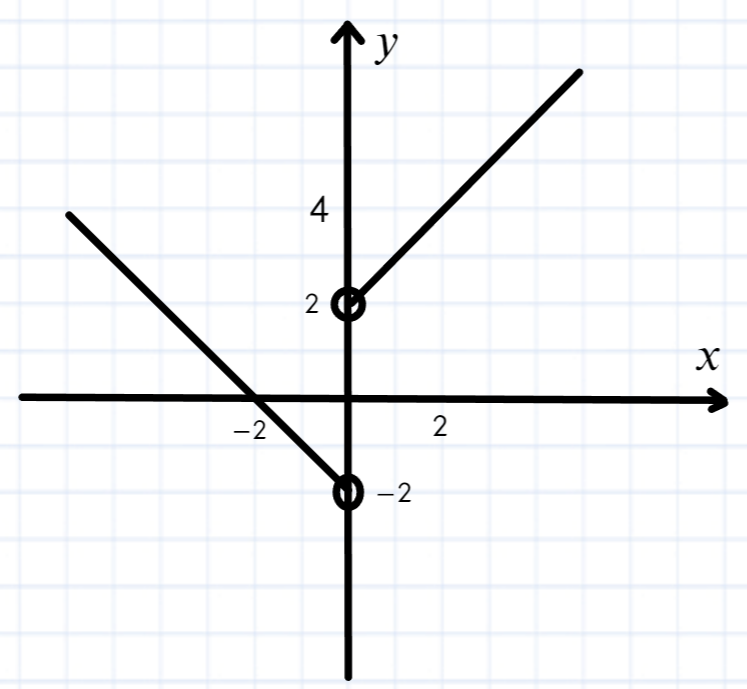
\includegraphics[scale=0.35]{gr7-87.png}}
\end{figure}\newpage\noindent
88. $y=\cfrac{4-x^2}{x+2}-1=\cfrac{(2-x)(2+x)}{x+2}-1=\begin{cases} 1-x,\\ x\neq-2.\end{cases}$\\
\begin{figure}[ht!]
\center{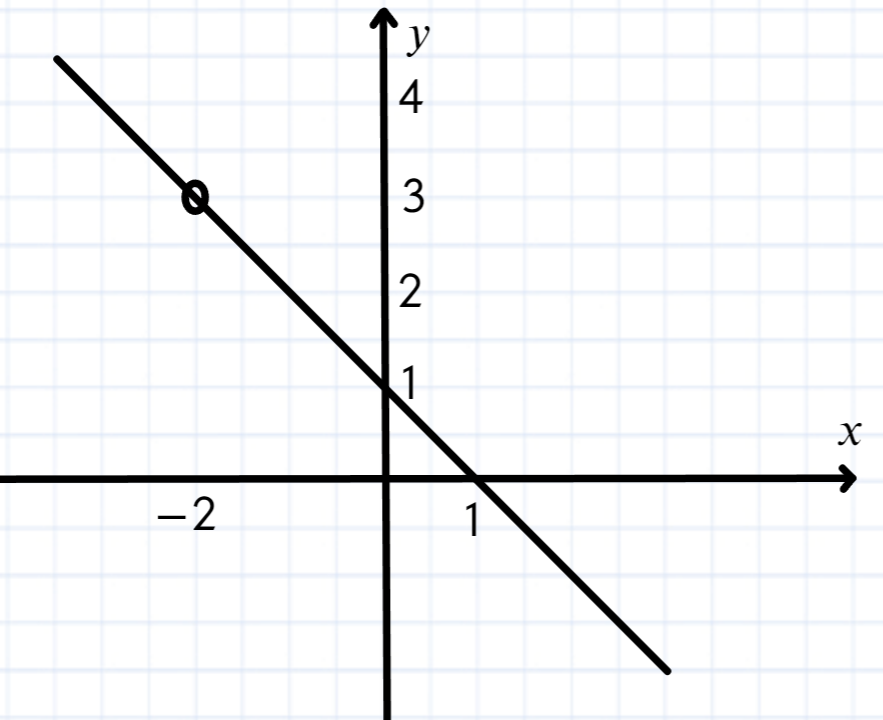
\includegraphics[scale=0.35]{gr7-88.png}}
\end{figure}\\
По графику определим подходящие значения 1, 2 и 4.\\
89. а) Подставим $x=0,$ тогда $y=0+d=d.$ Так как график этой функции пересекает ось ординат ниже оси абсцисс, получаем условие $d<0.$\\
б) Подставим координаты этой точки: $d=k+d,$ откуда $k=0,$ что соответствует горизонтальной прямой. Значит, график функции через эту точку не проходит.\\
90. Расстояние $AB$ всегда равно $(x+1)-(x-3)=4.$ Расстояние $BC$ может быть равно либо $(2x+3)-(x-3)=x+6,$ либо $(x-3)-(2x+3)=-x-6.$ В первом случае $x+6=4,\ x=-2,$ а во втором --- $-x-6=4,\ x=-10.$\\
91. Расстояние $AB$ всегда равно $(x+1)-(x-3)=4.$ Расстояние $AC$ может быть равно либо $(2x+3)-(x+1)=x+2,$ либо $(x+1)-(2x+3)=-x-2.$ В первом случае $x+2=4,\ x=2,$ а во втором --- $-x-2=4,\ x=-6.$\\
92. $y=\cfrac{2x^3+x^2-2x-1}{1-x^2}=\cfrac{x^2(2x+1)-(2x+1)}{1-x^2}=\cfrac{(2x+1)(x^2-1)}{1-x^2}=-2x-1,\ x\neq\pm1.$
$$\begin{tikzpicture}[scale=0.2]
\tikzset {line01/.style={line width =0.5pt}}
\tikzset{line02/.style={line width =1pt}}
\tikzset{line03/.style={dashed,line width =0.5pt}}
%\filldraw [black] (0,0) circle (1pt);
\draw [->] (-10,0) -- (10,0);
\draw [->] (0,-10) -- (0,10);
\draw[line01] (-5,9) -- (4,-9);
\draw (10.2,0.7) node {\scriptsize $x$};
\draw (-1.2,-1.3) node {\scriptsize $-1$};
\draw (1.2,0.7) node {\scriptsize $1$};
\draw (0.4,1) node {\scriptsize $1$};
\draw (-1.1,-3) node {\scriptsize $-3$};
%\draw (0.7,6) node {\scriptsize $6$};
%\draw (-5.5,-2) node {\scriptsize $-6$};
\draw[line03] (-1,0) -- (-1,1);
\draw[line03] (-0.9,1) -- (0,1);
\draw[line03] (1,0) -- (1,-3);
\draw[line03] (1,-3) -- (0,-3);

\draw (0.7,10.2) node {\scriptsize $y$};
\draw (1,-3) circle (10pt);
\draw (-1,1) circle (10pt);
\end{tikzpicture}$$
93. $y=\cfrac{x^3-x^2-x+1}{1-x^2}=\cfrac{x^2(x-1)-(x-1)}{1-x^2}=\cfrac{(x-1)(x^2-1)}{1-x^2}=1-x,\ x\neq\pm1.$
$$\begin{tikzpicture}[scale=0.2]
\tikzset {line01/.style={line width =0.5pt}}
\tikzset{line02/.style={line width =1pt}}
\tikzset{line03/.style={dashed,line width =0.5pt}}
%\filldraw [black] (0,0) circle (1pt);
\draw [->] (-10,0) -- (10,0);
\draw [->] (0,-10) -- (0,10);
\draw[line01] (-7,8) -- (4,-3);
\draw (10.2,0.7) node {\scriptsize $x$};
\draw (-1.2,-1.3) node {\scriptsize $-1$};
\draw (1.2,0.9) node {\scriptsize $1$};
\draw (0.4,2) node {\scriptsize $2$};

%\draw (0.7,6) node {\scriptsize $6$};
%\draw (-5.5,-2) node {\scriptsize $-6$};
\draw[line03] (-1,0) -- (-1,2);
\draw[line03] (-0.9,2) -- (0,2);


\draw (0.7,10.2) node {\scriptsize $y$};
\draw (1,0) circle (10pt);
\draw (-1,2) circle (10pt);
\end{tikzpicture}$$\\
94. $\cfrac{(4+x(2y-x)-y^2)(x^2+y^2-2(x+y-1))}{3x+y+xy+3}=0\Leftrightarrow$\\$
\begin{cases}

(4+x(2y-x)-y^2)(x^2+y^2-2(x+y-1))=0,\\
3x+y+xy+3\neq0.
\end{cases}\Leftrightarrow$\\$
\begin{cases}
\left[\begin{array}{l}
4+2xy-x^2-y^2=0,\\
x^2+y^2-2x-2y+2=0.
\end{array}\right.\\
x(y+3)+y+3\neq0.
\end{cases}\Leftrightarrow
\begin{cases}
\left[\begin{array}{l}
4=(y-x)^2,\\
(x-1)^2+(y-1)^2=0.
\end{array}\right.\\
(x+1)(y+3)\neq0.
\end{cases}\Leftrightarrow
\begin{cases}
\left[\begin{array}{l}
\begin{cases}
x=1,\\
y=1.
\end{cases}\\
y=2+x,\\
y=-2+x,
\end{array}\right.\\
x\neq-1,\\
y\neq-3.
\end{cases}$
\begin{figure}[ht!]
\center{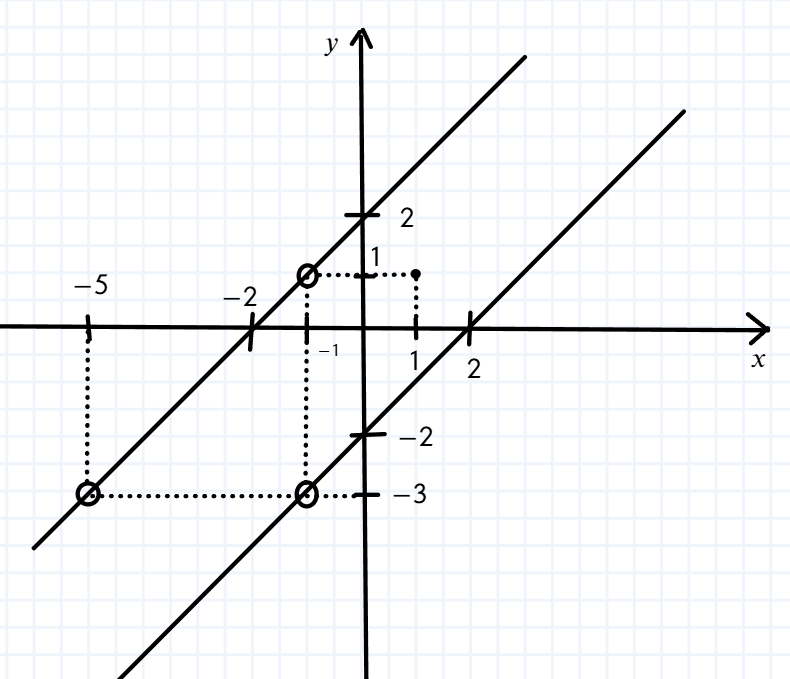
\includegraphics[scale=0.35]{gr7-97.png}}
\end{figure}\\
95. $\cfrac{(4-x(2y+x)-y^2)}{(2x-2y+xy-4)(x^2+y^2-2(x+y-1))}=0\Leftrightarrow$\\$
\begin{cases}

4-x(2y+x)-y^2=0,\\
(2x-2y+xy-4)(x^2+y^2-2(x+y-1))\neq0.
\end{cases}\Leftrightarrow$\\$
\begin{cases}
4-2xy-x^2-y^2=0,\\
x^2+y^2-2x-2y+2\neq0,\\
x(y+2)-2(y+2)\neq0.
\end{cases}\Leftrightarrow
\begin{cases}
4=(y+x)^2,\\
(x-1)^2+(y-1)^2\neq0,\\
(x-2)(y+2)\neq0.
\end{cases}\Leftrightarrow
\begin{cases}
\left[\begin{array}{l}
y=2-x,\\
y=-2-x,
\end{array}\right.\\
(x;y)\neq (1;1),\\
x\neq2,\\
y\neq-2.
\end{cases}$
\begin{figure}[ht!]
\center{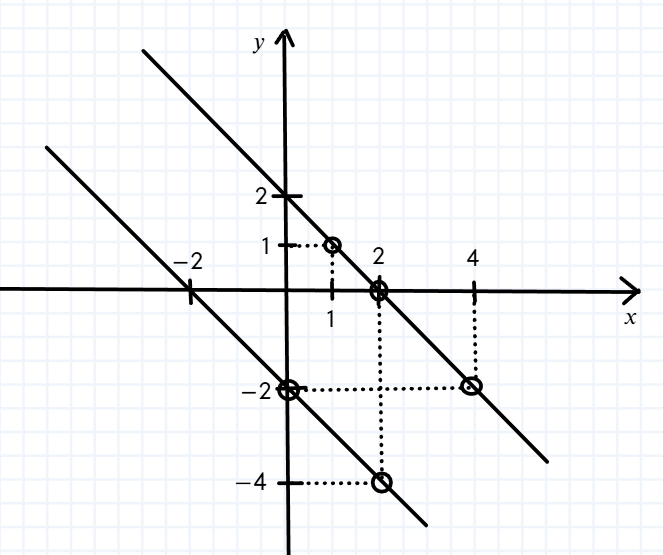
\includegraphics[scale=0.35]{gr7-98.png}}
\end{figure}
\newpage
\section{стандартные задачи решения}
1. Пусть картофеля привезли $x$т, а моркови --- $y.$ Тогда составим систему уравнений: \\$\begin{cases}0,4x+\cfrac{2}{3}y=20,\\ \cfrac{2}{3}\cdot0,6x+\cfrac{1}{3}y=15.\end{cases}\Leftrightarrow
\begin{cases}0,4x+\cfrac{2}{3}y=20,\\ 0,4x+\cfrac{1}{3}y=15.\end{cases}\Leftrightarrow
\begin{cases}\cfrac{1}{3}y=5,\\ 0,4x+\cfrac{1}{3}y=15.\end{cases}\Leftrightarrow
\begin{cases}y=15\text{ т},\\ x=25\text{ т}.\end{cases}$\\
2. Пусть арбузов привезли $x$т, а дынь --- $y.$ Тогда составим систему уравнений: \\$\begin{cases}\cfrac{1}{3}x+0,6y=44,\\ 0,75\cdot\cfrac{2}{3}x+0,4y=46.\end{cases}\Leftrightarrow
\begin{cases}\cfrac{1}{3}x+0,6y=44,\\ \cfrac{1}{2}x+0,4y=46.\end{cases}\Leftrightarrow
\begin{cases}x+1,8y=132,\\ x+0,8y=92.\end{cases}\Leftrightarrow
\begin{cases}y=40,\\ 0,4x+\cfrac{1}{3}y=15.\end{cases}\Leftrightarrow
\begin{cases}y=40\text{ т},\\ x=60\text{ т}.\end{cases}$\\
3. Пусть велосипедист предполагал ехать со скоростью $x$км/ч. Тогда она собирался потратить $\cfrac{210}{x}$ч, а потратил $\cfrac{105}{0,6x}+\cfrac{105}{1,4x}.$ Раз он опоздал на 2 часа, верно соотношение $\cfrac{210}{x}+2=\cfrac{105}{0,6x}+\cfrac{105}{1,4x},\ \cfrac{210}{x}+2=\cfrac{175}{x}+\cfrac{75}{x},\ \cfrac{40}{x}=2,\ x=20$км/ч.\\
4. Пусть участник авторалли предполагал ехать со скоростью $x$км/ч. Тогда она собирался потратить $\cfrac{360}{x}$ч, а потратил $\cfrac{180}{0,8x}+\cfrac{180}{1,2x}.$ Раз он затратил на 15 минут больше, верно соотношение $\cfrac{360}{x}+\cfrac{1}{4}=\cfrac{180}{0,8x}+\cfrac{180}{1,2x},\ \cfrac{360}{x}+\cfrac{1}{4}=\cfrac{225}{x}+\cfrac{150}{x},\ \cfrac{15}{x}=\cfrac{1}{4},\ x=60$км/ч.\\
5. Пусть скорость Вадика равна $x$км/ч, тогда скорость Любы $x+12$км/ч и верно соотношение $3(x+12)=5x,\ 3x+36=5x,\ 2x=36,\ x=18\text{ км/ч},\ x+12=30$км/ч.\\
6. Пусть скорость <<Жигулей>> равна $x$км/ч, тогда скорость BMW $1,5x$км/ч и верно соотношение $2x=1,5x+50,\ 0,5x=50,\ x=100\text{ км/ч},\ 1,5x=150$км/ч.\\
7. Пусть скорость машины на пути из A в B равна $x$км/ч, тогда скорость на обратном пути равна $x-10$км/ч и верно соотношение $1\cfrac{1}{4}x=1\cfrac{1}{2}(x-10),\
\cfrac{5}{4}x=\cfrac{3}{2}x-\cfrac{3}{2}\cdot10,\ \cfrac{1}{4}x=15,\ x=60$км/ч.\\
8. Пусть скорость теплохода в стоячей воде равна $x$км/ч, тогда верно соотношение $4\cfrac{1}{2}(x+2,4)=6\cfrac{3}{10}(x-2,4),\ 4,5x+10,8=6,3x-15,12,\
1,8x=25,92=14,4$км/ч.\\
9. За час автобус успеет отъехать от города на 60 км. Раз мотоциклист догнал его за $4-1=3$ часа, он догонял автобус со скоростью $60:3=20$км/ч, поэтому его скорость была равна $60+20=80$км/ч.\\
10. Через час после выезда расстояние между автобусом и пунктом B будет равно $300-60=240$км. Раз они с мотоциклистом встретились через 1,5 часа, скорость их сближения была равна $240:1,5=160$км/ч, значит скорость мотоциклиста равна $160-60=100$км/ч.\\
11. Первый поезд ехал $700:50=14$ч, а второй --- $(1231-700):59=9$ч, то есть первый выехал на $14-9=5$ часов раньше.\\
12. Первый автомобиль ехал $640:80=8$ч, а второй --- $(910-640):90=3$ч, то есть первый выехал на $8-3=5$ часов раньше.\\
13. Пусть расстояние от дома до стадиона равно $x$км, тогда так как пешком болельщик тратит на 1ч$+$30мин$=\cfrac{3}{2}$ч больше на дорогу, чем при поездке на велосипеде, верно соотношение $\cfrac{x}{5}=\cfrac{x}{10}+\cfrac{3}{2},\ \cfrac{x}{10}=\cfrac{3}{2},\ x=15$км.\\
14. Пусть расстояние от лагеря до станции равно $x$км, тогда так на велосипеде турист тратит на 30мин$+2$ч$=\cfrac{5}{2}$ч больше на дорогу, чем при поездке на мопеде, верно соотношение $\cfrac{x}{15}=\cfrac{x}{40}+\cfrac{5}{2},\ \cfrac{x}{24}=\cfrac{5}{2},\ x=60$км.\\
15. Пусть скорость катера в стоячей воде равна $x$км/ч, а скорость течения равна $y$км/ч, тогда верны равенства $\begin{cases} x+y=45,2,\\ x-y=36,2.\end{cases}
\Rightarrow 2y=9,\ y=4,5$км/ч.\\
16. Пусть скорость катера в стоячей воде равна $x$км/ч, а скорость течения равна $y$км/ч, тогда верны равенства $\begin{cases} x+y=40,6,\\ x-y=32,6.\end{cases}
\Rightarrow 2y=8,\ y=4$км/ч.\\
17. Пусть весь путь мотоциклиста равен $2x,$ тогда верно равенство $\cfrac{x}{45}+\cfrac{1}{6}+\cfrac{x}{60}=\cfrac{2x}{45},\
\cfrac{x+10}{60}=\cfrac{x}{45},\ 45x+450=60x,\ 15x=450,\ x=30,\ 2x=60$км.\\
18. Пусть весь путь автобуса равен $6x,$ тогда верно равенство $\cfrac{5x}{50}+\cfrac{1}{20}+\cfrac{x}{60}=\cfrac{6x}{50},\
\cfrac{x+3}{60}=\cfrac{x}{50},\ 50x+150=60x,\ 10x=150,\ x=15,\ 6x=90$км.\\
19. Пусть изначальная скорость автомобилиста была равна $x$км/ч, тогда верно соотношение $1\cfrac{1}{5}x=1\cfrac{3}{5}(x-20),\ \cfrac{6}{5}x=\cfrac{8}{5}x-32,\
\cfrac{2}{5}x=32,\ x=80$км/ч. Тогда расстояние между городом и посёлком равно $\cfrac{6}{5}\cdot80=96$км.\\
20. Пусть изначальная скорость автомобилиста была равна $x$км/ч, тогда верно соотношение $1\cfrac{4}{5}x=1\cfrac{2}{5}(x+20),\ \cfrac{9}{5}x=\cfrac{7}{5}x+28,\
\cfrac{2}{5}x=28,\ x=70$км/ч. Тогда расстояние между городом и посёлком равно $\cfrac{9}{5}\cdot70=126$км.\\
21. Скорость наполнения бассейна второй трубой равна $\cfrac{1}{10}-\cfrac{1}{35}=\cfrac{1}{14}$б/мин, значит она наполняет бассейн за 14 минут.\\
22. Скорость поедания торта Петей равна $\cfrac{1}{12}-\cfrac{1}{28}=\cfrac{1}{21}$т/мин, значит Петя съедает торт за 21 минуту.\\
23. Пусть скорость катера в стоячей воде равна $x$км/ч, тогда верно соотношение $3\cdot0,95x+40=3\cfrac{2}{3}\cdot1,05x,\
2,85x+40=3,85x,\ x=40,\ 0,95\cdot40=38$км/ч.\\
24. Пусть скорость лодки в стоячей воде равна $x$км/ч, тогда верно соотношение $3\cfrac{1}{3}\cdot0,9x+28=4\cdot1,1x,\
3x+28=4,4x,\ 1,4x=28,\ x=20,\ 1,1\cdot20=22$км/ч.\\
25. Пусть было задано выучить $x$ глаголов и $y$ существительных, тогда верны равенства\\
$\begin{cases}\cfrac{1}{12}x+\cfrac{1}{16}y=5,\\ \cfrac{1}{4}\cdot\cfrac{11}{12}x-\cfrac{1}{5}\cdot\cfrac{15}{16}y=8.\end{cases}\Leftrightarrow
\begin{cases}\cfrac{1}{4}x+\cfrac{3}{16}y=15,\\ \cfrac{11}{48}x-\cfrac{3}{16}y=8.\end{cases}\Leftrightarrow
\begin{cases}\cfrac{23}{48}x=23,\\ \cfrac{11}{48}x-\cfrac{3}{16}y=8.\end{cases}\Leftrightarrow
\begin{cases} x=48,\\ y=16.\end{cases}$\\
26. Пусть было задано решить $x$ задач по алгебре и $y$ по геометрии, тогда верны равенства\\
$\begin{cases}\cfrac{1}{15}x+\cfrac{1}{25}y=5,\\ \cfrac{1}{7}\cdot\cfrac{14}{15}x-\cfrac{1}{6}\cdot\cfrac{24}{25}y=-2.\end{cases}\Leftrightarrow
\begin{cases}\cfrac{4}{15}x+\cfrac{4}{25}y=20,\\ \cfrac{2}{15}x-\cfrac{4}{25}y=-2.\end{cases}\Leftrightarrow
\begin{cases}\cfrac{6}{15}x=18,\\ \cfrac{2}{15}x-\cfrac{4}{25}y=-2.\end{cases}\Leftrightarrow
\begin{cases} x=45,\\ y=50.\end{cases}$\\
27. Пусть зайцы едят со скоростью $x,$ а кролики $y$ тарелок моркови в секунду. Тогда верны равенства\\
$\begin{cases}2x+5y=\cfrac{1}{8},\\ 7x+4y=\cfrac{1}{4}.\end{cases}\Leftrightarrow
\begin{cases}8x+20y=\cfrac{1}{2},\\ 35x+20y=\cfrac{5}{4}.\end{cases}\Leftrightarrow
\begin{cases}8x+20y=\cfrac{1}{2},\\ 27x=\cfrac{3}{4}.\end{cases}\Leftrightarrow
\begin{cases} y=\cfrac{1}{72},\\ x=\cfrac{1}{36}.\end{cases}$
Тогда 1 заяц и 2 кролика едят со скоростью $\cfrac{1}{36}+2\cdot\cfrac{1}{72}=\cfrac{1}{18}$ тарелок в секунду и съедят одну тарелку моркови за 18 секунд.\\
28. Пусть зайцы едят со скоростью $x,$ а кролики $y$ тарелок в секунду. Тогда верны равенства\\
$\begin{cases}3x+2y=\cfrac{1}{12},\\ 5x+8y=\cfrac{1}{4}.\end{cases}\Leftrightarrow
\begin{cases}12x+8y=\cfrac{1}{3},\\ 5x+8y=\cfrac{1}{4}.\end{cases}\Leftrightarrow
\begin{cases}7x=\cfrac{1}{12},\\ 5x+8y=\cfrac{1}{4}.\end{cases}\Leftrightarrow
\begin{cases} x=\cfrac{1}{84},\\ y=\cfrac{1}{42}.\end{cases}$
Тогда 2 зайца и 1 кролик едят со скоростью $2\cdot\cfrac{1}{84}+\cfrac{1}{42}=\cfrac{1}{21}$ тарелок в секунду и съедят одну тарелку за 21 секунду.\\
29. На дорогу в одну сторону пешком Вася тратит $2,5:2=1,25$ч, значит на дорогу в одну сторону на трамвае он тратит $1,5-1,25=0,25$ч. Поэтому на дорогу в обе стороны на трамвае он потратит $2\cdot0,25=0,5$ч$=30$мин.\\
30. Пусть изначальная скорость пешехода равна $x$км/ч, тогда верно равенство $2,5x=2x+1\cdot(x-4),\ 0,5x=4,\ x=8$км/ч. Поэтому весь путь равен $2,5\cdot8=20$км.\\
31. Пусть карандаш стоит $x$ рублей, тогда ручка стоит $x+2$ рубля и верно равенство $27x+33(x+2)=246,\ 27x+33x+66=246,\ 60x=180,\ x=3$рубля.\\
32. Пусть скорость пешехода равна $x$м/мин, тогда скорость автобусов равна $6x$м/мин. Интервал, с которым автобусы проезжают мимо пешехода --- это то время, которое необходимо следующему автобусу, чтобы догнать пешехода в тот момент, когда он поравнялся с некоторым автобусом. Так как автобус догоняет пешехода за 12 минут, а догоняет его со скоростью $6x-x=5x$м/мин, расстояние между автобусами равно $5x\cdot12=60x$м. Интервал, за который автобусы проезжают мимо неподвижной остановки --- это как раз то время, которое необходимо автобусу на преодоление этого расстояния, то есть $60x:6x=10$минут.\\
33. Пусть скорость грузовика равна $x$км/ч, тогда верно равенство $10x=8(x+10),\ 10x=8x+80,\ 2x=80,\ x=40$км/ч, а расстояние $10\cdot40=400$км.\\
34. Пусть скорость второго поезда равна $x$км/ч, тогда скорость первого поезда равна $x+14$ и $(x+x+14)\cdot2\cfrac{2}{5}=600-240,\ \cfrac{24}{5}x+\cfrac{168}{5}=360,\ 24x+168=1800,\ 24x=1632,\ x=68$км/ч, $x+14=82$км/ч.\\
35. Пусть весь путь равен $2x$км, тогда верно равенство $\cfrac{x}{3}+\cfrac{x}{5}=8,\ 5x+3x=120,\ 8x=120,\ x=15,\ 2x=30$км.\\
36. Скорость Оксаны $\cfrac{1}{7}$ работы в час, Марины $\cfrac{1}{6},$ а Бориса Викторовича --- $\cfrac{1}{3}.$ Тогда всю работу они сделают за $\cfrac{\cfrac{1}{2}}{\cfrac{1}{7}}+\cfrac{\cfrac{1}{2}}{\cfrac{1}{7}+\cfrac{1}{6}+\cfrac{1}{3}}=\cfrac{7}{2}+\cfrac{7}{9}=4\cfrac{5}{18}$ч$=4$ч 16мин 40с. Марина выполнила $\cfrac{7}{9}\cdot\cfrac{1}{6}=\cfrac{7}{54}$ частей работы.\\
37. Пусть скорость автомобиля равна $x$км/ч, тогда верно равенство $2,5x+15=2(x+20),\ 2,5x+15=2x+40,\ 0,5x=25,\ x=50$км/ч. Тогда расстояние от города до посёлка равно $2,5\cdot50=125$км.\\
38. Пусть первый велосипедист потратил $2x$ч времени, тогда расстояние равно $25x+20x=45x.$ Второй велосипедист потратит на этот же путь $\cfrac{22,5x}{20}+
\cfrac{22,5x}{25}=2,025x>2x.$ Значит, первый велосипедист приедет раньше.\\
39. Пусть скорости работы девочек равны $t,\ l$ и $k$ соответственно. Тогда верны равенства\\ $\begin{cases}t+l=\cfrac{1}{12},\\ t+k=\cfrac{1}{20},\\ l+k=\cfrac{1}{15}.\end{cases}$ Отсюда $t+l+k=\cfrac{\cfrac{1}{12}+\cfrac{1}{20}+\cfrac{1}{15}}{2}=\cfrac{1}{10},$ поэтому $t=\cfrac{1}{10}-\cfrac{1}{15}=\cfrac{1}{30},\ k=\cfrac{1}{10}-\cfrac{1}{12}=\cfrac{1}{60},\ l=\cfrac{1}{10}-\cfrac{1}{20}=\cfrac{1}{20}.$ Значит, их зарплаты должны соотноситься как $\cfrac{1}{30}:\cfrac{1}{60}:\cfrac{1}{20}=2:1:3.$ Поэтому Таня должна получить $\cfrac{2}{6}\cdot1800=600$р, Катя $\cfrac{1}{6}\cdot1800=300$р и Люба $\cfrac{3}{6}\cdot1800=900$р.\\
40. Пусть скорость мотоцикла равна $x$км/ч, тогда скорость автомобиля равна $x+30$км/ч. За время, прошедшее до встречи, вместе они проедут два расстояния от станции до посёлка, значит $(x+x+30)\cdot1\cfrac{3}{5}=2\cdot104,\ \cfrac{16}{5}x+48=208,\ \cfrac{16}{5}x=160,\ x=50$км/ч. Значит, встреча произошла на расстоянии $50\cdot\cfrac{8}{5}=80$км от станции. \\
41. За 2 часа первая труба заполнит бассейн на $\cfrac{1}{12}\cdot2=\cfrac{1}{6}$ часть. Значит, на то, чтобы заполнить остаток бассейна до конца, уйдёт $\cfrac{\cfrac{5}{6}}{\cfrac{1}{12}+\cfrac{1}{20}}=6\cfrac{1}{4}$ч, поэтому всего бассейн был заполнен за $2+6\cfrac{1}{4}=8\cfrac{1}{4}$ч или 8 ч 15 мин. Первая труба работала всё время, значит она заполнила $\cfrac{1}{12}\cdot\cfrac{33}{4}=\cfrac{11}{16}$ бассейна.\\
42. Наташа успеет пройти $5\cdot\cfrac{1}{30}=\cfrac{1}{6}$ расстояния до школы, значит Лена догонит её через $\cfrac{\cfrac{1}{6}}{\cfrac{1}{20}-\cfrac{1}{30}}=10$минут.\\
43. Пусть ширина комнаты равна $x$м, тогда длина равна $x+1$м и площадь $x(x+1)=x^2+x\text{м}^2.$ Площадь ковра, закрывающего только часть комнаты, равна $(x-0,5)(x+0,5)=x^2-0,25,$ что меньше на $x^2+x-(x^2-0,25)=x+0,25\text{м}^2.$ Исходя из стоимости ковра, найдём эту площадь: $x+0,25=\cfrac{2550}{600}=4,25\Rightarrow x=4$м, $x+1=5$м.\\
44. Пусть собственная скорость катера равна $x$км/ч, а скорость течения --- $y$км/ч. Тогда получаем систему уравнений: $\begin{cases}3(x+y)+5(x-y)=76,\\
6(x+y)=9(x-y).\end{cases}\Leftrightarrow\begin{cases}8x-2y=76,\\
15y=3x.\end{cases}\Leftrightarrow\begin{cases}40y-2y=76,\\
5y=x.\end{cases}\Leftrightarrow\begin{cases}38y=76,\\
5y=x.\end{cases}\Leftrightarrow\begin{cases} y=2\text{км/ч},\\
x=10\text{км/ч}.\end{cases}$\\
45. Петя придёт домой через $2,8:4=0,7$ч. За это время Серёжа проедет $42\cdot0,7=29,4$км, что составляет $29,4:2,8=10,5$ расстояний от дома до школы. Значит, он встретит Петю 11 раз (он встречает его каждый раз, когда проезжает полное расстояние, и встретит 11-ый раз, когда будет проезжать последнюю половину расстояния по направлению от дома к школе).\\
46. В метро Эрвин едет $8:\cfrac{2}{9}=36$мин, тогда пешком он идёт $36-29=7$мин, на троллейбусе едет $36:2=18$мин. Таким образом, всего он тратит $36+7+18+8=69$минут или 1 час 9 минут.\\
47. В метро Эрвин едет $9:\cfrac{3}{13}=39$мин, тогда пешком он идёт $39-31=8$мин, на троллейбусе едет $39:3=13$мин. Таким образом, всего он тратит $39+8+13+9=69$минут или 1 час 9 минут.\\
48. Один садовник за один час посадит $30:5:3=2$ дерева, значит 4 садовника за 4 часа посадят $2\cdot4\cdot4=32$ дерева.\\
49. Им потребуется $\cfrac{1}{\cfrac{1}{6}+\cfrac{1}{12}}=4$дня.\\
50. Пусть бригады пашут со скоростями $x,\ y$ и $z$ гектаров в день соответственно, а первое поле имеет площадь $S$ гектаров. Тогда имеем систему уравнений
$\begin{cases}3(x+y+z)=S,\\ 6(y+z)=96-S,\\ x+y+z+8x=96-S.\end{cases}\Leftrightarrow
\begin{cases}3x+3y+3z+6y+6z=96,\\ 6y+6z=96-S,\\ 9x+y+z=96-S.\end{cases}\Leftrightarrow
\begin{cases}3x+9y+9z=96,\\ 6y+6z=9x+y+z,\\ 9x+y+z=96-S.\end{cases}\Leftrightarrow
\begin{cases}x+3(y+z)=32,\\ 9x=5(y+z),\\ 9x+y+z=96-S.\end{cases}\Rightarrow$\\$
x+3\cdot\cfrac{9x}{5}=32,\ 32x=180,\ x=5$га/д.\\
51. Пусть скорости первого и второго поездов равны $x$ и $y$км/ч соответственно, расстояние между B и C равно $S,$ а затрачиваемое до встречи время равно $t.$ Тогда имеем систему уравнений
$\begin{cases} tx=60+S,\\ ty=S,\\ (t-2)(x+25)=60+S,\\ (t-2)(y+20)=S\end{cases}$. Поделив первое уравнение на второе, а третье на четвёртое, получим соотношение $\cfrac{x}{y}=\cfrac{60+S}{S}=\cfrac{x+25}{y+20},$ откуда $xy+20x=xy+25y,\ 20x=25y,\ x=1,25y.$ Поэтому $\cfrac{60+S}{S}=1,25,\ 60+S=1,25S,\ 0,25S=60,\ S=240$км. Перепишем первое и третье уравнения: $\begin{cases}tx=300,\\(t-2)(x+25)=300\end{cases}\Leftrightarrow\begin{cases}tx=300,\\tx+25t-2x-50=300\end{cases}\Leftrightarrow
\begin{cases}tx=300,\\25t=2x+50\end{cases}\Rightarrow$\\$ x\cdot\cfrac{2x+50}{25}=300,\ 2x^2+50x=7500,\ 4x^2+100x=15000,\ 4x^2+100x+625=15625,\ (2x+25)^2=125^2,\ x=50$км/ч, тогда $y=50:1,25=40$км/ч.\\
52. Они съедят банку за $\cfrac{1}{\cfrac{1}{10}+\cfrac{1}{12}+\cfrac{1}{15}}=4$минуты.\\
53. Вася вскапывает грядку за $\cfrac{1}{\cfrac{1}{10}-\cfrac{1}{15}}=30$ минут, что на $30-15=15$ минут дольше, чем Петя.\\
54. Пусть скорость первого пешехода равна $x$м/мин, а второго --- $y$м/мин. Тогда расстояние от места встречи до пункта B равно $50x,$ а расстояние от места встречи до пункта A равно $18y.$ До места встречи пешеходы добрались одновременно, значит $\cfrac{50x}{y}=\cfrac{18y}{x},\ 50x^2=18y^2,\ 25x^2=18y^2,\ 5x=3y\Rightarrow50x=30y$ и до места встречи пешеходы шли $30y:y=30$ минут.\\
55. Пусть скорость первого пешехода равна $x$м/мин, а второго --- $y$м/мин. Тогда расстояние от места встречи до пункта B равно $45x,$ а расстояние от места встречи до пункта A равно $20y.$ До места встречи пешеходы добрались одновременно, значит $\cfrac{45x}{y}=\cfrac{20y}{x},\ 45x^2=20y^2,\ 9x^2=4y^2,\ 3x=2y\Rightarrow45x=30y$ и до места встречи пешеходы шли $30y:y=30$ минут.\\
56. Пусть мастер работает со скоростью $x$ плана в час, а ученик --- $y.$ Тогда имеем систему уравнений
$\begin{cases}2x+3y=0,9,\\ 3x+2y=1,15.\end{cases}\Leftrightarrow
\begin{cases}6x+9y=2,7,\\ 6x+4y=2,3.\end{cases}\Rightarrow 5y=0,4,\ y=0,08.$ Таким образом, ученику на выполнение плана понадобится $1:0,08=12,5$ часов.\\
57. Пусть мастер работает со скоростью $x$ плана в час, а ученик --- $y.$ Тогда имеем систему уравнений
$\begin{cases}2x+3y=\cfrac{4}{5},\\ 3x+2y=1,05.\end{cases}\Leftrightarrow
\begin{cases}6x+9y=2,4,\\ 6x+4y=2,1.\end{cases}\Rightarrow 5y=0,3,\ y=0,06.$ Таким образом, ученику на выполнение плана понадобится $1:0,06=16\cfrac{2}{3}$ часов или 16 часов 40 минут.\\
58. Средняя скорость $V$ равна $\cfrac{60+30}{\cfrac{60}{40}+\cfrac{30}{60}}=45.$\\
59. Составим уравнение нахождения средней скорости: $50=\cfrac{80+20}{\cfrac{80}{60}+\cfrac{20}{V}}=\cfrac{75V}{V+15},\ 50V+750=75V,\ 25V=750,\ V=30.$\\
60. Средняя скорость $V$ равна $\cfrac{80+24}{\cfrac{80}{60}+\cfrac{24}{34}}=51.$\\
61. Составим уравнение нахождения средней скорости: $72=\cfrac{100+50}{\cfrac{100}{80}+\cfrac{50}{V}}=\cfrac{120V}{V+40},\ 72V+2880=120V,\ 48V=2880,\ V=60.$\\
62. Пусть масса первоначального сплава в граммах равна $x.$ Тогда золота в нём $0,3x$ и $0,3x-2=0,25(x-2+12),\ 0,3x-2=0,25x+2,5,\ 0,05x=4,5,\ x=90$г.\\
63. Пусть процентное содержание меди в первоначальном сплаве в процентах равно $x.$ Тогда меди в этом сплаве $\cfrac{40x}{100}$ и $\cfrac{40x}{100}+5=\cfrac{x+10}{100}\cdot45,\ 40x+500=45x+450,\ 5x=50,\ x=10\%,$ а олова --- $100-10=90\%.$\\
64. Пусть масса первоначального сплава в граммах равна $x.$ Тогда серебра в нём $0,7x$ и $0,7x-4=0,5(x-4+10),\ 0,7x-4=0,5x+3,\ 0,2x=7,\ x=35$г.\\
65. Пусть процентное содержание меди в первоначальном сплаве в процентах равно $x.$ Тогда меди в этом сплаве $\cfrac{60x}{100}$ и $\cfrac{60x}{100}=\cfrac{x-10}{100}\cdot72,\ 60x=72x-720,\ 12x=720,\ x=60\%.$\\
66. Поезд проехал 1 час 40 минут, то есть $\cfrac{5}{3}$ч с первоначальной скоростью и 1 час со сниженной скоростью (так как опоздал на 10 минут). Пусть первоначальная скорость поезда равна $x$км/ч, тогда расстояние между двумя пунктами равно $2,5x$ с одной стороны и  $\cfrac{5}{3}x+x-10=\cfrac{8}{3}x-10$ с другой, поэтому $2,5x=\cfrac{8}{3}x-10,\ \cfrac{1}{6}x=10,\ x=60$км/ч.\\
67. Пусть один автомобиль проехал $x$км, тогда другой проехал $x+60$ и $x+x+60=840,\ 2x=780,\ x=390$км. Значит, один автомобиль проехал 390 км, а другой --- $840-390=450$км. Так как $\cfrac{390}{60}<\cfrac{450}{65},$ 390 км должен был проехать второй автомобиль, а 450 км --- первый (так как первый ехал дольше). Тогда первый ехал $\cfrac{450}{60}=7,5$ч, а второй --- $\cfrac{390}{65}=6$ч, поэтому он выехал позже на $7,5-6=1,5$ часа.\\
68. Поезд проехал 1,5 ч с первоначальной скоростью и $2+\cfrac{8}{60}=\cfrac{32}{15}$ часа со сниженной скоростью (так как опоздал на 8 минут). Пусть первоначальная скорость поезда равна $x$км/ч, тогда расстояние между двумя пунктами равно $3,5x$ с одной стороны и  $1,5x+\cfrac{32}{15}(x-5)=\cfrac{109}{30}x-\cfrac{32}{3}$ с другой, поэтому $3,5x=\cfrac{109}{30}x-\cfrac{32}{3},\ \cfrac{2}{15}x=\cfrac{32}{3},\ x=80$км/ч.\\
69. Пусть один автомобиль проехал $x$км, тогда другой проехал $x+40$ и $x+x+40=680,\ 2x=640,\ x=320$км. Значит, один автомобиль проехал 320 км, а другой --- $680-320=360$км. Если первый ехал $\cfrac{360}{80}=4,5$ч, а второй --- $\cfrac{320}{100}=3,2$ч, то второй выехал позже на $4,5-3,2=1,3$ часа. Если первый ехал $\cfrac{320}{80}=4$ч, а второй --- $\cfrac{360}{100}=3,6$ч, то второй выехал позже на $4-3,6=0,4$ часа. Возможны оба случая.\\
70. Скорость движения лодки по течению реки равна $9+1=10$км/ч, а против течения --- $9-1=8$км/ч. Пусть она отплыла на $x$ километров, тогда должно выполняться неравенство $\cfrac{x}{10}+\cfrac{x}{8}\leqslant9,\ \cfrac{9x}{40}\leqslant9,\ x\leqslant40$км. Значит, максимум лодка может отплыть на 40 километров.\\
71. Скорость движения лодки по течению реки равна $8+2=10$км/ч, а против течения --- $8-2=6$км/ч. Пусть она отплыла на $x$ километров, тогда должно выполняться неравенство $\cfrac{x}{10}+\cfrac{x}{6}\leqslant4,\ \cfrac{8x}{30}\leqslant4,\ x\leqslant15$км. Значит, максимум лодка может отплыть на 15 километров.\\
72. Пусть скорости покраски мальчиков равны $x,\ y$ и $z$ (забора в час). Тогда имеет место система $\begin{cases} x+y=\cfrac{1}{4},\\ y+z=\cfrac{1}{12},\\ x+z=\cfrac{1}{9}.\end{cases}\Rightarrow x+y+z=\cfrac{1}{2}\cdot\left(\cfrac{1}{4}+\cfrac{1}{12}+\cfrac{1}{9}\right)=\cfrac{2}{9}.$ Значит, втроём мальчики покрасят забор за $1:\cfrac{2}{9}=4,5$ часа.\\
73. Пусть скорости обработки грядки девочек равны $x,\ y$ и $z$ (грядки в час). Тогда имеет место система $\begin{cases} x+y=\cfrac{1}{9},\\ y+z=\cfrac{1}{4},\\ x+z=\cfrac{1}{12}.\end{cases}\Rightarrow x+y+z=\cfrac{1}{2}\cdot\left(\cfrac{1}{9}+\cfrac{1}{4}+\cfrac{1}{12}\right)=\cfrac{2}{9}.$ Значит, втроём девочки обработают грядку за $1:\cfrac{2}{9}=4,5$ часа.\\
74. Пусть скорость набора рукописи куратором равна $x$ (рукописи в час), тогда у студенток она $\cfrac{x}{2}$ и $\cfrac{x}{3}$ и $\cfrac{x}{2}+\cfrac{x}{3}=\cfrac{1}{6},\ \cfrac{5x}{6}=\cfrac{1}{6},\ x=\cfrac{1}{5}.$ Значит, куратор наберёт рукопись за $1:\cfrac{1}{5}=5$ часов.\\
75. Расстояние они проехали одинаковое, значит один мотоциклист проезжал его со скоростью в три раза большей скорости другого. Пусть скорость поезда равна $x$ км/ч, тогда мотоциклист, едущий навстречу, проезжает мимо него со скоростью $x+100,$ а едущий в том же направлении --- со скоростью $100-x.$ Таким образом, $x+100=3(100-x),\ x+100=300-3x,\ 4x=200,\ x=50$км/ч.\\
76. Пусть расстояние от дома до школы равно $S$м, а скорость Пети равна $v$ м/с, тогда $3\cdot\cfrac{S}{v+3}=\cfrac{S}{v},$ откуда $3v=v+3,\ 2v=3,\ v=1,5$м/с. Значит, изначально время на путь от дома до школы занимал $\cfrac{S}{1,5}$с, а после увеличения скорости на 6 м/с будет занимать $\cfrac{S}{7,5}$с, что в $\cfrac{S}{1,5}:\cfrac{S}{7,5}=5$ раз меньше.\\
77. Машина сэкономила время на дорогу от места встречи до Васиного дома и обратно, получилось 10 минут. Значит, от места встречи до дома она ехала бы 5 минут, поэтому встретились она на 5 минут раньше назначенного времени, в 15:55. Значит, Вася прошёл расстояние от дома до места встречи за 55 минут, в 11 раз дольше, чем ехала бы машина. Поэтому скорость машины в 11 раз больше Васиной и равна $11\cdot6=66$ км/ч.\\
78. Пусть морковь занимает $x$ ящиков, тогда картофель занимает $2x$ ящиков, а капуста --- $(x+2x)\cdot3=9x$ ящиков. Тогда под хранение капусты отведено $\cfrac{9x}{x+2x+9x}\cdot100\%=75\%$ ящиков.\\
79. Пусть морковь занимает $x$ ящиков, тогда картофель занимает $3x$ ящиков, а капуста --- $(x+3x)\cdot9=36x$ ящиков. Тогда под хранение капусты отведено $\cfrac{36x}{x+3x+36x}\cdot100\%=90\%$ ящиков.\\
80. Пусть автомобиль проехал $x$км, тогда ему осталось проехать $x+20$км, и выполнено соотношение $\cfrac{x}{90}+\cfrac{x+20}{90\cdot1,2}=\cfrac{x+x+20}{100},\
\cfrac{x}{90}+\cfrac{x+20}{108}=\cfrac{x+10}{50}\Big|\cdot2700,\
30x+25(x+20)=54(x+10),\ 30x+25x+500=54x+540,\ x=40$км. Таким образом, весь путь составлял $40+40+20=100$км.\\
81. Пусть автомобиль увеличил скорость через $x$км от старта, тогда ему оставалось проехать ещё $200-x$км, и выполнено соотношение
$\cfrac{x}{135}+\cfrac{200-x}{135\cdot1,2}=\cfrac{200}{150},\
\cfrac{x}{135}+\cfrac{200-x}{162}=\cfrac{4}{3}\Big|\cdot 810,\
6x+5(200-x)=1080,\ 6x+1000-5x=1080,\ x=80$км.
\newpage
\section{нестандартные задачи решения}
1. а) Да, так как сумма его цифр равна $1998=3\cdot666.$ б) Нет, так как последняя цифра нечётна. в) Нет, так как оно не делится на 2.\\
2. а) Нет, так как сумма его цифр равна $2\cdot239,$ что не делится на 3. б) Да, так как последняя цифра чётна. в) Нет, так как оно не делится на 3.\\
3. Раз $\text{НОД}(a,b)=a,\ b$ делится на $a,$  а поэтому  $\text{НОК}(a,b)=b.$\\
4. Раз $\text{НОК}(a,b)=a,\ a$ делится на $b,$  а поэтому  $\text{НОД}(a,b)=b.$\\
5. Всего ходящих в кружки ребят $35-10=25.$ Если сложить математиков и членов кружка <<Умелые руки>>, получим $20+11=31,$ что на $31-25=6$ больше, чем общее количество ребят, посещающих кружки. Это произошло потому, что математиков, посещающих кружок <<Умелые руки>>, мы посчитали 2 раза, значит их и было 6.\\
6. Всего ходящих в кружки ребят $37-10=27.$ Если сложить физиков и биологов, получим $19+13=32,$ что на $32-27=5$ больше, чем общее количество ребят, посещающих кружки. Это произошло потому, что физиков, посещающих кружок биологии, мы посчитали 2 раза, значит их и было 5.\\
7. Обозначим первое число буквой $x,$ тогда $x(x+2)+120=(x+4)(x+6),\ x^2+2x+120=x^2+6x+4x+24,\ 8x=96,\ x=12.$ Значит, это числа 12, 14, 16, 18.\\
8. Обозначим первое число буквой $x,$ тогда $x(x+2)+144=(x+4)(x+6),\ x^2+2x+144=x^2+6x+4x+24,\ 8x=120,\ x=15.$ Значит, это числа 15, 17, 19, 21.\\
9. Если $a$ и $b$ имеют одинаковую чётность, то оба множителя чётны и произведение должно делиться на 4, а 6 не делится. Если
$a$ и $b$ имеют разную чётность, то оба множителя нечётны и произведение должно быть нечётно, а 6 чётно. Значит, таких чисел не существует.\\
10. Если $a$ и $b$ имеют одинаковую чётность, то оба множителя чётны и произведение должно делиться на 4, а 10 не делится. Если
$a$ и $b$ имеют разную чётность, то оба множителя нечётны и произведение должно быть нечётно, а 10 чётно. Значит, таких чисел не существует.\\
11. Пусть это было число $\overline{abc}=100a+10b+c,$ тогда $100a+10b+c-a-b-c=189,\ 99a+9b=189,\ 11a+b=21.$ Если $a=1,$ то $b=10,$ что невозможно, так как это цифра. Если $a\geqslant2,$ то $11a\geqslant22>21.$ Значит, такого числа не существует и 189 получиться не могло.\\
12. Пусть это было число $\overline{abc}=100a+10b+c,$ тогда $100a+10b+c-a-b-c=180,\ 99a+9b=180,\ 11a+b=20.$ Это возможно, если $a=1,\ b=9,$ при этом цифра $c$ может быть какой угодно. Например, $190-(1+9+0)=180.$\\
13. Введём систему координат с центром в левом нижнем угле прямоугольника. Тогда диагональ --- это прямая $y=\cfrac{239}{566}x.$ Она не проходит ни через один узел сетки внутри прямоугольника, так как в таком случае и $x,$ и $y$ были бы целыми числами что невозможно, так как $x<566$ и $\text{НОД}(239,566)=1,$ поэтому домножение на $x$ не сможет сократить полностью знаменатель. Значит, диагональ пересекает по 1 разу в разных точках все вертикальные прямые $x=1,\ 2,\ \ldots 566$ и горизонтальные прямые $y=1,\ 2,\ \ldots 239,$ за исключением последней точки, правой верхней вершины прямоугольника. Последняя точка считается два раза, поэтому всего точек пересечения $566+239-1=804.$ Каждой точке пересечения можно сопоставить ту клетку, в которой диагональ находилась перед пересечением (будем считать, что мы двигаемся вправо-вверх), тогда диагональ пересекает 804 клетки.
\begin{figure}[ht!]
\center{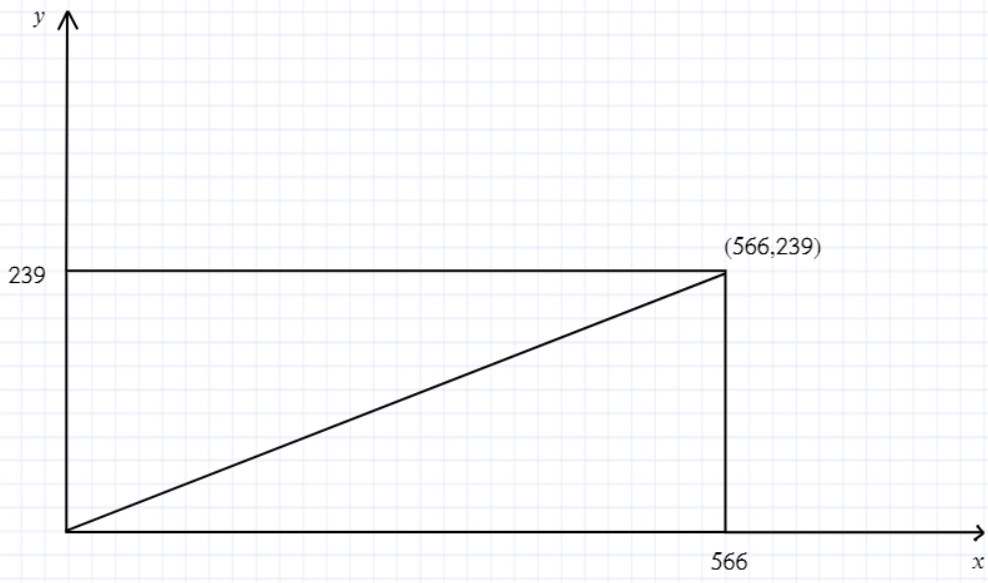
\includegraphics[scale=0.25]{566.png}}
\end{figure}\\
14. Введём систему координат с центром в левом нижнем угле прямоугольника. Тогда диагональ --- это прямая $y=\cfrac{239}{366}x.$ Она не проходит ни через один узел сетки внутри прямоугольника, так как в таком случае и $x,$ и $y$ были бы целыми числами что невозможно, так как $x<366$ и $\text{НОД}(239,366)=1,$ поэтому домножение на $x$ не сможет сократить полностью знаменатель. Значит, диагональ пересекает по 1 разу в разных точках все вертикальные прямые $x=1,\ 2,\ \ldots 366$ и горизонтальные прямые $y=1,\ 2,\ \ldots 239,$ за исключением последней точки, правой верхней вершины прямоугольника. Последняя точка считается два раза, поэтому всего точек пересечения $366+239-1=604.$ Каждой точке пересечения можно сопоставить ту клетку, в которой диагональ находилась перед пересечением (будем считать, что мы двигаемся вправо-вверх), тогда диагональ пересекает 604 клетки.
\begin{figure}[ht!]
\center{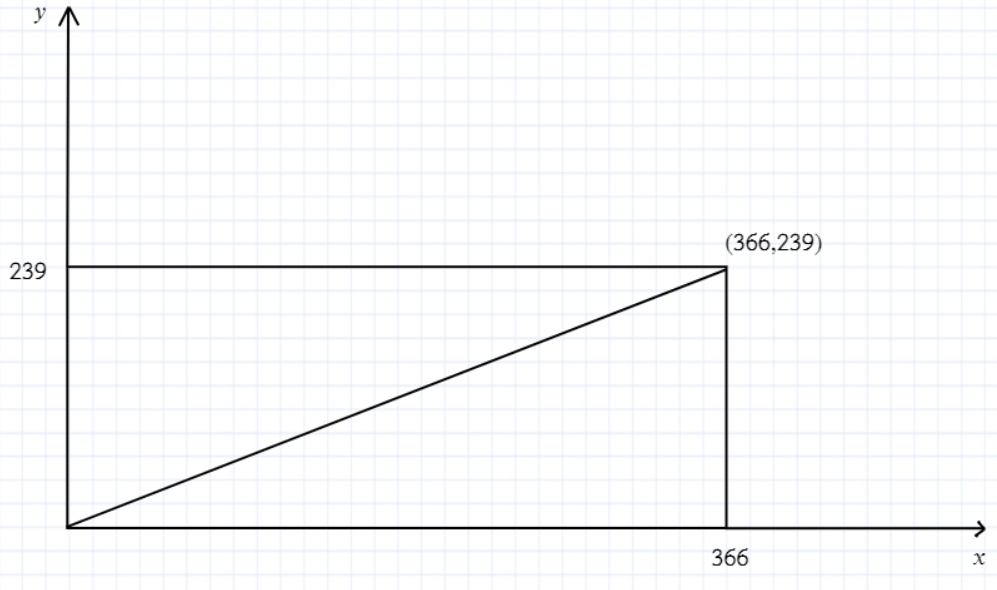
\includegraphics[scale=0.25]{5666.png}}
\end{figure}\\
15. Любые две окружности могут иметь максимум две точки пересечения. Количество способов выбрать две окружности из 9 равно $\cfrac{9\cdot8}{2}=36,$ тогда точек пересечения будет $36\cdot2=72.$\\
16. В этой последовательности на месте с номером $2k$ стоит число $k,$ а на месте с номером $2k+1$--- число $-k.$ Тогда на 366-м места стоит число $366:2=183,$ а число 366 стоит на месте $366\cdot2=732.$\\
17. В этой последовательности на месте с номером $2k$ стоит число $k,$ а на месте с номером $2k+1$--- число $-k.$ Тогда на 239-м места стоит число $-(239-1):2=-119,$ а число 239 стоит на месте $239\cdot2=478.$\\
18. Сложим числитель и знаменатель: $5k^2+7k+11+8k^2+6k+2=13k^2+13k+13=13(k^2+k+1).$ Так как сумма числителя и знаменателя делится на 13, знаменатель тоже делится на 13, а значит дробь можно сократить на 13.\\
19. Сложим числитель и знаменатель: $3k^2+7k+1+8k^2+4k+10=11k^2+11k+11=11(k^2+k+1).$ Так как сумма числителя и знаменателя делится на 11, знаменатель тоже делится на 11, а значит дробь можно сократить на 11.\\
20. Сумма возрастов игроков до удаления была равна $11\cdot22=242$ года, а после удаления стала равна $10\cdot21=210.$ Значит, удалённому игроку было $242-210=32$ года.\\
21. Сумма возрастов игроков до удаления была равна $11\cdot26=288$ лет, а после удаления стала равна $10\cdot25=250.$ Значит, удалённому игроку было $286-250=36$ лет.\\
22. Разложим число 1072 на простые множители: $1072=2^4\cdot67.$ Эти множители необходимо разбить на две группы так, чтобы произведение множителей в первой группе было больше 100 (цена книги), а во второй --- больше 6 (количество книг). Это можно сделать единственным образом: $1072=8\cdot134,$ значит книг было 8.\\
23. Разложим число 1071 на простые множители: $1071=3^2\cdot7\cdot17.$ Эти множители необходимо разбить на две группы так, чтобы произведение множителей в первой группе было больше 100 (цена книги), а во второй --- больше 5 (количество книг). Это можно сделать двумя способами: $1071=9\cdot119$ и $1071=7\cdot153.$ Значит, книг могло быть 7 или 9.\\
24. а) Пусть в первом штабеле $x$ коробок по 19кг. Тогда в нём $30-x$ коробок по 49 кг, во втором штабеле $33-x$ коробок по 19кг и $30-(33-x)=x-3$ коробки по 49 кг.
Поэтому $A=|S_1-S_2|=|19x+49(30-x)-19(33-x)-49(x-3)|=|990-60x|=30|33-2x|\geqslant30$кг, так как $|33-2x|\geqslant1.$\\
б) Пусть в первом штабеле $x$ коробок по 19кг и $y$ коробок по 49кг. Тогда во втором штабеле $33-x$ коробок по 19кг и $27-y$ коробок по 49кг. Поэтому
$A=|S_1-S_2|=|19x+49y-19(33-x)-49(27-y)|=2|19x+49y-975|.$ Если это выражение равно нулю, то $19x+49y=975,\ 19(x+y)=15(65-2y).$ Правая часть нечётна и делится на 15, числа 19 и 15 взаимно просты, значит $x+y$ может быть равно только 15 или 45 $(x+y\leqslant33+27=60<75).$ В первом случае $2y=65-19=46,\ y=23,\ x=15-23=-8,$ что невозможно. Во втором случае $2y=65-57=8,\ y=4,\ x=45-4=41>30,$ что также невозможно. Значит, $A$ не может быть равно нулю.\\
25. а) Пусть в первом штабеле $x$ коробок по 13кг. Тогда в нём $22-x$ коробок по 29 кг, во втором штабеле $25-x$ коробок по 13кг и $22-(25-x)=x-3$ коробки по 29 кг.
Поэтому $A=|S_1-S_2|=|13x+29(22-x)-13(25-x)-29(x-3)|=|400-32x|=16|25-2x|\geqslant16$кг, так как $|25-2x|\geqslant1.$\\
б) Пусть в первом штабеле $x$ коробок по 13кг и $y$ коробок по 29кг. Тогда во втором штабеле $25-x$ коробок по 13кг и $19-y$ коробок по 29кг. Поэтому
$A=|S_1-S_2|=|13x+29y-13(25-x)-29(19-y)|=2|13x+29y-438|.$ Если это выражение равно нулю, то $13x+29y=438,\ 13(x+y)=2(219-8y).$ Правая часть делится на 13, числа 2 и 13 взаимно просты, значит $219-8y$ делится на 13. Перебором остатков от деления на 13 найдём, что $y$ (при условии $0\leqslant y\leqslant19)$ может быть равно только 3 или 16. Тогда в первом случае $x=30-3=27>25,$ что невозможно. Во втором случае $x=14-16=-2,$ что также невозможно. Значит, $A$ не может быть равно нулю.\\
26. а) Да, подбором (отталкиваясь от числа 8) найдём подходящий пример.
\begin{figure}[ht!]
\center{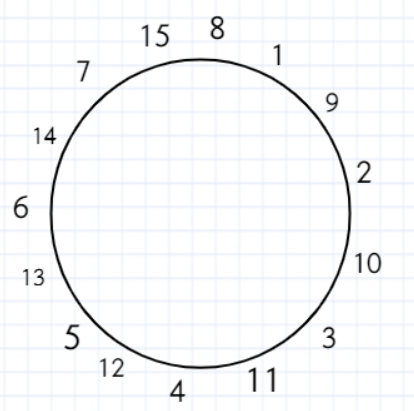
\includegraphics[scale=0.35]{krug1.png}}
\end{figure}\\
б) Нет, так как ни одно число не может стоять рядом с 8.\\
27. а) Да, подбором (отталкиваясь от числа 9) найдём подходящий пример.
\begin{figure}[ht!]
\center{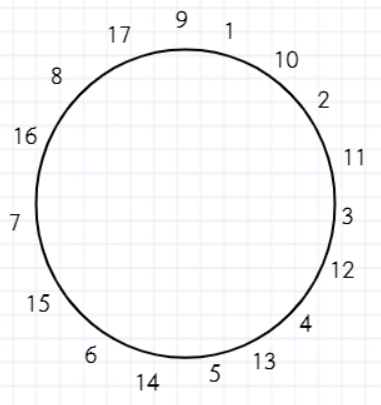
\includegraphics[scale=0.35]{krug2.png}}
\end{figure}\\
б) Нет, так как ни одно число не может стоять рядом с 9.\\
28. Число кратно трём тогда и только тогда, когда его сумма цифр делится на три. Если первые две цифры числа отличаются на 1, их сумма нечётна. Поэтому если последняя цифра числа равна 7, то сумма двух первых может быть равна 5, 11 или 17. Таких чисел 6: 237, 327, 567, 657, 897, 987. Если же последняя цифра числа равна 8, то сумма первых двух может быть равна 1, 7 или 13. Таких чисел 5: 108, 348, 438, 678, 768. Таким образом, всего {\it хороших} чисел $6+5=11.$\\
29. Число кратно трём тогда и только тогда, когда его сумма цифр делится на три. Если первые две цифры числа отличаются на 2, их сумма чётна. Поэтому если последняя цифра числа равна 6, то сумма двух первых может быть равна 6 или 12. Таких чисел 4: 246, 426, 576, 756. Если же последняя цифра числа равна 7, то сумма первых двух может быть равна 2, 8 или 14. Таких чисел 5: 207, 357, 537, 687, 867. Таким образом, всего {\it интересных} чисел $4+5=9.$\\
30. Посчитаем массу всех глыб: $50\cdot700+60\cdot1000+80\cdot1500=215000\text{ кг}=215\text{ т}.$ Будем сразу пытаться решить пункт б): $43\cdot5=215,$ значит если эти глыбы и можно погрузить на 43 грузовика, то пустого пространства ни в одном грузовике остаться не должно. Если пустого пространства не остаётся, глыб по 700кг в грузовике может быть только 5, тогда оставшиеся 1500кг занимает одна глыба по 1500кг. Понадобится $50:5=10$ грузовиков, на которые мы погрузим все глыбы по 700кг и 10 глыб по 1500кг. Остаётся ещё 60 глыб по 1000кг и $80-10=70$ глыб по 1500кг. Если пустого пространства не остаётся, глыб по 1500кг в грузовике может быть только 2, тогда оставшиеся 2000кг занимают две глыбы по 1000кг. Понадобится $60:2=30$ грузовиков, на которые мы погрузим все глыбы по 1000кг и $2\cdot30=60$ глыб по 1500кг. Таким образом, останется ещё $70-60=10$ глыб по 1500кг. Уже понятно, что в 43 грузовика все глыбы погрузить не получится, так как без пустого пространства погрузить оставшиеся глыбы невозможно. В 44 грузовика их можно погрузить следующим образом: в 3 грузовика поместить по 3 глыбы, а в последний --- одну. Тогда всего понадобится как раз $10+30+3+1=44$ грузовика.\\
31. Посчитаем массу всех глыб: $50\cdot800+60\cdot1000+60\cdot1500=190000\text{ кг}=190\text{ т}.$ Будем сразу пытаться решить пункт б): $38\cdot5=190,$ значит если эти глыбы и можно погрузить на 38 грузовиков, то пустого пространства ни в одном грузовике остаться не должно. Если пустого пространства не остаётся, глыб по 800кг в грузовике может быть только 5, тогда оставшиеся 1000кг занимает одна глыба по 1000кг. Понадобится $50:5=10$ грузовиков, на которые мы погрузим все глыбы по 800кг и 10 глыб по 1000кг. Остаётся ещё 60 глыб по 1500кг и $60-10=50$ глыб по 1000кг. Если пустого пространства не остаётся, глыб по 1500кг в грузовике может быть только 2, тогда оставшиеся 2000кг занимают две глыбы по 1000кг. Понадобится $50:2=25$ грузовиков, на которые мы погрузим все глыбы по 1000кг и $2\cdot25=50$ глыб по 1500кг. Таким образом, останется ещё $60-50=10$ глыб по 1500кг. Уже понятно, что в 38 грузовиков все глыбы погрузить не получится, так как без пустого пространства погрузить оставшиеся глыбы невозможно. В 39 грузовиков из можно погрузить следующим образом: в 3 грузовика поместить по 3 глыбы, а в последний --- одну. Тогда всего понадобится как раз $10+25+3+1=39$ грузовиков.\\
32. Пусть меньшее из чисел равно $x,$ тогда $x(x+10)-40=39x+22,\ x^2+10x-40=39x+22,\ x^2-29x-62=0,\ x^2+2x-31x-62=0,\ x(x+2)-31(x+2)=0,\ (x-31)(x+2)=0.$ Так как числа натуральные, это могут быть только 31 и $31+10=41.$\\
33. Пусть меньшее из чисел равно $x,$ тогда $x(x+10)-60=49x+22,\ x^2+10x-60=49x+22,\ x^2-39x-82=0,\ x^2+2x-41x-82=0,\ x(x+2)-41(x+2)=0,\ (x-41)(x+2)=0.$ Так как
числа натуральные, это могут быть только 41 и $41+10=51.$\\
34. Пусть изначально в каждом пакетике было $a$ шариков, а коробок было $b.$ Тогда приравняем общее количество шариков в двух случаях: $2ab=3(a-3)(b-1),\ 2ab=3ab-3a-9b+9,\ 0=ab-3a-9b+9,\ a(b-3)-9(b-3)-18=0,\ (a-9)(b-3)=18.$ Теперь необходимо разобрать все способы разложения числа 18 на два множителя, для каждого из них вычисляя общее количество шариков. Если $a-9=18,\ b-3=1,$ то $2ab=216.$ Если $a-9=9,\ b-3=2,$ то $2ab=180.$ Если $a-9=6,\ b-3=3,$ то $2ab=180.$ Если $a-9=3,\ b-3=6,$ то $2ab=216.$ Если $a-9=2,\ b-3=9,$ то $2ab=264.$ Если $a-9=1,\ b-3=18,$ то $2ab=420.$ Таким образом, наименьшее возможное количество шариков равно 180, а наибольшее --- 420.\\
35. Пусть изначально в каждом пакетике было $a$ шариков, а коробок было $b.$ Тогда приравняем общее количество шариков в двух случаях: $3ab=2(a+3)(b+1),\ 3ab=2ab+2a+6b+6,\ ab-2a-6b-6=0,\ a(b-2)-6(b-2)-18=0,\ (a-6)(b-2)=18.$ Теперь необходимо разобрать все способы разложения числа 18 на два множителя, для каждого из них вычисляя общее количество шариков. Если $a-6=18,\ b-2=1,$ то $3ab=216.$ Если $a-6=9,\ b-2=2,$ то $3ab=180.$ Если $a-6=6,\ b-2=3,$ то $3ab=180.$ Если $a-6=3,\ b-2=6,$ то $3ab=216.$ Если $a-6=2,\ b-2=9,$ то $3ab=264.$ Если $a-6=1,\ b-2=18,$ то $3ab=420.$ Таким образом, наименьшее возможное количество шариков равно 180, а наибольшее --- 420.\\
36. Максимальное количество очков, которое можно получить за один бросок, равно $20\cdot3=60.$ За 14 бросков набрать 881 очко невозможно, так как $14\cdot60=840<881.$ За 15 бросков это можно сделать следующим образом: $13\cdot60+50+51=881$ (51 очко получается как утроение 17).\\
37. Максимальное количество очков, которое можно получить за один бросок, равно $20\cdot3=60.$ За 13 бросков набрать 824 очка невозможно, так как $13\cdot60=780<824.$ За 14 бросков это можно сделать следующим образом: $12\cdot60+50+54=824$ (54 очка получается как утроение 18).\\
38. Пусть расстояние до института равно $s,$ а скорость Агаты на обратном пути равна $v.$ Тогда средняя скорость вычисляется по формуле $\cfrac{2s}{\cfrac{s}{100}+\cfrac{s}{v}}=\cfrac{2s}{\cfrac{sv+100s}{100v}}=\cfrac{200v}{v+100}.$\\
а) Приравняем это выражение к 90: $\cfrac{200v}{v+100}=90,\ 200v=90v+9000,\ 110v=9000,\ v=\cfrac{900}{11}.$ Получившийся ответ целым числом не является, значит средняя скорость за эти две поездки не может составить 90 км/ч.\\
б) Возьмём $v=60,$ тогда $\cfrac{200\cdot60}{60+100}=75.$ Значит, средняя скорость за эти две поездки может оказаться равной целому числу километров в час.\\
39. Пусть расстояние до института равно $s,$ а скорость Насти на обратном пути равна $v.$ Тогда средняя скорость вычисляется по формуле $\cfrac{2s}{\cfrac{s}{80}+\cfrac{s}{v}}=\cfrac{2s}{\cfrac{sv+80s}{80v}}=\cfrac{160v}{v+80}.$\\
а) Приравняем это выражение к 70: $\cfrac{160v}{v+80}=70,\ 160v=70v+5600,\ 90v=5600,\ v=\cfrac{560}{9}.$ Получившийся ответ целым числом не является, значит средняя скорость за эти две поездки не может составить 70 км/ч.\\
б) Возьмём $v=20,$ тогда $\cfrac{160\cdot20}{20+80}=32.$ Значит, средняя скорость за эти две поездки может оказаться равной целому числу километров в час.\\
40. Раз имеет смысл говорить о трети и о четверти учеников, количество учеников в школе делится на 3 и на 4, а значит делится и на 12. Пусть в школе учится $12x$ человек. Тогда двойки получили $12x:3+12=4x+12$ человек, а тройки --- $12x:4+18=3x+18$ человек. Раз некоторые ещё получили четвёрки, верно неравенство $4x+12+3x+18<12x,\ 7x+30<12x,\ 30<5x,\ x>6.$ Вычтем из количества двоечников количество троечников: $4x+12-(3x+18)=4x+12-3x-18=x-6>0.$ Раз получилось положительное число, двоечников больше, чем троечников.\\
41. Раз имеет смысл говорить о трети и о четверти учеников, количество учеников в школе делится на 3 и на 4, а значит делится и на 12. Пусть в школе учится $12x$ человек. Тогда двойки получили $12x:3+20=4x+20$ человек, а тройки --- $12x:4+30=3x+30$ человек. Раз некоторые ещё получили четвёрки, верно неравенство $4x+20+3x+30<12x,\ 7x+50<12x,\ 50<5x,\ x>10.$ Вычтем из количества двоечников количество троечников: $4x+20-(3x+30)=4x+20-3x-30=x-10>0.$ Раз получилось положительное число, двоечников больше, чем троечников.\\
42. а) Например, набор $\{1,\ 3,\ 4\}$ является хорошим, так как $1+3=4.$\\
б) Нет, так как $10>4+3+2.$\\
в) Например, набор $\{1,\ 9,\ 2,\ 8,\ 3,\ 7,\ 4,\ 6\}$ можно разбить на наборы $\{1,\ 9,\ 2,\ 8,\}$ и $\{3,\ 7,\ 4,\ 6\}.$ Суммы чисел в обоих наборах равны 20, при этом сами наборы являются хорошими, так как $1+9=2+8$ и $3+7=4+6.$\\
43. $(18\vee 3)\cdot3=18\cdot(3\vee3)=18\cdot1=18,$ откуда $18\vee3=18:3=6.$\\
44. а) Да, например числа 6, 7, 8, 9, 10. Наименьшее произведение равно $6\cdot7=42>40,$ а наибольшее --- $9\cdot10=90<100.$\\
б) Если расположить числа по возрастанию, то второе число равно как минимум 7, иначе произведение двух самых маленьких чисел не превосходит $6\cdot5=30<40.$ При этом пятое число равно максимум 9, иначе произведение двух самых больших чисел равно как минимум $10\cdot11=110>100.$ Но между вторым и пятым числом находятся два числа (третье и четвёртое), а между 7 и 9 только одно (8). Значит, 6 чисел быть не может.\\
45. Если число делится на 3, на 4 и на 5, то оно делится на $3\cdot4\cdot5=60,$ так как числа 3, 4 и 5 попарно взаимно просты. Всего трёхзначных чисел $999-100+1=900,$ на 60 делятся $900:60=15$ из них.\\
46. $\cfrac{x^{47}+x^{46}+\ldots+x+1}{x^{15}+x^{14}+\ldots+x+1}=\cfrac{(x-1)(x^{47}+x^{46}+\ldots+x+1)}{(x-1)(x^{15}+x^{14}+\ldots+x+1)}=$\\$
\cfrac{x^{48}+x^{47}+\cdots+x^2+x-x^{47}-x^{46}-\ldots-x-1}{x^{16}+x^{15}+x^{14}+\ldots+x-x^{15}-x^{14}-\ldots-x-1}=\cfrac{x^{48}-1}{x^{16}-1}=
\cfrac{(x^{16}-1)(x^{32}+x^{16}+1)}{x^{16}-1}=x^{32}+x^{16}+1.$\\
47. $2\#(3\#4)=2\#(2\cdot3+4)=2\#10=2\cdot2+10=14.$\\
48. Число тем меньше, чем меньше в нём цифр, поэтому наименьшее {\it счастливое} число равно 3999.\\
49. $\cfrac{n+1}{n-4}=\cfrac{n-4+5}{n-4}=1+\cfrac{5}{n-4}\leqslant1+5=6.$\\
50. $2^{30}\cdot5^7=2^{23}\cdot10^7.$ Значит, последняя ненулевая цифра этого числа равна последней ненулевой цифре числа $2^{23}.$ У степеней двойки последние цифры изменяются по следующему правилу: 2, 4, 8, 6, 2, 4, $\ldots$ Цикл имеет длину 4, а 23 даёт при делении на 4 остаток 3, значит последняя цифра будет равна 8.\\
51.
\begin{figure}[ht!]
\center{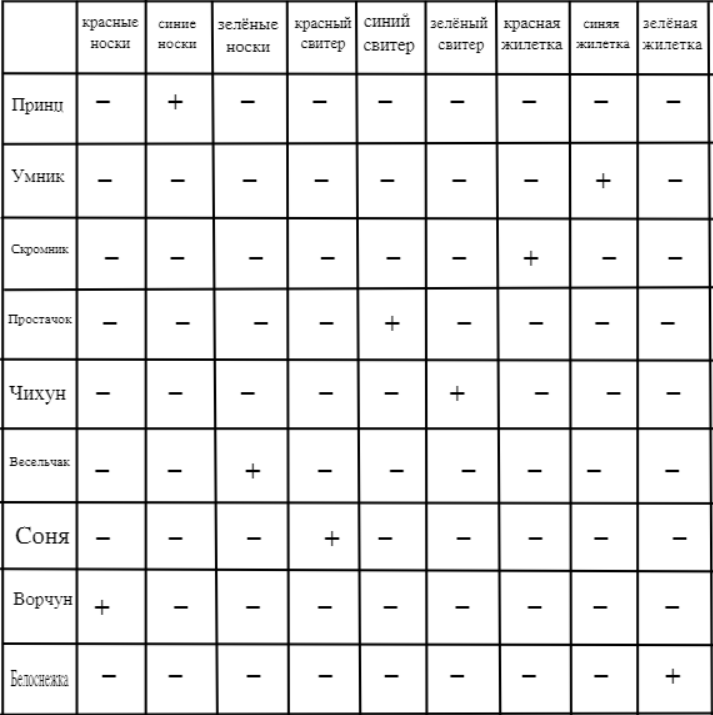
\includegraphics[scale=0.7]{pod.png}}
\end{figure}\\
Для решения этой задачи необходимо нарисовать таблицу и последовательно её заполнить. Принцу ставим $-$ во все клетки, кроме ЗЖ и СН. Умнику ставим $-$ во все клетки, кроме СН и СС. Скромнику ставим $-$ во все клетки, кроме КЖ, СС и СЖ. Простачку ставим $-$ во все клетки, кроме СС и СЖ. Чихуну и Весельчаку ставим $-$ в клетки КН, КС и КЖ. Соне ставим $-$ в КН. Весельчаку также ставим $-$ в СС и СЖ. Белоснежке ставим $+$ в ЗЖ, всем остальным в эту клетку $-$. Красные носки не могут достаться никому, кроме Ворчуна, ставим ему $+$ в эту клетку и $-$ в остальные. Зелёная жилетка досталась Белоснежке. поэтому Принц получил синие носки, ставим ему в эту клетку $+,$ всем остальным $-.$ Умнику остаётся только синяя жилетка, ставим ему в эту клетку $+,$ а всем остальным $-.$ Скромнику остаётся красная жилетка, ставим ему $+,$ а Соне $-.$ Простачку остаётся синий свитер, ставим ему $+,$ а остальным $-.$ Весельчаку остаются только зелёные носки, тогда Чихун должен получить зелёный свитер. Тогда Соне остаётся красный свитер и на этом распределение подарков окончено.\\
52. В каждой сотне цифра 4 встречается 11 раз в одном десятке (от .40 до .49) и по 1 разу во всех остальных, всего $11+9=20$ раз. Дополнительно сто цифр 4 встретятся в сотне от 400 до 499. Всего от 300 до 1100 содержится 8 сотен, а значит цифру 4 написали $8\cdot20+100=260$ раз.\\
53. Заметим, что $\cfrac{1}{k^2-1}=\cfrac{1}{(k-1)(k+1)}=\cfrac{1}{2}\left(\cfrac{1}{k-1}-\cfrac{1}{k+1}\right),$ поэтому
$\cfrac{1}{3}+\cfrac{1}{8}+\cfrac{1}{15}+\ldots+\cfrac{1}{n^2-1}=\cfrac{1}{2}\left(\cfrac{1}{1}-\cfrac{1}{3}+\cfrac{1}{2}-\cfrac{1}{4}+
\cfrac{1}{3}-\cfrac{1}{5}+\cfrac{1}{4}-\cfrac{1}{6}+\ldots+\cfrac{1}{n-2}-\cfrac{1}{n}+\cfrac{1}{n-1}-\cfrac{1}{n+1}\right)=
\cfrac{1}{2}\left(\cfrac{1}{1}+\cfrac{1}{2}-\cfrac{1}{n}-\cfrac{1}{n+1}\right)=$\\$=\cfrac{3n^2-n-2}{4n(n+1)}.$\\
54. Число $3^{4^5}=3^{2^{10}}=\left(3^{2^9}\right)^2$ является точным квадратом.\\
55. Пусть это число равно $n,$ тогда $n-2$ делится на 3 и на 23, а значит делится на 69. Поэтому минимальное значение $n$ равно $69+2=71.$\\
56. $633^{3^{72}}=633^{9^{36}}>633^{8^{36}}=633^{2^{108}}=633^{4^{54}}>632^{4^{54}}.$\\
57. $\cfrac{4n-23}{n-2}=\cfrac{4n-8-15}{n-2}=4-\cfrac{15}{n-2}.$ Для того, чтобы это число было натуральным, 15 должно делиться на $n-2.$ Если $n-2=15,$ то $n=17,$ а это число равно 3. Если $n-2=5,$ то $n=7,$ а это число равно 1. Если $n-2=3,$ то это число равно $-1$ и не является натуральным. Если $n-2=1,$ то это число равно $-11$ и не является натуральным. Если $n-2=-1,$ то $n=1,$ а это число равно 19. Таким образом, подходят только 1, 7 и 17.\\
58. Да, например так:
\begin{figure}[ht!]
\center{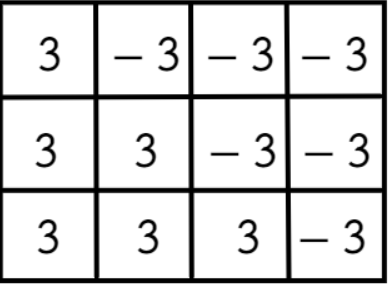
\includegraphics[scale=0.35]{tb.png}}
\end{figure}\\
59. $b^2+3b+2004=b^2+4b+4+2000-b=(b+2)^2+2000-b.$ При $b=2000$ это число равно $2002^2.$\\
60. Например, это можно сделать так:
\begin{figure}[ht!]
\center{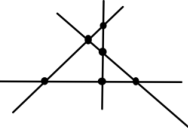
\includegraphics[scale=0.35]{aa.png}}
\end{figure}\\
61. Например, это можно сделать так:
\begin{figure}[ht!]
\center{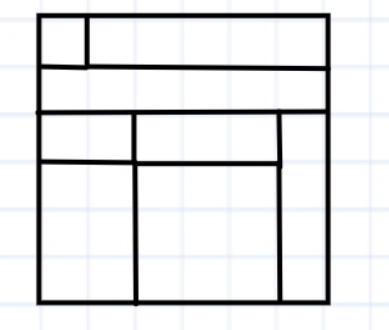
\includegraphics[scale=0.35]{aaa.png}}
\end{figure}\\
62. 3НОД(72, 80, 96)+$\frac{1}{2}$НОК(72, 80, 96)$=3\cdot8+\frac{1}{2}\cdot1440=744.$\\
63. Если число делится на 15, то оно делится на 3 и на 5. Если число делится на 5, его последняя цифра может быть только 0 или 5. Если последняя цифра равна 5, первая цифра равна $7-5=2,$ а вторая цифра должна быть такой, чтобы сумма цифр делилась на 3: 2, 5 или 8. Если последняя цифра равна 0, первая цифра равна $7-0=7,$ а вторая цифра должна быть такой, чтобы сумма цифр делилась на 3: 2, 5 или 8. Таким образом, подходят следующие числа: 225, 255, 285, 720, 750, 780.\\
64. $\left( \cfrac{1\cdot2\cdot4+2\cdot4\cdot8+\ldots+10\cdot20\cdot40}{1\cdot4\cdot5+2\cdot8\cdot10+\ldots+10\cdot40\cdot50}\right)^2=
\left( \cfrac{1\cdot2\cdot4\cdot(1+2\cdot2\cdot2+\ldots+10\cdot10\cdot10)}{1\cdot4\cdot5\cdot(1+2\cdot2\cdot2+\ldots+10\cdot10\cdot10)}\right)^2=$\\$=
\left( \cfrac{1\cdot2\cdot4}{1\cdot4\cdot5}\right)^2=\cfrac{4}{25}.$\\
65. Число 11 в любой степени заканчивается на 1. Число 9 в нечётных степенях заканчивается на 9. Последняя цифра степени двойки меняется по следующему правилу: 2, 4, 8, 6, 2, 4, ... Цикл состоит из 4 цифр, а 15 даёт остаток 3 при делении на 4, значит $2^{15}$ кончается на 8. Тогда последняя цифра числа $11^{50}+9^{35}-2^{15}$
равна $1+9-8=2.$\\
66. Пусть изначально число было равно  $\overline{ab},$ тогда $10b+a\geqslant3(10a+b),\ 10b+a\geqslant30a+3b,\ 7b\geqslant29a.$ Это неравенство может выполниться только при $a=1,\ b\in\{5,\ 6,\ 7,\ 8,\ 9\}$ или при $a=2,\ b=9.$ Всего подходит 6 чисел.\\
67. Пусть девятиклассники получили по $x$ тетрадей, а пятиклассники --- по $y.$ Тогда $12x+5y=120.$ Сумма делится на 12, как и первое слагаемое, значит второе слагаемое делится на 12, значит $y$ делится на 12. Если $y=24,$ то $x=0,$ что невозможно. Значит, $y=12,$ а тогда $x=5.$\\
68. Пусть $a\geqslant b\geqslant c$ и $a+b+c=80.$ Тогда сумма их попарных разностей равна $a-b+b-c+a-c=2(a-c).$ Наибольшее значение это выражение принимает тогда, когда разница между наибольшим и наименьшим из чисел максимальна, это достигается когда $a=77,\ b=2,\ c=1.$ Тогда это выражение равно $2\cdot(77-1)=152.$\\
69. Разложим на простые множители число 10472: $10472=2^3\cdot7\cdot11\cdot17.$ Числа 11 и 17 цифрами быть не могут, значит это делители самого числа. Тогда произведение цифр числа может быть равно 56, 28, 14, 7, 2 или 1. Небольшим перебором находим, что подходит только произведение цифр 56, само число при этом равно 187.\\
70. Пусть мы $a$ раз записали сообщение и $b$ раз удалили. В таком случае занято $500+198a-300b=2(250+99a-150b).$ Выражение $99a-150b$ всегда делится на 3, значит
$250+99a-150b$ даёт остаток 1 и таким образом не меньше 1. Тогда всего занято не менее 2 байт и полностью очистить память невозможно. Два байта можно получить, взяв $a=49,\ b=34.$\\
71. $8^7+2^{19}+4^9=2^{21}+2^{19}+2^{18}=2^{18}(2^3+2+1)=2^{18}\cdot11,$ что всегда делится на 11.\\
72. Пусть это число равно $x,$ тогда $x-1$ делится на каждое из чисел 2, 3, 4, 5, 6, а значит делится на 60. Первое делящееся на 7 число вида $60n+1$ равно 301.\\
73. Перечислим числа, при делении на которые 1000 даёт такой же остаток, как 1 или $-1:$ 3, 9, 27, 37, 111. При возведении в 1000 степень оно станет давать остаток 1 при делении на все эти числа, а значит после вычитания единицы будет на них делиться.\\
74. $k^2+(k+1)^2+(k+2)^2=k^2+k^2+2k+1+k^2+4k+4=3k^2+6k+5=3(k^2+2k+1)+2.$\\
75. Пусть $n=7k+3.$ Тогда $n^2+2n=(7k+3)^2+2(7k+3)=49k^2+42k+9+14k+6=49k^2+56k+15=7(7k^2+8k+2)+1.$\\
76. Переведём всё в копейки $15600+x$ должно делиться на 90, причём $0\leqslant x <100.$ Значит, $x$ должен делиться на 3 и на 10 (так как делится 15600), поэтому $x$ делится на 30. Из чисел 30, 60 и 90 подходит только 60, поэтому один ластик стоит $15660:90=174$ копейки или 1 рубль 74 копейки.\\
77. Разложим на простые множители: $12960=2^5\cdot3^4\cdot5.$ Чтобы число являлось квадратом целого числа, оно должно делиться только на чётные степени всех простых чисел, значит минимальное подходящее значение $T$ равно $2\cdot5=10.$\\
78. а) Пусть изначальное число равно $\overline{ab},$ тогда $10a+b+9=10b+a,\ 9a+9=9b,\ a+1=b.$ Значит, подходят числа 12, 23, 34, 45, 56, 67, 78, 89.\\
б) Пусть изначальное число равно $\overline{ab},$ тогда $10a+b-63=10b+a,\ 9a-63=9b,\ a-7=b.$ Значит, подходят числа 81, 92.\\
79. а) Самое большое простое число в этом ряду равно 157.\\
б) На 5 делятся числа от $95=5\cdot19$ до $160=5\cdot32,$ то есть $32-19+1=14$ чисел. На 25 делятся числа 100, 125 и 150, что даёт дополнительные три пятёрки. Также есть число 125, в множителях которого есть ещё одна дополнительная пятёрка. Значит, всего это произведение делится на $5^{18}.$\\
в) Двоек в этом произведении ещё больше (каждое второе число чётно), значит последние 18 цифр равны 0.\\
80. Число, кончающееся на 0, в любой степени кончается на 0. Последняя цифра степени числа, кончающегося на 7, изменяется следующим образом: 7, 9, 3, 1, 7, ...
Длина цикла равна 4, а 2008 делится на 4, значит эта степень кончается на 1. Таким образом, сумма этих чисел кончается на 1.\\
81. Раз Таня поймала окуня, Вика точно поймала щуку. Про Колю и Серёжу данных нет, так что каждый из них мог поймать плоту или леща.\\
82. Раз Вася поймал леща, плотву мог поймать только Толя. Катя с Семёно могли поймать окуня и щуку в любом порядке.\\
83. Пусть Вовочка получил $x$ пятёрок, тогда его средний балл равен $\cfrac{1+5x}{x+1}.$ Для того, чтобы средний балл стал равен 4,5, должно выполняться равенство
$\cfrac{1+5x}{x+1}=4,5,\ 1+5x=4,5x+4,5,\ 0,5x=3,5,\ x=7.$\\
84. Утверждение а) равносильно тому, что один фломастер стоит $15,86:4=3,965$ рубля. Утверждение б) равносильно тому, что один фломастер стоит $14,58:6=2,43$ рубля. Утверждение в) равносильно тому, что один фломастер стоит $18,68:8=2,335$ рубля. Так как тысячные доли рубля в расчётах участвовать не могут, верным является утверждение б).  Так как $5000:243=20$ (ост. 140), на 50 рублей можно купить 20 фломастеров.\\
85. а) Это верно, так как медиана, проведённая из прямого угла, равна половине гипотенузы.\\
б) $8^7-2^{18}=2^{21}-2^{18}=2^{18}\cdot(2^3-1)=2^{18}\cdot7,$ значит это утверждение также верно.\\
в) Это неверно, так как пары равных углов, прилежащих к равной стороне, может не найтись. Например, можно рассмотреть два равнобедренных прямоугольных треугольника (углы $90^\circ,\ 45^\circ,\ 45^\circ$), у первого из которых единице равен катет, а у второго --- гипотенуза.\\
86. Сумма всех чисел в строке равна $1+2+\ldots+37=(1+37)+(2+36)+\ldots+(18+20)+19=38\cdot18+19=703=37\cdot19.$ Сумма всех чисел, кроме последнего, делится на последнее число, а значит сумма вообще всех чисел тоже делится на последнее число. Но 703 делится только на 19, 37 и 1, а 37 и 1 написаны на первых двух местах. Значит, на последнем месте стоит число 19. На третьем месте стоит делитель числа $37+1=38,$ но числа 1 и 19 уже стоят на других местах, значит там стоит число 2.\\
87. Разложим на простые множители число $990:\ 990=2\cdot3^2\cdot5\cdot11.$ Значит $n$ должно быть как минимум 11, это значение подходит, так как до 11 есть множители 10 и 9.\\
88. Найдём самую маленькую возможную сумму семи троек: $1+2+3+\ldots+20+21=(1+21)+(2+20)+\ldots+(10+12)+11=22\cdot10+11=231.$ Теперь найдём самую большую возможную сумму семи различных чисел, не превосходящих 35: $35+34+33+32+31+30+29=224<231.$ Значит, семь троек обвести нельзя. Шесть троек обвести можно, например так:
$6+7+17=30,\ 5+8+18=31,\ 4+9+19=32,\ 3+10+20=33,\ 2+11+21=34,\ 1+12+22=35.$\\
89. Найдём самую маленькую возможную сумму девяти троек: $1+2+3+\ldots+20+27=(1+27)+(2+26)+\ldots+(15+13)+14=28\cdot13+14=378.$ Теперь найдём самую большую возможную сумму девяти различных чисел, не превосходящих 42: $42+41+40+39+38+37+36+35+34=342<378.$ Значит, девять троек обвести нельзя. Восемь троек обвести можно, например так:
$8+9+18=35,\ 7+10+19=36,\ 6+11+20=37,\ 5+12+21=38,\ 4+13+22=39,\ 3+14+23=40,\ 2+15+24=41,\ 1+16+25=42.$\\
90. НОК$(12,\ 70,\ 135) =$НОК$(2^2\cdot3,\ 2\cdot5\cdot7,\ 3^3\cdot5)=2^2\cdot3^3\cdot5\cdot7=3780.$\\
91. НОД$(2040,\ 4200)=$НОД$(2^3\cdot3\cdot5\cdot17,\ 2^3\cdot3\cdot5^2\cdot7)=2^3\cdot3\cdot5=120.$\\
92. НОК$(18,\ 30,\ 175)=$НОК$(2\cdot3^2,\ 2\cdot3\cdot5,\ 5^2\cdot7)=2\cdot3^2\cdot5^2\cdot7=3150.$\\
93. НОД$(2160,\ 10400)=$НОД$(2^4\cdot3^3\cdot5,\ 2^5\cdot5^2\cdot13)=2^4\cdot5=80.$\\
94. Число кратно 45 тогда и только тогда, когда оно кратно 5 и 9. Число кратно 5 тогда и только тогда, когда его последняя цифра 0 или 5. Значит, $b$ может быть равно 0 или 5. Число кратно 9 тогда и только тогда, когда сумма его цифр кратна 9. В первом случае $7+2+3+a+1+0=a+13$ кратно 9, тогда $a=5.$ Во втором случае
$7+2+3+a+1+5=a+18$ кратно 9, тогда $a=0$ или $a=9.$ Таким образом, подходят числа 723510, 723015 и 723915.\\
95. Число кратно 36 тогда и только тогда, когда оно кратно 4 и 9. Число кратно 4 тогда и только тогда, когда число, образованное двумя его последними цифрами, кратно 4. Значит, $b$ может быть равно 0, 4 или 8. Число кратно 9 тогда и только тогда, когда сумма его цифр кратна 9. В первом случае $6+5+a+8+0=a+19$ кратно 9, тогда $a=8.$ Во втором случае $6+5+a+8+4=a+23$ кратно 9, тогда $a=4.$ В третьем случае $6+5+a+8+8=a+27$ кратно 9, тогда $a=0$ или $a=9.$ Таким образом, подходят числа 65880, 65484, 65088 и 65988.\\
96. Число кратно 45 тогда и только тогда, когда оно кратно 5 и 9. Число кратно 5 тогда и только тогда, когда его последняя цифра 0 или 5. Значит, $b$ может быть равно 0 или 5. Число кратно 9 тогда и только тогда, когда сумма его цифр кратна 9. В первом случае $6+a+5+7+0=a+18$ кратно 9, тогда $a=0$ или $a=9.$ Во втором случае $6+5+a+7+5=a+23$ кратно 9, тогда $a=4.$ Таким образом, подходят числа 60570, 69570 и 64575.\\
97. Число кратно 36 тогда и только тогда, когда оно кратно 4 и 9. Число кратно 4 тогда и только тогда, когда число, образованное двумя его последними цифрами, кратно 4. Значит, $b$ может быть равно 0, 4 или 8.Число кратно 9 тогда и только тогда, когда сумма его цифр кратна 9. В первом случае $8+a+5+6+0=a+19$ кратно 9, тогда $a=8.$ Во втором случае $8+a+5+6+4=a+23$ кратно 9, тогда $a=4.$ В третьем случае $8+a+5+6+8=a+27$ кратно 9, тогда $a=0$ или $a=9.$ Таким образом, подходят числа 88560, 84564, 80568 и 89568.\\
98. Число $2x-20=2\cdot(x+5)-30$ кратно $x+5$ тогда и только тогда, когда 30 кратно $x+5.$ Так как число $x$ является натуральным, возможны случаи: $x+5=6,\ x=1,$ или $x+5=10,\ x=5,$ или $x+5=15,\ x=10,$ или $x+5=30,\ x=25.$\\
99. Число $k+11=k+13-2$ кратно $k+13$ тогда и только тогда, когда 2 кратно $k+13.$ Так как число $k$ является целым, возможны случаи: $k+13=2,\ k=-11,$ или $k+13=1,\ k=-12,$ или $k+13=-1,\ k=-14,$ или $k+13=-2,\ k=-15.$\\
100. Число $3x+7=3\cdot(x-2)+13$ кратно $x-2$ тогда и только тогда, когда 13 кратно $x-2.$ Так как число $x$ является натуральным, возможны случаи: $x-2=-1,\ x=1,\ x-2=1,\ x=3$ или $x-2=13,\ x=15.$\\
101. Число $2k-1=2\cdot(k+3)-7$ кратно $k+3$ тогда и только тогда, когда 7 кратно $k+3.$ Так как число $k$ является целым, возможны случаи: $k+3=7,\ k=4,$ или $k+3=1,\ k=-2,$ или $k+3=-1,\ k=-4,$ или $k+3=-7,\ k=-10.$\\
102. а) Да, $888:3=296.$\\
б) Нет, нечётное число не может делиться на чётное.\\
103. Пусть площадь их общей части равна $S,$ тогда площади областей равны $12^2-S=144-S$ и $15^2-S=225-S.$ Их разность равна $225-S-144+S=81.$\\
104. Так как знаменатели всей дробей не меньше 1, имеем соотношения $|x|\geqslant |z|, |y|\geqslant |x|,\ |z|\geqslant |y|,$ откуда
$|x|=|y|=|z|.$ Так как каждое неравенство должно обращаться в равенство, все знаменатели дробей равны 1 и $x=y=z=0.$\\
105. а) Да, 444444444 делится на 9, так как его сумма цифр $4\cdot9=36$ делится на 9.\\
б) Нет, нечётное число не может делиться на чётное.\\
106. Пусть площадь их общей части равна $S,$ тогда площади областей равны $11^2-S=121-S$ и $14^2-S=196-S.$ Их разность равна $196-S-121+S=75.$\\
107. Так как знаменатели всей дробей не меньше 1, имеем соотношения $|a|\geqslant |c|, |b|\geqslant |a|,\ |c|\geqslant |b|,$ откуда
$|a|=|b|=|c|.$ Так как каждое неравенство должно обращаться в равенство, все знаменатели дробей равны 1 и $a=b=c=0.$\\
108. $\cfrac{a^2-4b^2}{ab}=3,\ a^2-4b^2=3ab,\ a^2-3ab-4b^2=0,\ a^2+ab-4ab-4b^2=0,\ a(a+b)-4b(a+b)=0, (a+b)(a-4b)=0,\ a=4b$ (так как числа положительны). Тогда
$\cfrac{a^2+b^2}{ab}=\cfrac{a^2+16a^2}{4a^2}=\cfrac{17}{4},$ ч.т.д.\\
109. а) Попробуем подобрать пример, в котором в каждой группе по одному числу $x,\ y$ и $z.$ Они поменяются на $10x+3,\ 10y+7$ и $z.$ Тогда должно выполняться равенство $10x+3+10y+7+z=8x+8y+8z,\ 2x+2y+10=7z.$ Такие числа нетрудно подобрать, например $x=2,\ y=7, z=4.$\\
б) Пусть в первой группе $m$ чисел с суммой $x,$ во второй группе $n$ чисел с суммой $y,$ а в третьей группе числа с суммой $z.$ Тогда
$10x+3m+10y+7n+z=17x+17y+17z,\ 7x+7y+16z=3m+7n.$ Но так как все числа натуральны, $x\geqslant m$ и $y\geqslant n,$ поэтому левая часть всегда больше правой. Значит, в 17 раз сумма всех чисел увеличиться не могла.\\
110. Пусть $\cfrac{x}{2}=\cfrac{y}{3}=\cfrac{z}{4}=t,$ тогда $x=2t,\ t=3t,\ z=4t$ и $\cfrac{x+3y-z}{2x-3z}=\cfrac{2t+9t-4t}{4t-12t}=\cfrac{7t}{-8t}=-\cfrac{7}{8}.$\\
111. По количеству шариков понятно, что ребята стоят в следующем порядке: Коля, Петя, Женя, Сева. Тогда у Пети $32-21=11$ шариков, у Жени $21-13=8$ шариков, а у Севы $13-5=8$ шариков.\\
112. Пусть длинная сторона прямоугольника равна $a,$ а короткая $b,$ тогда имеем систему уравнений $\begin{cases} 3a+b=22,\\ 2a+2b=18.\end{cases}\Leftrightarrow
\begin{cases} 3a+b=22,\\ a+b=9.\end{cases}\Leftrightarrow
\begin{cases} 2a=13,\\ b=9-a.\end{cases}\Leftrightarrow
\begin{cases} a=6,5,\\ b=2,5.\end{cases}$ Тогда площадь прямоугольника равна $6,5\cdot2,5=16,25.$\\
113. $a+\cfrac{1}{b+\cfrac{1}{c}}=\cfrac{35}{11}=3\cfrac{2}{11},$ значит $a=3$ и $\cfrac{1}{b+\cfrac{1}{c}}=\cfrac{2}{11}.$ Тогда $b+\cfrac{1}{c}=\cfrac{11}{2}=5\cfrac{1}{2},$ откуда $b=5$ и $\cfrac{1}{c}=\cfrac{1}{2},$ поэтому $c=2.$ Таким образом, $abc=3\cdot5\cdot2=30.$\\
114. Заметим, что при натуральных $x$ и $y$ множители не обязательно должны быть натуральными. Рассмотрим все возможные разложения 6 на два целых множителя. Если $x-3=-6$ или $x-3=-3,$ то $x$ не является натуральным числом, что невозможно. Если $x-3=-2,$ то $x=1,$ а $y=(1-6:(-2)):2=2.$ Если $x-3=-1,$ то $x=2,$ а $y=(2-6:(-1)):2=4.$ Если $x-3=1,$ то $x=4,$ а $y=(4-6:1):2=-1,$ что невозможно. Если $x-3=2,$ то $x=5,$ а $y=(5-6:2):2=1.$ Если $x-3=3,$ то $x=6,$ а $y=(6-6:3):2=2.$ Если $x-3=6,$ то $x=9,$ а $y=(9-6:6):2=4.$ Итого $(x;y)\in\{(1;2),\ (2;4),\ (5;1),\ (6;2),\ (9;4)\}.$\\
115. Число 30303032 кончается на 2, а значит не может быть точным квадратом. Число 246801 имеет сумму цифр 21, а значит делится на 3, но не делится на 9, поэтому также не может быть точным квадратом. Число 56781234 делится на 2, но не делится на 4 (так как 34 не делится на 4), поэтому не может быть точным квадратом. Число 67812345 делится на 5, но не делится на 25 (так как 45 не делится на 25), значит и оно не может быть точным квадратом. Таким образом, точных квадратов среди приведённых чисел нет.\\
116. Пусть число имеет вид $\overline{abc}=100a+10b+c.$ Тогда $\overline{abc}-\overline{cba}=100a+10b+c-100c-10b-a=99(a-c)=198,\ a-c=2,\ a=c+2.$ Так как сумма квадратов цифр равна 101, получим равенство $b^2=101-a^2-c^2.$ Переберём все возможные значения буквы $c$ от 1 до 7. Если $c=1,$ то $a=3$ и $b^2=101-1-9=91,$ чего быть не может. Если $c=2,$ то $a=4$ и $b^2=101-4-16=81,\ b=9,$ то есть подходит число 492. Если $c=3,$ то $a=5$ и $b^2=101-9-25=67,$ чего быть не может. Если $c=4,$ то $a=6$ и $b^2=101-16-36=49,\ b=7$ то есть подходит число 674. Если $c=5,$ то $a=7$ и $b^2=101-25-49=27,$ чего быть не может. Если $c=6,$ то $a=8$ и $b^2=101-36-64=1,\ b=1,$ то есть подходит число 816. Если $c=7,$ то $a=9$ и $b^2=101-81-49=-29,$ чего быть не может. Таким образом, подходят только числа 492, 674, 816.\\
117. Обозначим искомое число буквой $x,$ тогда натуральное число $x-6$ должно делиться и на 7, и на 17. Так как числа 7 и 17 взаимно просты, наименьшее значение $x-6$ равно $7\cdot17=119,$ поэтому $x=119+6=125.$\\
118. Обозначим искомое число буквой $x,$ тогда натуральное число $x-4$ должно делиться и на 5, и на 19. Так как числа 5 и 19 взаимно просты, наименьшее значение $x-4$ равно $5\cdot19=95,$ поэтому $x=95+4=99.$\\
119. $\cfrac{1}{6}\cdot 7^{32}-(7+1)(7^2+1)(7^4+1)(7^8+1)(7^{16}+1)=\cfrac{7^{32}-(7-1)(7+1)(7^2+1)(7^4+1)(7^8+1)(7^{16}+1)}{6}=
\cfrac{7^{32}-(7^2-1)(7^2+1)(7^4+1)(7^8+1)(7^{16}+1)}{6}=\cfrac{7^{32}-(7^4-1)(7^4+1)(7^8+1)(7^{16}+1)}{6}=$\\$
\cfrac{7^{32}-(7^8-1)(7^8+1)(7^{16}+1)}{6}=\cfrac{7^{32}-(7^{16}-1)(7^{16}+1)}{6}=\cfrac{7^{32}-(7^{32}-1)}{6}=\cfrac{1}{6}.$\\
120. $\cfrac{1}{4}\cdot 5^{32}-(5+1)(5^2+1)(5^4+1)(5^8+1)(5^{16}+1)=\cfrac{5^{32}-(5-1)(5+1)(5^2+1)(5^4+1)(5^8+1)(5^{16}+1)}{4}=
\cfrac{5^{32}-(5^2-1)(5^2+1)(5^4+1)(5^8+1)(5^{16}+1)}{4}=\cfrac{5^{32}-(5^4-1)(5^4+1)(5^8+1)(5^{16}+1)}{4}=$\\$
\cfrac{5^{32}-(5^8-1)(5^8+1)(5^{16}+1)}{4}=\cfrac{5^{32}-(5^{16}-1)(5^{16}+1)}{4}=\cfrac{5^{32}-(5^{32}-1)}{4}=\cfrac{1}{4}.$\\
121. Если $2n-1>n-5>0,$ то дробь точно не может быть целой, так как является правильной. Значит, достаточно разобрать случаи $n\in\{1; 2; 3; 4; 5\}.$ При $n=1$ дробь равна $\cfrac{1-5}{2\cdot1-1}=-4,$ это значение подходит. При $n=2$ дробь равна $\cfrac{2-5}{2\cdot2-1}=-1,$ это значение тоже подходит.
При $n=3$ дробь равна $\cfrac{3-5}{2\cdot3-1}=-0,4,$ это значение не подходит. При $n=4$ дробь равна $\cfrac{4-5}{2\cdot4-1}=-\cfrac{1}{7},$ это значение тоже не подходит. При $n=5$ дробь равна $\cfrac{5-5}{2\cdot5-1}=0,$ это значение подходит. Таким образом, дробь может быть равна $-4,\ -1$ и 0.\\
122. Если $2n-5>n-1>0,$ то дробь точно не может быть целой, так как является правильной. Значит, достаточно разобрать случаи $n\in\{1; 2; 3; 4\}.$ При $n=1$ дробь равна $\cfrac{1-1}{2\cdot1-5}=0,$ это значение подходит. При $n=2$ дробь равна $\cfrac{2-1}{2\cdot2-5}=-1,$ это значение тоже подходит.
При $n=3$ дробь равна $\cfrac{3-1}{2\cdot3-5}=2,$ это значение также подходит. При $n=4$ дробь равна $\cfrac{4-1}{2\cdot4-5}=1,$ это значение тоже подходит. Таким образом, дробь может быть равна $-2,\ -1,\ 0$ и 1.\\
123. а) Да, можно, например так: 2 сосиски режем на части $3+3+3+5,$ 4 сосиски режем на части $3+3+4+4$ и 6 сосисок режем на части $5+5+4.$ Тогда сосисок для котят будет $3\cdot2+2\cdot4=14,$ сосисок для кошек будет $2\cdot4+1\cdot6=14,$ и сосисок для котов будет $1\cdot2+2\cdot6=14.$\\
б) Из сосиски длиной 11 см не получится вырезать две части для котов (тогда останется 1 см, который никому не нужен), поэтому по 1 части для котов придётся вырезать из каждой сосиски, кроме одной. Но тогда из остатка нельзя вырезать часть для кошки, так как тогда останутся 2 см, которые никому не нужны, а значит разделить сосиски таким образом не получится.\\
124. а) Да, можно, например так: 1 сосиску режем на части $3+3+2+2+2+2,$ 4 сосиски режем на части $5+3+3+3$ и 5 сосисок режем на части $5+5+2+2.$ Тогда сосисок для котят будет $4\cdot1+2\cdot5=14,$ сосисок для кошек будет $2\cdot1+4\cdot3=14,$ и сосисок для котов будет $1\cdot4+2\cdot5=14.$\\
б) Из сосиски длиной 11 см не получится вырезать две части для котов (тогда останется 1 см, который никому не нужен), поэтому по 1 части для котов придётся вырезать из каждой сосиски. Но тогда их будет максимум $10<11,$ значит поделить сосиски таким образом невозможно.
\newpage
\section{геометрия решения}
1. \begin{figure}[ht!]
\center{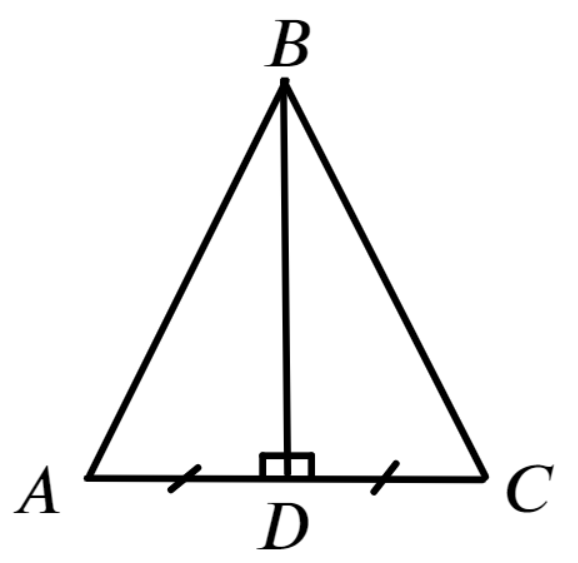
\includegraphics[scale=0.35]{g1.png}}
\end{figure}\\
$\left.\begin{array}{l}AD=DC\text{ т.к. }BD\text{ медиана,}\\
\angle ADB=\angle CDB=90^\circ \text{ т.к. }BD\text{ высота,}\\
BD - \text{ общая.}   \end{array}\right\}\Rightarrow
\Delta ADB=\Delta CDB\text{ по I признаку }\Rightarrow BA=BC\text{ ч.т.д.} $\\
2.  \begin{figure}[ht!]
\center{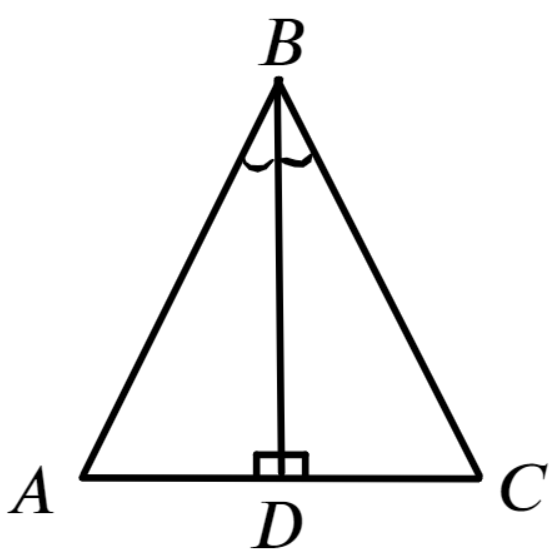
\includegraphics[scale=0.35]{g2.png}}
\end{figure}\\
$\left.\begin{array}{l}\angle ABD=\angle CBD\text{ т.к. }BD\text{ биссектриса,}\\
\angle ADB=\angle CDB=90^\circ \text{ т.к. }BD\text{ высота,}\\
BD - \text{ общая.}   \end{array}\right\}\Rightarrow
\Delta ADB=\Delta CDB\text{ по II признаку }\Rightarrow BA=BC\text{ ч.т.д.} $\\
3. \begin{figure}[ht!]
\center{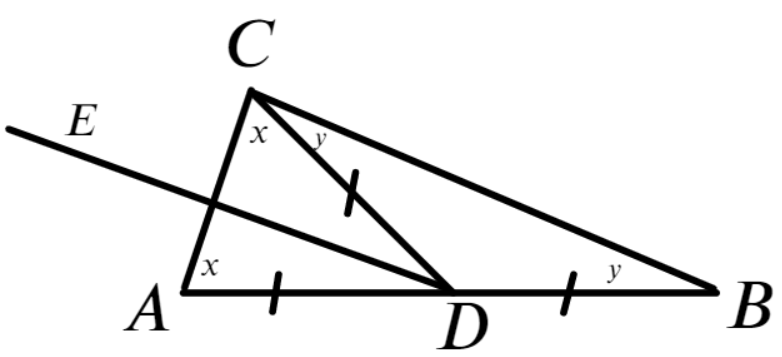
\includegraphics[scale=0.35]{g3.png}}
\end{figure}\\
Треугольники $ADC$ и $BDC$ являются равнобедренными, значит в них углы при основании равны. Обозначим $\angle CAD=\angle ACD=x,\ \angle DBC=\angle BDC=y.$ Тогда выразим сумму углов треугольника $ABC:\ 2x+2y=180^\circ,\ x+y=90^\circ\Rightarrow BC \perp AC\Rightarrow DE\perp AC,$ ч.т.д. (т.к. $DE\parallel BC$)\\
4. \begin{figure}[ht!]
\center{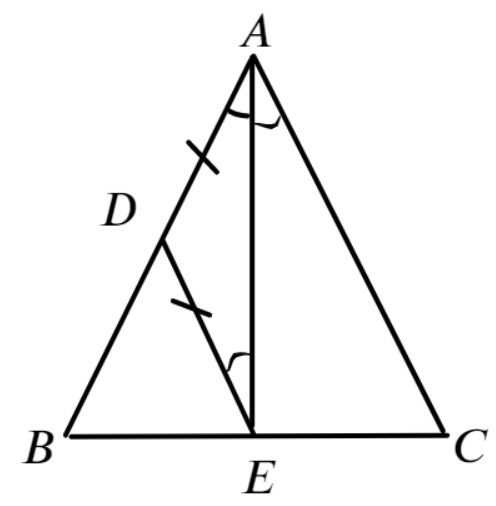
\includegraphics[scale=0.35]{g4.png}}
\end{figure}\\
Треугольник $DAE$ является равнобедренным $(AD=DE),$ значит углы при основании равны: $\angle DAE=\angle DEA.$ Прямые $DE$ и $AC$ параллельны, $AE$ секущая, значит  $\angle DEA=\angle EAC$ как накрест лежащие. Поэтому $\angle DAE=\angle EAC,$ то есть $AE$ является биссектрисой угла $A,$ а поэтому и высотой (так как треугольник $ABC$ равнобедренный). Значит, $AE\perp BC.$\\
5. \begin{figure}[ht!]
\center{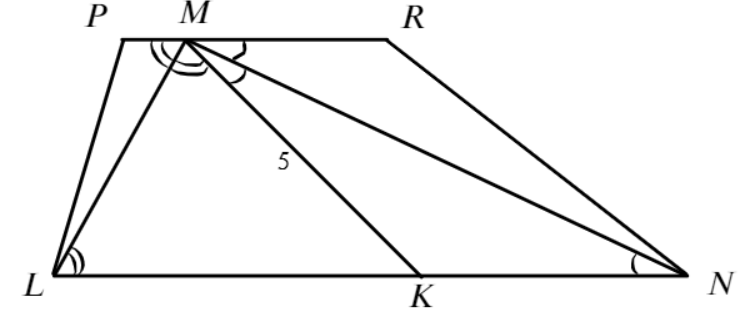
\includegraphics[scale=0.35]{g5.png}}
\end{figure}\\
Прямые $PR$ и $LN$ параллельны, а $LM$ и $MN$ --- секущие, значит $\angle PML = \angle MLK,$  $\angle RMN= \angle MNK$ как накрест лежащие. $MN$ и $ML$ являются биссектрисами, поэтому $\angle PML = \angle LMK,$ $ \angle RMN= \angle NMK.$ Поэтому у треугольников $LMK$ и $NMK$ равны углы при основаниях, а значит они равнобедренные и $LK=MK=5,\ KN=MK=5,$ откуда $LN=LK+KN=5+5=10.$\\
6. \begin{figure}[ht!]
\center{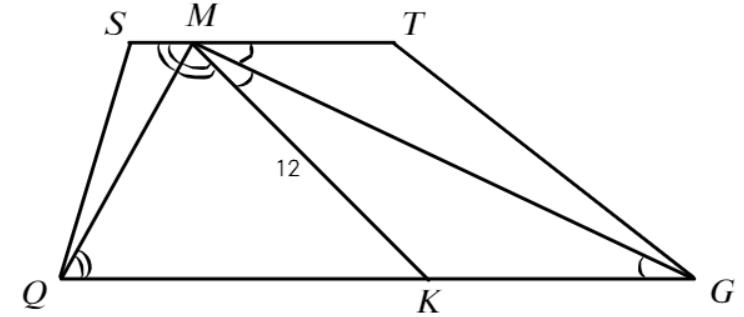
\includegraphics[scale=0.35]{g6.png}}
\end{figure}\\
Прямые $ST$ и $QG$ параллельны, а $QM$ и $MK$ --- секущие, значит $\angle SMQ = \angle MQK,$  $\angle TMG= \angle MGK$ как накрест лежащие. $MG$ и $MQ$ являются биссектрисами, поэтому $\angle SMQ = \angle QMK,$ $ \angle TMG= \angle GMK.$ Поэтому у треугольников $QMK$ и $GMK$ равны углы при основаниях, а значит они равнобедренные и $QK=MK=12,\ KG=MK=12,$ откуда $QG=QK+KG=12+12=24.$\\
7. \begin{figure}[ht!]
\center{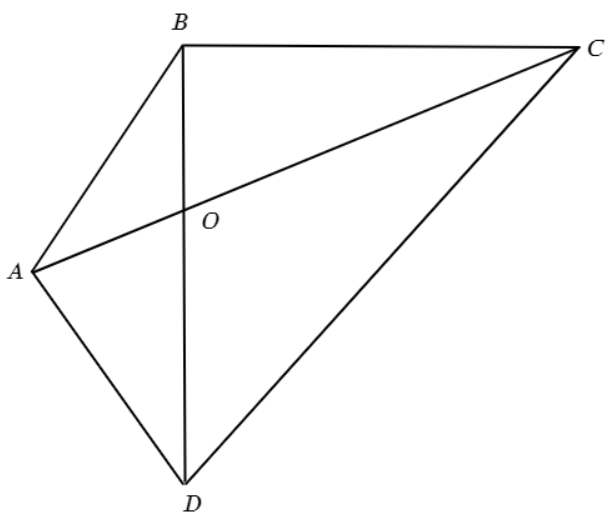
\includegraphics[scale=0.35]{g7.png}}
\end{figure}\\
Запишем четыре неравенства треугольника: $AO+OD>AD,\ BO+AO>AB,\ BO+OC>BC,\ OC+OD>CD.$ После сложения этих неравенств получим $2AO+2OC+2BO+2OD>AB+BC+CD+AD,\ 2(AC+BD)>P,\ AC+BD>\cfrac{P}{2},$ ч.т.д.\\
8. \begin{figure}[ht!]
\center{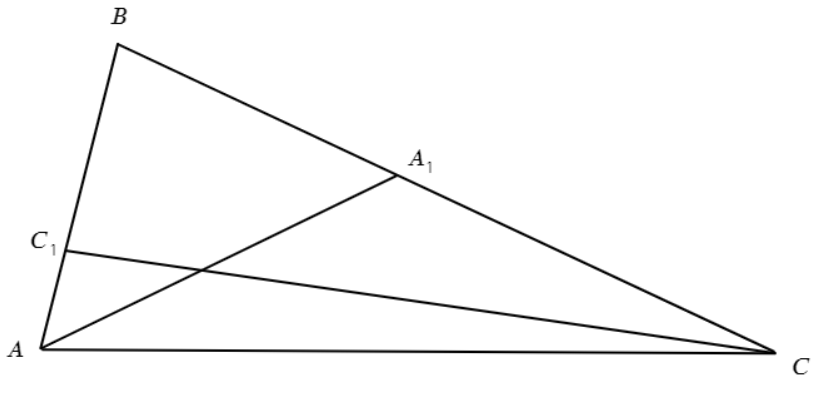
\includegraphics[scale=0.35]{g8.png}}
\end{figure}\\
Запишем четыре неравенства треугольника: $AB+BA_1>AA_1,\ AC+CA_1>AA_1,\ BC+BC_1>CC_1,\ AC+AC_1>CC_1.$ После сложения этих неравенств получим
$AB+AC+BC+AC+BA_1+CA_1+BC_1+AC_1>2AA_1+2CC_1,\ 2P>2AA_1+2CC_1,\ P>AA_1+CC_1,$ ч.т.д.\\
9. \begin{figure}[ht!]
\center{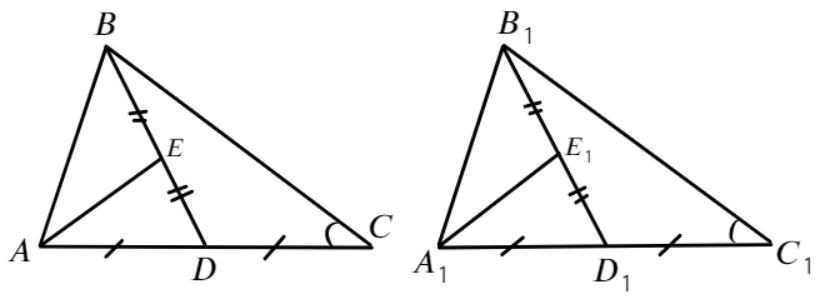
\includegraphics[scale=0.35]{g9.png}}
\end{figure}\\
$\left.\begin{array}{l}BC=B_1C_1,\\
\angle C=\angle C_1,\\
DC=\frac{1}{2}AC=\frac{1}{2}A_1C_1=D_1C_1  \end{array}\right\}\Rightarrow
\Delta BDC=\Delta B_1D_1C_1\text{ по I признаку }\Rightarrow $\\$\Rightarrow ED=\frac{1}{2}BD=\frac{1}{2}B_1D_1=E_1D_1,\ \angle EDA=180^\circ-\angle BDC=180^\circ-\angle B_1D_1C_1=\angle E_1D_1A_1.$\\
$\left.\begin{array}{l}AD=\frac{1}{2}AC=\frac{1}{2}A_1C_1=A_1D_1,\\
\angle EDA=\angle E_1D_1A_1,\\
ED=E_1D_1  \end{array}\right\}\Rightarrow \Delta AED=\Delta A_1E_1D_1\text{ по I признаку }\Rightarrow AE=A_1E_1,$ ч.т.д.\\
10. \begin{figure}[ht!]
\center{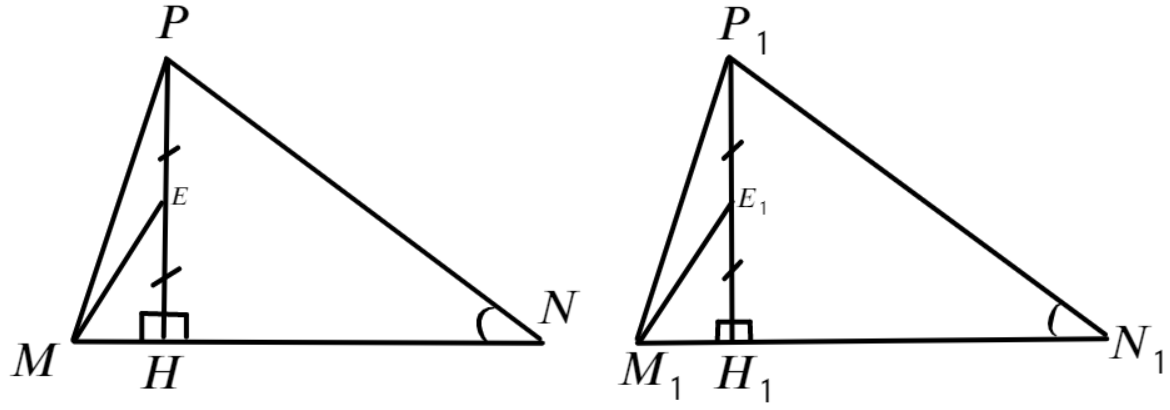
\includegraphics[scale=0.35]{g10.png}}
\end{figure}\\
$\left.\begin{array}{l}PN=P_1N_1,\\
\angle N=\angle N_1. \end{array}\right\}\Rightarrow
\Delta PNH=\Delta P_1N_1H_1\text{ по гипотенузе и острому углу }\Rightarrow $\\$\Rightarrow EH=\frac{1}{2}PH=\frac{1}{2}P_1H_1=E_1H_1,\ MH=MN-HN=M_1N_1-H_1N_1=M_1H_1.$\\
$\left.\begin{array}{l}EH=E_1H_1,\\
MH=M_1H_1  \end{array}\right\}\Rightarrow \Delta MEH=\Delta M_1E_1H_1\text{ по двум катетам }\Rightarrow ME=M_1E_1,$ ч.т.д.\\
11. \begin{figure}[ht!]
\center{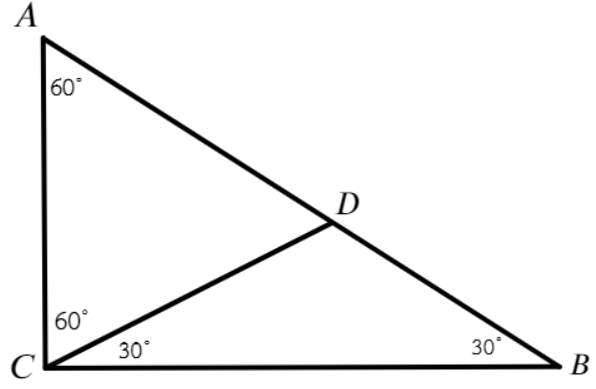
\includegraphics[scale=0.35]{g11.png}}
\end{figure}\\
Треугольник $ACD$ равносторонний, значит все его углы равны $60^\circ.$ Тогда $\angle DCB=\angle C-\angle ACD=90^\circ-60^\circ=30^\circ,\ \angle DBC=180^\circ-\angle A-\angle C=180^\circ-60^\circ-90^\circ=30^\circ.$ Поэтому в треугольнике $BCD$ равны углы при основании $BC$ и он является равнобедренным, ч.т.д.\\
12. \begin{figure}[ht!]
\center{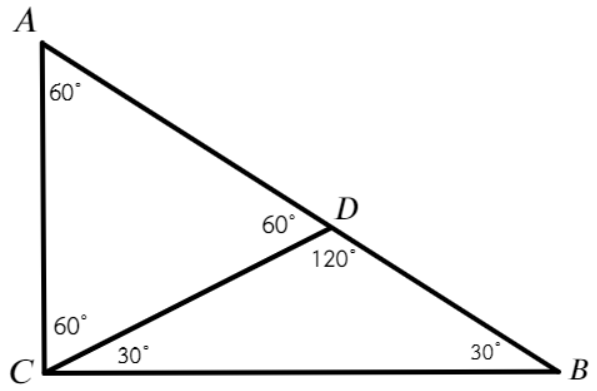
\includegraphics[scale=0.35]{g12.png}}
\end{figure}\\
Треугольник $BCD$ равнобедренный с углом $120^\circ,$ значит углы при основании $BC$ равны $(180^\circ-120^\circ):2=30^\circ.$ Тогда $\angle ACD=\angle C-\angle DCB=90^\circ-30^\circ=60^\circ,\ \angle CAD=180^\circ-\angle C-\angle B=180^\circ-90^\circ-30^\circ=60^\circ,\ \angle CDA=180^\circ-\angle CDB=180^\circ-120^\circ=60^\circ,$
значит треугольник $ACD$ является равносторонним, ч.т.д.\\
13. \begin{figure}[ht!]
\center{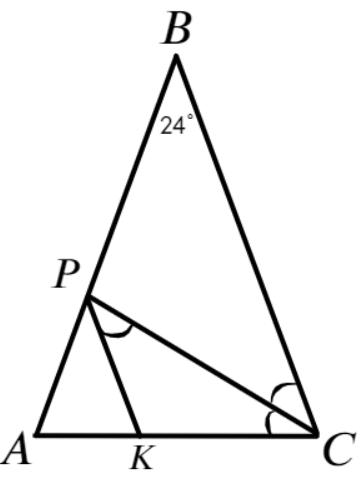
\includegraphics[scale=0.35]{g13.png}}
\end{figure}\\
Треугольник $ABC$ равнобедренный, поэтому $\angle C=(180^\circ-24^\circ):2=78^\circ.$ Так как $CP$ является биссектрисой, $\angle ACP=\angle BCP=78^\circ:2=39^\circ.$ Прямые $BC$ и $PK$ параллельны, $CP$ секущая, поэтому углы $KPC$ и $BCP$ равны как накрест лежащие, откуда $\angle KPC=39^\circ.$\\
14. \begin{figure}[ht!]
\center{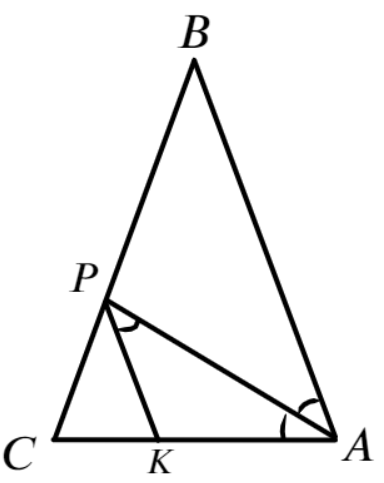
\includegraphics[scale=0.35]{g14.png}}
\end{figure}\\
Треугольник $ABC$ равнобедренный, поэтому $\angle A=\angle C =72^\circ.$ Так как $AP$ является биссектрисой, $\angle PAC=\angle PAB=72^\circ:2=36^\circ.$ Прямые $AB$ и $PK$ параллельны, $AP$ секущая, поэтому углы $KPA$ и $PAB$ равны как накрест лежащие, откуда $\angle KPA=36^\circ.$\\
15. Да, существует. На картинке изображён один из возможных примеров.
\begin{figure}[ht!]
\center{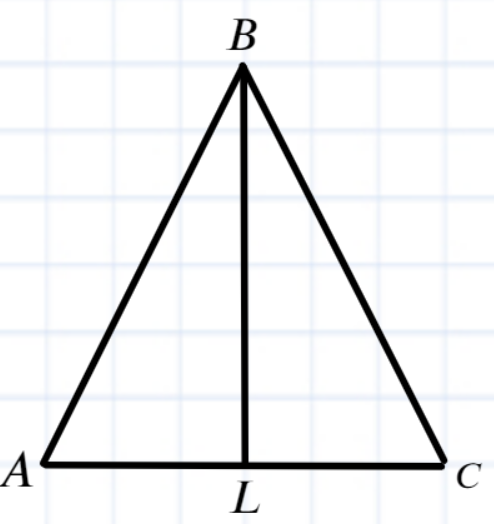
\includegraphics[scale=0.35]{g15.png}}
\end{figure}\\
16. Нет, неверно. На картинке изображён один из возможных примеров.
\begin{figure}[ht!]
\center{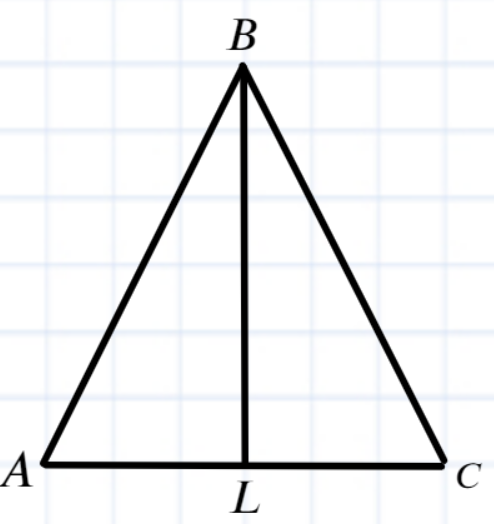
\includegraphics[scale=0.35]{g15.png}}
\end{figure}\newpage\noindent
17. \begin{figure}[ht!]
\center{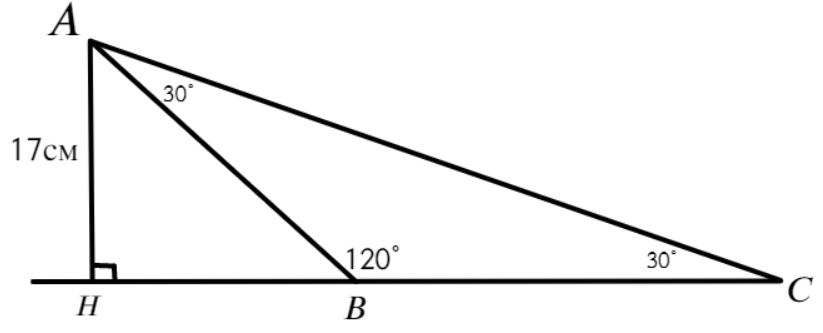
\includegraphics[scale=0.35]{g17.png}}
\end{figure}\\
Углом в $120^\circ$ может быть только угол при вершине, тогда углы при основании треугольника равны $(180^\circ-120^\circ):2=30^\circ.$ Поэтому в прямоугольном треугольнике $AHC$ катет $AH$ лежит напротив угла $30^\circ,$ а значит равен половине гипотенузы $AC.$ Таким образом, $AC=2\cdot17=34$ см.\\
18. \begin{figure}[ht!]
\center{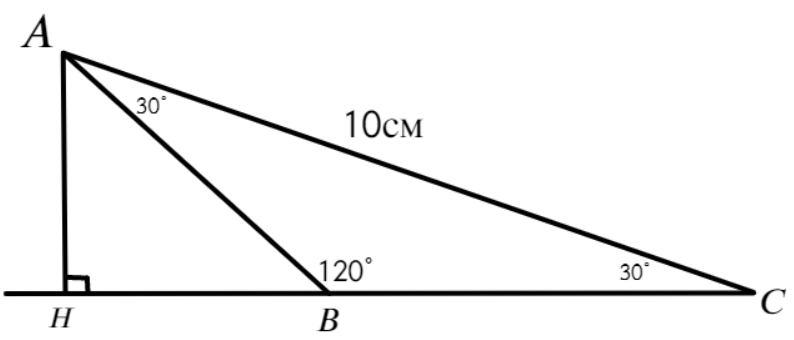
\includegraphics[scale=0.35]{g18.png}}
\end{figure}\\
Углом в $120^\circ$ может быть только угол при вершине, тогда углы при основании треугольника равны $(180^\circ-120^\circ):2=30^\circ.$ Поэтому в прямоугольном треугольнике $AHC$ катет $AH$ лежит напротив угла $30^\circ,$ а значит равен половине гипотенузы $AC.$ Таким образом, $AH=10:2=5$ см.\\
19. Да, можно. На картинке изображён один из возможных примеров.
\begin{figure}[ht!]
\center{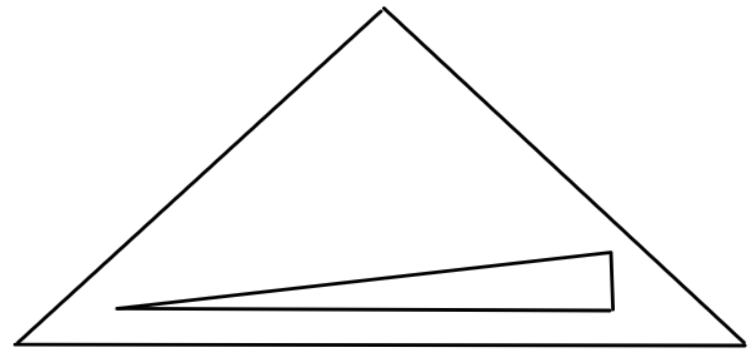
\includegraphics[scale=0.35]{g19.png}}
\end{figure}\\
20. Да, можно. Представим, что две вершины внутреннего треугольника и левая вершина внешнего треугольника лежат на окружности радиусом 566 с центром в нижней вершине.
\begin{figure}[ht!]
\center{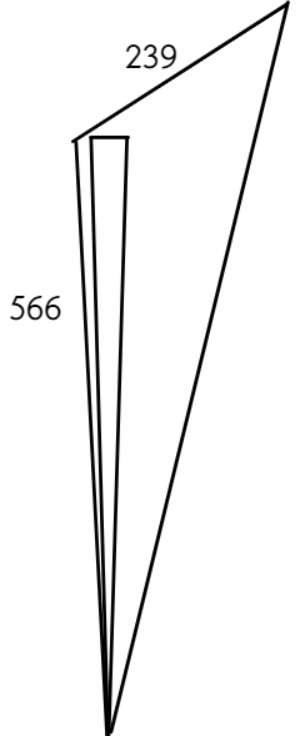
\includegraphics[scale=0.35]{g20.png}}
\end{figure}\newpage\noindent
21. \begin{figure}[ht!]
\center{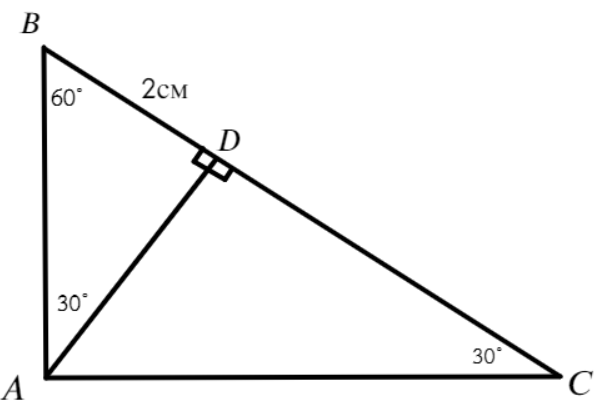
\includegraphics[scale=0.35]{g21.png}}
\end{figure}\\
$\angle BAD=\angle C=90^\circ-\angle B=90^\circ-60^\circ=30^\circ.$ В прямоугольном треугольнике $ABD$ катет $DB$ лежит напротив угла в $30^\circ,$ а значит гипотенуза $AB=2\cdot2=4$см. В прямоугольном треугольнике $ABC$ катет $AB$ лежит напротив угла в $30^\circ,$ значит гипотенуза $BC=2\cdot4=8$см. Таким образом, $DC=BC-DB=8-2=6$см.\\
22. \begin{figure}[ht!]
\center{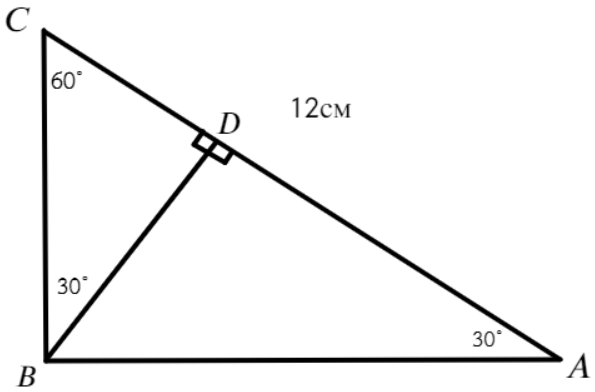
\includegraphics[scale=0.35]{g22.png}}
\end{figure}\\
$\angle C=90^\circ-\angle A=90^\circ-30^\circ=60^\circ,\ \angle CBD=90^\circ-\angle C=90^\circ-60^\circ=30^\circ.$ В прямоугольном треугольнике $ABC$ катет $BC$ лежит напротив угла в $30^\circ,$ а значит $BC=AC:2=12:2=6$см. В прямоугольном треугольнике $BCD$ катет $CD$ лежит напротив угла в $30^\circ,$ а значит $CD=BC:2=6:2=3$см. Тогда $DA=AC-CD=12-3=9$см.\\
23. Для стороны есть 2 варианта: она может быть боковой стороной или основанием. Для угла также есть 2 варианта: он может быть углом при вершине или при основание. Таким образом, существует $2\cdot2=4$ неравных между собой треугольников.\\
24. Если у равнобедренного треугольника один из углов равен $60^\circ,$ остальные его углы тоже равны $60^\circ,$ а значит он является равносторонним. Так как длина стороны задана, такой треугольник существует только один.\\
25. \begin{figure}[ht!]
\center{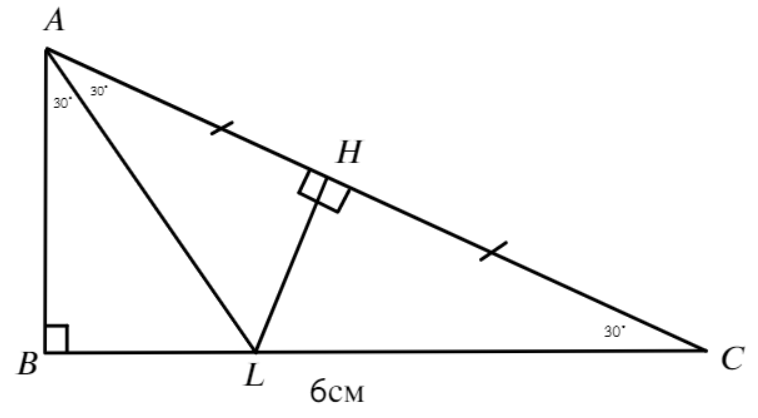
\includegraphics[scale=0.35]{g25.png}}
\end{figure}\\
Так как $AL$ является биссектрисой, $\angle BAL=\angle LAC=60^\circ:2=30^\circ.$ Угол $C$ также равен $90^\circ-\angle A=90^\circ-60^\circ=30^\circ.$ В прямоугольных треугольниках $LAH$ и $LCH$ катет $LH$ лежит напротив угла в $30^\circ,$ а значит $AL=LC=2LH.$ В прямоугольном треугольнике $ABL$ катет $BL$ лежит напротив угла
в $30^\circ,$ а значит $BL=AL:2=2LH:2=LH.$ Таким образом, $BC=BL+LC=LH+2LH=3LH=6$см, откуда $LH=6:3=2$см.\newpage\noindent
26. \begin{figure}[ht!]
\center{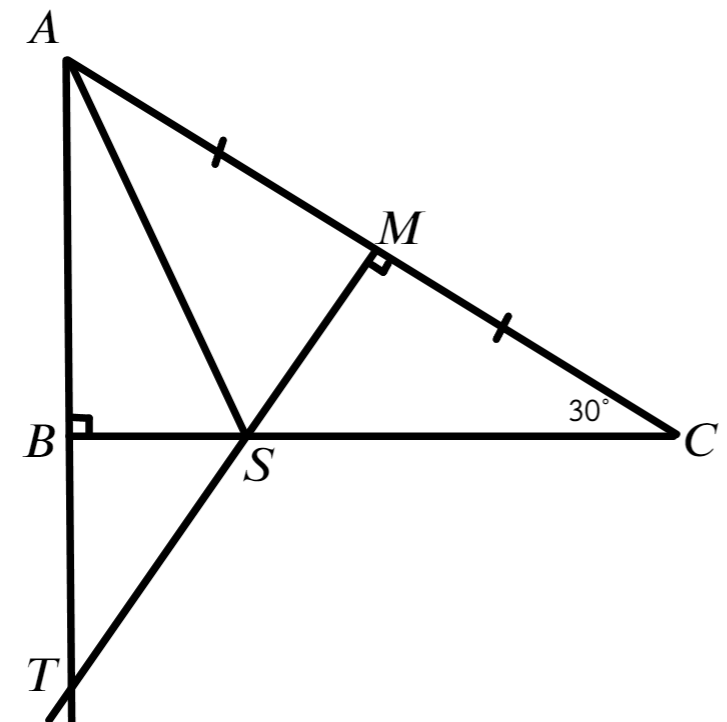
\includegraphics[scale=0.35]{g26.png}}
\end{figure}\\
$\angle C=90^\circ-\angle A=90^\circ-60^\circ=30^\circ.$ Пусть $MT$ пересекает сторону $BC$ в точке $S.$ Так как в треугольнике $ASC$ высота совпала с медианой, он является равнобедренным, поэтому $\angle SAC=\angle C=30^\circ.$ Тогда $\angle BAS=\angle A-\angle SAC=60^\circ-30^\circ=30^\circ.$ В прямоугольных треугольниках $SAM$ и $SCM$ катет $MS$ лежит напротив угла в $30^\circ,$ а значит $AS=SC=2MS.$ В прямоугольном треугольнике $ABS$ катет $BS$ лежит напротив угла
в $30^\circ,$ а значит $BS=AS:2=2MS:2=MS.$ Таким образом, $BC=BS+SC=MS+2MS=3MS=3$см, откуда $MS=3:3=1$см. Из треугольника $TAM$ найдём $\angle ATM=90^\circ-60^\circ=30^\circ.$ В прямоугольном треугольнике $TBS$ катет $BS$ лежит напротив угла в $30^\circ,$ значит $ST=2BS=2\cdot1=2$см. Таким образом, $MT=MS+ST=1+2=3$см.\\
27. \begin{figure}[ht!]
\center{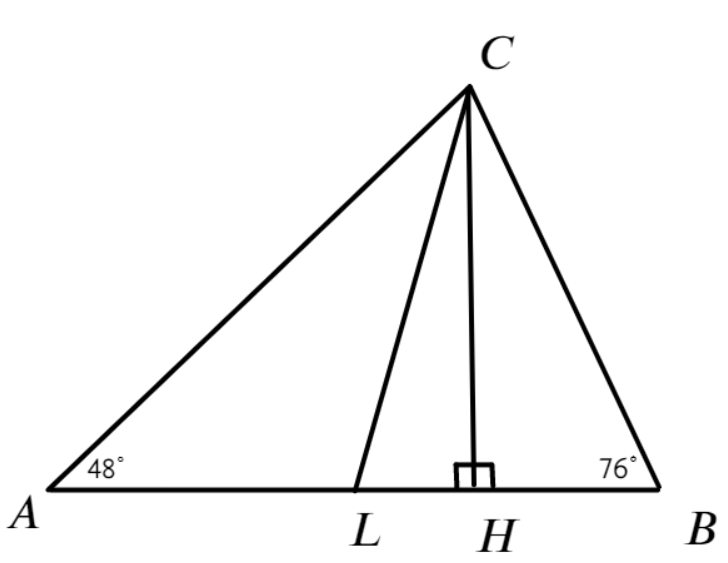
\includegraphics[scale=0.35]{g27.png}}
\end{figure}\\
$\angle C=180^\circ-\angle A-\angle B=180^\circ-48^\circ-76^\circ=56^\circ.$ Пусть $CH$ высота, а $CL$ --- биссектриса. Тогда $\angle BCH=90^\circ-76^\circ=14^\circ,$ а $\angle BCL=56^\circ:2=28^\circ.$ Таким образом, $\angle LCH=\angle BCL- \angle BCH=28^\circ-14^\circ=14^\circ.$\\
28. \begin{figure}[ht!]
\center{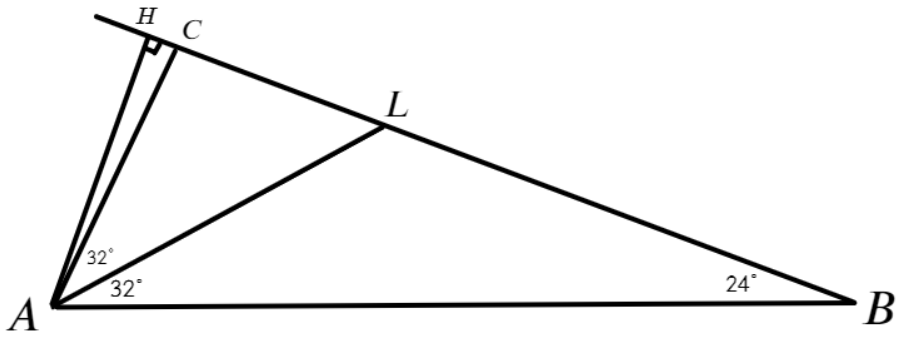
\includegraphics[scale=0.35]{g28.png}}
\end{figure}\\
$\angle C=180^\circ-\angle A-\angle B=180^\circ-64^\circ-24^\circ=92^\circ.$ Так как $\angle C>90^\circ,$ высота из точки $A$ падает на продолжение стороны $BC.$   Пусть $AH$ высота, а $AL$ --- биссектриса. Тогда $\angle CAH=90^\circ-\angle HCA=90^\circ-(180^\circ-\angle C)=90^\circ-88^\circ=2^\circ,$ а $\angle CAL=64^\circ:2=32^\circ.$ Таким образом, $\angle LAH=\angle CAL+ \angle CAH=32^\circ+2^\circ=34^\circ.$\newpage\noindent
29. \begin{figure}[ht!]
\center{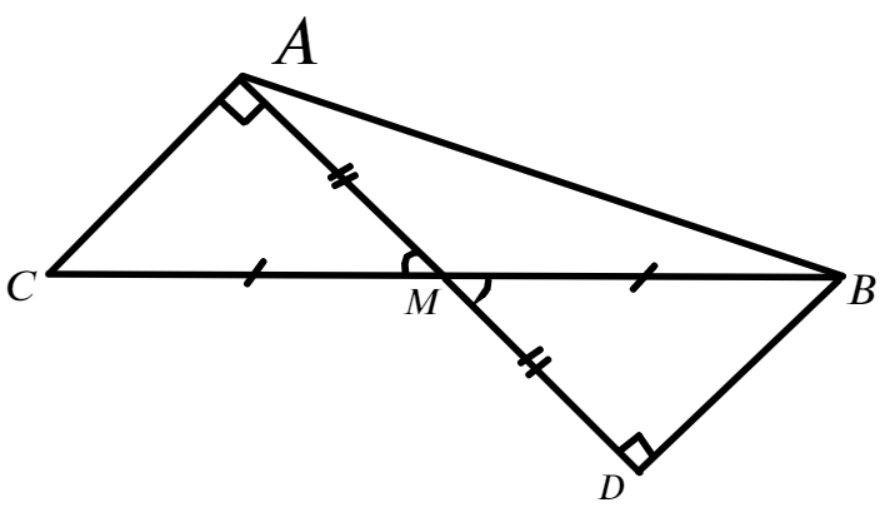
\includegraphics[scale=0.35]{g29.png}}
\end{figure}\\
Сделаем стандартное дополнительное построение: продлим медиану $AM$ на свою длину: $AM=MD.$ Тогда $\left.\begin{array}{l}AM=MD\text{ по построению},\\
 CM=MB\text{ ($AM$ --- медиана)},\\ \angle BMD=\angle CMA\text{ (вертикальные).}\end{array}\right\}\Rightarrow
\Delta BMD=\Delta CMA\text{ по I признаку}\Rightarrow AC=BD$ и $\angle BDM=\angle CAM=90^\circ.$ Треугольник $BAD$ является прямоугольным и в нём $AB=2AC=2BD,$ значит катет $BD$ лежит напротив угла в $30^\circ,$ поэтому $\angle BAM=30^\circ.$ Таким образом, $\angle BAC=90^\circ+30^\circ=120^\circ.$\\
30. \begin{figure}[ht!]
\center{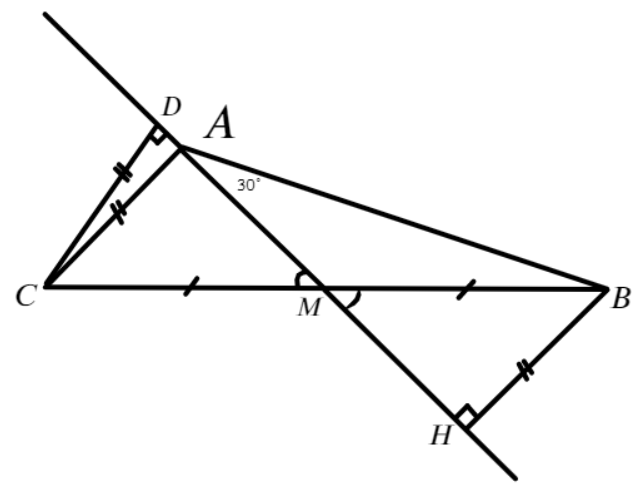
\includegraphics[scale=0.35]{g30.png}}
\end{figure}\\
Сделаем дополнительное построение: опустим из точки $B$ перпендикуляр $BH$ на продолжение медианы $AM.$ Треугольник $ABH$ является прямоугольным и катет $BH$ лежит напротив угла в $30^\circ,$ поэтому $BH=\frac{1}{2}AB=AC.$ Теперь опустим перпендикуляр $CD$ из точки $C$ на прямую $AM.$ Углы $DMC$ и $HMB$ являются вертикальными, $CM=MB$ (так как $AM$ медиана), значит прямоугольные треугольники $DMC$ и $HMB$ равны по гипотенузе и острому углу, поэтому $CD=BH=AC.$ Но тогда в прямоугольном треугольнике $CDA$ катет равен гипотенузе, что невозможно, значит точка $D$ совпадает с точкой $A$ и $\angle CAM=90^\circ.$ Таким образом, $\angle BAC=90^\circ+30^\circ=120^\circ.$\newpage
\noindent31. \begin{figure}[ht!]
\center{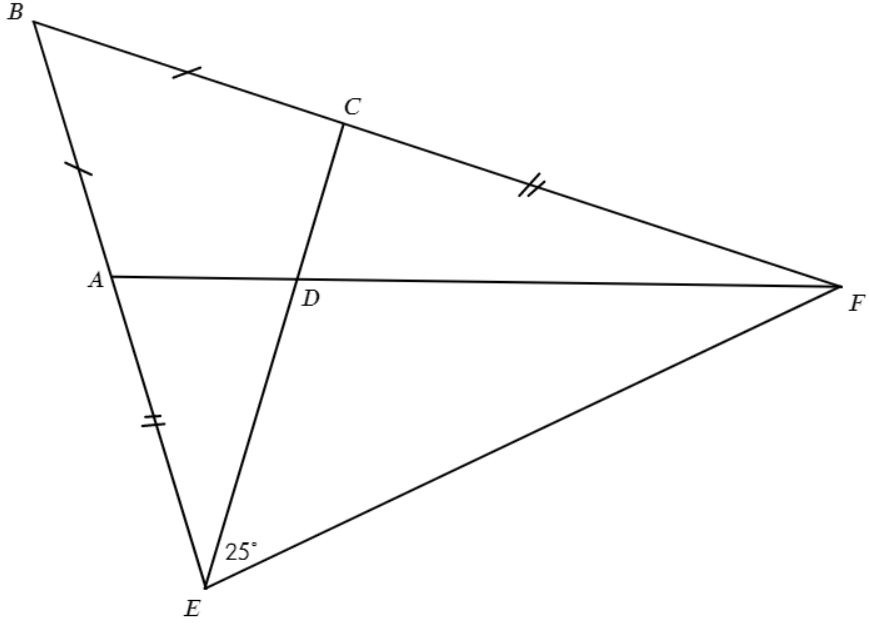
\includegraphics[scale=0.35]{g31.png}}
\end{figure}\\
Заметим, что $AE=BE-AB=BF-BC=CF.$ Треугольник $EBF$ является равнобедренным $(BE=BF),$ значит $\angle BEF=\angle BFE.$ Тогда
$\left.\begin{array}{l}AE=CF,\\
\angle AEF=\angle CFE,\\
EF\text{--- общая.}  \end{array}\right\}\Rightarrow \Delta AEF=\Delta CFE\text{ по I призн.}$\\$\Rightarrow \angle EFD=\angle EFA=\angle CEF=\angle DEF=25^\circ.$\\
32. \begin{figure}[ht!]
\center{\includegraphics[scale=0.35]{g32.png}}
\end{figure}\\
Заметим, что $NQ=KQ-KN=KP-KL=LP.$ Треугольник $QKP$ является равнобедренным $(KQ=KP),$ значит $\angle KPQ=\angle KQP.$ Тогда
$\left.\begin{array}{l}NQ=LP,\\
\angle NQP=\angle LPQ,\\
QP\text{--- общая.}  \end{array}\right\}\Rightarrow \Delta QNP=\Delta PLQ\text{ по I призн.}$\\$\Rightarrow \angle PQM=\angle PQL=\angle NPQ=\angle MPQ=28^\circ.$\\
33. \begin{figure}[ht!]
\center{\includegraphics[scale=0.35]{g33.png}}
\end{figure}\\
Пусть $\angle C=30^\circ.$ В треугольнике $NBC$ высота $NM$ совпадает с медианой, значит он равнобедренный и $BN=NC,\ \angle NBC=\angle NCB=30^\circ.$ Тогда $\angle ABN=180^\circ-90^\circ-30^\circ-30^\circ=30^\circ.$ По теореме о катете, лежащем напротив угла в $30^\circ,$ для треугольников $ABN,\ MBN$ и $NMC$ имеем $NC=2NM,\ AN=\frac{1}{2}BN=NM,$ откуда $AC=AN+NC=NM+2NM=3NM,$ ч.т.д.\newpage
\noindent34. \begin{figure}[ht!]
\center{\includegraphics[scale=0.35]{g33.png}}
\end{figure}\\
Пусть $\angle B=60^\circ,$ тогда $\angle C=90^\circ-60^\circ=30^\circ.$ В треугольнике $NBC$ высота $NM$ совпадает с медианой, значит он равнобедренный и $BN=NC,\ \angle NBC=\angle NCB=30^\circ.$ Тогда $\angle ABN=180^\circ-90^\circ-30^\circ-30^\circ=30^\circ.$ По теореме о катете, лежащем напротив угла в $30^\circ,$ для треугольников $ABN,\ MBN$ и $NMC$ имеем $NC=2NM,\ AN=\frac{1}{2}BN=NM,$ откуда $AC=AN+NC=NM+2NM=3NM,$ ч.т.д.\\
35. Если внешний угол равен $130^\circ,$ внутренний угол равен $180^\circ-130^\circ=50^\circ.$ Если это угол при вершине, два других угла равны $(180^\circ-50^\circ):2=65^\circ.$ Если это угол при основании, то угол при вершине равен $180^\circ-2\cdot50^\circ=80^\circ.$ Таким образом, треугольник может иметь углы  $50^\circ,\ 50^\circ,\ 80^\circ$ или $50^\circ,\ 65^\circ,\ 65^\circ.$\\
36. Третья сторона треугольника может быть равна 6см или 10см. Для обоих случаев выполняется неравенство треугольника $(6+6>10,\ 6+10>10),$ значит периметр может быть равен $2\cdot6+10=22$см или $2\cdot10+6=26$см.\\
37. \begin{figure}[ht!]
\center{\includegraphics[scale=0.35]{g37.png}}
\end{figure}\\
Пусть $CL$ --- биссектриса. Сделаем дополнительное построение: отметим на стороне $AB$ точку $N$ так, чтобы $BC=BN.$ Тогда $AN=AB-BN=AB-BC=4.$ Треугольник $CBN$ является равнобедренным с углом при вершине $20^\circ,$ значит $\angle CNB=\angle NCB=(180^\circ-20^\circ):2=80^\circ.$ Угол $C$ равен $180^\circ-20^\circ-40^\circ=120^\circ,$ значит $\angle LCB=120^\circ:2=60^\circ,\ \angle NCL=80^\circ-60^\circ=20^\circ,\ \angle ACN=60^\circ-20^\circ=40^\circ,\ \angle CLN=180^\circ-20^\circ-80^\circ=80^\circ.$ Таким образом, треугольники $ACN$ и $NCL$ являются равнобедренными, а поэтому $CL=CN=AN=4.$\\
38. \begin{figure}[ht!]
\center{\includegraphics[scale=0.35]{g38.png}}
\end{figure}\\
Пусть $PL$ --- биссектриса. Сделаем дополнительное построение: отметим на стороне $MN$ точку $K$ так, чтобы $NP=NK.$ Тогда $MK=MN-NK=MN-NP=8.$ Треугольник $PNK$ является равнобедренным с углом при вершине $20^\circ,$ значит $\angle PKN=\angle KPN=(180^\circ-20^\circ):2=80^\circ.$ Угол $P$ равен $180^\circ-20^\circ-40^\circ=120^\circ,$ значит $\angle LPN=120^\circ:2=60^\circ,\ \angle KPL=80^\circ-60^\circ=20^\circ,\ \angle MPK=60^\circ-20^\circ=40^\circ,\ \angle PLK=180^\circ-20^\circ-80^\circ=80^\circ.$ Таким образом, треугольники $MPK$ и $KPL$ являются равнобедренными, а поэтому $PL=PK=MK=8.$\newpage
\noindent39. \begin{figure}[ht!]
\center{\includegraphics[scale=0.35]{g39.png}}
\end{figure}\\
Пусть $BL$ и $AH$ пересекаются в точке $O.$ Так как $BL$ является биссектрисой, $\angle OBH=\angle OBA=30^\circ.$ Из треугольника $ABH:\ \angle BAH=180^\circ-90^\circ-60^\circ=30^\circ.$ В прямоугольном треугольнике $OBH$ катет $BH$ лежит напротив угла в $30^\circ,$ поэтому $OB=2OH.$ В треугольнике $OBA$ равны углы при стороне $AB,$ значит он является равнобедренным и $AO=OB.$ Таким образом, $AO:OH=OB:OH=2OH:OH=2:1.$\\
40. \begin{figure}[ht!]
\center{\includegraphics[scale=0.35]{g40.png}}
\end{figure}\\
Угол $B$ равен $180^\circ-90^\circ-60^\circ=30^\circ.$ Так как $AL$ является биссектрисой, $\angle BAL= \angle LAH=60^\circ:2=30^\circ.$ Тогда по теорема о катете, лежащем напротив угла в $30^\circ,$ для треугольников $LCH,\ LAH$ и $ABL$ имеем $AL=LC=2LH,\ BL=\frac{1}{2}AL=LH.$ Тогда $BC=BL+LC=LH+2LH=3LH.$ Таким образом, $LH=BC:3=6:3=2$см.\\
41. \begin{figure}[ht!]
\center{\includegraphics[scale=0.35]{g41.png}}
\end{figure}\\
Да, пример изображён на картинке.\\
42. \begin{figure}[ht!]
\center{\includegraphics[scale=0.35]{g42.png}}
\end{figure}\\
Пусть биссектриса $BB_1$ поделила биссектрису $AA_1$ пополам. Тогда в треугольнике $ABA_1$ биссектриса $BO$ является медианой, а значит он равнобедренный и она является также и высотой. Но тогда $\angle BAO+\angle ABO=90^\circ\Rightarrow \angle A+\angle B=180^\circ,$ что невозможно.\\
43. \begin{figure}[ht!]
\center{\includegraphics[scale=0.35]{g43.png}}
\end{figure}\\
Пусть $\angle C=30^\circ,$ тогда $\angle A=90^\circ-30^\circ=60^\circ,\ \angle ABH=90^\circ-60^\circ=30^\circ.$ По теореме о катете, лежащем напротив угла в $30^\circ,$ для треугольников $ABH$ и $ABC$ имеем $AB=2AH,\ AC=2AB=4AH.$ Значит, $AH=AC:4=4:4=1$см, а $HC=AC-AH=4-1=3$см.\\
44. \begin{figure}[ht!]
\center{\includegraphics[scale=0.35]{g43.png}}
\end{figure}\\
Пусть $\angle C=30^\circ,$ тогда $\angle A=90^\circ-30^\circ=60^\circ,\ \angle ABH=90^\circ-60^\circ=30^\circ.$ По теореме о катете, лежащем напротив угла в $30^\circ,$ для треугольников $ABH$ и $ABC$ имеем $AB=2AH,\ AC=2AB=4AH.$ Значит, $AH=AC:4=6:4=1,5$см, а $HC=AC-AH=6-1,5=4,5$см.\\
45. \begin{figure}[ht!]
\center{\includegraphics[scale=0.35]{g45.png}}
\end{figure}\\
Возможны два случая: в треугольнике угол при вершине равен $5x,$ а углы при основании по $2x$ и наоборот, угол при вершине равен $2x,$ а углы при основании --- по $5x.$ В первом случае $5x+2\cdot2x=180^\circ,\ 9x=180^\circ,\ x=20^\circ,$ значит угол при вершине равен $5\cdot20^\circ=100^\circ,$ а углы при основании равны $2\cdot20^\circ=40^\circ.$ Тогда $\angle AOB=180^\circ-\frac{1}{2}\angle A-\frac{1}{2}\angle B=180^\circ-20^\circ-50^\circ=110^\circ.$ Так как углом между прямыми является наименьший из углов, образованных этими прямыми, угол между биссектрисами в этом случае равен $180^\circ-110^\circ=70^\circ.$ Во втором случае $2x+2\cdot5x=180^\circ,\ 12x=180^\circ,\ x=15^\circ,$ значит угол при вершине равен $2\cdot15^\circ=30^\circ,$ а углы при основании равны $5\cdot15^\circ=75^\circ.$
Тогда $\angle AOB=180^\circ-\frac{1}{2}\angle A-\frac{1}{2}\angle B=180^\circ-15^\circ-37^\circ30'=127^\circ30'.$ Так как углом между прямыми является наименьший из углов, образованных этими прямыми, угол между биссектрисами в этом случае равен $180^\circ-127^\circ30'=52^\circ30'.$\newpage
\noindent46. \begin{figure}[ht!]
\center{\includegraphics[scale=0.35]{g46.png}}
\end{figure}\\
Так как $AE=\frac{1}{2}AD=\frac{1}{2}BC=AB,$ треугольник $ABE$ является равнобедренным и поэтому $\angle ABE=(180^\circ-90^\circ):2=45^\circ.$ В прямоугольном треугольнике $CDF$ угол $DCF$ равен $90^\circ-30^\circ=60^\circ$ и катет $CD$ лежит напротив угла в $30^\circ,$ поэтому $CF=2CD=2AB=BC.$ Тогда треугольник $BCF$ является равнобедренным и угол при его вершине $C$ равен $90^\circ+60^\circ=150^\circ,$ а поэтому $\angle FBC=(180^\circ-150^\circ):2=15^\circ.$ Таким образом, $\angle EBF=90^\circ-45^\circ-15^\circ=30^\circ.$\\
47. \begin{figure}[ht!]
\center{\includegraphics[scale=0.35]{g47.png}}
\end{figure}\\
Углы $BMA$ и $MAD$ являются накрест лежащими при параллельных прямых $BC$ и $AD,$ поэтому $\angle MAD=\angle BMA=\angle AMD$ (т.к. $MA$ --- биссектриса). Тогда в треугольнике $AMD$ равны углы при стороне $AM,$ значит он является равнобедренным и $MD=AD=2AB=2CD.$ Таким образом, в прямоугольном треугольнике $MCD$ катет $CD$ равен половине гипотенузы $MD,$ а значит он лежит напротив угла в $30^\circ,$ то есть $\angle DMC=30^\circ.$ Значит, $\angle BMA=(180^\circ-30^\circ):2=75^\circ.$\\
48. \begin{figure}[ht!]
\center{\includegraphics[scale=0.35]{g48.png}}
\end{figure}\\
Если внешний угол при вершине $B$ равен $120^\circ,$ то $\angle B=180^\circ-120^\circ=60^\circ.$ Тогда $\angle A=90^\circ-60^\circ=30^\circ$ и $\angle CBL=\angle LBA=30^\circ$ (так как $BL$ --- биссектриса). В прямоугольном треугольнике $CBL$ катет $CL$ лежит напротив угла в $30^\circ,$ поэтому $CL=\frac{1}{2}BL=\frac{1}{2}\cdot2=1$см. В треугольнике $LBA$ углы при стороне $BA$ равны, значит он равнобедренный и $AL=BL=2$см. Таким образом, $AC=CL+AL=1+2=3$см.\\
49. \begin{figure}[ht!]
\center{\includegraphics[scale=0.35]{g49.png}}
\end{figure}\\
Если внешний угол при вершине $B$ равен $150^\circ,$ то $\angle B=180^\circ-150^\circ=30^\circ.$ Тогда $\angle A=90^\circ-30^\circ=60^\circ$ и $\angle CAL=\angle LAB=30^\circ$ (так как $AL$ --- биссектриса). В прямоугольном треугольнике $CAL$ катет $CL$ лежит напротив угла в $30^\circ,$ поэтому $CL=\frac{1}{2}AL=\frac{1}{2}\cdot3=1,5$см. В треугольнике $LBA$ углы при стороне $BA$ равны, значит он равнобедренный и $BL=AL=3$см. Таким образом, $BC=CL+BL=1,5+3=4,5$см.\\
50. \begin{figure}[ht!]
\center{\includegraphics[scale=0.35]{g50.png}}
\end{figure}\\
Посчитаем углы на картинке: $\angle A=90^\circ-35^\circ=55^\circ,\ \angle CAP=55^\circ-10^\circ=45^\circ,\ \angle CPA=90^\circ-45^\circ=45^\circ,\ \angle CSA=20^\circ+35^\circ=55^\circ$ (как внешний в треугольнике $CSB).$ Таким образом, в треугольнике $ACP$ равны углы $CAP$ и $CPA,$ а в треугольнике $ACS$ --- углы $CAS$ и $CSA.$ Значит, эти треугольники являются равнобедренными, ч.т.д.\\
51. \begin{figure}[ht!]
\center{\includegraphics[scale=0.35]{g51.png}}
\end{figure}\\
Посчитаем углы на картинке: $\angle BEC=90^\circ-40^\circ=50^\circ,\ \angle CEM=90^\circ-50^\circ=40^\circ,\ \angle EAD=90^\circ-45^\circ=45^\circ,\ \angle EAC=90^\circ-65^\circ=25^\circ,\ \angle ECM=180^\circ-90^\circ-40^\circ-25^\circ=25^\circ.$ Таким образом по паре равных углов имеют треугольники $CEA$ и $EAD,$ а значит они равнобедренные и $CE=AE,\ AE=ED,$ поэтому и $CE=ED.$ Тогда треугольник $CED$ является равнобедренным, как и треугольник $CEA,$ ч.т.д.\\
52. Если меньшей стороной является основание, то стороны треугольника равны $x,\ x+8,\ x+8.$ Возможны два случая: $x+x+8=20,\ 2x=12,\ x=6$см или $x+8+x+8=20,\ 2x=4,\ x=2$см. Тогда стороны равны 6см, 14см и 14см или 2см, 10см и 10см. Неравенство треугольника выполняется для обоих случаев. Если меньшей стороной является боковая сторона, то стороны треугольника равны $x,\ x-8,\ x-8.$ Возможны два случая: $x+x-8=20,\ 2x=28,\ x=14$см или $x-8+x-8=20,\ 2x=36,\ x=18$см. Тогда стороны равны 14см, 6см и 6см или 18см, 10см и 10см. Для первого из этих случаев не выполняется неравенство треугольника: $6+6<14.$ Таким образом, длина основания может быть равна 2см, 6см или 18см.\\
53. Если меньшей стороной является основание, то стороны треугольника равны $x,\ x+6,\ x+6.$ Возможны два случая: $x+x+6=16,\ 2x=10,\ x=5$см или $x+6+x+6=16,\ 2x=4,\ x=2$см. Тогда стороны равны 5см, 11см и 11см или 2см, 8см и 8см. Неравенство треугольника выполняется для обоих случаев. Если меньшей стороной является боковая сторона, то стороны треугольника равны $x,\ x-6,\ x-6.$ Возможны два случая: $x+x-6=16,\ 2x=22,\ x=11$см или $x-6+x-6=16,\ 2x=28,\ x=14$см. Тогда стороны равны 11см, 5см и 5см или 14см, 8см и 8см. Для первого из этих случаев не выполняется неравенство треугольника: $5+5<11.$ Таким образом, длина основания может быть равна 2см, 5см или 14см.\\
54. \begin{figure}[ht!]
\center{\includegraphics[scale=0.35]{g54.png}}
\end{figure}\\
Раз угол $A$ равен $30^\circ,$ угол $B$ равен $90^\circ-30^\circ=60^\circ.$ Треугольник $KCH$ является равнобедренным и один из его углов равен $60^\circ,$ значит он равносторонний и все его углы равны $60^\circ.$ Тогда $\angle NKB=\angle CKH=60^\circ$ (вертикальные), а $\angle KNB=90^\circ-60^\circ=30^\circ.$ По теореме о катете, лежащем напротив угла в $30^\circ$ для треугольников $BCH,\ KNB$ и $ABC$ имеем $CB=2CH=2KC\Rightarrow KB=CB-KC=KC,\ KN=2KB,\ AC=2CB=4KB.$ Тогда $AH=AC-CH=4KB-KB=3KB,$ а значит $AH:KN=3KB:2KB=3:2.$\\
55. \begin{figure}[ht!]
\center{\includegraphics[scale=0.35]{g55.png}}
\end{figure}\\
Раз угол $B$ равен $30^\circ,$ угол $A$ равен $90^\circ-30^\circ=60^\circ$ и $\angle ACH=90^\circ-60^\circ=30^\circ.$  Треугольник $KHC$ является равнобедренным с углом при вершине $90^\circ+30^\circ=120^\circ$, значит $\angle KHC=\angle HKC=(180^\circ-120^\circ):2=30^\circ.$ Тогда $\angle AHM=90^\circ-30^\circ=60^\circ,$ а значит этот треугольник является равносторонним и $AH=AM=MH.$ Треугольник $MCH$ является равнобедренным, так как $\angle MCH=\angle MHC=30^\circ,$ значит $MC=MH.$  По теореме о катете, лежащем напротив угла в $30^\circ$ для треугольника $KMC$ имеем $KM=2MC.$ В треугольнике $KHB$ углы при стороне $KB$ равны по $30^\circ,$ значит он равнобедренный и  $BH=KH=KM+MH=2MC+MC=3MC.$ Таким образом, $BH:KM=3MC:2MC=3:2.$\\
56. \begin{figure}[ht!]
\center{\includegraphics[scale=0.35]{g56.png}}
\end{figure}\\
Запишем сумму углов треугольника $BKC:\ 19^\circ+(180^\circ-\angle B):2+\angle B+\frac{1}{2}\angle C=180^\circ,\ \frac{1}{2}(\angle B+\angle C)=71^\circ,\ \angle B+\angle C=142^\circ.$ Тогда $\angle BAC=180^\circ-(\angle B+\angle C)=180^\circ-142^\circ=38^\circ.$\newpage
\noindent57. \begin{figure}[ht!]
\center{\includegraphics[scale=0.35]{g57.png}}
\end{figure}\\
Запишем сумму углов треугольника $ABC:\ \angle B+\angle C+52^\circ=180^\circ,\ \angle B+\angle C=128^\circ.$ Теперь запишем сумму углов треугольника $CMB:\ \angle BMC+(180^\circ-\angle C):2+\angle C+\frac{1}{2}\angle B=180^\circ,\ \angle BMC+\frac{1}{2}(\angle B+\angle C)=90^\circ,\ \angle BMC+64^\circ=90^\circ,\ \angle BMC=26^\circ.$\\
58. \begin{figure}[ht!]
\center{\includegraphics[scale=0.35]{g58.png}}
\end{figure}\\
Так как отрезки $AB$ и $CD$ равны и пересекаются в середине, $AE=BE=CE=DE.$ Так как $AD=CE=AE=DE,$ треугольник $AED$ является равносторонним, а значит $\angle AED=60^\circ=\angle BEC,$ значит треугольник $BEC$ также является равносторонним. Равные углы $BCE$ и $EDA$ являются накрест лежащими, значит прямые $BC$ и $AD$ параллельны, поэтому $\angle CBD+\angle ADB=180^\circ$ (они односторонние). $\left.\begin{array}{l}BC=AD,\\
CD=AB,\\
\angle BCD=\angle DAB  \end{array}\right\}\Rightarrow \Delta BCD=\Delta DAB\text{ по I признаку}\Rightarrow \angle CBD=\angle ADB.$ Так как $\angle CBD+\angle ADB=180^\circ,$ получаем $\angle CBD=\angle ADB=90^\circ.$ Это значит, что $MB\perp BC,$ то есть длина $BM$ и является расстоянием от точки $M$ до прямой $BC.$ Найдём $\angle EBM=90^\circ-60^\circ=30^\circ.$ Также и $\angle BEM=90^\circ-60^\circ=30^\circ.$ Поэтому треугольник $BEM$ является равнобедренным и $BM=EM.$ Теперь найдём $\angle MDE=90^\circ-60^\circ=30^\circ.$ В прямоугольном треугольнике $EMD$ катет $EM$ лежит напротив угла в $30^\circ,$ а значит $MD=2EM=2BM,$ ч.т.д.\\
59. \begin{figure}[ht!]
\center{\includegraphics[scale=0.35]{g59.png}}
\end{figure}\\
Так как отрезки $AD$ и $BC$ равны и пересекаются в середине, $AE=BE=CE=DE.$ Так как $AB=CE=AE=BE,$ треугольник $AEB$ является равносторонним, а значит $\angle AEB=60^\circ=\angle DEC,$ значит треугольник $DEC$ также является равносторонним. Равные углы $DCE$ и $EBA$ являются накрест лежащими, значит прямые $DC$ и $AB$ параллельны, поэтому $\angle CDB+\angle ABD=180^\circ$ (они односторонние). $\left.\begin{array}{l}DC=AB,\\
CB=AD,\\
\angle DCB=\angle DAB  \end{array}\right\}\Rightarrow \Delta BCD=\Delta ADB\text{ по I признаку}\Rightarrow \angle CDB=\angle ABD.$ Так как $\angle CDB+\angle ABD=180^\circ,$ получаем $\angle CDB=\angle ABD=90^\circ.$ Пусть $DH$ --- перпендикуляр, опущенный из точки $D$ на $KE$ (его длина и является искомым расстоянием). Найдём $\angle DEH=90^\circ-60^\circ=30^\circ,\ \angle EDB=90^\circ-60^\circ=30^\circ,$ тогда из треугольника $DKE:\ \angle DKE=180^\circ-90^\circ-30^\circ-30^\circ=30^\circ.$ Поэтому он является равнобедренным и $DK=DE.$ В прямоугольном треугольнике $DKH$ катет $DH$ лежит напротив угла в $30^\circ,$ значит $DK=2DH.$ Таким образом, $KC=CD+DK=ED+DK=2DK=4DH,$ ч.т.д.\\
60. \begin{figure}[ht!]
\center{\includegraphics[scale=0.35]{g60.png}}
\end{figure}\\
Обозначим $\angle BOC=x.$ Треугольник $AOC$ равнобедренный с углом при вершине $x+52^\circ,$ поэтому $\angle ACO=(180^\circ-52^\circ-x):2=64^\circ-\frac{1}{2}x.$ Треугольник $BOC$ равнобедренный с углом при вершине $x,$ поэтому $\angle OCB=(180^\circ-x):2=90^\circ-\frac{1}{2}x.$ Таким образом, $\angle ACB=90^\circ-\frac{1}{2}x-(64^\circ-\frac{1}{2}x)=26^\circ.$\\
61. \begin{figure}[ht!]
\center{\includegraphics[scale=0.35]{g61.png}}
\end{figure}\\
Обозначим $\angle BCO=x.$ Треугольник $AOC$ равнобедренный с углом при основании $x+17^\circ,$ поэтому $\angle AOC=180^\circ-2\cdot(x+17^\circ)=146^\circ-2x.$ Треугольник $BOC$ равнобедренный с углом при основании $x,$ поэтому $\angle BOC=180^\circ-2x.$ Таким образом, $\angle AOB=180^\circ-2x-(146^\circ-2x)=34^\circ.$\\
62. \begin{figure}[ht!]
\center{\includegraphics[scale=0.35]{g62.png}}
\end{figure}\\
Так как $KD\parallel AC,$ накрест лежащие углы $DCA$ и $BDC$ равны, а так как $CD$ является биссектрисой, $\angle BCD=\angle DCA=\angle BDC.$ Поэтому треугольник $BCD$ является равнобедренным и $BC=BD=KB,$ значит равнобедренным является и треугольник $KBC.$ Обозначим их углы при основании: $\angle BCD=x,\ \angle BCK=y.$ Тогда из треугольника $KCD$ имеем $2x+2y=180^\circ,\ x+y=90^\circ=\angle KCD,$ ч.т.д.\newpage\noindent
63. \begin{figure}[ht!]
\center{\includegraphics[scale=0.35]{g63.png}}
\end{figure}\\
Углы $KBA$ и $BAD$ являются накрест лежащими при параллельных прямых $KB$ и $AC,$ значит $\angle ABD=\angle KBA=\angle BAD.$ Поэтому треугольник $ABD$ является равнобедренным и $AD=BD,$ а значит равнобедренным является и треугольник $BDC$ (так как $AD=DC,\ BD$ --- медиана). Обозначим их углы при основании $\angle BAD=\angle ABD=x,\ \angle BCD=\angle CBD=y,$ тогда из треугольника $ABC$ имеем $2x+2y=180^\circ,\ x+y=90^\circ=\angle ABC,$ ч.т.д.\\
64. Возможны два случая расположения точек $P$ и $K$ на стороне $BC.$ В первом случае точки расположены в порядке $B,\ P,\ K,\ C.$
\begin{figure}[ht!]
\center{\includegraphics[scale=0.35]{g64-1.png}}
\end{figure}\\
Треугольники $APB$ и $AKC$ являются равнобедренными, обозначим их углы при основании буквами $x$ и $y.$ Тогда из треугольника $ABC$ имеем $2x+2y+30^\circ=180^\circ,\ x+y=75^\circ.$ Таким образом, $\angle BAC=x+y+30^\circ=75^\circ+30^\circ=105^\circ.$\\
Во втором случае точки расположены в порядке $B,\ K,\ P,\ C.$
\begin{figure}[ht!]
\center{\includegraphics[scale=0.35]{g64-2.png}}
\end{figure}\\
В этом случае обозначим $\angle BAK=x,\ \angle PAC=y,$ тогда $\angle B=x+30^\circ,\ \angle C=y+30^\circ.$ Из треугольника $ABC$ имеем $x+30^\circ+y+30^\circ+x+y+30^\circ=180^\circ,\ x+y=45^\circ.$ Таким образом, $\angle BAC=x+y+30^\circ=45^\circ+30^\circ=75^\circ.$\\
65. Возможны два случая расположения точек $A$ и $B$ на стороне $PC.$ В первом случае точки расположены в порядке $P,\ A,\ B,\ C.$
\begin{figure}[ht!]
\center{\includegraphics[scale=0.35]{g65-1.png}}
\end{figure}\\
Треугольники $PAK$ и $CBK$ являются равнобедренными, обозначим их углы при основании буквами $x$ и $y.$ Тогда из треугольника $PKC$ имеем $2x+2y+40^\circ=180^\circ,\ x+y=70^\circ.$ Таким образом, $\angle PKC=x+y+40^\circ=70^\circ+40^\circ=110^\circ.$\\
Во втором случае точки расположены в порядке $P,\ B,\ A,\ C.$
\begin{figure}[ht!]
\center{\includegraphics[scale=0.35]{g65-2.png}}
\end{figure}\\
В этом случае обозначим $\angle PKB=x,\ \angle AKC=y,$ тогда $\angle P=x+40^\circ,\ \angle C=y+40^\circ.$ Из треугольника $PKC$ имеем $x+40^\circ+y+40^\circ+x+y+40^\circ=180^\circ,\ x+y=30^\circ.$ Таким образом, $\angle PKC=x+y+40^\circ=30^\circ+40^\circ=70^\circ.$\\
66. \begin{figure}[ht!]
\center{\includegraphics[scale=0.35]{g66.png}}
\end{figure}\\
Чтобы найти расстояние от $A$ до $BC,$ проведём $AD\perp BC.$ Найдём $\angle C=180^\circ-120^\circ-30^\circ=30^\circ,\ \angle BAD=90^\circ-30^\circ=60^\circ, \angle BAH=180^\circ-120^\circ=60^\circ.$ Тогда прямоугольные треугольники $BAD$ и $BAH$ равны по гипотенузе ($AB$ --- общая) и острому углу, а значит $AD=AH.$ Обозначим $AD=x,$ тогда по теореме о катете, лежащем напротив угла в $30^\circ$ для треугольника $ADC,$ имеем $AC=2x.$ Таким образом, $HC=AH+AC=x+2x=3x=12$см, откуда $AD=x=4$см.\\
67. \begin{figure}[ht!]
\center{\includegraphics[scale=0.35]{g67.png}}
\end{figure}\\
Чтобы найти расстояние от $T$ до $PK,$ проведём $TD\perp PK.$ Найдём $\angle P=180^\circ-120^\circ-30^\circ=30^\circ,\ \angle KTD=90^\circ-30^\circ=60^\circ, \angle KTH=180^\circ-120^\circ=60^\circ.$ Тогда прямоугольные треугольники $KTD$ и $KTH$ равны по гипотенузе ($KT$ --- общая) и острому углу, а значит $TD=TH.$ Обозначим $TD=x,$ тогда по теореме о катете, лежащем напротив угла в $30^\circ$ для треугольника $TDP,$ имеем $TP=2x.$ Таким образом, $HP=TH+TP=x+2x=3x=21$см, откуда $TD=x=7$см.\\
68. \begin{figure}[ht!]
\center{\includegraphics[scale=0.35]{g68.png}}
\end{figure}\\
Возможны три разных порядка расположения сторон этого четырёхугольника. Возможность существования четырёхугольника с заданными сторонами и целой диагональю определяется только выполнением неравенств треугольника для всех образовавшихся треугольников. Самое маленькое целое значение, которое может принимать диагональ --- это значение 6 для диагонали $AC$ во втором случае. Самое большое --- значение 10 для диагонали $BD$ в третьем случае. Значение 5 ни одна диагональ принимать не может, потому что она должна образовывать треугольник со стороной 11, а даже $5+6\leqslant11.$ Значение 11 ни одна диагональ принимать не может, потому что она должна образовывать треугольник без стороны 11, а даже $6+5\leqslant11.$ Таким образом, длина диагонали может принимать только значения $6,\ 7,\ 8,\ 9,\ 10.$\\
69. \begin{figure}[ht!]
\center{\includegraphics[scale=0.35]{g69.png}}
\end{figure}\\
Обозначим $\angle BAM=4x,\ \angle CAM=7x,\ \angle BCK=4y,\ \angle ACK=7y.$ Тогда из треугольника $ABC:\ 4x+7x+4y+7y+37^\circ=180^\circ,\ 11(x+y)=143^\circ,\ x+y=13^\circ.$ Теперь запишем сумму углов треугольника $APC:\ 7x+7y+\angle APC=180^\circ,\ \angle APC=180^\circ-7(x+y)=180^\circ-7\cdot13^\circ=89^\circ.$\\
70. \begin{figure}[ht!]
\center{\includegraphics[scale=0.35]{g70.png}}
\end{figure}\\
Обозначим $\angle CAP=5x,\ \angle PAB=6x,\ \angle CBM=5y,\ \angle MBA=6y.$ Тогда из треугольника $ABC:\ 5x+6x+5y+6y+26^\circ=180^\circ,\ 11(x+y)=154^\circ,\ x+y=14^\circ.$ Теперь запишем сумму углов треугольника $AKB:\ 6x+6y+\angle AKB=180^\circ,\ \angle AKB=180^\circ-6(x+y)=180^\circ-6\cdot14^\circ=96^\circ.$\\
71. \begin{figure}[ht!]
\center{\includegraphics[scale=0.35]{g71.png}}
\end{figure}\\
Катет $BC$ лежит напротив угла в $30^\circ,$ значит $AC=2BC,$ поэтому $AM=\frac{1}{2}AC=BC=AD.$ Значит, треугольник $AMD$ является равнобедренным, а треугольник $BCM$ --- равносторонним ($BC=CM$ и $\angle C=90^\circ-\angle A=60^\circ.)$ Тогда $\angle DMA=(180^\circ-30^\circ):2=75^\circ,\ \angle PMD=180^\circ-60^\circ-75^\circ=45^\circ,\ \angle PDM=90^\circ-45^\circ=45^\circ,$ поэтому треугольник $PMD$ также является равнобедренным, $PM=PD.$ Найдём $\angle PBD=90^\circ-60^\circ=30^\circ,$ значит по теореме о катете, лежащем напротив угла в $30^\circ$ имеем $BD=2PD.$ Таким образом, $2P_{\Delta MDP}=2(PM+MD+PD)=
2PM+2MD+2PD=2PD+2PD+2MD=2BD+2MD=BD+MD+(BD+MD)>BD+MD+BM=P_{\Delta MDB},$ ч.т.д. ($BD+MD>BM$ по неравенству треугольника).\newpage
\noindent72. \begin{figure}[ht!]
\center{\includegraphics[scale=0.35]{g72.png}}
\end{figure}\\
Найдём $\angle B=90^\circ-60^\circ=30^\circ.$ Катет $AC$ лежит напротив угла в $30^\circ,$ значит $AB=2AC,$ поэтому $BD=\frac{1}{2}AB=AC=BM.$ Значит, треугольник $BMD$ является равнобедренным, а треугольник $ACD$ --- равносторонним ($AC=AD$ и $\angle A=60^\circ.)$ Тогда $\angle BDM=(180^\circ-30^\circ):2=75^\circ,\ \angle MDK=180^\circ-60^\circ-75^\circ=45^\circ,\ \angle DMK=90^\circ-45^\circ=45^\circ,$ поэтому треугольник $MDK$ также является равнобедренным, $KM=KD.$ Найдём $\angle KCM=90^\circ-60^\circ=30^\circ,$ значит по теореме о катете, лежащем напротив угла в $30^\circ$ имеем $MC=2KM.$ Таким образом, $2P_{\Delta MDK}=2(KD+MD+KM)=
2KD+2MD+2KM=2KM+2KM+2MD=2MC+2MD=MC+MD+(MC+MD)>MC+MD+CD=P_{\Delta DMC},$ ч.т.д. ($MC+MD>CD$ по неравенству треугольника).\\
73. \begin{figure}[ht!]
\center{\includegraphics[scale=0.35]{g73.png}}
\end{figure}\\
Так как $ABCD$ квадрат, а треугольник $AMB$ равносторонний, имеем $AD=BC=AB=AM=BM,$ поэтому треугольники $DAM$ и $CBM$ являются равнобедренными. Углы $DAM$ и $CBM$ равны $90^\circ+60^\circ=150^\circ,$ а значит $\angle ADM=\angle BCM=(180^\circ-150^\circ):2=15^\circ.$ Таким образом, $\angle MDC=\angle MCD-90^\circ-15^\circ=75^\circ,\ \angle DMC=180^\circ-75^\circ-75^\circ=30^\circ.$\\
74.  \begin{figure}[ht!]
\center{\includegraphics[scale=0.35]{g74.png}}
\end{figure}\\
Так как $ABCD$ квадрат, а треугольник $ANB$ равносторонний, имеем $AD=BC=AB=AN=BN,$ поэтому треугольники $DAN$ и $CBN$ являются равнобедренными. Углы при их вершинах равны $90^\circ-60^\circ=30^\circ,$ значит $\angle ADN=\angle BCN=(180^\circ-30^\circ):2=75^\circ.$ Таким образом, $\angle NDC=\angle NCD=90^\circ-75^\circ=15^\circ,\ \angle DNC=180^\circ-15^\circ-15^\circ=150^\circ.$\newpage
\noindent75. \begin{figure}[ht!]
\center{\includegraphics[scale=0.35]{g75.png}}
\end{figure}\\
Пусть $\angle C=30^\circ,$ тогда $\angle A=90^\circ-30^\circ=60^\circ,\ \angle ABH=90^\circ-60^\circ=30^\circ.$ По теореме о катете, лежащем напротив угла в $30^\circ,$ для треугольников $ABH$ и $ABC$ имеем $AB=2AH,\ AC=2AB=4AH=8,\ AH=2,\ HC=8-2=6.$\\
76. \begin{figure}[ht!]
\center{\includegraphics[scale=0.35]{g76.png}}
\end{figure}\\
Пусть $\angle A=60^\circ,$ тогда $\angle C=90^\circ-60^\circ=30^\circ,\ \angle ABH=90^\circ-60^\circ=30^\circ.$ По теореме о катете, лежащем напротив угла в $30^\circ,$ для треугольников $ABH$ и $ABC$ имеем $AB=2AH,\ AC=2AB=4AH,\ HC=4AH-AH=3AH=12,\ AH=4,\ AC=4\cdot4=16.$\\
77. \begin{figure}[ht!]
\center{\includegraphics[scale=0.35]{g77.png}}
\end{figure}\\
$\left.\begin{array}{l}AB=AD,\\
BC=CD,\\
AC\text{--- общая.}  \end{array}\right\}\Rightarrow \Delta ABC=\Delta ADC\text{ по III признаку.}$ Значит, $\angle BAC=\angle DAC$ и $AO$ является биссектрисой равнобедренного треугольника $ABD,$ а значит является и высотой, ч.т.д.\\
78. \begin{figure}[ht!]
\center{\includegraphics[scale=0.35]{g78.png}}
\end{figure}\\
В прямоугольном треугольнике $BCC_1$ катет $BC_1=8$см в 2 раза меньше гипотенузы $CC_1=16$см, значит $\angle BCC_1=30^\circ.$ Так как $CC_1$ биссектриса, $\angle C=2\cdot30^\circ=60^\circ,$ а значит $\angle A=90^\circ-60^\circ=30^\circ$ и внешний угол при вершине $A$ равен $180^\circ-30^\circ=150^\circ.$\\
79. \begin{figure}[ht!]
\center{\includegraphics[scale=0.35]{g79.png}}
\end{figure}\\
В прямоугольном треугольнике $BCD$ катет $BD$ в 2 раза меньше гипотенузы $BC,$ значит $\angle BCD=30^\circ,\ \angle B=90^\circ-30^\circ=60^\circ,\ \angle A=90^\circ-60^\circ=30^\circ.$ Тогда по теореме о катете, лежащем напротив угла в $30^\circ,$ для треугольников $BCD$ и $ABC$ имеем $BD=4:2=2,\ AB=2\cdot4=8,$ значит  $AD=8-2=6.$\\
80. В треугольнике напротив большей стороны лежит больший угол, значит наибольшим является $\angle M.$\\
81. Внутренние углы, смежные к данным внешним, равны $180^\circ-80^\circ=100^\circ$ и $180^\circ-115^\circ=65^\circ.$ Значит, третий угол равен $180^\circ-100^\circ-65^\circ=15^\circ.$\\
82. Нарисуем и подсчитаем, получается 11 частей.
\begin{figure}[ht!]
\center{\includegraphics[scale=0.35]{g82.png}}
\end{figure}\\
83. Эта сторона не может быть 4см или меньше, так как не выполняется неравенство треугольника: $2+4\leqslant6.$ Аналогично эта сторона не может быть 8см или больше, так как $2+6\leqslant8.$ Значит, она может быть равна только 5см, 6см или 7см.\\
84. \begin{figure}[ht!]
\center{\includegraphics[scale=0.35]{g84.png}}
\end{figure}\\
Найдём $\angle KMH=90^\circ-60^\circ=30^\circ,\ \angle L=90^\circ-60^\circ=30^\circ.$ По теореме о катете, лежащем напротив угла в $30^\circ,$ для треугольников $MKH$ и $KML$ имеем $KM=2\cdot6=12,\ KL=2\cdot12=24.$ Тогда $LH=KL-KH=24-6=18.$\newpage
\noindent85. \begin{figure}[ht!]
\center{\includegraphics[scale=0.35]{g85.png}}
\end{figure}\\
В прямоугольном треугольнике $BCD$ катет $DC$ в 2 раза меньше гипотенузы $BC,$ значит $\angle CBD=30^\circ,\ \angle C=90^\circ-30^\circ=60^\circ,\ \angle A=90^\circ-60^\circ=30^\circ.$ Тогда по теореме о катете, лежащем напротив угла в $30^\circ,$ для треугольников $BCD$ и $ABC$ имеем $BC=2CD,\ AC=2BC=4CD,\ AD=AC-CD=3CD.$ Значит, отношение равно $3CD:CD=3:1.$\\
86. \begin{figure}[ht!]
\center{\includegraphics[scale=0.35]{g86.png}}
\end{figure}\\
Пусть $AB$ --- данная меньшая сторона. С помощью циркуля и линейки найдём её середину $M$ (это стандартное построение). После этого проведём две окружности: с радиусом, равным второй стороне и центром в точке $A$ и с радиусом, равным медиане и центром в точке $M.$ Пусть они пересекутся в точке $C$ (если такой точки нет, то соответствующего треугольника не существует). Тогда треугольник $ABC$ --- искомый.\\
87. \begin{figure}[ht!]
\center{\includegraphics[scale=0.35]{g14.png}}
\end{figure}\\
Треугольник $ABC$ равнобедренный, поэтому $\angle A=\angle C =72^\circ.$ Так как $AP$ является биссектрисой, $\angle PAC=\angle PAB=72^\circ:2=36^\circ.$ Прямые $AB$ и $PK$ параллельны, $AP$ секущая, поэтому углы $KPA$ и $PAB$ равны как накрест лежащие, откуда $\angle KPA=36^\circ.$\\
88. \begin{figure}[ht!]
\center{\includegraphics[scale=0.35]{g88.png}}
\end{figure}\\
Обозначим $\angle CAM=\angle MAB=x,\ \angle CBM=\angle MBA=y,$ тогда из треугольника $AMB$ имеем $x+y+120^\circ=180^\circ,\ x+y=60^\circ.$ Тогда из треугольника $ABC:\ 2x+2y+\angle C=180^\circ,\ \angle C=180^\circ-2\cdot60^\circ=60^\circ.$\newpage
\noindent89. \begin{figure}[ht!]
\center{\includegraphics[scale=0.35]{g89.png}}
\end{figure}\\
Одна часть периметра равна $AB+BE,$ а другая --- $EC+8.$ Так как $BE=EC,$ отличаются они на столько же, на сколько отличаются $AB$ и 8. Значит $AB$ может быть равно 6 или 10.\\
90. \begin{figure}[ht!]
\center{\includegraphics[scale=0.35]{g90.png}}
\end{figure}\\Проведём прямую и отложим из одной точки три угла, равных $54^\circ,$ как показано на рисунке. Тогда оставшийся угол равен $180^\circ-3\cdot54^\circ=18^\circ.$ Это как раз треть от $54^\circ,$ так что остаётся только построить два угла, равных полученному, внутри одного из углов, равных $54^\circ.$\\
91. \begin{figure}[ht!]
\center{\includegraphics[scale=0.35]{g91.png}}
\end{figure}\\
Обозначим $\frac{1}{2}\angle B=y,\ \frac{1}{2}\angle C=z.$ Тогда из треугольника $AOC$ имеем $70^\circ:2+z+115^\circ=180^\circ,\ z=30^\circ.$ Значит, $\angle C=2z=60^\circ, \angle B=180^\circ-70^\circ-60^\circ=50^\circ, \angle AOB=180^\circ-70^\circ:2-50^\circ:2=120^\circ,\ \angle BOC=180^\circ-60^\circ:2-50^\circ:2=125^\circ.$\\
92. \begin{figure}[ht!]
\center{\includegraphics[scale=0.35]{g92.png}}
\end{figure}\\
Обозначим $\angle A=\angle C=x,$ тогда $\angle B=180^\circ-2x.$ Запишем сумму углов треугольника $AOB:\ 70^\circ+(180^\circ-x):2+(180^\circ-(180^\circ-2x)):2=180^\circ,\ 70^\circ +90^\circ-\frac{1}{2}x+x=180^\circ,\ \frac{1}{2}x=20^\circ,\ x=40^\circ.$ Значит углы треугольника $ABC$ равны $40^\circ,\ 40^\circ$ и $180^\circ-2\cdot40^\circ=100^\circ.$\newpage\noindent
93. \begin{figure}[ht!]
\center{\includegraphics[scale=0.35]{g93.png}}
\end{figure}\\
$5AB=AC=AB+BC=AB+8,\ 4AB=8,\ AB=2.\ 4DC=BC=8,\ DC=2.$ Тогда$AD=AB+BD=AD+BC-DC=2+8-2=8.$\\
94. \begin{figure}[ht!]
\center{\includegraphics[scale=0.35]{g94.png}}
\end{figure}\\
Сумма углов невыпуклого четырёхугольника также равна $360^\circ,$ поэтому $\angle BDC=360^\circ-127^\circ-25^\circ-19^\circ=189^\circ.$ Тогда $\angle PDC=189^\circ-180^\circ=9^\circ.$\\
95. \begin{figure}[ht!]
\center{\includegraphics[scale=0.35]{g95.png}}
\end{figure}\\
$\left.\begin{array}{l}BP=AH,\\
AB\text{ --- общая.} \end{array}\right\}\Rightarrow \Delta BPA=\Delta AHB\text{ по катету и гипотенузе}\Rightarrow \angle HAB=\angle ABP=\angle CAH.$ Тогда из треугольника $APB$ имеем $\angle CAH=90^\circ:3=30^\circ,$ тогда $\angle C=\angle B=\angle A=60^\circ.$\\
96. \begin{figure}[ht!]
\center{\includegraphics[scale=0.35]{g96.png}}
\end{figure}\\
Пусть $\angle A=3x,\ \angle B=5x,\ \angle C=2x,$ тогда $3x+5x+2x=180^\circ,\ 10x=180^\circ,\ x=18^\circ.$ Тогда $\angle A=3\cdot18^\circ=54^\circ.$
$\left.\begin{array}{l}CM=MK,\\
BM=MA,\\
\angle CMA=\angle BMK\text{ (вертикальные).}\end{array}\right\}\Rightarrow \Delta CMA=\Delta KMB\text{ по I признаку}\Rightarrow \angle ABK=\angle MBK=\angle A=54^\circ.$\newpage
\noindent97. \begin{figure}[ht!]
\center{\includegraphics[scale=0.35]{g97.png}}
\end{figure}\\
Пусть $\angle A=\angle B=x,\ \angle C=180^\circ-2x.$ Тогда возможны два случая: $x+30^\circ=180^\circ-2x,\ 3x=150^\circ,\ x=50^\circ$ или $x-30^\circ=180^\circ-2x,\
3x=210^\circ,\ x=70^\circ.$ В первом случае  $\angle B_1AO=50^\circ:2=25^\circ,\ \angle AB_1O=180^\circ-3\cdot25^\circ=105^\circ,\ \angle AOB_1=180^\circ-25^\circ-105^\circ=50^\circ.$ Во втором случае  $\angle B_1AO=70^\circ:2=35^\circ,\ \angle AB_1O=180^\circ-3\cdot35^\circ=75^\circ,\ \angle AOB_1=180^\circ-35^\circ-75^\circ=70^\circ.$\\
98. \begin{figure}[ht!]
\center{\includegraphics[scale=0.35]{g98.png}}
\end{figure}\\
В треугольнике $AMB$ медиана совпала с биссектрисой, а значит он является равнобедренным и $AB=AM.$ Тогда $AC=BC=2AM=2AB,\ P=AB+AC+BC=5AB=20,\ AB=4,\ AC=BC=8.$\\
99.\begin{figure}[ht!]
\center{\includegraphics[scale=0.35]{g99.png}}
\end{figure}\\
Пусть $\angle A=2x,\ \angle B=5x,\ \angle C=11x,$ тогда $2x+5x+11x=180^\circ,\ 18x=180^\circ,\ x=10^\circ,\ \angle A=20^\circ,\ \angle C=110^\circ.$ Так как $\angle C>90^\circ,$ высота упадёт наружу и  $\angle ACH=180^\circ-110^\circ=70^\circ,\ \angle HAC=90^\circ-70^\circ=20^\circ.$ Таким образом, $\angle HAL=\angle HAC+\angle CAL=20^\circ+20^\circ:2=30^\circ.$\newpage
\noindent100. \begin{figure}[ht!]
\center{\includegraphics[scale=0.35]{g100.png}}
\end{figure}\\
Треугольники $NCB$ и $MAB$ равнобедренные, пусть $\angle CNB=\angle CBN=x,\ \angle AMB=\angle ABM=y.$ Тогда как внешние углы $\angle C=2x,\ \angle A=2y$ и из треугольника $ABC:\ 2x+2y+100^\circ=180^\circ,\ x+y=40^\circ,$ значит $\angle MBN=100^\circ+40^\circ=140^\circ.$\\
101. \begin{figure}[ht!]
\center{\includegraphics[scale=0.35]{g101.png}}
\end{figure}\\
В треугольниках $ABP$ и $CBK$ совпадают высота и медиана, значит они равнобедренные и $AP=BP,\ CK=BK.$ Так как $ABC$ тоже равнобедренный, $\angle A=\angle C=(180^\circ-120^\circ):2=30^\circ,$ значит $\angle ABP=\angle CBK=30^\circ,\ \angle PBK=120^\circ-30^\circ-30^\circ=60^\circ,\ \angle BPK=\angle BKP=180^\circ-120^\circ=60^\circ,$ поэтому треугольник $BKP$ равносторонний и $BP=BK=KP.$ Таким образом, $AP+PK+KC=AC,\ 3PK=AC,\ PK=21:3=7$см.\\
102. \begin{figure}[ht!]
\center{\includegraphics[scale=0.35]{g102.png}}
\end{figure}\\
В треугольниках $ABK$ и $MBC$ совпадают высота и биссектриса, поэтому они являются равнобедренными и $AB=BK,\ BM=BC.$ Возможны два случая расположения точек. В первом случае $AB=BK=BC-KC=BM-KC=8-1=7.$
 \begin{figure}[ht!]
\center{\includegraphics[scale=0.35]{g102-1.png}}
\end{figure}\\
Во втором случае $AB=BK=BC+KC=BM+KC=8+1=9.$\newpage
\noindent103.\begin{figure}[ht!]
\center{\includegraphics[scale=0.35]{g103.png}}
\end{figure}\\
Обозначим углы при основаниях этих равнобедренных треугольников буквами $x,\ y$ и $z.$ Тогда можно составить систему уравнений: $\begin{cases}x+y=30^\circ,\\
x+z=70^\circ,\\ y+z=80^\circ.\end{cases}$ Сложив все уравнения, получим $2x+2y+2z=30^\circ+70^\circ+80^\circ,\ x+y+z=90^\circ.$ Тогда $x=90^\circ-80^\circ=10^\circ,\ y=90^\circ-70^\circ=20^\circ,\ z=90^\circ-30^\circ=60^\circ.$ Таким образом, углы треугольника $AOB$ равны $10^\circ,\ 10^\circ, 180^\circ-2\cdot10^\circ=160^\circ,$ треугольника $AOC:\ 20^\circ,\ 20^\circ, 180^\circ-2\cdot20^\circ=140^\circ,$ треугольника $BOC:\ 60^\circ,\ 60^\circ, 180^\circ-2\cdot60^\circ=60^\circ.$\\
104. а) Катет $QR$ лежит напротив угла в $30^\circ,$ значит $PQ=2QR=13.$ Для точной оценки $QS=PR$ придётся немного забежать вперёд и применить теорему Пифагора: $PR^2+6,5^2=13^2,\ PR^2=126,75.$ Это значит, что длина $QS$ лежит между 11 и 12.\\
б)\begin{figure}[ht!]
\center{\includegraphics[scale=0.35]{g104.png}}
\end{figure}\\
Треугольники $RQS$ и $RQP$ равны по двум катетам ($QR$ общий, $QS=RP),$ значит $\angle QRS=\angle RQP=60^\circ.$ Тогда $\angle ORS=60^\circ:2=30^\circ,\ \angle QOR=90^\circ-30^\circ=60^\circ,\ \angle ROS=180^\circ-60^\circ=120^\circ,\ \angle OSR=180^\circ-120^\circ-30^\circ=30^\circ.$ Точка $S$ также может лежать с другой стороны от точки $Q,$ что ничего не меняет, так как получившийся треугольник будет симметричен исходному относительно $QR.$\\
105. а) Катет $LM$ лежит напротив угла в $30^\circ,$ значит $LK=2LM=17.$ Для точной оценки $LN=KM$ придётся немного забежать вперёд и применить теорему Пифагора: $KM^2+8,5^2=17^2,\ PR^2=216,75.$ Это значит, что длина $LN$ лежит между 14 и 15.\\
б)\begin{figure}[ht!]
\center{\includegraphics[scale=0.35]{g105.png}}
\end{figure}\\
Треугольники $LMN$ и $LMK$ равны по двум катетам ($LM$ общий, $LN=KM),$ значит $\angle LMN=\angle MLK=60^\circ.$ Тогда $\angle OMN=60^\circ:2=30^\circ,\ \angle MOL=90^\circ-30^\circ=60^\circ,\ \angle MON=180^\circ-60^\circ=120^\circ,\ \angle ONM=180^\circ-120^\circ-30^\circ=30^\circ.$ Точка $N$ также может лежать с другой стороны от точки $L,$ что ничего не меняет, так как получившийся треугольник будет симметричен исходному относительно $LM.$\\
106. \begin{figure}[ht!]
\center{\includegraphics[scale=0.35]{g106.png}}
\end{figure}\\
Обозначим $\angle BMD=\angle DMA=x,\ \angle BME=\angle EMC=y,$ тогда $2x+2y=180^\circ,\ x+y=90^\circ=\angle DME.$\\
107. Возможны два случая расположения данных углов: оба внутри образующегося при пересечении треугольника, или один угол внутри, а другой --- снаружи. В первом случае картинка имеет следующий вид:
\begin{figure}[ht!]
\center{\includegraphics[scale=0.35]{g107.png}}
\end{figure}\\
Найдём $\angle A_1AC=180^\circ-58^\circ-73^\circ=49^\circ,$ значит $\angle A=2\cdot49^\circ=98^\circ.$ Тогда $\angle ABB_1=180^\circ-98^\circ-73^\circ=9^\circ,\ \angle B=2\cdot9^\circ=18^\circ,\ \angle C=180^\circ-98^\circ-18^\circ=64^\circ.$\\
Во втором случае картинка имеет следующий вид:
\begin{figure}[ht!]
\center{\includegraphics[scale=0.35]{g1072.png}}
\end{figure}\\
Найдём $\angle A_1AC=180^\circ-58^\circ-(180^\circ-73^\circ)=15^\circ,$ значит $\angle A=2\cdot15^\circ=30^\circ.$ Тогда $\angle ABB_1=180^\circ-30^\circ-107^\circ=43^\circ,\ \angle B=2\cdot43^\circ=86^\circ,\ \angle C=180^\circ-30^\circ-86^\circ=64^\circ.$\\
108. Возможны два случая расположения данных углов: оба внутри образующегося при пересечении треугольника, или один угол внутри, а другой --- снаружи. В первом случае картинка имеет следующий вид:
\begin{figure}[ht!]
\center{\includegraphics[scale=0.35]{g108.png}}
\end{figure}\\
Найдём $\angle A_1AC=180^\circ-57^\circ-71^\circ=52^\circ,$ значит $\angle A=2\cdot52^\circ=104^\circ.$ Тогда $\angle ABB_1=180^\circ-104^\circ-71^\circ=5^\circ,\ \angle B=2\cdot5^\circ=10^\circ,\ \angle C=180^\circ-104^\circ-10^\circ=66^\circ.$\\
Во втором случае картинка имеет следующий вид:\\
\begin{figure}[ht!]
\center{\includegraphics[scale=0.35]{g1082.png}}
\end{figure}\\
Найдём $\angle A_1AC=180^\circ-57^\circ-(180^\circ-71^\circ)=14^\circ,$ значит $\angle A=2\cdot14^\circ=28^\circ.$ Тогда $\angle ABB_1=180^\circ-28^\circ-109^\circ=43^\circ,\ \angle B=2\cdot43^\circ=86^\circ,\ \angle C=180^\circ-28^\circ-86^\circ=66^\circ.$\\
109. \begin{figure}[ht!]
\center{\includegraphics[scale=0.35]{g109.png}}
\end{figure}\\
В треугольниках $AHB$ и $MAC$ высота совпадает с биссектрисой, значит они равнобедренные. Введём обозначения $AH=HB=x,\ MA=MC=y,\ KB=z,\ KC=2z.$ Тогда получаем систему уравнений $\begin{cases} x+y=9,\\ x+z=12,\\ y+2z=18.\end{cases}$ Домножим второе уравнение на 2, сложим с первым и вычтем третье, получим $2x+2z+x+y-y-2z=24+9-18,\ 3x=15,\ x=5.$ Тогда $y=9-5=4$ и отношение равно $5:4.$\\
110. \begin{figure}[ht!]
\center{\includegraphics[scale=0.35]{g110.png}}
\end{figure}\\
В треугольниках $AHC$ и $AKB$ высота совпадает с биссектрисой, значит они равнобедренные. Введём обозначения $AH=HC=x,\ KA=KB=y,\ MC=z,\ MB=2z.$ Тогда получаем систему уравнений $\begin{cases} x+y=12,\\ x+z=7,\\ y+2z=17.\end{cases}$ Домножим второе уравнение на 2, сложим с первым и вычтем третье, получим $2x+2z+x+y-y-2z=12+14-17,\ 3x=9,\ x=3.$ Тогда $y=12-3=9$ и отношение равно $1:3.$\newpage\noindent
111. \begin{figure}[ht!]
\center{\includegraphics[scale=0.35]{g77.png}}
\end{figure}\\
$\left.\begin{array}{l}AB=AD,\\
BC=CD,\\
AC\text{--- общая.}  \end{array}\right\}\Rightarrow \Delta ABC=\Delta ADC\text{ по III признаку.}$ Значит, $\angle BAC=\angle DAC$ и $AO$ является биссектрисой равнобедренного треугольника $ABD,$ а значит является и медианой, ч.т.д.\\
112. Если точка $C$ расположена от $A$ в два раза дальше, чем от $B,$ то $BC=18:2=9.$ Тогда $AB=AC-BC=18-9=9$ (если точки расположены в порядке $A,\ B,\ C$ или обратном) или $AB=AC+BC=18+9=27$ (если точки расположены в порядке $A,\ C,\ B$ или обратном). Если точка $C$ расположена от $B$ в два раза дальше, чем от $A,$ то $BC=18\cdot2=36.$ Тогда $AB=BC-AC=36-18=18$ (если точки расположены в порядке $B,\ A,\ C$ или обратном) или $AB=AC+BC=18+36=54$ (если точки расположены в порядке $A,\ C,\ B$ или обратном). Таким образом, возможны четыре варианта: 9, 18, 27 и 54.\\
113. \begin{figure}[ht!]
\center{\includegraphics[scale=0.35]{g113.png}}
\end{figure}\\
Найдём $\angle B=90^\circ-40^\circ=50^\circ.$ Тогда $\angle BCH=90^\circ-50^\circ=40^\circ.$ Медиана, проведённая из прямого угла, равна половине гипотенузы, поэтому $CM=MA,$ а значит $\angle MCA=\angle A=40^\circ.$ Таким образом, $\angle HCM=90^\circ-40^\circ-40^\circ=10^\circ.$\\
114. \begin{figure}[ht!]
\center{\includegraphics[scale=0.35]{g114.png}}
\end{figure}\\
Сначала построим две параллельные прямые, расстояние между которыми равно высоте $h.$ Затем выберем на одной из них точку $A$ и проведём окружность радиуса $a,$ пусть она пересечёт вторую прямую в точке $B$ (если не пересечёт, то искомого треугольника не существует). Отложим от точки $A$ отрезок $AD=b+c.$ Построим серединный перпендикуляр к отрезку $BD,$ пусть он пересечёт $AD$ в точке $C.$ Так как $BC=CD,\ AC+BC=AC+CD=b+c,$ значит треугольник $ABC$ --- искомый.\newpage\noindent
115. \begin{figure}[ht!]
\center{\includegraphics[scale=0.35]{g115.png}}
\end{figure}\\
Так как $ST$ является биссектрисой, $\angle TSP=\angle TSF.$ Тогда прямоугольные треугольники $TFS$ и $TPS$ равны по гипотенузе и острому углу, а значит $TF=PT=26.$\\
116. \begin{figure}[ht!]
\center{\includegraphics[scale=0.35]{g116.png}}
\end{figure}\\
Треугольник $MNK$ является равносторонним, значит все его углы равны $60^\circ.$ Тогда $\angle RPK=90^\circ-60^\circ=30^\circ.$ По теореме о катете, лежащем напротив угла в $30^\circ,$ имеем $KR=\frac{1}{2}PK=\frac{1}{4}MK=\cfrac{13}{4}.$\\
117. \begin{figure}[ht!]
\center{\includegraphics[scale=0.35]{g117.png}}
\end{figure}\\
Обозначим $\angle BAD=\angle DAE=x,\ \angle ADE=\angle EDC=y.$ Тогда $\angle ADB=180^\circ-2y$ и из треугольника $ABD:\ x+43^\circ+180^\circ-2y=180^\circ,\ 2y-x=43^\circ.$ Треугольник $EDC$ является равнобедренным, поэтому $\angle C=(180^\circ-y):2=90^\circ-\frac{1}{2}y.$ Тогда из треугольника $ABC:\ 2x+43^\circ+90^\circ-\frac{1}{2}y=180^\circ,\ 2x-\frac{1}{2}y=47^\circ.$ Домножим второе полученное равенство на 4 и сложим с первым: $2y-x+8x-2y=43^\circ+188^\circ,\ 7x=231^\circ,\ x=33^\circ.$ Значит, $\angle BAC=2\cdot33^\circ=66^\circ.$\newpage\noindent
118.\begin{figure}[ht!]
\center{\includegraphics[scale=0.35]{g118.png}}
\end{figure}\\
Обозначим $\angle CBE=\angle EBD=x,\ \angle BED=\angle DEA=y.$ Тогда $\angle BEC=180^\circ-2y$ и из треугольника $BCE:\ x+22^\circ+180^\circ-2y=180^\circ,\ 2y-x=22^\circ.$ Треугольник $EDA$ является равнобедренным, поэтому $\angle A=(180^\circ-y):2=90^\circ-\frac{1}{2}y.$ Тогда из треугольника $ABC:\ 2x+22^\circ+90^\circ-\frac{1}{2}y=180^\circ,\ 2x-\frac{1}{2}y=68^\circ.$ Домножим второе полученное равенство на 4 и сложим с первым: $2y-x+8x-2y=22^\circ+272^\circ,\ 7x=294^\circ,\ x=42^\circ.$ Значит, $\angle ABC=2\cdot42^\circ=84^\circ.$\\
119. \begin{figure}[ht!]
\center{\includegraphics[scale=0.35]{g119.png}}
\end{figure}\\
Продлим $MD$ так, чтобы $DE=DC.$ Тогда $BM=CD+DM=DE+DM=ME.$\\ $\left.\begin{array}{l}BM=ME,\\
AM=MC,\\
\angle BMA=\angle DMC. \end{array}\right\}\Rightarrow \Delta EMC=\Delta BMA\text{ по I признаку.}$ Тогда
$\angle BAC=\angle ECM=\angle ECD+\angle DCM=\angle CEM+\angle ACB=\angle ABM+\angle ACB,$ ч.т.д. $(\angle ECD=\angle CEM$ так как треугольник $CDE$ равнобедренный)\\
120. \begin{figure}[ht!]
\center{\includegraphics[scale=0.35]{g120.png}}
\end{figure}\\
Продлим медиану $AK$ на свою длину до точки $L.$ Тогда $\left.\begin{array}{l}BK=KE,\\
AK=KL,\\
\angle BKL=\angle AKE\text{ вертикальные.} \end{array}\right\}\Rightarrow \Delta AKE=\Delta BKL\text{ по I признаку}\Rightarrow
\angle ABL=\angle ABE+\angle EBL=\angle ABE+\angle BEA=\angle DAC.$ Также  $BL=AE=AD.$ Тогда
$\left.\begin{array}{l}AB=AC,\\
BL=AD,\\
\angle ABL=\angle DAC. \end{array}\right\}\Rightarrow \Delta ABL=\Delta CAD\text{ по I признаку}\Rightarrow CD=AL=2AK,$ ч.т.д.\newpage\noindent
121. \begin{figure}[ht!]
\center{\includegraphics[scale=0.35]{ggg.png}}
\end{figure}\\
Если медианы $AA_1$ и $BB_1$ перпендикулярны, то $\angle B_1BA+\angle A_1AB=90^\circ\Rightarrow\angle A+\angle B>90^\circ,$ а значит сумма углов треугольника $ABC$ больше $180^\circ,$ противоречие.\\
122. Возможны два случая: стороны треугольника в дециметрах равны $x,\ x$ и $x+1$ или $x,\ x$ и $x-1.$ В первом случае $x+x+x+1=4,\ 3x=3,\ x=1$дм, $x+1=2$дм, во втором случае $x+x+x-1=4,\ 3x=5,\ x=\cfrac{5}{3}$дм, $x-1=\cfrac{2}{3}$дм. В первом случае не выполняется неравенство треугольника: $1+1=2,$ а во втором выполняется, значит стороны треугольника могут быть равны только $\cfrac{5}{3}$дм, $\cfrac{5}{3}$дм, $\cfrac{2}{3}$дм.\\
123. Третья сторона треугольника может быть равна 8 или 12 сантиметров (в обоих случаях неравенства треугольника выполняются, так как $8+8>12$). Значит, периметр треугольника может быть равен $8+8+12=28$ см или $12+12+8=32$ см.\\
124. Возможны два случая: стороны треугольника в сантиметрах равны $x,\ x$ и $x+5$ или $x,\ x$ и $x-5.$ В первом случае $x+x+x+5=25,\ 3x=20,\ x=\cfrac{20}{3}$см, $x+5=\cfrac{35}{3}$см, во втором случае $x+x+x-5=25,\ 3x=30,\ x=10$см, $x-5=5$см. Возможны оба случая: $\cfrac{20}{3}$см, $\cfrac{20}{3}$см, $\cfrac{35}{3}$см или 10 см, 10 см и 5 см.\\
125. Третья сторона треугольника может быть равна 6 или 14 сантиметров, но в первом случае не выполняется неравенство треугольника: $6+6<14.$ Значит, периметр треугольника может быть равен только $14+14+6=34$см.\\
126. В порядке $A,\ B,\ C$ или $C,\ B,\ A$ точки расположены быть не могут, так как $AB=10>4=AC.$ Если точки расположены в порядке $A,\ C,\ B,$ или $B,\ C,\ A,$ то $BC=AB-AC=10-4=6.$ Если точки расположены в порядке $C,\ A,\ B$ или $B,\ A,\ C,$ то $BC=AB+AC=10+4=14.$\\
127. \begin{figure}[ht!]
\center{\includegraphics[scale=0.35]{g7-127.png}}
\end{figure}\\
Так как $BK$ является биссектрисой, обозначим $\angle ABK=\angle KBC=x.$ Так как $BK=KC,$ треугольник $KBC$ является равнобедренным и $\angle KCB=\angle KBC=x.$ Так как $\angle BKC=180^\circ-\angle AKB=180^\circ-80^\circ=100^\circ,$ имеем $x=(180^\circ-100^\circ):2=40^\circ.$ Тогда $\angle BAC=180^\circ-2x-x=180^\circ-120^\circ=60^\circ.$\\
128. В порядке $K,\ C,\ D$ или $D,\ C,\ K$ точки расположены быть не могут, так как $CK>DK.$ Если точки расположены в порядке $K,\ D,\ C,$ или $C,\ D,\ K,$ то $DK=CK-CD=3DK-8,\ 2DK=8,\ DK=4.$ Если точки расположены в порядке $C,\ K,\ D$ или $D,\ K,\ C,$ то $DK=CD-CK=8-3DK,\ 4DK=8,\ DK=2.$\\
129. \begin{figure}[ht!]
\center{\includegraphics[scale=0.35]{g7-129.png}}
\end{figure}\\
Найдём $\angle AHL=180^\circ-\angle AHB=180^\circ-100^\circ=80^\circ.$ Тогда $\angle HLA=180^\circ-90^\circ-80^\circ=10^\circ$ и $\angle KLM=2\angle HLA=2\cdot10^\circ=20^\circ.$\\
130. \begin{figure}[ht!]
\center{\includegraphics[scale=0.35]{g7-130.png}}
\end{figure}\\
Пусть $M$ --- середина $BC,$ тогда в треугольнике $LCB$ медиана $LM$ совпадает с высотой, значит он равнобедренный и  $CL=LB, \angle LCB=\angle B=30^\circ,$ тогда $\angle ACL=60^\circ-30^\circ=30^\circ.$ Пусть $AL=x,$ тогда по теореме о катете, лежащем напротив угла в $30^\circ,$ получим $CL=2AL=2x,\ BL=CL=2x,$ поэтому $2x-x=4,\ x=4$см. По той же теореме $ML=\cfrac{1}{2}BL=\cfrac{1}{2}\cdot4\cdot2=4$см.\\
131. \begin{figure}[ht!]
\center{\includegraphics[scale=0.35]{g7-131.png}}
\end{figure}\\
Найдём $\angle KBL=180^\circ-120^\circ=60^\circ,\ \angle KAB=\angle LKB=90^\circ-60^\circ=30^\circ.$ Так как треугольник $ABC$ равнобедренный, $AB=BC=8$см. По теореме о катете, лежащем напротив угла в $30^\circ,$ получим $BK=\cfrac{1}{2}AB=\cfrac{1}{2}\cdot8=4,\ BL=\cfrac{1}{2}BK=\cfrac{1}{2}\cdot4=2$см.\newpage\noindent
132. \begin{figure}[ht!]
\center{\includegraphics[scale=0.35]{g7-132.png}}
\end{figure}\\
Пусть $C$ --- середина $KL,$ тогда в треугольнике $AKL$ медиана $AC$ совпадает с высотой, значит он равнобедренный и  $AK=AL, \angle AKL=\angle L=30^\circ,$ тогда $\angle MKA=60^\circ-30^\circ=30^\circ,$ а также $\angle CAl=90^\circ-30^\circ=60^\circ,\ \angle MAB=\angle CAL=60^\circ,\ \angle MBA=90^\circ-60^\circ=30^\circ.$
Пусть $AM=x,$ тогда по теореме о катете, лежащем напротив угла в $30^\circ,$ получим $AB=2x,\ AK=2x,\ AL=AK=2x=AB=3$см.\\
133. \begin{figure}[ht!]
\center{\includegraphics[scale=0.35]{g7-133.png}}
\end{figure}\\
Найдём $\angle BLA=180^\circ-120^\circ=60^\circ,\ \angle AMB=\angle BAL=90^\circ-60^\circ=30^\circ.$ Так как треугольник $KLM$ равнобедренный, $ML=KL=6$см. По теореме о катете, лежащем напротив угла в $30^\circ,$ получим $LA=\cfrac{1}{2}LM=\cfrac{1}{2}\cdot6=3,\ BL=\cfrac{1}{2}LA=\cfrac{1}{2}\cdot3=1,5$см, поэтому $BM=6-1,5=4,5$см.\\
134. \begin{figure}[ht!]
\center{\includegraphics[scale=0.35]{g7-134.png}}
\end{figure}\\
Пусть $CA=AK=KB=x,$ а $KC=y,$ тогда $AB=CB=x+y$ и имеет место система уравнений $\begin{cases} 2x+y=4,\\ 3x+y=5.\end{cases}$ откуда $x=1,\ y=2.$ Но тогда в треугольнике $AKC$ получаем $AK+AC=1+1=2=CK,$ что невозможно по неравенству треугольника. Значит, такого треугольника не существует.\newpage\noindent
135. \begin{figure}[ht!]
\center{\includegraphics[scale=0.35]{g7-135.png}}
\end{figure}\\
Пусть $CB=BK=KA=x,$ а $KC=y,$ тогда $AB=AC=x+y$ и имеет место система уравнений $\begin{cases} 2x+y=6,\\ 3x+y=7.\end{cases}$ откуда $x=1,\ y=4.$ Но тогда в треугольнике $BKC$ получаем $BK+BC=1+1=2<4=CK,$ что невозможно по неравенству треугольника. Значит, такого треугольника не существует.\\
136. \begin{figure}[ht!]
\center{\includegraphics[scale=0.35]{g7-136.png}}
\end{figure}\\
Нет, они могут быть не равны. Построим контрпример: совместим углы $C$ и $P,$ на одной из сторон отложим $CB=PK=4.$ После этого построим окружность с центром в точке $B(K)$ и радиусом 3, пусть она пересечёт вторую сторону угла в точках $A$ и $M.$ Тогда в треугольниках $ABC$ и $MKP$ выполняются все данные условия, но они не равны.\\
137. \begin{figure}[ht!]
\center{\includegraphics[scale=0.35]{g7-136.png}}
\end{figure}\\
Нет, они могут быть не равны. Построим контрпример: совместим углы $C$ и $P,$ на одной из сторон отложим $CB=PK=8.$ После этого построим окружность с центром в точке $B(K)$ и радиусом 5, пусть она пересечёт вторую сторону угла в точках $A$ и $M.$ Тогда в треугольниках $ABC$ и $MKP$ выполняются все данные условия, но они не равны.\\
138. Возможны два случая: углы треугольника могут быть равны $x,\ x$ и $2x$ или $2x,\ 2x$ и $x.$ В первом случае $x+x+2x=4x=180^\circ,\ x=45^\circ.$ Во втором случае $2x+2x+x=5x=180^\circ,\ x=36^\circ.$\newpage\noindent
139. \begin{figure}[ht!]
\center{\includegraphics[scale=0.35]{g7-139.png}}
\end{figure}\\
В треугольнике $ABM$ биссектриса совпадает с высотой, значит он является равнобедренным и $AB=BM=\cfrac{1}{2}BC=\cfrac{1}{2}\cdot12=6.$\\
140. Возможны два случая: углы треугольника могут быть равны $x,\ x$ и $2x$ или $2x,\ 2x$ и $x.$ В первом случае $x+x+2x=4x=180^\circ,\ x=45^\circ.$ Во втором случае $2x+2x+x=5x=180^\circ,\ x=36^\circ.$\\
141. \begin{figure}[ht!]
\center{\includegraphics[scale=0.35]{g7-140.png}}
\end{figure}\\
В треугольнике $AKC$ биссектриса совпадает с высотой, значит он является равнобедренным и $AB=2AK=2AC=2\cdot8=16.$\\
142. \begin{figure}[ht!]
\center{\includegraphics[scale=0.35]{g7-141.png}}
\end{figure}\\
Пусть биссектриса $AP$ перпендикулярна медиане $CK.$ Тогда в треугольнике $AKC$ биссектриса совпадает с высотой и он является равнобедренным, поэтому $AB=2AK=2AC.$ Обозначим стороны треугольника как $x,\ x+1$ и $x+2.$ Одна из его сторон оказалась в два раза больше другой. Если $x+1=2x,$ то $x=1, x+1=2,\ x+2=3,$ но для треугольника со сторонами 1, 2 и 3 не выполняется неравенство треугольника ($1+2=3$). Если $x+2=2x,$ то $x=2,\ x+1=3,\ x+2=4,$ для этого треугольника неравенство треугольника выполняется и его периметр равен $2+3+4=9.$ Если $x+2=2(x+1),$ то $x=0,$ что невозможно. Значит, периметр треугольника может быть равен только 9.\newpage\noindent
143. \begin{figure}[ht!]
\center{\includegraphics[scale=0.35]{g7-142.png}}
\end{figure}\\
Предположим, что треугольник $ABC$ построен. На продолжении отрезка $AB$ за точку $B$ отложим отрезок $BB_1,$ равный $BC,$ а на продолжении отрезка $AB$ за точку $A$ --- отрезок $AA_1,$ равный $AC.$ Треугольники $A_1AC$ и $B_1BC$ --- равнобедренные. Поэтому  $\angle A_1 = \cfrac{1}{2} \angle A,\  \angle B_1 = \cfrac{1}{2} \angle B,\ A_1B_1 = A_1A + AB + BB_1 = AC + AB + BC = P.$ Треугольник, равный треугольнику $A_1B_1C,$ строим по стороне (равной $P)$ и двум прилежащим к ней углам
$(\angle A_1 = \cfrac{1}{2}\angle A,\ \angle B_1 =\cfrac{1}{2}\angle B).$  Серединные перпендикуляры к сторонам $A_1C$ и $B_1C$ пересекают отрезок $A_1B_1$ в искомых вершинах $A$ и $B.$\\
144. \begin{figure}[ht!]
\center{\includegraphics[scale=0.35]{g7-143.png}}
\end{figure}\\
Пусть $BM$ --- медиана, а $AH_1$ и $CH_2$ --- высоты. Углы $AMH_1$ и $CMH_2$ равны как вертикальные, значит прямоугольные треугольники $AMH_1$ и $CMH_2$ равны по гипотенузе и острому углу $(AM=MC),$ значит $AH_1=CH_2,$ ч.т.д.\\
145. \begin{figure}[ht!]
\center{\includegraphics[scale=0.35]{g7-145.png}}
\end{figure}\\
Пусть $\angle B=\beta,$ тогда $\angle EBC=\cfrac{\beta}{2},\ \angle CBF=\cfrac{180^\circ-\beta}{2},\ \angle EBF=\cfrac{\beta}{2}+\cfrac{180^\circ-\beta}{2}=90^\circ.$ Значит, в равнобедренном треугольнике $EBF$ углы $BEF$ и $BFE$ равны по $\cfrac{180^\circ-90^\circ}{2}=45^\circ.$ Тогда из треугольника $ABF$ получим $\angle A=180^\circ-\beta-\cfrac{180^\circ-\beta}{2}-45^\circ=45^\circ-\cfrac{\beta}{2},$ а из треугольника $BEC$ --- $\angle C=180^\circ-\cfrac{\beta}{2}-45^\circ=135^\circ-\cfrac{\beta}{2}.$ Таким образом, $\angle C-\angle A=135^\circ-\cfrac{\beta}{2} -\left(45^\circ-\cfrac{\beta}{2}\right)=90^\circ.$\newpage\noindent
146. \begin{figure}[ht!]
\center{\includegraphics[scale=0.35]{g7-146.png}}
\end{figure}\\
Определим стороны, которые могут быть в равнобедренном треугольнике со стороной 1. Стороны 1, 3 и 7 быть не могут, так как среди них нет равных. Стороны 1, 1 и 3 быть не могут, так как тогда не выполняется неравенство треугольника,  $1+1<3.$ Значит, его стороны могут быть равны только 1, 3 и 3. В другом равнобедренном треугольнике со сторонами 3 и 7 третья сторона может быть равна только 7, так как $3+3<7.$ Значит, периметр исходного четырёхугольника может быть равен только $1+3+7+7=18.$\\
147. \begin{figure}[ht!]
\center{\includegraphics[scale=0.35]{g7-147.png}}
\end{figure}\\
Треугольник $AKC$ является равнобедренным, значит $\angle A=\angle ACK.$ Но тогда $\angle KCB=90^\circ-\angle ACK=90^\circ-\angle A=\angle B$ и треугольник $CKB$ также является равнобедренным, поэтому $KB=KC=6.$\\
148. \begin{figure}[ht!]
\center{\includegraphics[scale=0.35]{g7-148.png}}
\end{figure}\\
Пусть $BE$ --- биссектриса внешнего угла, тогда $\angle DBE=\angle CBE.$ Так как по условию $BE\parallel AC,$ имеем равенства $\angle A=\angle DBE=\angle CBE=C$ (первые два угла равны как соответственные, вторые --- как накрест лежащие). Тогда треугольник $ABC$ является равнобедренным и его медиана $BM$ совпадает с высотой, поэтому $BM\perp AC,$ а значит и $BM\perp BE$ (так как $BE\parallel AC$). Поэтому угол между этой биссектрисой и медианой равен $90^\circ.$\newpage\noindent
149. \begin{figure}[ht!]
\center{\includegraphics[scale=0.35]{g7-149.png}}
\end{figure}\\
Пусть к сторонам $a$ и $b$ проведены высоты $h_a$ и $h_b.$ Учитывая условие и то, что перпендикуляр не превосходит наклонную, получим цепочку неравенств $a\leqslant h_a\leqslant b \leqslant h_b \leqslant a.$ Значит, все неравенства должны обращаться в равенства и треугольник является прямоугольным (так как высоты совпадают со сторонами) и равнобедренным (так как равны две стороны). Тогда его углы равны $45^\circ,\ 45^\circ$ и $90^\circ.$\\
150. \begin{figure}[ht!]
\center{\includegraphics[scale=0.35]{g7-150.png}}
\end{figure}\\
Пусть продолжения высоты $AA_1$ и биссектрисы $BB_1$ пересеклись в точке $D.$ Тогда $\angle DA_1B=90^\circ,\ \angle DBA_1=\angle B_1BC=100^\circ:2=50^\circ$ (так как углы $DBA_1$ и $B_1BC$ вертикальные, а $BB_1$ --- биссектриса). Поэтому $\angle A_1DB=180^\circ-90^\circ-50^\circ=40^\circ.$\\
151.  \begin{figure}[ht!]
\center{\includegraphics[scale=0.35]{g7-150.png}}
\end{figure}\\
Пусть продолжения высоты $AA_1$ и биссектрисы $BB_1$ пересеклись в точке $D.$ Тогда $\angle DA_1B=90^\circ,\ \angle DBA_1=\angle B_1BC=130^\circ:2=65^\circ$ (так как углы $DBA_1$ и $B_1BC$ вертикальные, а $BB_1$ --- биссектриса). Поэтому $\angle A_1DB=180^\circ-90^\circ-65^\circ=25^\circ.$\\
152. \begin{figure}[ht!]
\center{\includegraphics[scale=0.35]{g7-152.png}}
\end{figure}\\
Отметим на продолжении стороны $AC$ точку $D$ так, чтобы $DC=BC.$ Тогда $DH=DC+CH=BC+CH=AH,$ а значит в треугольнике $ABD$ высота $BH$ совпала с медианой, поэтому он является равнобедренным. Отметив равные углы в равнобедренных треугольниках $BCD$ и $ABD$ и написав сумму углов треугольника $ABD,$ получим $3x+84^\circ=180^\circ,\ x=32^\circ.$ Значит, $\angle BAC=32^\circ.$\\
153. \begin{figure}[ht!]
\center{\includegraphics[scale=0.35]{g7-152.png}}
\end{figure}\\
Отметим на продолжении стороны $AC$ точку $D$ так, чтобы $DC=BC.$ Тогда $DH=DC+CH=BC+CH=AH,$ а значит в треугольнике $ABD$ высота $BH$ совпала с медианой, поэтому он является равнобедренным. Отметив равные углы в равнобедренных треугольниках $BCD$ и $ABD$ и написав сумму углов треугольника $ABD,$ получим $3x+81^\circ=180^\circ,\ x=33^\circ.$ Значит, $\angle BAC=33^\circ.$\\
154. Раз два угла в сумме дают $144^\circ,$ оставшийся угол равен $180^\circ-144^\circ=36^\circ.$ Если есть угол, больший его на $18^\circ,$ то он равен $36^\circ+18^\circ=54^\circ,$ а третий угол равен $180^\circ-54^\circ-36^\circ=90^\circ.$ Если есть угол, меньший его на $18^\circ,$ то он равен $36^\circ-18^\circ=18^\circ,$ а третий угол равен
$180^\circ-36^\circ-18^\circ=126^\circ.$ Если из оставшихся углов один больше другого на $18^\circ,$ то пусть меньший угол равен $x^\circ,$ тогда
$x+x+18^\circ=144^\circ,\ x=63^\circ,\ x+18^\circ=81^\circ.$\\
155. Раз два угла в сумме дают $132^\circ,$ оставшийся угол равен $180^\circ-132^\circ=48^\circ.$ Если есть угол, больший его на $24^\circ,$ то он равен $48^\circ+24^\circ=72^\circ,$ а третий угол равен $180^\circ-48^\circ-72^\circ=60^\circ.$ Если есть угол, меньший его на $24^\circ,$ то он равен $48^\circ-24^\circ=24^\circ,$ а третий угол равен
$180^\circ-48^\circ-24^\circ=108^\circ.$ Если из оставшихся углов один больше другого на $24^\circ,$ то пусть меньший угол равен $x^\circ,$ тогда
$x+x+24^\circ=132^\circ,\ x=54^\circ,\ x+24^\circ=78^\circ.$\\
156. \begin{figure}[ht!]
\center{\includegraphics[scale=0.35]{g7-153.png}}
\end{figure}\\
Углы $CXD$ и $XDA$ равны как накрест лежащие. Обозначим $\angle CXD=\angle XDA=x,$ тогда $\angle XAD=2x$ и из треугольника $AXD$ получим равенство $x+2x+90^\circ=180^\circ,$ откуда $x=30^\circ,\ 2x=60^\circ.$ Тогда $\angle BAX=90^\circ-60^\circ=30^\circ$ и по теореме о катете, лежащем напротив угла в $30^\circ,$ для треугольника $ABX$ получим соотношение $AX=2BX.$ По той же теореме для треугольника $AXD$ получим соотношение $AD=2AX=4BX.$ Тогда $XC=BC-BX=AD-BX=4BX-BX=3BX,$ таким образом $BX:XC=1:3.$\newpage\noindent
157. \begin{figure}[ht!]
\center{\includegraphics[scale=0.35]{g7-154.png}}
\end{figure}\\
Найдём все углы на картинке: $\angle BAX=\angle CXD=\angle ADX=90^\circ-60^\circ=30^\circ,$ тогда $\angle AXD=180^\circ-60^\circ-30^\circ=90^\circ,$ поэтому треугольник $AXD$ является прямоугольным, и его высота $XM,$ проведённая из прямого угла $AXD$ равна половине гипотенузы $AD.$ Пусть $BX=x,$ тогда по теореме о катете, лежащем напротив угла в $30^\circ,$ для треугольника $ABX$ получим соотношение $AX=2x,$ по той же теореме для треугольника $AXD$ получим равенство $AD=2\cdot2x=4x,$ поэтому $BC=BX+XC=x+30=AD=4x,$ откуда $x=10.$ Таким образом, $XM=\cfrac{1}{2}\cdot4\cdot10=20.$\\
158. \begin{figure}[ht!]
\center{\includegraphics[scale=0.35]{g7-155.png}}
\end{figure}\\
В треугольнике $BDC$ высота $DM$ совпадает с медианой, значит он равнобедренный и $BD=DC.$ Пусть $K$ --- середина стороны $AC,$ тогда $KC=\cfrac{1}{2} AC=BX,$ откуда имеем равенство $DX=BD-BX=DC-KC=DK.$ Значит, треугольник $DXK$ также является равнобедренным. Заметим, что $\angle DKX=\cfrac{180^\circ-\angle DXN}{2}=\angle DCB,$ поэтому прямые $XK$ и $BC$ параллельны, так как равны соответственные углы при секущей $XK.$ В треугольнике $MAC$ отрезок $XK$ параллелен основанию $BC$ и проходит через середину стороны $AC,$ а значит является его средней линией и $X$ является серединой стороны $AM,$ ч.т.д.\\
159. \begin{figure}[ht!]
\center{\includegraphics[scale=0.35]{g7-156.png}}
\end{figure}\\
Пусть точка $K$ --- середина $DC.$ Тогда отрезок $XK$ является средней линий треугольника $DMC,$ поэтому $XK\parallel MC.$ Тогда из равенства соответственных углов при секущей $XK$ получим соотношение $\angle BXK=\angle A=\angle C=\angle BKX,$ а значит треугольник $XBK$ является равнобедренным. Тогда $KC=BC-BK=AB-BX=AX,$ поэтому $2AX=2KC=CD,$ ч.т.д.
\end{document}
